% Options for packages loaded elsewhere
% Options for packages loaded elsewhere
\PassOptionsToPackage{unicode}{hyperref}
\PassOptionsToPackage{hyphens}{url}
\PassOptionsToPackage{dvipsnames,svgnames,x11names}{xcolor}
%
\documentclass[
  brazilian,
  letterpaper,
  DIV=11,
  numbers=noendperiod]{scrreprt}
\usepackage{xcolor}
\usepackage{amsmath,amssymb}
\setcounter{secnumdepth}{5}
\usepackage{iftex}
\ifPDFTeX
  \usepackage[T1]{fontenc}
  \usepackage[utf8]{inputenc}
  \usepackage{textcomp} % provide euro and other symbols
\else % if luatex or xetex
  \usepackage{unicode-math} % this also loads fontspec
  \defaultfontfeatures{Scale=MatchLowercase}
  \defaultfontfeatures[\rmfamily]{Ligatures=TeX,Scale=1}
\fi
\usepackage{lmodern}
\ifPDFTeX\else
  % xetex/luatex font selection
\fi
% Use upquote if available, for straight quotes in verbatim environments
\IfFileExists{upquote.sty}{\usepackage{upquote}}{}
\IfFileExists{microtype.sty}{% use microtype if available
  \usepackage[]{microtype}
  \UseMicrotypeSet[protrusion]{basicmath} % disable protrusion for tt fonts
}{}
\makeatletter
\@ifundefined{KOMAClassName}{% if non-KOMA class
  \IfFileExists{parskip.sty}{%
    \usepackage{parskip}
  }{% else
    \setlength{\parindent}{0pt}
    \setlength{\parskip}{6pt plus 2pt minus 1pt}}
}{% if KOMA class
  \KOMAoptions{parskip=half}}
\makeatother
% Make \paragraph and \subparagraph free-standing
\makeatletter
\ifx\paragraph\undefined\else
  \let\oldparagraph\paragraph
  \renewcommand{\paragraph}{
    \@ifstar
      \xxxParagraphStar
      \xxxParagraphNoStar
  }
  \newcommand{\xxxParagraphStar}[1]{\oldparagraph*{#1}\mbox{}}
  \newcommand{\xxxParagraphNoStar}[1]{\oldparagraph{#1}\mbox{}}
\fi
\ifx\subparagraph\undefined\else
  \let\oldsubparagraph\subparagraph
  \renewcommand{\subparagraph}{
    \@ifstar
      \xxxSubParagraphStar
      \xxxSubParagraphNoStar
  }
  \newcommand{\xxxSubParagraphStar}[1]{\oldsubparagraph*{#1}\mbox{}}
  \newcommand{\xxxSubParagraphNoStar}[1]{\oldsubparagraph{#1}\mbox{}}
\fi
\makeatother

\usepackage{color}
\usepackage{fancyvrb}
\newcommand{\VerbBar}{|}
\newcommand{\VERB}{\Verb[commandchars=\\\{\}]}
\DefineVerbatimEnvironment{Highlighting}{Verbatim}{commandchars=\\\{\}}
% Add ',fontsize=\small' for more characters per line
\usepackage{framed}
\definecolor{shadecolor}{RGB}{241,243,245}
\newenvironment{Shaded}{\begin{snugshade}}{\end{snugshade}}
\newcommand{\AlertTok}[1]{\textcolor[rgb]{0.68,0.00,0.00}{#1}}
\newcommand{\AnnotationTok}[1]{\textcolor[rgb]{0.37,0.37,0.37}{#1}}
\newcommand{\AttributeTok}[1]{\textcolor[rgb]{0.40,0.45,0.13}{#1}}
\newcommand{\BaseNTok}[1]{\textcolor[rgb]{0.68,0.00,0.00}{#1}}
\newcommand{\BuiltInTok}[1]{\textcolor[rgb]{0.00,0.23,0.31}{#1}}
\newcommand{\CharTok}[1]{\textcolor[rgb]{0.13,0.47,0.30}{#1}}
\newcommand{\CommentTok}[1]{\textcolor[rgb]{0.37,0.37,0.37}{#1}}
\newcommand{\CommentVarTok}[1]{\textcolor[rgb]{0.37,0.37,0.37}{\textit{#1}}}
\newcommand{\ConstantTok}[1]{\textcolor[rgb]{0.56,0.35,0.01}{#1}}
\newcommand{\ControlFlowTok}[1]{\textcolor[rgb]{0.00,0.23,0.31}{\textbf{#1}}}
\newcommand{\DataTypeTok}[1]{\textcolor[rgb]{0.68,0.00,0.00}{#1}}
\newcommand{\DecValTok}[1]{\textcolor[rgb]{0.68,0.00,0.00}{#1}}
\newcommand{\DocumentationTok}[1]{\textcolor[rgb]{0.37,0.37,0.37}{\textit{#1}}}
\newcommand{\ErrorTok}[1]{\textcolor[rgb]{0.68,0.00,0.00}{#1}}
\newcommand{\ExtensionTok}[1]{\textcolor[rgb]{0.00,0.23,0.31}{#1}}
\newcommand{\FloatTok}[1]{\textcolor[rgb]{0.68,0.00,0.00}{#1}}
\newcommand{\FunctionTok}[1]{\textcolor[rgb]{0.28,0.35,0.67}{#1}}
\newcommand{\ImportTok}[1]{\textcolor[rgb]{0.00,0.46,0.62}{#1}}
\newcommand{\InformationTok}[1]{\textcolor[rgb]{0.37,0.37,0.37}{#1}}
\newcommand{\KeywordTok}[1]{\textcolor[rgb]{0.00,0.23,0.31}{\textbf{#1}}}
\newcommand{\NormalTok}[1]{\textcolor[rgb]{0.00,0.23,0.31}{#1}}
\newcommand{\OperatorTok}[1]{\textcolor[rgb]{0.37,0.37,0.37}{#1}}
\newcommand{\OtherTok}[1]{\textcolor[rgb]{0.00,0.23,0.31}{#1}}
\newcommand{\PreprocessorTok}[1]{\textcolor[rgb]{0.68,0.00,0.00}{#1}}
\newcommand{\RegionMarkerTok}[1]{\textcolor[rgb]{0.00,0.23,0.31}{#1}}
\newcommand{\SpecialCharTok}[1]{\textcolor[rgb]{0.37,0.37,0.37}{#1}}
\newcommand{\SpecialStringTok}[1]{\textcolor[rgb]{0.13,0.47,0.30}{#1}}
\newcommand{\StringTok}[1]{\textcolor[rgb]{0.13,0.47,0.30}{#1}}
\newcommand{\VariableTok}[1]{\textcolor[rgb]{0.07,0.07,0.07}{#1}}
\newcommand{\VerbatimStringTok}[1]{\textcolor[rgb]{0.13,0.47,0.30}{#1}}
\newcommand{\WarningTok}[1]{\textcolor[rgb]{0.37,0.37,0.37}{\textit{#1}}}

\usepackage{longtable,booktabs,array}
\usepackage{calc} % for calculating minipage widths
% Correct order of tables after \paragraph or \subparagraph
\usepackage{etoolbox}
\makeatletter
\patchcmd\longtable{\par}{\if@noskipsec\mbox{}\fi\par}{}{}
\makeatother
% Allow footnotes in longtable head/foot
\IfFileExists{footnotehyper.sty}{\usepackage{footnotehyper}}{\usepackage{footnote}}
\makesavenoteenv{longtable}
\usepackage{graphicx}
\makeatletter
\newsavebox\pandoc@box
\newcommand*\pandocbounded[1]{% scales image to fit in text height/width
  \sbox\pandoc@box{#1}%
  \Gscale@div\@tempa{\textheight}{\dimexpr\ht\pandoc@box+\dp\pandoc@box\relax}%
  \Gscale@div\@tempb{\linewidth}{\wd\pandoc@box}%
  \ifdim\@tempb\p@<\@tempa\p@\let\@tempa\@tempb\fi% select the smaller of both
  \ifdim\@tempa\p@<\p@\scalebox{\@tempa}{\usebox\pandoc@box}%
  \else\usebox{\pandoc@box}%
  \fi%
}
% Set default figure placement to htbp
\def\fps@figure{htbp}
\makeatother



\ifLuaTeX
\usepackage[bidi=basic]{babel}
\else
\usepackage[bidi=default]{babel}
\fi
% get rid of language-specific shorthands (see #6817):
\let\LanguageShortHands\languageshorthands
\def\languageshorthands#1{}


\setlength{\emergencystretch}{3em} % prevent overfull lines

\providecommand{\tightlist}{%
  \setlength{\itemsep}{0pt}\setlength{\parskip}{0pt}}



 


\KOMAoption{captions}{tableheading}
\makeatletter
\@ifpackageloaded{tcolorbox}{}{\usepackage[skins,breakable]{tcolorbox}}
\@ifpackageloaded{fontawesome5}{}{\usepackage{fontawesome5}}
\definecolor{quarto-callout-color}{HTML}{909090}
\definecolor{quarto-callout-note-color}{HTML}{0758E5}
\definecolor{quarto-callout-important-color}{HTML}{CC1914}
\definecolor{quarto-callout-warning-color}{HTML}{EB9113}
\definecolor{quarto-callout-tip-color}{HTML}{00A047}
\definecolor{quarto-callout-caution-color}{HTML}{FC5300}
\definecolor{quarto-callout-color-frame}{HTML}{acacac}
\definecolor{quarto-callout-note-color-frame}{HTML}{4582ec}
\definecolor{quarto-callout-important-color-frame}{HTML}{d9534f}
\definecolor{quarto-callout-warning-color-frame}{HTML}{f0ad4e}
\definecolor{quarto-callout-tip-color-frame}{HTML}{02b875}
\definecolor{quarto-callout-caution-color-frame}{HTML}{fd7e14}
\makeatother
\makeatletter
\@ifpackageloaded{bookmark}{}{\usepackage{bookmark}}
\makeatother
\makeatletter
\@ifpackageloaded{caption}{}{\usepackage{caption}}
\AtBeginDocument{%
\ifdefined\contentsname
  \renewcommand*\contentsname{Índice}
\else
  \newcommand\contentsname{Índice}
\fi
\ifdefined\listfigurename
  \renewcommand*\listfigurename{Lista de Figuras}
\else
  \newcommand\listfigurename{Lista de Figuras}
\fi
\ifdefined\listtablename
  \renewcommand*\listtablename{Lista de Tabelas}
\else
  \newcommand\listtablename{Lista de Tabelas}
\fi
\ifdefined\figurename
  \renewcommand*\figurename{Figura}
\else
  \newcommand\figurename{Figura}
\fi
\ifdefined\tablename
  \renewcommand*\tablename{Tabela}
\else
  \newcommand\tablename{Tabela}
\fi
}
\@ifpackageloaded{float}{}{\usepackage{float}}
\floatstyle{ruled}
\@ifundefined{c@chapter}{\newfloat{codelisting}{h}{lop}}{\newfloat{codelisting}{h}{lop}[chapter]}
\floatname{codelisting}{Listagem}
\newcommand*\listoflistings{\listof{codelisting}{Lista de Listagens}}
\makeatother
\makeatletter
\makeatother
\makeatletter
\@ifpackageloaded{caption}{}{\usepackage{caption}}
\@ifpackageloaded{subcaption}{}{\usepackage{subcaption}}
\makeatother
\makeatletter
\definecolor{QuartoInternalColor4}{rgb}{0.70,0.17,0.19}
\definecolor{QuartoInternalColor2}{rgb}{0,0,0}
\definecolor{QuartoInternalColor6}{rgb}{0.70,0.49,0.07}
\definecolor{QuartoInternalColor7}{rgb}{0.00,0.40,0.00}
\definecolor{QuartoInternalColor1}{rgb}{0.15,0.56,0.56}
\definecolor{QuartoInternalColor5}{rgb}{0.20,0.40,0.40}
\definecolor{QuartoInternalColor3}{rgb}{0.00,0.45,0.15}
\makeatother
\usepackage{bookmark}
\IfFileExists{xurl.sty}{\usepackage{xurl}}{} % add URL line breaks if available
\urlstyle{same}
\hypersetup{
  pdftitle={Métodos Computacionais para Economia},
  pdfauthor={Danilo Souza},
  pdflang={pt-BR},
  colorlinks=true,
  linkcolor={blue},
  filecolor={Maroon},
  citecolor={Blue},
  urlcolor={Blue},
  pdfcreator={LaTeX via pandoc}}


\title{Métodos Computacionais para Economia}
\usepackage{etoolbox}
\makeatletter
\providecommand{\subtitle}[1]{% add subtitle to \maketitle
  \apptocmd{\@title}{\par {\large #1 \par}}{}{}
}
\makeatother
\subtitle{Faculdade de Economia, Administração, Contabilidade e
AtuariaUniversidade de São Paulo}
\author{\href{https://www.danilosouza.com/}{Danilo Souza}}
\date{20 de janeiro, 2026}
\begin{document}
\maketitle

\renewcommand*\contentsname{Índice}
{
\hypersetup{linkcolor=}
\setcounter{tocdepth}{2}
\tableofcontents
}

\bookmarksetup{startatroot}

\chapter*{Sobre este material}\label{sobre-este-material}
\addcontentsline{toc}{chapter}{Sobre este material}

\markboth{Sobre este material}{Sobre este material}

Este website reúne o material didático da disciplina
\href{https://uspdigital.usp.br/jupiterweb/obterDisciplina?nomdis=&sgldis=eae1106}{\textbf{EAE1106
--- Métodos Computacionais para Economia}}, ministrada no Departamento
de Economia da Universidade de São Paulo. Tal disciplina faz parte da
grade de matérias obrigatórias e é oferecida no 3º semestre do
Bacharelado em Ciências Econômicas.

A disciplina tem o objetivo de introduzir os estudantes ao raciocínio
computacional, aos conceitos relevantes de computação, e às suas
aplicações para resolver problemas relevantes no campo da Economia. Como
linguagem principal para introdução à lógica de programação e análise de
dados, o curso utilizará o \textbf{Python}, amplamente utilizado em
diversas áreas das ciências e do mercado de trabalho. Espera-se que ao
final do curso o estudante tenha, além do domínio sobre a sintaxe da
linguagem utilizada no curso, capacidade de formular e resolver
problemas desde a sua concepção até a forma de apresentação, numérica e
visual, das análises.

O conteúdo aqui disponível foi desenvolvido para apoiar as aulas ao
longo do semestre e servir como referência permanente para os
estudantes. As notas combinam texto explicativo, exemplos de código
executável e aplicações empíricas, com foco no desenvolvimento de
habilidades práticas em programação e análise de dados. O material está
organizado como um livro digital, estruturado em capítulos que
acompanham a progressão da disciplina. Cada capítulo pode ser lido de
forma sequencial ou consultado de maneira independente, conforme a
necessidade do leitor.

\section*{Como usar}\label{como-usar}
\addcontentsline{toc}{section}{Como usar}

\markright{Como usar}

Este material foi desenvolvido para ser utilizado em conjunto com as
aulas presenciais. Os capítulos seguem, em linhas gerais, a ordem do
curso. Recomenda-se que o estudante leia o capítulo correspondente a
cada aula, executando os exemplos de código em seu próprio computador ou
outro ambiente de programção configurado conforme indicado ao longo do
curso. Ler código sem executá-lo raramente é suficiente para desenvolver
fluência em qualquer linguagem de programação; a compreensão dos
conceitos e implementação prática depende da experimentação direta e
contínua.

O código apresentado ao longo do texto é executável e foi concebido para
ser modificado. Alterar o código, cometer erros e observar o
comportamento do programa são etapas naturais e desejáveis no
aprendizado de programação. Erros não indicam falha; eles fornecem
informação sobre como o código funciona.

Os capítulos incluem exemplos, observações e exercícios. Esses elementos
têm objetivos distintos:

\begin{itemize}
\item
  Exemplos ilustram conceitos apresentados no texto.
\item
  Observações destacam detalhes importantes ou armadilhas comuns.
\item
  Exercícios têm como objetivo consolidar o conteúdo do capítulo e
  preparar o estudante para aplicações mais complexas. \textbf{Não deixe
  de fazê-los}.
\end{itemize}

Este material não foi pensado para ser lido do início ao fim de forma
linear, como um texto tradicional, e tampouco substitui as aulas. Ele
pode ser consultado conforme a necessidade, servindo como referência
contínua durante o curso e após seu término. O objetivo é que, ao final
da disciplina, o estudante se sinta mais confortável em utilizar
linguagens de programação como ferramentas para organizar dados,
explorar informações e apoiar análises empíricas em economia.

\section*{Histórico de
atualizações}\label{histuxf3rico-de-atualizauxe7uxf5es}
\addcontentsline{toc}{section}{Histórico de atualizações}

\markright{Histórico de atualizações}

Este website é atualizado continuamente, refletindo \emph{feedbacks} a
respeito do conteúdo e incorporação de novos pacotes e atualizações.

\begin{itemize}
\tightlist
\item
  \textbf{23 de Fevereiro, 2026}: Disponibilização da primeira versão do
  material, com a integridade dos capítulos 1-6.
\end{itemize}

\section*{Agradecimentos e
reprodução}\label{agradecimentos-e-reproduuxe7uxe3o}
\addcontentsline{toc}{section}{Agradecimentos e reprodução}

\markright{Agradecimentos e reprodução}

Esse material deve muito ao
Prof.~\href{https://www.claudiolucinda.net/}{Claudio Ribeiro de
Lucinda}. Parte importante do conteúdo foi desenvolvida de forma
conjunta entre eu e o Prof.~Claudio ao longo do segundo semestre de
2022, ano em que o curso foi oferecido pela primeira vez como uma
matéria obrigatória de 30h no Bacharelado em Ciências Econômicas da
FEA-USP. Agradecimento especial a Tomás Polido Garcia, que, enquanto
monitor da matéria no primeiro semestre de 2026, ajudou muito na
elaboração de exercícios e \emph{feedbacks} em relação aos capítulos
após a conversão do curso em uma matéria de 60h.

Este material é de propriedade intelectual do autor e não deve ser
copiado ou reproduzido para fins comerciais. Não houve, até o momento,
revisão técnica do material, de modo que o uso para fins acadêmicos é de
inteira responsabilidade daquele que decidir por assim utilizar o
material. Eventuais erros ou imprecisões são de responsabilidade
exclusiva do autor do material.

Sugestões de ajuste e melhorias são muito bem-vindas, inclusive através
de \emph{issues} via GitHub. Caso queira, você pode me contactar em:
danilosouza@usp.br

Danilo Souza Prof.~Associado em Economia FEAUSP, Fevereiro 2026

\bookmarksetup{startatroot}

\chapter*{Prefácio}\label{sec-prefacio}
\addcontentsline{toc}{chapter}{Prefácio}

\markboth{Prefácio}{Prefácio}

Este material foi desenvolvido como apoio didático para a disciplina
EAE1106 -- Métodos Computacionais para Economia, ministrada pelo
Departamento de Economia da Universidade de São Paulo. A disciplina tem
por objetivo oferecer aos estudantes uma introdução sistemática à lógica
de programação e às técnicas de análise de dados utilizando linguagens
de programação, com ênfase em \textbf{Python} e uma breve introdução a
\textbf{R} ao final do semestre.

O curso parte da motivação de que grande parte das perguntas
contemporâneas em economia -- desde a exploração de grandes bases de
dados até a implementação de simulações e modelos numéricos -- exige o
uso de ferramentas computacionais para organizar, manipular, visualizar
e interpretar dados de forma eficiente. Consequentemente, a capacidade
de expressar uma sequência de operações de forma reproduzível e
automatizada é uma competência essencial para economistas que desejam
conduzir análises empíricas rigorosas e comunicar resultados de forma
clara e estruturada.

Este material foi concebido com duas orientações principais:

\begin{itemize}
\item
  \textbf{Progressão pedagógica gradual}. O conteúdo inicia por
  fundamentos de lógica de programação, tipos de dados e objetos dentro
  da linguagem, controle de fluxo e funções, e evolui para tópicos
  aplicados de manipulação de dados, álgebra linear, visualização e
  análise integrada de dados. A estrutura dos capítulos foi planejada
  para acompanhar as etapas do raciocínio computacional e da análise
  empírica.
\item
  \textbf{Aplicação orientada a problemas econômicos}. Sempre que
  possível, os exemplos e exercícios são contextualizados em questões
  empíricas de interesse econômico, tais como manipulação e análise de
  bases de dados administrativas, cálculo de estatísticas descritivas e
  visualização exploratória. Isso visa reforçar a conexão entre métodos
  computacionais e aplicações reais em pesquisa econômica.
\end{itemize}

Além dessas orientações gerais, o curso está organizado em três grandes
blocos de conteúdo, que estruturam tanto as aulas quanto este material:

\begin{enumerate}
\def\labelenumi{\arabic{enumi}.}
\item
  \textbf{Alfabetização computacional e lógica básica}, que introduz os
  conceitos fundamentais de computação, a interação entre linguagens de
  programação e modelos de inteligência artificial, tipos primitivos e
  objetos básicos dentro do Python, além de como implementar controle de
  fluxo, iteração, funções personalizadas dentro da linguagem.
\item
  \textbf{Computação numérica, análise de dados e visualização}, com
  foco em estruturas matriciais e álgebra linear através do uso do
  pacote \texttt{NumPy}, manipulação eficiente de dados em dataframes
  com \texttt{Pandas}, construção e personalização de gráficos, e
  princípios básicos de visualização de dados, culminando em uma análise
  empírica integrada que enfatiza organização de projetos,
  reprodutibilidade e construção de pipelines completos.
\item
  \textbf{Temas complementares}, que incluem uma pequena introdução a
  tópicos mais avançados, como a programação orientada a objetos, e uma
  breve introdução à linguagem R, com o objetivo de familiarizar o
  estudante com outro ecossistema amplamente utilizado em análise
  empírica e principal linguagem utilizada ao longo da sequência de
  cursos obrigatórios de Econometria.
\end{enumerate}

De forma geral, o conteúdo foi organizado como um livro digital
interativo, com exemplos de código e saídas esperadas, visualizações e
anotações integradas. O uso de linguagens de programação neste formato
permite que o leitor aprenda de forma construtiva e ativa, facilitando a
compreensão da sintaxe, lógica e aprendendo a avaliar erros e como
corrigí-los. Espero que este material seja útil tanto para estudantes
que se aproximam pela primeira vez da programação aplicada à economia
quanto para aqueles que desejam reforçar e aplicar os conceitos em
trabalhos empíricos e projetos de pesquisa.

\part{Alfabetização computacional e lógica básica}

Esta parte inicial do curso é dedicada à alfabetização computacional e à
construção dos fundamentos da lógica de programação. O objetivo é
desenvolver, de forma gradual, a capacidade de compreender, escrever e
interpretar código, preparando o terreno para aplicações empíricas mais
avançadas nas etapas seguintes do curso.

Nesta etapa, trabalharemos com os conceitos básicos da linguagem Python,
sem assumir conhecimento prévio em programação. O foco está menos em
bibliotecas especializadas e mais na compreensão dos elementos
fundamentais que estruturam qualquer programa: sintaxe, tipos de dados e
objetos, operações, controle de fluxo, funções e boas práticas de
código. Listo abaixo alguns dos principais conceitos trabalhados nos
capítulos que compõem esta parte do curso:

\begin{itemize}
\item
  \textbf{Capítulo 1 -- Fundamentos de computação}. Introduz noções
  básicas sobre como computadores funcionam, o que significa programar e
  quais as características que diferenciam as várias linguagens de
  programação disponíveis. O objetivo é construir uma base conceitual
  mínima para entender o que acontece ``por trás'' do código.
\item
  \textbf{Capítulo 2 -- Primeiros passos no Python}. Apresenta o Python
  como linguagem de programação, discutindo sua sintaxe básica, a
  execução de comandos simples e a interação com o ambiente de
  desenvolvimento. Este capítulo marca o primeiro contato prático com a
  escrita e execução de código.
\item
  \textbf{Capítulo 3 -- Programação e Inteligência Artificial}. Discute,
  de forma introdutória, a relação entre programação, automação e
  modelos de inteligência artificial. O objetivo não é aprofundar
  técnicas de IA, mas contextualizar o uso de algoritmos, modelos e
  linguagens de programação em aplicações modernas, incluindo suas
  limitações e implicações.
\item
  \textbf{Capítulo 4 -- Tipos primitivos e objetos básicos}. Introduz os
  principais tipos de dados do Python -- como números, \emph{strings} e
  booleanos -- e os objetos básicos utilizados para armazenar e
  manipular os diferentes tipos de informação. Este capítulo estabelece
  a base para compreender como a informação é representada em programas.
\item
  \textbf{Capítulo 5 -- Controle de fluxo e iteração}. Apresenta
  estruturas fundamentais para controlar a execução de um programa, como
  condicionais e laços de repetição (\emph{loops}, em inglês). São
  discutidas formas de automatizar tarefas repetitivas e de implementar
  lógica condicional, elementos centrais em qualquer aplicação
  computacional.
\item
  \textbf{Capítulo 6 -- Funções}. Este capítulo tem por objetivo
  desenvolver o conceito de funções como forma de organizar código,
  evitar repetição e tornar programas mais legíveis e reutilizáveis.
  Discute definição, uso e boas práticas na criação de funções,
  preparando o aluno para estruturar programas mais complexos.
\end{itemize}

Juntos, esses seis capítulos estabelecem as bases conceituais e práticas
da programação, permitindo que o aluno desenvolva familiaridade com o
raciocínio computacional e com a linguagem Python. Ao final desta parte
do curso, mais do que memorizar comandos específicos, espera-se que o
estudante seja capaz de ler, compreender e construir pequenos programas,
criando uma base sólida para o uso de ferramentas computacionais em
análise de dados e aplicações empíricas em economia nas etapas seguintes
da disciplina.

\chapter{Fundamentos de computação}\label{sec-fundamentos}

\section{Introdução}\label{introduuxe7uxe3o}

Antes de escrever qualquer linha de código, é importante entender o
ambiente no qual a programação acontece. Programar não é apenas aprender
uma linguagem específica, mas também compreender como o computador
organiza arquivos, executa comandos e interage com o sistema
operacional. Muitos dos erros e dificuldades enfrentados por iniciantes
em programação não estão relacionados à lógica do código em si, mas ao
uso do computador como ferramenta de trabalho: navegar por diretórios,
localizar arquivos, executar programas e interpretar mensagens do
sistema. Esses aspectos são frequentemente tratados como triviais, mas
são fundamentais para o uso eficiente de qualquer linguagem de
programação.

Este capítulo introduz conceitos fundamentais sobre o funcionamento de
computadores, a representação de informações em bits e bytes, a
organização de arquivos e a forma como interagimos com o sistema
operacional via terminal. Esses elementos servirão como infraestrutura
conceitual para todo o restante do curso. O foco aqui não é aprofundar
detalhes técnicos de hardware ou sistemas operacionais, mas fornecer uma
visão prática e funcional do ambiente computacional que será utilizado
ao longo da disciplina.

\begin{figure}

\centering{

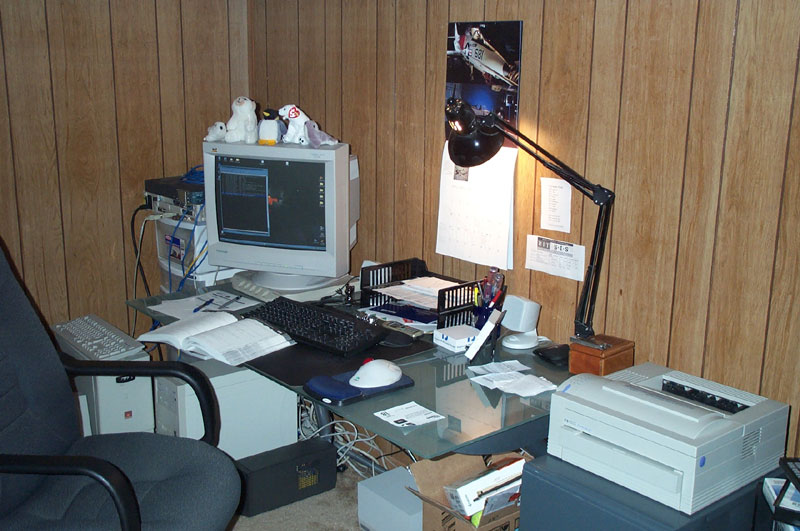
\includegraphics[width=8.33333in,height=\textheight,keepaspectratio]{images/old_desktop.jpg}

}

\caption{\label{fig-olddesk}Setup usual de um computador pessoal no
começo dos anos 2000. Fonte: \emph{Wikimedia Commons}}

\end{figure}%

\subsection{Pré-requisitos}\label{pruxe9-requisitos}

Neste capítulo introdutório não utilizaremos nenhum programa ou
linguagem. Ele foi escrito para que mesmo o aluno sem nenhum tipo de
conhecimento em computação e com o mínimo de conhecimento a respeito de
operações matemática elementares tenha capacidade de acompanhar. Basta
curiosidade!

\section{Como um computador funciona}\label{como-um-computador-funciona}

Um computador realiza duas coisas e apenas duas coisas: faz operações e
guarda de forma eficiente o resultado dessas operações. No entanto, ao
fazer essas duas coisas de forma extremamente eficiente essa máquina
chamada computador nos permite receber, armazenar, processar e
transmitir informações. Em essência, o computador nos serve ao propósito
de \textbf{resolução de problemas}. Isso significa que, através de uma
linguagem formal (especificamente operações de computação), podemos
formular problemas e programar meios de resolver de forma automatizada
tais problemas. No fim das contas, programar é o ato de criar programas,
isto é, estabelecer uma sequência de instruções em linguagem formal que
especifica como executar uma determinada operação no computador.

Mas antes de avançar na ideia de programa e algoritmos, quais são as
características de um computador como o conhecemos?

\subsection{Sistema computacional}\label{sistema-computacional}

Um sistema computacional é resultado da integração de componentes
atuando como uma entidade, com o propósito de processar dados, isto é,
realizar algum tipo de operação lógica envolvendo os dados, de modo a
produzir diferentes níveis de informações. Tais sistemas são compostos
por 3 principais elementos: hardware, software e o componente humano. O
hardware inclui os componentes físicos enquanto o software é o conjunto
de instruções que diz ao hardware o que fazer. No entanto, o software
não elabora e decide sozinho o tipo de instrução a ser enviada ao
hardware, é só através do componente humano que as instruções e
objetivos são definidos.

\begin{itemize}
\tightlist
\item
  \textbf{Hardware}: componente físico de um sistema de computação, isto
  é, todos os equipamentos utilizados pelo usuário nas ações de entrada,
  processamento, armazenamento e saída de dados. Exemplos:

  \begin{itemize}
  \tightlist
  \item
    Teclado, mouse, impressora
  \item
    Unidade central de processamento (CPU, em inglês) ou processador
  \item
    Placa mãe
  \item
    Placa de vídeo (GPU)
  \item
    Memória RAM
  \item
    Disco rígido de armazenamento
  \end{itemize}
\end{itemize}

\begin{itemize}
\tightlist
\item
  \textbf{Software}: componente lógico de um sistema de computação, isto
  é, séries de instruções que fazem o computador funcionar. São os
  famosos programas de computador, que podem ser (i) proprietários e
  utilizáveis a partir da compra de uma licença ou (ii) gratuitos.
  Exemplos:

  \begin{itemize}
  \tightlist
  \item
    Editores de texto (e.g., Microsoft Word)
  \item
    Editor de planilhas (e.g., Microsoft Excel)
  \item
    Browsers para navegação na internet (e.g., Safari e Google Chrome)
  \end{itemize}
\end{itemize}

\begin{itemize}
\tightlist
\item
  \textbf{Componente humano}: as pessoas, que utilizam o computador
  basicamente como ferramenta para atingir determinado fim, para
  resolver problemas. Sem a ação de um indivíduo o sistema computacional
  não funciona, já que (ainda) depende das instruções e direcionamento
  humano para definir o que o software deve fazer e como deve interagir
  com o hardware.
\end{itemize}

\subsection{Arquitetura de um
computador}\label{arquitetura-de-um-computador}

A arquitetura de um computador define como os componentes estão
interconectados e como eles colaboram para executar tarefas. Os
computadores, como os conhecemos hoje, são estruturados em cima da
lógica proposta inicialmente por John Von Neumann, matemático húngaro
que viveu durante a primeira metade do século XX e que contribuiu
imensamente em várias áreas das ciências. Embora tenhamos hoje uma
complexidade maior nos elementos que compõe a arquitetura de um
computador, a estrutura básica por trás dos computadores mais modernos
continua sendo aquela proposta por Von Neumann. Essa arquitetura pode
ser representado pelo diagrama abaixo:

\begin{figure}

\centering{

\includegraphics[width=7.29167in,height=\textheight,keepaspectratio]{images/arquitetura_VonNeumann.jpg}

}

\caption{\label{fig-arquitetura}Diagrama que representa o funcionamento
da arquitetura Von-Neumann}

\end{figure}%

Essencialmente, o hadware que compõe as partes da arquitetura de um
computador podem ser dividas em 3 partes:

\begin{itemize}
\item
  \textbf{Dispositivos de entrada e saída}: é através deles que o
  usuário dialoga com a máquina. Através do teclado e mouse, por
  exemplo, o usuário fornece informações ao computador a partir das
  quais processos serão realizados e seus resultados serão percebidos
  pelos dispositivos de saída (monitor e impressora, por exemplo).
\item
  \textbf{Processador ou CPU}: é o cérebro do sistema computacional, é
  nele que serão executados cálculos e instruções lógicas dos usuários.
\item
  \textbf{Memória}: aqui são armazenados temporariamente os resultados
  dos cálculos, dados e instruções. Esse armazenamento na memória,
  porém, não é feito de forma permanente, ele serve apenas como suporte
  ao processador. É como se o processador utilizasse a memória de
  caderno de anotações, retomando o resultado dos cálculos já realizados
  sempre que necessário.
\end{itemize}

\begin{tcolorbox}[enhanced jigsaw, bottomrule=.15mm, colframe=quarto-callout-important-color-frame, arc=.35mm, coltitle=black, titlerule=0mm, opacityback=0, colback=white, toptitle=1mm, breakable, bottomtitle=1mm, toprule=.15mm, left=2mm, leftrule=.75mm, title=\textcolor{quarto-callout-important-color}{\faExclamation}\hspace{0.5em}{Importante}, rightrule=.15mm, opacitybacktitle=0.6, colbacktitle=quarto-callout-important-color!10!white]

Não confunda \emph{memória} com o que chamamos de \emph{armazenamento}.
A memória do computador, normalmente na forma da chamada memória RAM
(sigla para \emph{Random Access Memory}), é responsável por armazenar
temporariamente os dados de dos programas que estão em uso, permitindo
acesso rápido pelo processador. É também chamada de memória volátil:
todo o seu conteúdo é perdido quando o computador é desligado.

Já as informações armazenadas no disco rígido (\emph{Hard Disk Drive},
HDD) ou na unidade de estado sólido (\emph{Solid-State Drive}, SSD) não
são perdidas quando o computador é desligado. Esses dispositivos mantêm
os dados armazenados de forma persistente, funcionando como a ``memória
de longo prazo'' do computador. Por isso, esse tipo de armazenamento é
chamado de memória não volátil.

Fazendo uma analogia com o funcionamento do nosso cérebro, a memória RAM
armazena informações de curto prazo, como o que você almoçou hoje. Esse
tipo de informação é importante ao longo do dia, por exemplo para saber
se você já se alimentou bem ou se ainda está longe da sua meta diária de
proteína, mas costuma ser esquecida depois que você dorme.

Já o HDD ou SSD armazena informações de longo prazo, como memórias da
infância ou experiências passadas. Essas informações não são utilizadas
constantemente no dia a dia, mas permanecem disponíveis e podem ser
úteis em conversas com amigos ou como aprendizado acumulado, por exemplo
na hora de decidir como cuidar dos seus filhos quando chegar a hora.

\end{tcolorbox}

\subsection{Bits e bytes}\label{bits-e-bytes}

Para entender como um computador armazena e processa informações, é
necessário compreender o conceito de sistema binário ou sistema de base
2\footnote{Para entender um pouco mais sobre a história do sistema
  binário acesse o
  \href{https://imasters.com.br/tecnologia/a-historia-do-codigo-binario-a-base-da-computacao-moderna}{link}.}.
Diferentemente do sistema decimal, que utilizamos no dia a dia e possui
dez dígitos (de 0 a 9), os computadores operam utilizando apenas dois
estados possíveis: 0 e 1. Pense nisso como um interruptor, em que 1
representa o estado ``ligado'' e 0 o estado ``desligado''. Os
processadores atuais de um computador são resultado da junção de bilhões
desses minúsculos ``interruptores'', também chamados de transistores.

Esses dois estados, 0 ou 1, também são chamados de bits (do inglês
\emph{binary digits}). Um bit representa a menor unidade de informação
que um computador pode armazenar. Qualquer informação processada por um
computador -- números, textos, imagens ou vídeos -- é, em última
instância, representada como uma sequência de bits.

Como trabalhar com bits individualmente seria pouco prático, eles são
agrupados em unidades maiores chamadas de bytes. Um byte é composto por
8 bits e permite representar um conjunto maior de valores. Um byte pode
representar 256 (\(2^8 = 256\)) combinações diferentes, o que é
suficiente para representar todas as letras maiúsculas e minúsculas,
números e símbolos básicos do alfabeto inglês. Não à toa, o byte se
tornou a unidade padrão de medida quando o assunto é capacidade de
armazenar informação em um computador. A Tabela Tabela~\ref{tbl-binario}
mostra como converter alguns números do sistema decimal para o sistema
binário de 8 bits, em que cada dígito dibário indica a presença ou
ausência de uma potência de 2.

\begin{longtable}[]{@{}
  >{\centering\arraybackslash}p{(\linewidth - 4\tabcolsep) * \real{0.2000}}
  >{\centering\arraybackslash}p{(\linewidth - 4\tabcolsep) * \real{0.2000}}
  >{\centering\arraybackslash}p{(\linewidth - 4\tabcolsep) * \real{0.6000}}@{}}
\caption{Representação de números decimais no sistema binário e
detalhamento do cálculo para
conversão.}\label{tbl-binario}\tabularnewline
\toprule\noalign{}
\begin{minipage}[b]{\linewidth}\centering
Número decimal
\end{minipage} & \begin{minipage}[b]{\linewidth}\centering
Número binário
\end{minipage} & \begin{minipage}[b]{\linewidth}\centering
Cálculo para conversão
\end{minipage} \\
\midrule\noalign{}
\endfirsthead
\toprule\noalign{}
\begin{minipage}[b]{\linewidth}\centering
Número decimal
\end{minipage} & \begin{minipage}[b]{\linewidth}\centering
Número binário
\end{minipage} & \begin{minipage}[b]{\linewidth}\centering
Cálculo para conversão
\end{minipage} \\
\midrule\noalign{}
\endhead
\bottomrule\noalign{}
\endlastfoot
0 & 00000000 &
\(0\cdot 2^7 + 0\cdot 2^6 + 0\cdot 2^5 + 0\cdot 2^4 + 0\cdot 2^3 + 0\cdot 2^2 + 0\cdot 2^1 + 0\cdot 2^0 = 0\) \\
1 & 00000001 &
\(0\cdot 2^7 + 0\cdot 2^6 + 0\cdot 2^5 + 0\cdot 2^4 + 0\cdot 2^3 + 0\cdot 2^2 + 0\cdot 2^1 + 1\cdot 2^0 = 1\) \\
5 & 00000101 &
\(0\cdot 2^7 + 0\cdot 2^6 + 0\cdot 2^5 + 0\cdot 2^4 + 0\cdot 2^3 + 1\cdot 2^2 + 0\cdot 2^1 + 1\cdot 2^0 = 5\) \\
48 & 00110000 &
\(0\cdot 2^7 + 0\cdot 2^6 + 1\cdot 2^5 + 1\cdot 2^4 + 0\cdot 2^3 + 0\cdot 2^2 + 0\cdot 2^1 + 0\cdot 2^0 = 48\) \\
137 & 10001001 &
\(1\cdot 2^7 + 0\cdot 2^6 + 0\cdot 2^5 + 0\cdot 2^4 + 1\cdot 2^3 + 0\cdot 2^2 + 0\cdot 2^1 + 1\cdot 2^0 = 137\) \\
255 & 11111111 &
\(1\cdot 2^7 + 1\cdot 2^6 + 1\cdot 2^5 + 1\cdot 2^4 + 1\cdot 2^3 + 1\cdot 2^2 + 1\cdot 2^1 + 1\cdot 2^0 = 255\) \\
\end{longtable}

A partir dos bytes, surgem unidades maiores, amplamente utilizadas para
medir o tamanho de arquivos, a quantidade de memória e a capacidade de
armazenamento: quilobytes, megabytes, gigabytes, terabytes e petabytes.
Essas unidades indicam, essencialmente, quantos bytes são necessários
para representar uma determinada quantidade de informação.

\begin{itemize}
\tightlist
\item
  Kilobyte (KB): \(1{,}024\) (ou \(2^{10}\)) bytes.
\item
  Megabyte (MB): \(1{,}048{,}576\) (ou \(2^{20}\)) bytes.
\item
  Gigabyte (GB): \(1{,}073{,}741{,}824\) (ou \(2^{30}\)) bytes.
\item
  Terabyte (TB): \(1{,}099{,}511{,}627{,}776\) (ou \(2^{40}\)) bytes.
\item
  Petabyte (PB): \(1{,}125{,}899{,}906{,}842{,}624\) (ou \(2^{50}\))
  bytes.
\item
  Exabyte, Zettabyte, Yottabyte\ldots{}
\end{itemize}

Compreender bits e bytes é fundamental para entender por que arquivos
têm tamanhos diferentes, por que algumas operações exigem mais memória
do que outras e por que certas tarefas computacionais são mais custosas
do ponto de vista de processamento. Esses agrupamentos de bits (bytes)
são as unidades básicas que a memória e o armazenamento usam para
guardar informação. A próxima seção explica o papel desses componentes e
como eles impactam o desempenho prático.

\subsection{Processamento, memória e armazenamento na
prática}\label{processamento-memuxf3ria-e-armazenamento-na-pruxe1tica}

Podemos entender o funcionamento de um computador como um fluxo contínuo
de \textbf{leitura}, \textbf{processamento} e \textbf{armazenamento} de
bits. Quando observamos as especificações de um computador pessoal, é
comum encontrar informações como número de núcleos do processador
(\emph{cores}), frequência do processador em gigahertz (GHz), quantidade
de memória RAM e capacidade de armazenamento em disco. Esses números
descrevem, essencialmente, a velocidade e a escala com que o computador
consegue manipular grandes volumes de informação binária em cada etapa
desse fluxo contínuo.

\textbf{Processamento} refere-se à execução de instruções sobre dados
representados em bits. O processador é o componente responsável por
realizar operações elementares que, em última instância, são operações
lógicas sobre sequências de zeros e uns. A frequência do processador
indica aproximadamente quantos ciclos de processamento podem ser
realizados por segundo. Frequências mais altas permitem que mais
instruções sejam executadas em menos tempo, embora o desempenho final
dependa também da organização do código, do tipo de tarefa e do acesso à
memória. Além disso, processadores modernos possuem múltiplos
\emph{cores} ou núcleos. O uso de múltiplos núcleos permite paralelismo,
isto é, a execução simultânea de diferentes partes de uma tarefa, de
forma análoga a dividir um trabalho entre várias pessoas para concluí-lo
mais rapidamente.

\textbf{Memória (RAM)} é o espaço onde os dados e instruções ficam
armazenados temporariamente enquanto estão sendo processados. É na
memória RAM que o computador mantém os bytes que serão acessados
repetidamente pelo processador. Quanto maior a quantidade de RAM
disponível, maior é o volume de dados que pode ser mantido ``em uso'' ao
mesmo tempo. Quando a RAM é insuficiente, o computador passa a usar o
disco como apoio, o que reduz drasticamente o desempenho.

\textbf{Armazenamento}, por sua vez, diz respeito ao local onde os dados
são guardados de forma permanente. HDDs e SSDs armazenam grandes volumes
de bytes mesmo quando o computador está desligado. A diferença principal
é que SSDs permitem acesso muito mais rápido aos dados, reduzindo o
tempo necessário para carregar programas, abrir arquivos e transferir
grandes conjuntos de dados para a memória.

Vistos em conjunto, processamento, memória e armazenamento formam um
sistema integrado: dados são lidos do disco, carregados na memória,
processados pela CPU e, quando necessário, gravados novamente no
armazenamento. Para tarefas simples, esse fluxo passa despercebido. Para
programação, análise de dados e computação numérica compreender essas
etapas ajuda a interpretar erros, gargalos de desempenho e limitações
práticas do ambiente computacional.

\begin{tcolorbox}[enhanced jigsaw, bottomrule=.15mm, colframe=quarto-callout-tip-color-frame, arc=.35mm, coltitle=black, titlerule=0mm, opacityback=0, colback=white, toptitle=1mm, breakable, bottomtitle=1mm, toprule=.15mm, left=2mm, leftrule=.75mm, title=\textcolor{quarto-callout-tip-color}{\faLightbulb}\hspace{0.5em}{O que significam as especificações do seu computador?}, rightrule=.15mm, opacitybacktitle=0.6, colbacktitle=quarto-callout-tip-color!10!white]

Considere um computador com processador com 16 núcleos e frequência de
3.2 GHz, 32 GB de memória RAM e 1 TB de SSD. Esses números descrevem
como ele lida com bits e bytes em diferentes etapas do processamento.

\begin{itemize}
\item
  \textbf{16 núcleos (cores)} indicam que o processador pode executar
  várias tarefas ao mesmo tempo. Em aplicações que permitem paralelismo
  -- como certas operações numéricas ou análises sobre grandes conjuntos
  de dados -- isso é semelhante a dividir o trabalho entre dezesseis
  pessoas em vez de apenas uma.
\item
  \textbf{3.2 GHz} refere-se à velocidade com que cada núcleo executa
  instruções elementares. Em termos simples, indica quantos passos o
  processador consegue dar por segundo ao manipular dados representados
  em sistema binário.
\item
  \textbf{32 GB de RAM} significam que até esse volume de dados pode
  permanecer disponível para acesso rápido enquanto programas estão em
  execução. Bases de dados grandes, matrizes extensas e múltiplos
  processos consomem memória rapidamente.
\item
  \textbf{1 TB de SSD} indica a capacidade de armazenamento permanente.
\end{itemize}

Em análise de dados e programação, problemas de desempenho raramente
estão ligados apenas à velocidade do processador. Com frequência, eles
surgem porque os dados são grandes demais para caber na memória ou
porque operações são realizadas de forma pouco eficiente. Entender essas
especificações ajuda a interpretar erros, lentidão e limitações práticas
do ambiente computacional.

\end{tcolorbox}

\section{Arquivos e diretórios}\label{arquivos-e-diretuxf3rios}

Mais do que armazenar informação, é importante entender \emph{onde} e
\emph{como} a informação é armazenada. Assim como na vida cotidiana, é
preciso ter organização no armazenamento para saber como e onde procurar
determinada informação no computador. Se você é uma pessoa organizada,
você sabe que o iogurte estará sempre guardada na geladeira e em algum
pote fechado, não é preciso procurar debaixo do chuveiro em um saco de
pão.

\subsection{Estrutura hierárquica}\label{estrutura-hieruxe1rquica}

Os diretórios servem justamente para organizar o armazenamento do
computador. É como se você pudesse separar o seu SSD primeiro em
cômodos, depois em armários dentro de cada cômodo, em gavetas dentro de
cada armário e assim por diante. Formalmente, um diretório pode ser
entendido como um contêiner no qual arquivos e outros diretórios podem
estar organizados, formando uma estrutura hierárquica. Essa organização
permite localizar, acessar e manipular arquivos de forma sistemática,
especialmente em projetos maiores.

Por exemplo, a organização de um projeto de análise de dados pode ter a
seguinte forma:

\begin{Shaded}
\begin{Highlighting}[]
\NormalTok{C:\textbackslash{}}
\NormalTok{└── projeto\textbackslash{}}
\NormalTok{    ├── data\textbackslash{}}
\NormalTok{    │   └── dados.csv}
\NormalTok{    ├── scripts\textbackslash{}}
\NormalTok{    │   └── analise.py}
\NormalTok{    └── resultados\textbackslash{}}
\NormalTok{        └── figura1.png}
\end{Highlighting}
\end{Shaded}

Nesse exemplo, \texttt{projeto} é um diretório que está dentro da
partição C e que contém outros diretórios. O arquivo \texttt{dados.csv},
por exemplo, está dentro do diretório \texttt{data}, que é um diretório
localizado dentro do diretório \texttt{projeto}. Para acessar esse
arquivo \texttt{dados.csv} dentro dessa estrutura hierárquica de
diretórios utilizamos duas formas principais: o caminho absoluto ou o
caminho relativo.

\begin{itemize}
\tightlist
\item
  \textbf{Caminho absoluto}: descreve a localização completa a partir da
  raiz do sistema de arquivos. Nesse caso, o caminho absoluto seria
  \texttt{C:\textbackslash{}projeto\textbackslash{}data\textbackslash{}dados.csv}.
\item
  \textbf{Caminho relativo}: descreve a localização em relação ao
  diretório atual. Isso quer dizer que, se estivermos trabalhando em um
  programa a partir do diretório \texttt{projeto}, para acessar o
  arquivo de dados basta descrever o caminho relativo a partir dali:
  \texttt{data/dados.csv}.
\end{itemize}

\subsection{Extensões de arquivos}\label{extensuxf5es-de-arquivos}

Para além do \emph{onde}, a informação em si pode ser armazenada de
várias formas. Você pode guardar o iogurte em uma jarra de vidro ou
mantê-lo no recipiente original. Um conjunto de informação é armazenada
em um arquivo que pode ter vários formatos ou \textbf{extensões}. A
extensão do arquivo corresponde ao sufixo após o ponto no nome do
arquivo e indica como os dados estão organizados internamente e quais
programas sabem interpretá-los corretamente. Do ponto de vista
conceitual, a extensão não ``muda'' o dado em si, mas define a estrutura
lógica usada para representar a informação. O mesmo conjunto de
informações pode ser salvo em formatos diferentes, dependendo do
objetivo (leitura humana, processamento automático, troca entre sistemas
etc.).

Um formato muito comum em análise de dados é o CSV (\texttt{.csv},
\emph{Comma-Separated Values}). Trata-se de um arquivo de texto em que
os dados são organizados em linhas e colunas, sendo as colunas separadas
por um delimitador, geralmente uma vírgula. Cada linha representa uma
observação e a primeira linha costuma conter os nomes das variáveis.
Arquivos CSV são amplamente utilizados porque (i) são simples e
legíveis; (ii) podem ser abertos em editores de texto, planilhas e
softwares estatísticos; e (iii) são facilmente importados por linguagens
como Python.

Outro formato bastante utilizado é o JSON (\texttt{.json},
\emph{JavaScript Object Notation}). Embora também seja um arquivo de
texto, sua estrutura é diferente. Em vez de linhas e colunas, os dados
são organizados como pares chave--valor, de forma semelhante a um
dicionário, podendo conter listas e estruturas aninhadas. Esse formato é
muito usado para troca de dados entre sistemas e aplicações, além do uso
para armazenamento de configurações.

Outras extensões comuns incluem:

\begin{itemize}
\tightlist
\item
  \texttt{.txt}: texto simples, sem estrutura fixa.
\item
  \texttt{.xlsx}: arquivos de planilha do Microsoft Excel.
\item
  \texttt{.py}: arquivos de código Python.
\end{itemize}

É importante enfatizar que a extensão não garante o conteúdo do arquivo:
um \texttt{.csv} mal formatado pode não ser lido corretamente, e um
arquivo \texttt{.txt} pode conter dados altamente estruturados. Ainda
assim, seguir convenções de extensão é essencial para organização de
projetos, reprodutibilidade e interoperabilidade entre ferramentas.
Considere a tabela de notas abaixo:

\begin{longtable}[]{@{}ccccc@{}}
\toprule\noalign{}
nome & nusp & ingresso & materia & media \\
\midrule\noalign{}
\endhead
\bottomrule\noalign{}
\endlastfoot
Joao & 12345678 & 2026 & EAE1106 & 8 \\
Miguel & 5253678 & 2023 & EAE1106 & 4 \\
Alice & 9743678 & 2025 & EAE1106 & 9 \\
\end{longtable}

O armazenamento desses dados em formato CSV e JSON é feito da seguinte
maneira:

\begin{itemize}
\item
  Formato CSV

\begin{Shaded}
\begin{Highlighting}[]
\NormalTok{nome,nusp,ingresso,materia,media}
\NormalTok{Joao,12345678,2026,EAE1106,8}
\NormalTok{Miguel,52543678,2023,EAE1106,4}
\NormalTok{Alice,9743678,2025,EAE1106,9}
\end{Highlighting}
\end{Shaded}
\item
  Formato JSON

\begin{Shaded}
\begin{Highlighting}[]
\NormalTok{[}
\NormalTok{\{}
\NormalTok{   "nome": "Joao",}
\NormalTok{   "nusp": 12345678,}
\NormalTok{   "ingresso": 2026,}
\NormalTok{   "materia": "EAE1106",}
\NormalTok{   "media": 8}
\NormalTok{\},}
\NormalTok{\{}
\NormalTok{   "nome": "Miguel",}
\NormalTok{   "nusp": 52543678,}
\NormalTok{   "ingresso": 2023,}
\NormalTok{   "materia": "EAE1106",}
\NormalTok{   "media": 4}
\NormalTok{\},}
\NormalTok{\{}
\NormalTok{   "nome": "Alice",}
\NormalTok{   "nusp": 9743678,}
\NormalTok{   "ingresso": 2025,}
\NormalTok{   "materia": "EAE1106",}
\NormalTok{   "media": "9"}
\NormalTok{\}}
\NormalTok{]}
\end{Highlighting}
\end{Shaded}
\end{itemize}

Mas qual a importância disso tudo? Entender como os computadores
armazenam números e como arquivos e diretórios são organizados e
acessados pelo sistema operacional ajuda a compreender limitações e
comportamentos observados na prática. Por exemplo, explica por que um
sistema de 32 bits é capaz de alocar apenas até 4 GB de memória RAM ou
por que arquivos com milhões de linhas podem ser difíceis de abrir ou
processar em um computador local.

Ter um conhecimento mínimo sobre o funcionamento do computador e sobre
como os programas interagem com sua arquitetura permite entender o que
ocorre ``por trás das cortinas''. Com isso, podemos usar o computador
como uma ferramenta para resolver problemas --- e não como um fim em si.
Para chegar a esse ponto, precisamos de meios formais para nos comunicar
com o sistema operacional e, posteriormente, expressar instruções de
forma lógica e precisa.

\section{Terminal}\label{terminal}

Um passo intermediário entre o funcionamento interno do computador e as
linguagens de programação é o terminal. O terminal é uma interface
textual que permite interagir diretamente com o sistema operacional por
meio de comandos simples. Em vez de clicar em ícones ou navegar por
menus gráficos, o usuário descreve explicitamente o que deseja que o
computador faça.

O uso do terminal torna visíveis conceitos introduzidos na seção
anterior, como arquivos e diretórios, além de fornecer um primeiro
contato com a lógica de comandos que será essencial ao longo do curso. A
Figura Figura~\ref{fig-terminal} ilustra o ambiente típico do terminal
nos dois principais sistemas operacionais em uso atualmente.

\begin{figure}

\begin{minipage}{0.50\linewidth}

\pandocbounded{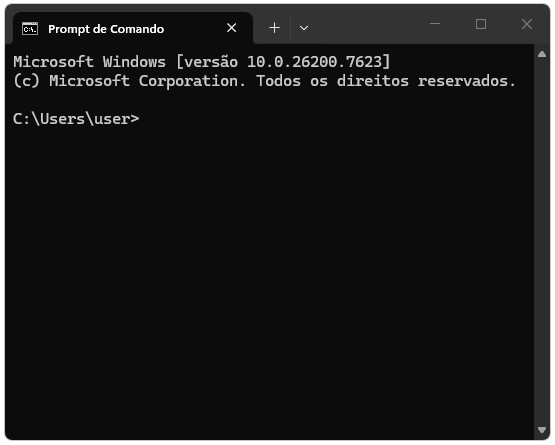
\includegraphics[keepaspectratio]{images/terminal_windows.jpg}}

\subcaption{\label{}Windows}
\end{minipage}%
%
\begin{minipage}{0.50\linewidth}

\pandocbounded{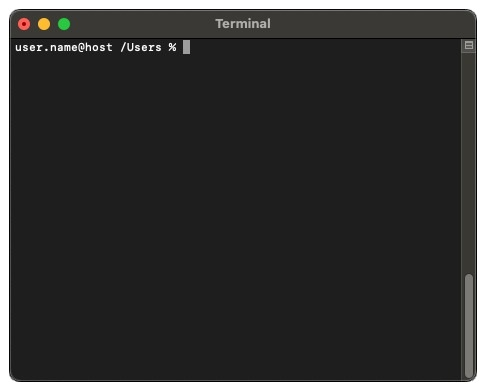
\includegraphics[keepaspectratio]{images/terminal_macos.jpeg}}

\subcaption{\label{}MacOS}
\end{minipage}%

\caption{\label{fig-terminal}Interface usual do terminal}

\end{figure}%

Comandos básicos no terminal (ou prompt de comando) do Windows incluem:

\begin{itemize}
\tightlist
\item
  \texttt{dir}: lista arquivos e diretórios no ambiente atual
\item
  \texttt{cd}: muda de diretório
\item
  \texttt{mkdir}: cria um novo diretório
\end{itemize}

No exemplo do painel A da Figura Figura~\ref{fig-terminal},
\texttt{cd\ "C:\textbackslash{}projeto"} muda o ambiente atual do
diretório \texttt{C:\textbackslash{}Users\textbackslash{}user} para
\texttt{C:\textbackslash{}projeto}. Note, porém, que se a pasta
\texttt{projeto} estiver em outra partição do seu armazenamento, é
preciso primeiro mudar para essa partição para depois utilizar o comando
\texttt{cd}. A Figura Figura~\ref{fig-cmd} ilustra esses dois casos.

\begin{figure}

\begin{minipage}{0.50\linewidth}

\pandocbounded{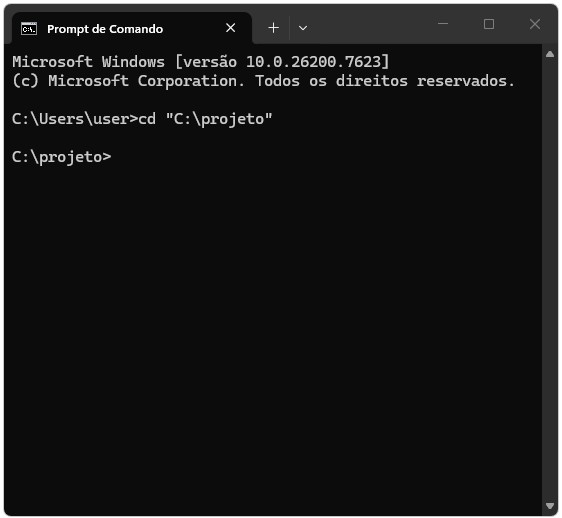
\includegraphics[keepaspectratio]{images/cmd1.jpg}}

\subcaption{\label{}Diretório na mesma partição}
\end{minipage}%
%
\begin{minipage}{0.50\linewidth}

\pandocbounded{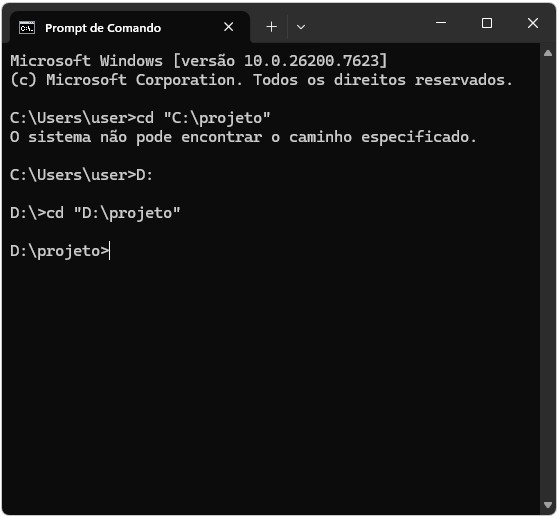
\includegraphics[keepaspectratio]{images/cmd2.jpg}}

\subcaption{\label{}Diretório em outra partição}
\end{minipage}%

\caption{\label{fig-cmd}Exemplo de uso do terminal para mudar o ambiente
atual}

\end{figure}%

Mesmo que você utilize interfaces gráficas, compreender o terminal
facilita o entendimento de como o computador está organizado e de como o
sistema operacional executa tarefas básicas. Ao longo do curso, o
terminal será utilizado principalmente para executar programas, navegar
entre diretórios e instalar novos pacotes e ferramentas.

Apesar de útil, o terminal ainda exige que as instruções sejam dadas
comando a comando, de forma relativamente limitada e pouco reutilizável.
Se queremos resolver problemas mais gerais e automatizar tarefas de
forma sistemática, é necessário um nível adicional de abstração.

\section{Linguagens de
programação}\label{linguagens-de-programauxe7uxe3o}

Para atingir esse nível adicional de abstração, precisamos de um meio de
comunicar instruções ao computador de maneira precisa e sem
ambiguidades. Esse meio são as linguagens de programação, que definem
regras formais para descrever operações, decisões e cálculos que o
computador pode executar. Diferentemente das linguagens naturais, como o
português que eu e você falamos, as linguagens de programação são
linguagens formais, que foram criadas pelas pessoas para aplicações
específicas. A notação usada pelos matemáticos é uma linguagem formal
adequada para representar relações entre números e símbolos; químicos
utilizam linguagens formais para representar a estrutura de moléculas.
Utilizamos as linguagens de programação para nos comunicar de forma
inequívoca com os computadores.

\subsection{Sintaxe e semântica}\label{sintaxe-e-semuxe2ntica}

Toda linguagem de programação possui dois níveis fundamentais: sintaxe e
semântica.

A \textbf{sintaxe} refere-se às regras de escrita da linguagem. Ela
define quais símbolos e quais sequências de símbolos são válidas: onde
usar parênteses, palavras-chave, operadores e a ordem correta dos
elementos. Erros de sintaxe são, em geral, fáceis de identificar porque
a execução do programa é interrompida e uma mensagem de erro é
apresentada. Exemplos comuns incluem esquecer um caractere obrigatório
em determinada sequência, utilizar parênteses, colchetes ou aspas sem o
fechamento correspondente ou escrever palavras-chave de forma incorreta.
Nesses casos, o computador não consegue sequer interpretar a estrutura
do código, independentemente da intenção do programador.

Por outro lado, a \textbf{semântica} refere-se ao significado das
instruções. Um código pode estar sintaticamente correto, mas produzir
resultados errados por não representar corretamente a intenção do
programador. Erros semânticos são mais sutis, pois o código respeita
todas as regras formais da linguagem e é executado normalmente, mas o
resultado obtido está incorreto. Por exemplo, um programa pode calcular
uma média dividindo a soma dos valores pelo número errado de observações
ou usar uma variável diferente da pretendida em uma expressão. Esses
erros não geram mensagens automáticas do computador e só podem ser
detectados pela análise crítica dos resultados produzidos.

Essa distinção é central em programação. O computador consegue verificar
automaticamente erros de sintaxe, mas não é capaz de julgar se o
significado do programa está correto do ponto de vista do problema que
se deseja resolver.

\subsection{Diferenças entre linguagens naturais e
formais}\label{diferenuxe7as-entre-linguagens-naturais-e-formais}

Embora as linguagens formais e naturais tenham muitas características em
comum -- símbolos, estrutura, sintaxe e semântica -- há algumas
diferenças:

\begin{enumerate}
\def\labelenumi{\arabic{enumi}.}
\item
  \textbf{Ambiguidade}: as linguagens naturais são cheias de ambiguidade
  e as pessoas lidam com isso usando pistas contextuais e outras
  informações. As linguagens formais são criadas para ser quase ou
  completamente inequívocas, ou seja, qualquer afirmação tem exatamente
  um significado, independentemente do contexto
\item
  \textbf{Redundância}: para compensar a ambiguidade e reduzir
  equívocos, as linguagens naturais usam muita redundância. Por causa
  disso, muitas vezes são verborrágicas. As linguagens formais são menos
  redundantes e mais concisas.
\item
  \textbf{Literalidade}: as linguagens naturais são cheias de expressões
  e metáforas. Se eu digo ``caiu a ficha'', provavelmente não há ficha
  nenhuma na história, nem nada que tenha caído (esta é uma expressão
  para dizer que alguém entendeu algo depois de certo período de
  confusão). As linguagens formais têm significados exatamente iguais ao
  que expressam.
\end{enumerate}

Como todos nós crescemos falando linguagens naturais, às vezes é difícil
se ajustar a linguagens formais. As linguagens formais são mais densas
que as naturais, então exigem mais tempo para a leitura. Além disso, a
estrutura é importante, então nem sempre é melhor ler de cima para baixo
e da esquerda para a direita. Em vez disso, aprenda a analisar o
programa primeiro, identificando os símbolos e interpretando a
estrutura. E os detalhes fazem diferença. Pequenos erros em ortografia e
pontuação, que podem não importar tanto nas linguagens naturais, podem
fazer uma grande diferença em uma língua formal.

\subsection{Alto nível X baixo
nível}\label{alto-nuxedvel-x-baixo-nuxedvel}

As linguagens de programação também diferem quanto ao seu nível de
abstração. Na ciência da computação, \textbf{linguagens de programação
de alto nível} abstraem detalhes do funcionamento interno do computador,
permitindo que o programador se concentre na lógica do problema. São
linguagens mais próximas das linguagens humanas e mais distantes das
linguagens de máquina (e do sistema binário). Tais linguagens podem usar
elementos de linguagem natural, serem mais fáceis de usar, ou podem
ocultar totalmente áreas significativas de sistemas de computação, como
o gerenciamento de memória. Isso torna o processo de desenvolvimento de
um programa mais simples e eficiente. Python, R e Java são alguns
exemplos de linguagens de alto nível.

Por outro lado, uma \textbf{linguagem de baixo nível} é uma linguagem de
programação que fornece pouca ou nenhuma abstração de conceitos de
programação e está muito próxima de escrever instruções de máquina
reais. A palavra ``baixo'' refere-se à pequena ou inexistente quantidade
de abstração entre a linguagem e a linguagem de máquina; por causa
disso, as linguagens de baixo nível são às vezes descritas como
\emph{próximas do hardware}. Programas escritos em linguagens de baixo
nível tendem a ser relativamente não portáteis e dependentes do
computador para o qual foram escritas. Assembly é uma das linguagens de
mais baixo nível à disposição do programador.

Em cursos como Economia e outras ciências aplicadas, linguagens de alto
nível são preferidas porque reduzem o custo cognitivo, o tempo
necessário para produzir código e aumentam a produtividade.

\subsection{Linguagem Compilada X
Interpretada}\label{linguagem-compilada-x-interpretada}

Outra distinção importante diz respeito à forma como o código é
executado. Em \textbf{linguagens compiladas} o código é traduzido
integralmente para código de máquina antes da execução. Elas também dão
ao desenvolvedor mais controle sobre os aspectos de hardware, como
gerenciamento de memória e uso da CPU. As linguagens compiladas precisam
de uma etapa de ``construção'' -- elas precisam ser compiladas
manualmente primeiro. Somente após essa etapa que o código pode rodar
por completo. Linguagens como C e C++ seguem esse modelo.

Em \textbf{linguagens interpretadas}, as instruções não são executadas
diretamente pela máquina de destino, mas lidas e executadas, linha por
linha, por algum outro programa, um intérprete. Isso permite maior
flexibilidade e facilita a experimentação, embora geralmente com menor
desempenho em tempo de máquina. Python e R são exemplos clássicos de
linguagens interpretadas.

Embora usualmente mais lentas, essa simplicidade e flexibilidade em
escrever código torna linguagens interpretadas particularmente adequadas
para aprendizado, análise de dados e trabalho empírico. Lembre-se, no
fim das contas, o tempo relevante não é apenas o tempo de máquina, mas o
tempo que você leva para escrever e depurar código.

\subsection{Paradigmas}\label{paradigmas}

Linguagens de programação também podem ser classificadas segundo o
paradigma que adotam, isto é, o estilo predominante de organização do
código. Entre os principais paradigmas de programação podemos citar
programação imperativa, procedural, funcional, declarativa e programação
orientada a objetos. Na programação imperativa, por exemplo, o
programador diz como, o quê e em qual ordem exatamente um programa ou
rotina deve realizar. É neste paradigma que surgiram as famosas
estruturas condicionais e atribuição de valor à variáveis. Por outro
lado, na programação orientada a objetos o programa é estruturado em
objetos que combinam dados e comportamento. Mais detalhes sobre
paradigmas de programação podem ser obtidos
\href{https://www.freecodecamp.org/news/an-introduction-to-programming-paradigms/\#what-is-a-programming-paradigm}{aqui}.

Muitas linguagens modernas, incluindo Python, são multiparadigma,
permitindo combinar diferentes estilos conforme o problema.

\subsection{Tipagem}\label{tipagem}

Por fim, as linguagens diferem quanto à forma como tratam os tipos de
dados. Em linguagens de tipagem estática, o tipo de cada variável é
definido explicitamente no código e verificado antes da execução. O
Python utiliza tipagem dinâmica, isso significa que o próprio
interpretador do Python infere o tipo dos dados que uma variável recebe,
sem a necessidade que o usuário diga de que tipo determinada variável é.
Além disso, o Python é uma linguagem fortemente tipada, o que significa
que o interpretador do Python avalia as expressões por conta própria e
não faz conversões automáticas de valores entre tipos de dados não
compatíveis. Ao fazer operações com tipos incompatíveis, o Python não
converte automaticamente esses tipos pra você, ele vai dar erro.

Tipagem dinâmica reduz a quantidade de código inicial e facilita
experimentação, mas exige atenção adicional para evitar erros lógicos já
que o usuário não define explicitamente o tipo do dado. No entanto, a
tipagem forte reduz a chance de resultados inesperados por conta de
tipos definidos ou convertidos de forma equivocada já que a linguagem
não tenta corrigir o erro por conta própria.

\section{Conclusão}\label{conclusuxe3o}

Neste capítulo, foram apresentados os fundamentos básicos sobre o
funcionamento de um sistema computacional, incluindo arquitetura,
memória, organização de arquivos, interação com o sistema operacional e
o papel das linguagens de programação. Esses conceitos fornecem a base
necessária para compreender como o computador executa instruções e por
que certas limitações surgem na prática.

A partir daqui, o curso passa a utilizar Python como linguagem de
trabalho. Python é uma linguagem de alto nível, interpretada e
multiparadigma que é amplamente empregada em análise de dados e pesquisa
empírica em Economia, pois permite expressar soluções de forma clara e
concisa, além de oferecer um amplo conjunto de bibliotecas científicas.
No próximo capítulo, iniciaremos o trabalho prático: escrever código em
Python, executar programas, interpretar erros e manipular dados
diretamente no computador.

\section{Exercícios}\label{exercuxedcios}

\begin{enumerate}
\def\labelenumi{\arabic{enumi}.}
\item
  Um arquivo de dados possui 10 milhões de linhas e 80 colunas, com
  todas as células contendo valores numéricos. Suponha que cada valor
  numérico ocupe 8 bytes na memória.

  \begin{enumerate}
  \def\labelenumii{\alph{enumii}.}
  \tightlist
  \item
    Faça uma estimativa aproximada da quantidade de memória RAM (em GB)
    necessária para carregar esse arquivo inteiro na memória.
  \item
    Explique por que um computador com pouca memória RAM pode ter
    dificuldade para trabalhar com esse arquivo, mesmo que o arquivo
    ``caiba'' no disco rígido.
  \end{enumerate}
\item
  Sobre o sistema binário responda:

  \begin{enumerate}
  \def\labelenumii{\alph{enumii}.}
  \tightlist
  \item
    Converta o número decimal 13 para a representação binária.
  \item
    Converta o número binário 101101 para decimal.
  \item
    Argumente, em poucas linhas, sobre a vantagem de computadores
    utilizarem o sistema binário em vez do sistema decimal.
  \end{enumerate}
\item
  Considere a seguinte estrutura de diretórios:

\begin{Shaded}
\begin{Highlighting}[]
\NormalTok{D:/home/usuario/projeto/}
\NormalTok{├── dados/}
\NormalTok{│   └── alunos.csv}
\NormalTok{│   └── professores.csv}
\NormalTok{│   └── materias.csv}
\NormalTok{├── scripts/}
\NormalTok{│   └── analise.py}
\NormalTok{│   └── amostra\_final.py}
\NormalTok{└── resultados/}
\NormalTok{   └── figura.png}
\NormalTok{   └── tabela.csv}
\end{Highlighting}
\end{Shaded}

  \begin{enumerate}
  \def\labelenumii{\alph{enumii}.}
  \tightlist
  \item
    Escreva o caminho absoluto para o acessar o arquivo
    \texttt{materias.csv}.
  \item
    Suponha que você esteja no diretório scripts. Escreva o caminho
    relativo para acessar \texttt{materias.csv}. Dica: a pasta dados e
    scripts estão no mesmo nível hierárquico.
  \end{enumerate}
\item
  Considere a matemática como uma linguagem formal, com regras bem
  definidas de escrita (sintaxe) e de significado (semântica). Suponha
  que o objetivo seja calcular as raízes de uma equação do segundo grau
  da forma \(ax^2 + bx + c = 0\). Para tal você utilizará a fórmula de
  Bháskara.

  \begin{enumerate}
  \def\labelenumii{\alph{enumii}.}
  \item
    Suponha que você opte por programar essa fórmula tal qual
    apresentada abaixo em uma determinada linguagem de programação. Qual
    seria a saída esperada? Discuta o resultado.

    \[x = \frac{-b \ge \sqrt{b^2 - 4ac}}{2a}\]
  \item
    Suponha que você opte por programar essa fórmula tal qual
    apresentada abaixo em uma determinada linguagem de programação. Qual
    seria a saída esperada? Discuta o resultado.

    \[x = \frac{-b \pm \sqrt{b^2 - 4ac}}{2}\]
  \end{enumerate}
\end{enumerate}

\chapter{Primeiros passos no Python}\label{sec-primeiros_passos}

\section{Introdução}\label{introduuxe7uxe3o-1}

Criado em 1989 por Guido van Rossum no Centro de Matemática e Tecnológia
da Informação na Holanda, o Python é uma linguagem de programação
amplamente utilizada em ciência de dados, estatística e desenvolvimento
científico em geral. Ao longo desta disciplina, Python será utilizado
como ferramenta central para manipular dados, realizar cálculos
numéricos, produzir gráficos e implementar rotinas que aparecem com
frequência em trabalhos empíricos em economia.

Neste momento inicial do curso, o objetivo não é compreender toda a
linguagem nem escrever programas complexos. O foco desta aula é muito
mais operacional: aprender a executar comandos simples, entender como o
ambiente de programação funciona e desenvolver familiaridade com a
lógica básica de interação com o computador por meio de código. É
importante destacar que programar não é memorizar comandos, mas aprender
a ler, testar e corrigir código. Erros farão parte do processo desde o
início. Isso não indica falta de habilidade nem desconhecimento do
conteúdo; pelo contrário, erros são a principal fonte de informação
sobre como o programa está sendo interpretado pelo computador.

\begin{figure}

\centering{


\includegraphics[width=8.33333in,height=\textheight,keepaspectratio]{images/clayton_coding.png}

}

\caption{\label{fig-clayton}Meu cachorro Clayton dando seus primeiros
passos em Python.}

\end{figure}%

Ao final deste capítulo, espera-se que você seja capaz de:

\begin{itemize}
\tightlist
\item
  Executar comandos simples em Python.
\item
  Reconhecer mensagens de erro e localizar a origem do problema.
\item
  Desenvolver uma postura ativa de experimentação e verificação.
\end{itemize}

Essas competências serão usadas continuamente ao longo do curso e são
essenciais para o desenvolvimento em tópicos futuros, como construção de
funções, manipulação de objetos, análise de dados e visualização. Antes
de aprender novos comandos, no entanto, é fundamental compreender o
ambiente no qual o programa roda e como ocorre a interação entre o
usuário e o interpretador.

\subsection{Pré-requisitos}\label{pruxe9-requisitos-1}

Este foi escrito para que o aluno que acompanhou e absorveu o conteúdo
do capítulo anterior, sobre fundamentos de computação, seja plenamente
capaz de acompanhar. Não há outros pré-requisitos.

\section{O Python}\label{o-python}

Assim como tudo na vida, o Python é uma linguagem de programação com
muitas qualidades mas que também possui seus defeitos (em geral ligados
à velocidade de execução dos programas). Em sendo uma linguagem de alto
nível, é uma linguagem bastante indicada, por exemplo, para aplicações
que demandam replicabilidade, dada a facilidade de escrever e
interpretar o código. Por outro lado, aplicações que demandam uma
interação mais eficiente entre o código e o gerenciamento de memória da
máquina, por exemplo, podem se beneficiar de outras linguagens.

No entanto, o conjunto de qualidades do Python e as inúmeras bibliotecas
que foram desenvolvidas nos últimos anos parecem ter mais do que
compensado as falhas da linguagem. Hoje o Python é uma das principais
linguagens de programação (senão a principal) quando o assunto é ciência
dos dados e aprendizado de máquina (\emph{data science} e \emph{machine
learning}, respectivamente). É também uma das principais linguagens de
programação por trás de vários dos sistemas de grandes empresas, como
Uber, GoldmanSachs, Netflix e Google (fonte:
\href{https://brainstation.io/career-guides/who-uses-python-today}{link}).

Por todos esses fatores, Python é uma das linguagens com a comunidade
mais ativa em fóruns online voltados à programação e é a
\textbf{linguagem que mais cresce no mundo}. As figuras abaixo ilustram
bem esse crescimento da linguagem nos últimos anos:

\begin{figure}

\centering{

\includegraphics[width=7.29167in,height=\textheight,keepaspectratio]{images/pypl_index.jpg}

}

\caption{\label{fig-pypl}Indíce PyPL de popularidade de linguagens.
Janeiro de 2026}

\end{figure}%

\subsection{Como instalar}\label{como-instalar}

Existe mais de uma forma de instalar o Python no seu sistema e ainda
mais formas de interagir com a linguagem. Você pode baixar o Python
\emph{puro} (https://www.python.org/downloads/) e instalá-lo diretamente
em sua máquina, porém, essa distribuição vem com poucos pacotes já
instalados e instalá-los um a um requer paciência. Além disso, a
instalação do Python puro pode demandar algumas alterações em
configurações do sistema via prompt de comando do Windows, por exemplo,
para que seja possível dialogar com a linguagem.

Uma forma mais simples de instalar o Python em seu computador é através
da distribuição Anaconda. Além de ser gratuita e já conter vários dos
pacotes que iremos utilizar, ela nos fornece diversas ferramentas que
facilitam nossa interação com a linguagem. É hoje uma das distribuições
do Python mais populares no mundo! \textbf{Recomendo fortemente utilizar
esse caminho}.

\emph{O passo a passo a seguir foi feito para o sistema Windows 10.
Embora o caminho seja parecido, podem haver algumas divergências em
relação ao passo a passo para sistemas Linux e MacOS.}

\begin{enumerate}
\def\labelenumi{\arabic{enumi}.}
\tightlist
\item
  Baixar e instalar o Anaconda é fácil. Basta acessar a aba de downloads
  no site do \href{https://www.anaconda.com/download}{Anaconda},
  fornecer um email para cadastro e baixar o arquivo executável
  necessário para a instalação a depender do seu sistema operacional.
\end{enumerate}

\begin{figure}

\centering{

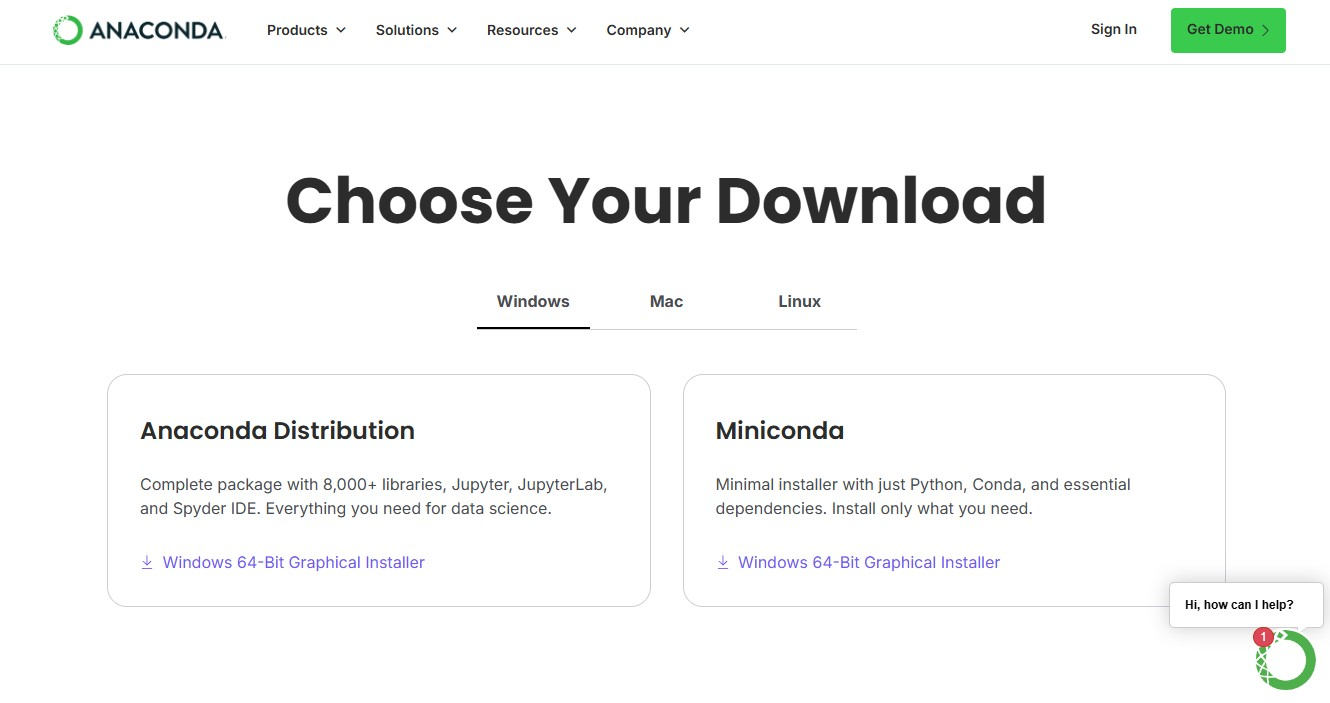
\includegraphics[width=8.33333in,height=\textheight,keepaspectratio]{images/anaconda_download.jpg}

}

\caption{\label{fig-anaconda1}Tela de download da distribuição Anaconda.
Janeiro de 2026}

\end{figure}%

\begin{enumerate}
\def\labelenumi{\arabic{enumi}.}
\setcounter{enumi}{1}
\tightlist
\item
  Depois de baixado, basta clicar duas vezes sobre o arquivo e ir
  acompanhando o instalador, mantendo sempre as opções padrão e
  escolhendo a opção de instalação preferida. Note, porém que a
  instalação para todos os usuários do computador requer permissões de
  administrador.
\end{enumerate}

\begin{figure}

\centering{

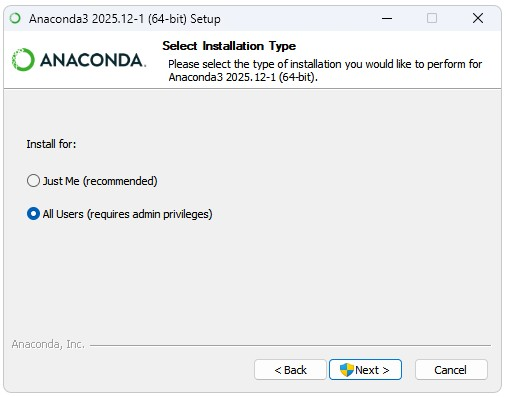
\includegraphics[width=4.16667in,height=\textheight,keepaspectratio]{images/anaconda_install.jpg}

}

\caption{\label{fig-anaconda2}Tela de instalação da distribuição
Anaconda. Janeiro de 2026}

\end{figure}%

\begin{enumerate}
\def\labelenumi{\arabic{enumi}.}
\setcounter{enumi}{2}
\tightlist
\item
  Pronto, o Anaconda está instalado e os principais pacotes e programas
  que utilizaremos também!
\end{enumerate}

\subsection{Anaconda e suas
particularidades}\label{anaconda-e-suas-particularidades}

Como dito acima, Anaconda é uma distribuição do Python para computação
científica (e.g, ciência de dados e aprendizado de máquina), que visa
simplificar o gerenciamento e a implantação de pacotes. As versões de
pacotes no Anaconda são gerenciadas pelo sistema de gerenciamento de
pacotes \emph{conda}. Através do \emph{conda} é possível criar ambientes
e instalar pacotes distintos de forma a evitar incompatibilidades entre
versões de pacotes já instalados.

Além disso, o Anaconda traz consigo o Anaconda Navigator, um ambiente
\emph{user-friendly} para a gestão de pacotes e aplicativos necessários
para a utilização do Python sem que seja preciso ter qualquer
conhecimento acerca da utilização correta de terminais. Ao abrir o
Anaconda Navigator no Windows, você deve ver algo assim:

\begin{figure}

\centering{

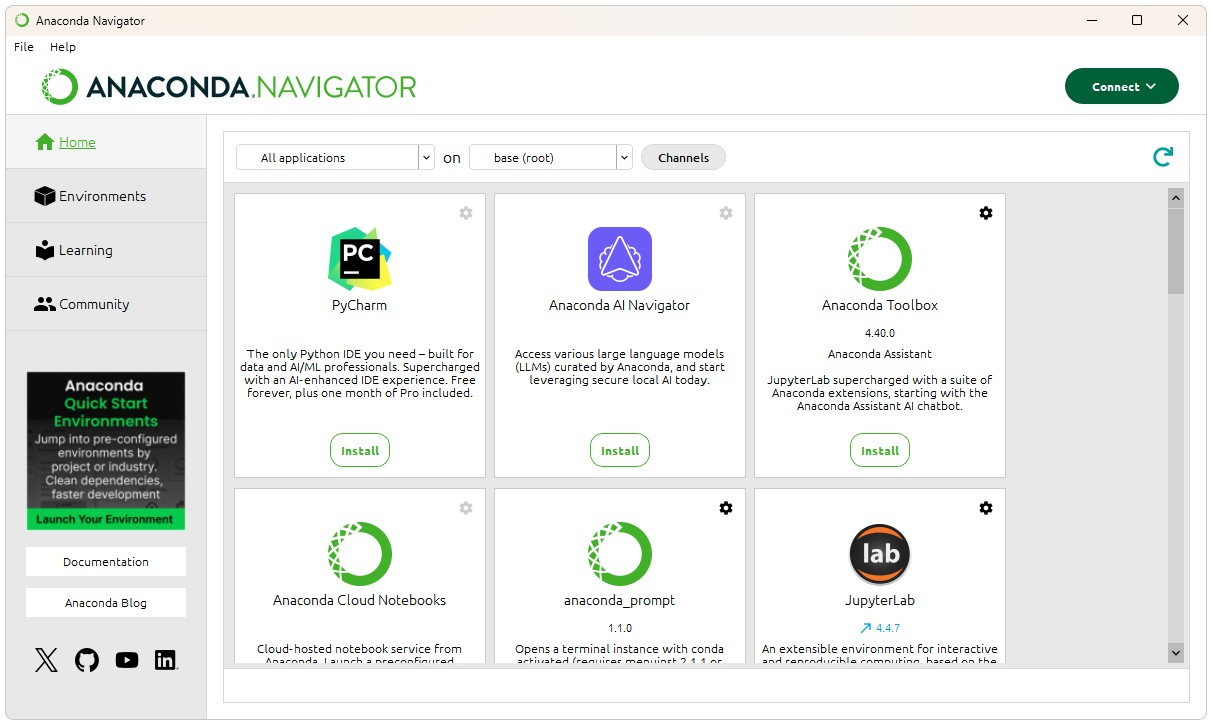
\includegraphics[width=8.33333in,height=\textheight,keepaspectratio]{images/anaconda_navigator.jpg}

}

\caption{\label{fig-anaconda3}Tela inicial do Anaconda Navigator.
Janeiro de 2026}

\end{figure}%

É possível instalar pacotes e fazer muito mais coisa diretamente pelo
Anaconda Navigator. Para os que tiverem interesse em saber um pouco
mais, esse
\href{https://www.anaconda.com/docs/getting-started/main}{link} é um bom
começo.

\subsection{IDEs}\label{ides}

Com Anaconda ou sem Anaconda, interagir diretamente com a linguagem
ainda depende do uso de um ambiente próprio para esse fim, como no caso
das chamadas IDEs. IDE é um acrônimo para Integrated Development
Environment, em português, Ambiente de Desenvolvimento Integrado. Ele é
um programa que reúne ferramentas necessárias para a construção de
outros softwares. A utilização de um IDE ajuda muito os programadores e
empresas, pois torna mais rápido o desenvolvimento de aplicações,
aumentando a produtividade e reduzindo custos. Existem IDE's específicas
para plataformas, e outras que são mais flexíveis. As mais famosas são o
Sublime Text e o Visual Studio Code.

Quais são os componentes típicos de uma IDE?

\begin{itemize}
\item
  \textbf{Editor de código-fonte}: Permite edição do código nas
  linguagens de programação suportadas pelo IDE.
\item
  \textbf{Preenchimento inteligente}: Esse é um recurso trazido pelos
  IDEs que agiliza o desenvolvimento, pois escreve automaticamente
  trechos do código como, por exemplo, comandos de função.
\item
  \textbf{Compilador}: O compilador que você escreveu em uma determinada
  linguagem de programação para a linguagem de máquina, de modo que os
  computadores o entendam.
\item
  \textbf{Debugger}: É outra ferramenta que contribui para no
  código-fonte, melhorando o desempenho do programa.
\item
  \textbf{Geração de código}: Com esse recurso, é possível predefinir
  trechos de códigos para serem usados de modelo em outros projetos,
  agilizando o desenvolvimento de trabalhos futuros.
\end{itemize}

Como podemos ver, os IDEs reúnem diversas ferramentas que tornam mais
simples a vida dos programadores. Dentre todos os benefícios que a
utilização desses programas pode trazer para seus projetos, podemos
citar alguns:

\begin{itemize}
\tightlist
\item
  Reduz o tempo gasto em cada aplicação;
\item
  Permite o desenvolvimento de um código mais limpo, organizado e
  legível;
\item
  Aumenta a produtividade dos desenvolvedores e das empresas;
\item
  Reduz a quantidade de bugs e falhas no código-fonte;
\item
  Reúne diversas ferramentas em um só lugar.
\end{itemize}

\subsubsection{Spyder}\label{spyder}

O Spyder é uma ferramenta leve, simples e ao mesmo tempo poderosa. É um
IDE Python de código aberto que conta com elementos avançados de edição,
depuração e testes interativos. Ele é bastante utilizado para o
aprendizado de Data Science, apesar de não fornecer ferramentas tão
avançadas nesse sentido como outras disponíveis. Mas ele é prático e seu
depurador destaca bem funções, variáveis e erros. Conta também com um
recurso de exploração de variáveis, que exibe os conteúdos armazenados
dentro de cada uma. Isso poupa a escrita de comandos de impressão de
variáveis na tela.

Disponível com a instalação do
\href{https://www.anaconda.com/products/distribution}{Anaconda}, uma das
maiores e mais utilizadas plataformas de distribuição do Python.

\subsubsection{Jupyter}\label{jupyter}

É um IDE Python gratuito, utilizado principalmente na análise e ciência
de dados. Ele é fácil e intuitivo, proporcionando um bom ambiente para
iniciantes em Python. Também conta com muitos materiais de referência,
tornando-se um dos IDEs mais utilizados pela comunidade. Ele trabalha
muito bem com grandes conjuntos de dados. Além disso, é ótimo para a
estética do código e atua como uma. É possível visualizar e editar
facilmente seu código para deixá-lo mais atraente e apresentável.

Além de tudo isso, a estrutura do Jupyter serve muito ao propósito de
tornar o código mais facilmente replicável, já que é possível intercalar
células de comentários e explicações em linguagem Markdown com células
de código propriamente dito, seguidas do resultado (ou erros) das
instruções. Ele possui ainda integrações com HTML, por exemplo, que
fazem a diferença principalmente na hora de apresentar projetos ou
utilizá-los para o aprendizado. O material aula a aula do nosso curso,
por exemplo, foi inteiramente desenvolvido e criado no Jupyter!

\subsubsection{Google Colaboratory}\label{google-colaboratory}

O \href{https://colab.research.google.com/notebooks/intro.ipynb}{Google
Colaboratory}, carinhosamente chamado de Colab, é um serviço de nuvem
gratuito hospedado pelo próprio Google para incentivar a pesquisa de
Aprendizado de Máquina e Inteligência Artificial.

É uma ferramenta que permite que você misture código fonte (geralmente
em python) e texto rico (geralmente em markdown) com imagens e o
resultado desse código, assim como o próprio Jupyter e sua estrutura de
\emph{notebooks} (``cadernos'' em inglês). Uma diferença importante é
que no caso do Colab os recursos computacionais utilizados para a
execução do código são os da Google e não do seu computador. Apesar da
versão gratuita disponibilizar apenas algo como 12GB de RAM, é possível
ampliar essa capacidade de processamento da máquina virtual por uma
conta paga que começa em \$5 mensais.

\section{Construindo o primeiro
programa}\label{construindo-o-primeiro-programa}

Uma vez entendido o papel do ambiente de programação, o próximo passo é
escrever e executar instruções simples. Isso permite observar
diretamente como o Python interpreta o código e produz resultados,
estabelecendo a base para todo o restante do curso. Tradicionalmente, o
primeiro programa que se escreve em uma nova linguagem chama-se
\emph{``Hello, World!''}, porque tudo o que faz é exibir as palavras
\emph{``Hello, World!''} na tela. No Python, ele se parece com isto:

\begin{Shaded}
\begin{Highlighting}[]
\BuiltInTok{print}\NormalTok{(}\StringTok{\textquotesingle{}Hello, World!\textquotesingle{}}\NormalTok{)}
\end{Highlighting}
\end{Shaded}

\begin{verbatim}
Hello, World!
\end{verbatim}

Este é um exemplo de uma instrução print (instrução de impressão),
embora na realidade ela não imprima nada em papel. Ela exibe um
resultado na tela. As aspas apenas marcam o começo e o fim do texto a
ser exibido; elas não aparecem no resultado. Os parênteses indicam que o
print é uma função.

\subsection{Operadores aritméticos}\label{operadores-aritmuxe9ticos}

Depois do \emph{``Hello, World''}, o próximo passo natural é a
aritmética. O Python tem operadores, que são símbolos especiais
representando operações de computação, como adição e multiplicação. Os
operadores \(+\), \(-\) e \(*\) executam a adição, a subtração e a
multiplicação, Finalmente, o operador \(**\) executa a exponenciação;
isto é, eleva um número a uma potência, como nos seguintes exemplos:

\begin{Shaded}
\begin{Highlighting}[]
\DecValTok{40} \OperatorTok{+} \DecValTok{2}
\end{Highlighting}
\end{Shaded}

\begin{verbatim}
42
\end{verbatim}

\begin{Shaded}
\begin{Highlighting}[]
\DecValTok{43} \OperatorTok{{-}} \DecValTok{1}
\end{Highlighting}
\end{Shaded}

\begin{verbatim}
42
\end{verbatim}

\begin{Shaded}
\begin{Highlighting}[]
\DecValTok{6} \OperatorTok{*} \DecValTok{7}
\end{Highlighting}
\end{Shaded}

\begin{verbatim}
42
\end{verbatim}

\begin{Shaded}
\begin{Highlighting}[]
\DecValTok{84} \OperatorTok{/} \DecValTok{2}
\end{Highlighting}
\end{Shaded}

\begin{verbatim}
42.0
\end{verbatim}

\begin{Shaded}
\begin{Highlighting}[]
\DecValTok{6} \OperatorTok{**} \DecValTok{2} \OperatorTok{+} \DecValTok{6}
\end{Highlighting}
\end{Shaded}

\begin{verbatim}
42
\end{verbatim}

Em algumas outras linguagens, o \(^\) é usado para a exponenciação, mas
no Python é um operador \emph{bitwise}, chamado XOR. Se não tiver
familiaridade com operadores bitwise, o resultado o surpreenderá. Não
abordaremos operadores bitwise neste curso, mas você pode ler sobre eles
em http://wiki.python.org/moin/BitwiseOperators.

\begin{Shaded}
\begin{Highlighting}[]
\DecValTok{6} \OperatorTok{\^{}} \DecValTok{2}
\end{Highlighting}
\end{Shaded}

\begin{verbatim}
4
\end{verbatim}

\subsection{Instruções e
variáveis}\label{instruuxe7uxf5es-e-variuxe1veis}

Uma instrução é uma unidade básica de código que produz algum efeito,
como criar uma variável ou exibir um valor na tela. Entre os recursos
mais importantes de uma linguagem de programação está a possibilidade de
trabalhar com variáveis, que permitem armazenar e reutilizar informações
ao longo do código. Uma variável pode ser entendida como um nome que faz
referência a um valor. No Python, uma variável é criada por meio de uma
instrução de atribuição, feita a partir de um sinal de igual.

\begin{Shaded}
\begin{Highlighting}[]
\NormalTok{message }\OperatorTok{=} \StringTok{\textquotesingle{}And now for something completely different\textquotesingle{}}
\NormalTok{n }\OperatorTok{=} \DecValTok{17}
\NormalTok{pi }\OperatorTok{=} \FloatTok{3.141592653589793}
\end{Highlighting}
\end{Shaded}

Esse exemplo faz três atribuições. A primeira atribui uma string a uma
nova variável chamada \texttt{message}; a segunda dá o número inteiro
\(17\) a \texttt{n}; a terceira atribui o valor (aproximado) de \(\pi\)
a \texttt{pi}. Uma vez definida, você pode chamar a variável e fazer
operações com o valor a ela atribuído apenas referenciando o seu nome.

\begin{Shaded}
\begin{Highlighting}[]
\NormalTok{n }\OperatorTok{+} \DecValTok{25}
\end{Highlighting}
\end{Shaded}

\begin{verbatim}
42
\end{verbatim}

\begin{Shaded}
\begin{Highlighting}[]
\NormalTok{z }\OperatorTok{=}\NormalTok{ n}\OperatorTok{*}\DecValTok{2} \OperatorTok{+} \DecValTok{16}
\BuiltInTok{print}\NormalTok{(z)}
\end{Highlighting}
\end{Shaded}

\begin{verbatim}
50
\end{verbatim}

Os programadores geralmente escolhem nomes significativos para as suas
variáveis -- eles documentam o uso da variável. Nomes de variáveis podem
ser tão longos quanto você queira. Podem conter tanto letras como
números, mas não podem começar com um número. O caractere de sublinhar
(\_) pode aparecer em um nome. Muitas vezes é usado em nomes com várias
palavras, como \emph{full\_name}.

Se você der um nome ilegal a uma variável, recebe um erro de sintaxe:

\begin{Shaded}
\begin{Highlighting}[]
\DecValTok{76}\ErrorTok{trombones} \OperatorTok{=} \StringTok{\textquotesingle{}big parade\textquotesingle{}}
\end{Highlighting}
\end{Shaded}

\begin{Highlighting}
\textcolor{black}{SyntaxError: invalid decimal literal (3381618747.py, line 1)}
\textcolor{black}{  }\textcolor{QuartoInternalColor1}{Cell}\textcolor{QuartoInternalColor2}{}\textcolor{QuartoInternalColor1}{ }\textcolor{QuartoInternalColor2}{}\textcolor{QuartoInternalColor3}{In[11]}\textcolor{QuartoInternalColor2}{}\textcolor{QuartoInternalColor3}{, line 1}\textcolor{QuartoInternalColor2}{}
\textcolor{QuartoInternalColor2}{}\textcolor{QuartoInternalColor4}{    }\textcolor{QuartoInternalColor2}{}\textcolor{QuartoInternalColor4}{76trombones = 'big parade'}\textcolor{QuartoInternalColor2}{}
\textcolor{QuartoInternalColor2}{     \textasciicaret{}}
\textcolor{QuartoInternalColor2}{}\textcolor{QuartoInternalColor4}{SyntaxError}\textcolor{QuartoInternalColor2}{}\textcolor{QuartoInternalColor4}{:}\textcolor{QuartoInternalColor2}{ invalid decimal literal}
\end{Highlighting}

\begin{Shaded}
\begin{Highlighting}[]
\KeywordTok{class} \OperatorTok{=} \StringTok{\textquotesingle{}Advanced Theoretical Zymurgy\textquotesingle{}}
\end{Highlighting}
\end{Shaded}

\begin{Highlighting}
\textcolor{black}{SyntaxError: invalid syntax (3803549429.py, line 1)}
\textcolor{black}{  }\textcolor{QuartoInternalColor1}{Cell}\textcolor{QuartoInternalColor2}{}\textcolor{QuartoInternalColor1}{ }\textcolor{QuartoInternalColor2}{}\textcolor{QuartoInternalColor3}{In[12]}\textcolor{QuartoInternalColor2}{}\textcolor{QuartoInternalColor3}{, line 1}\textcolor{QuartoInternalColor2}{}
\textcolor{QuartoInternalColor2}{}\textcolor{QuartoInternalColor4}{    }\textcolor{QuartoInternalColor2}{}\textcolor{QuartoInternalColor4}{class = 'Advanced Theoretical Zymurgy'}\textcolor{QuartoInternalColor2}{}
\textcolor{QuartoInternalColor2}{          \textasciicaret{}}
\textcolor{QuartoInternalColor2}{}\textcolor{QuartoInternalColor4}{SyntaxError}\textcolor{QuartoInternalColor2}{}\textcolor{QuartoInternalColor4}{:}\textcolor{QuartoInternalColor2}{ invalid syntax}
\end{Highlighting}

\texttt{76trombones} é ilegal porque começa com um número. Mas o que há
de errado com \texttt{class}?

A questão é que class é uma das palavras-chave do Python. O
interpretador usa palavras-chave para reconhecer a estrutura do programa
e elas não podem ser usadas como nomes de variável. O Python 3 tem estas
palavras-chave:

\begin{Shaded}
\begin{Highlighting}[]
\KeywordTok{and}         \KeywordTok{del}         \ImportTok{from}        \VariableTok{None}        \VariableTok{True}
\ImportTok{as}          \ControlFlowTok{elif}        \KeywordTok{global}      \KeywordTok{nonlocal}    \ControlFlowTok{try}
\ControlFlowTok{assert}      \ControlFlowTok{else}        \ControlFlowTok{if}          \KeywordTok{not}         \ControlFlowTok{while}
\ControlFlowTok{break}       \ControlFlowTok{except}      \ImportTok{import}      \KeywordTok{or}          \ControlFlowTok{with}
\KeywordTok{class}       \VariableTok{False}       \KeywordTok{in}          \ControlFlowTok{pass}        \ControlFlowTok{yield}
\ControlFlowTok{continue}    \ControlFlowTok{finally}     \KeywordTok{is}          \ControlFlowTok{raise}
\KeywordTok{def}         \ControlFlowTok{for}         \KeywordTok{lambda}      \ControlFlowTok{return}
\end{Highlighting}
\end{Shaded}

Você não precisa memorizar essa lista. Na maior parte dos ambientes de
desenvolvimento, as palavras-chave são exibidas em uma cor diferente; se
você tentar usar uma como nome de variável, vai perceber.

\subsection{Leitura de erros}\label{leitura-de-erros}

Você viu anteriormente que quando o Python se depara com algum erro no
código ele interrompe a execução e exibe uma mensagem de erro. Essa
mensagem não é aleatória: ela segue uma estrutura relativamente
padronizada e contém informações úteis para diagnosticar o que
aconteceu. De forma geral, uma mensagem de erro em Python possui três
componentes principais:

\begin{enumerate}
\def\labelenumi{\arabic{enumi}.}
\tightlist
\item
  \textbf{O tipo do erro}. Indica a natureza do problema (por exemplo,
  \texttt{SyntaxError}, \texttt{NameError}, \texttt{TypeError}). Esse é
  o ponto de partida para entender que tipo de falha ocorreu.
\item
  \textbf{A descrição do erro}. Uma frase curta que detalha o problema
  detectado pelo interpretador, como \emph{``invalid syntax''} ou
  \emph{``name is not defined''}.
\item
  \textbf{A localização do erro}. Normalmente inclui o arquivo, a linha
  do código e, em alguns casos, um indicador visual apontando o ponto
  exato onde o Python identificou o problema.
\end{enumerate}

Considere o seguinte exemplo:

\begin{Shaded}
\begin{Highlighting}[]
\BuiltInTok{print}\NormalTok{(}\StringTok{"Olá mundo"}
\end{Highlighting}
\end{Shaded}

\begin{Highlighting}
\textcolor{black}{\_IncompleteInputError: incomplete input (2274650354.py, line 1)}
\textcolor{black}{  }\textcolor{QuartoInternalColor1}{Cell}\textcolor{QuartoInternalColor2}{}\textcolor{QuartoInternalColor1}{ }\textcolor{QuartoInternalColor2}{}\textcolor{QuartoInternalColor3}{In[13]}\textcolor{QuartoInternalColor2}{}\textcolor{QuartoInternalColor3}{, line 1}\textcolor{QuartoInternalColor2}{}
\textcolor{QuartoInternalColor2}{}\textcolor{QuartoInternalColor4}{    }\textcolor{QuartoInternalColor2}{}\textcolor{QuartoInternalColor4}{print("Olá mundo"}\textcolor{QuartoInternalColor2}{}
\textcolor{QuartoInternalColor2}{                     \textasciicaret{}}
\textcolor{QuartoInternalColor2}{}\textcolor{QuartoInternalColor4}{\_IncompleteInputError}\textcolor{QuartoInternalColor2}{}\textcolor{QuartoInternalColor4}{:}\textcolor{QuartoInternalColor2}{ incomplete input}
\end{Highlighting}

Ao executar esse código, o Python retorna um erro do tipo
\texttt{\_IncompleteInputError}. Logo após o tipo há uma breve descrição
do erro, que nesse caso é \texttt{incomplete\ input}. Isso ocorre porque
o parêntese de fechamento está ausente, tornando o código inválido do
ponto de vista da linguagem. A própria mensagem de erro replica a linha
de código com problema e indica a posição em que há o problema de
sintaxe. Com o tempo, esse processo de indentificar o tipo, entender o
erro para além do tipo e a provável localização no código torna-se quase
automático. A habilidade de interpretar mensagens de erro é uma das
competências mais importantes em programação e será exercitada
continuamente ao longo do curso.

\section{Pacotes de terceiros e funções
não-nativas}\label{pacotes-de-terceiros-e-funuxe7uxf5es-nuxe3o-nativas}

\subsection{Como instalar}\label{como-instalar-1}

Para instalar novos pacotes para o Python precisamos fazê-lo via prompt
de comando. O Anaconda nos fornece um prompt de comando próprio, o
\textbf{Anaconda Prompt} que facilita a instalação desses pacotes
através dos comandos \texttt{conda} ou \texttt{pip}. Vamos instalar como
exemplo o pacote
\href{https://github.com/tqdm/tqdm\#installation}{\texttt{tqdm}}, que
nos permite criar barras de progresso em atividades repetidas.

\begin{enumerate}
\def\labelenumi{\arabic{enumi}.}
\tightlist
\item
  Abra o \textbf{Anaconda prompt}.
\item
  Veja se o pacote já não está instalado: digite \texttt{conda\ list}.
\item
  Você pode utilizar 2 comandos distintos para instalar o pacote:
  \texttt{conda\ install\ tqdm} ou \texttt{pip\ install\ tqdm}.
\end{enumerate}

Note também que alguns dos principais pacotes sobre os quais falarei ao
longo do curso, \emph{NumPy, SciPy, Matplotlib e Pandas}, já vem
instalados com o Anaconda, o que não é verdade no Python puro. Mais do
que mostrar o que temos instalado na nossa máquina local, o comando
\texttt{conda\ list} nos mostra as versões de cada uma das bibliotecas
disponíveis e qual o ambiente utilizado em sua instalação.

\textbf{Diferença entre \emph{conda} e \emph{pip}}: falar mais sobre a
diferença entre esses dois comandos populares para instalação de pacotes
vai um pouco além do escopo desse curso. De forma bastante resumida,
podemos dizer que o \texttt{pip} é um gerenciador de pacotes que nos
permite instalar qualquer biblioteca escrita em Python e disponível no
\emph{Python Package Index} (PyPI), o principal repositório de pacotes
para a linguagem. O \texttt{conda}, no entanto, é mais do que um simples
gerenciador de pacotes já que é possível fazer diferentes instalações em
diferentes ambientes de modo a reduzir problemas de incompatibilidade
entre versões. Além disso, através do \texttt{conda} podemos instalar
pacotes escritos em outras linguagens também, como R e C++. Por outro
lado, é possível que você demore mais e tenha problemas para instalar
alguns pacotes utilizando o \texttt{conda}. Aos que quiserem saber um
pouco mais sobre a diferença entre esses dois métodos para instalação,
esses links
(\href{https://www.anaconda.com/blog/understanding-conda-and-pip}{1} e
\href{https://pythonspeed.com/articles/conda-vs-pip/}{2}) podem ser um
bom começo.

\subsection{Como importar}\label{como-importar}

Sempre que quisermos trazer algo ``de fora'', devemos carregar as
bibliotecas específicas, seja por completo ou apenas um subconjunto de
suas funções. Fazemos isso por meio do comando \texttt{import}. Vamos
utilizar como exemplo a biblioteca \texttt{NumPy}, uma das principais
bibliotecas de comando do Python em se tratando de operações algébricas
e matriciais.

Dedicaremos uma aula inteira para trabalhar com o \texttt{NumPy} daqui
algumas semanas, mas por hora trabalharemos apenas com as funções
geradoras de números aleatórios, em especial a função geradora de
números aleatórios distribuídos de acordo com uma Distribuição Uniforme
padrão (vocês devem se lembrar das características dessa distribuição
das aulas de estatística, mas caso ainda restem dúvidas sempre existe o
\href{https://pt.wikipedia.org/wiki/Distribui\%C3\%A7\%C3\%A3o_uniforme}{Wikipedia}).

Há 3 formas de trabalhar com essa função específica, contida no
\texttt{NumPy}:

\begin{enumerate}
\def\labelenumi{\arabic{enumi}.}
\tightlist
\item
  Podemos importar a biblioteca inteira
\end{enumerate}

\begin{Shaded}
\begin{Highlighting}[]
\ImportTok{import}\NormalTok{ numpy}
\end{Highlighting}
\end{Shaded}

\begin{enumerate}
\def\labelenumi{\arabic{enumi}.}
\setcounter{enumi}{1}
\tightlist
\item
  Podemos importar a biblioteca inteira mas dando-lhe um ``apelido''
\end{enumerate}

\begin{Shaded}
\begin{Highlighting}[]
\ImportTok{import}\NormalTok{ numpy }\ImportTok{as}\NormalTok{ np}
\end{Highlighting}
\end{Shaded}

\begin{enumerate}
\def\labelenumi{\arabic{enumi}.}
\setcounter{enumi}{2}
\tightlist
\item
  Podemos importar apenas a função que nos interessa nesse caso
\end{enumerate}

\begin{Shaded}
\begin{Highlighting}[]
\ImportTok{from}\NormalTok{ numpy.random }\ImportTok{import}\NormalTok{ uniform}
\end{Highlighting}
\end{Shaded}

Qual a diferença entre esses métodos? No Python, sempre que formos
utilizar uma função de algum pacote ``de fora'' é preciso dizer ao
Python de onde que essa função está vindo. Se quisermos usar a função
\texttt{uniform()} através do 1º método, por exemplo, é preciso chamá-la
utilizando o nome do pacote, nesse caso \texttt{numpy.random.uniform()}.
O 2º método encurta esse nome de tal forma que é possível chamar a mesma
função usando \texttt{np.random.uniform()}. Por fim, no 3º caso basta
chamar a função diretamente, isto é, \texttt{uniform()}.

Mas se o 3º caso é mais direto, porque não usá-lo sempre? Por duas
razões bem simples: (i) usar a sintaxe dos 2 primeiros casos torna o
código mais compreensível e depurável, já que no caso de algum problema
de execução sabemos onde procurar a resposta, e (ii) é comum pacotes
distintos usarem o mesmo nome para funções que fazem operações
distintas, o que pode gerar problemas de incompatibilidade e/ou de
executarmos algo diferente daquilo que gostaríamos de executar.

Na maioria das vezes, acabamos utilizando o 2º método, já que isso
permite reduzir linhas desnecessárias de código ao mesmo tempo que
facilita a replicabilidade e a atividade de depuração do código.

\section{Conclusão}\label{conclusuxe3o-1}

Neste capítulo, você aprendeu a executar seus primeiros comandos em
Python, a interagir com o ambiente de programação e a interpretar
mensagens básicas de erro. Mais importante do que os comandos
específicos é o desenvolvimento de uma postura adequada frente ao
código: testar, observar, errar, corrigir e testar novamente. Nos
próximos capítulos, introduziremos objetos básicos da linguagem, como
números, textos e listas, sempre construindo sobre as habilidades
operacionais estabelecidas aqui.

\section{Exercícios}\label{exercuxedcios-1}

\begin{enumerate}
\def\labelenumi{\arabic{enumi}.}
\item
  Utilize o Python para responder as seguintes perguntas:

  \begin{enumerate}
  \def\labelenumii{\alph{enumii}.}
  \tightlist
  \item
    Quantos segundos há em 42 minutos e 42 segundos?
  \item
    Quantas milhas há em 10 quilômetros? Dica: uma milha equivale a 1,61
    quilômetro.
  \item
    Se você correr 10 quilômetros em 42 minutos e 42 segundos, qual é o
    \_pace\_\_ médio (tempo por quilômetro em minutos e segundos)?
  \end{enumerate}
\item
  Crie uma variável chamada \texttt{salario\_mensal} com valor igual a
  \(3500\).

  \begin{enumerate}
  \def\labelenumii{\alph{enumii}.}
  \tightlist
  \item
    Crie uma variável chamada \texttt{rendimento\_anual} que seja
    construída a partir de \texttt{salario\_mensal} e considere o
    recebimento do 13º salário no mês de dezembro. Utilize uma instrução
    para exibir \texttt{rendimento\_anual} na tela.
  \item
    Calcule e exiba na tela o valor do rendimento anual após o pagamento
    de impostos, considerando a incidência de uma alíquota média de
    \(16.5\%\).
  \end{enumerate}
\item
  Explique, com suas próprias palavras, a diferença entre escrever
  código em um editor de texto simples e escrever código em uma IDE ou
  ambiente interativo. Sua resposta deve mencionar pelo menos dois
  recursos que facilitam o aprendizado em IDEs.
\item
  Considere o código abaixo:

\begin{Shaded}
\begin{Highlighting}[]
\BuiltInTok{print}\NormalTok{(}\StringTok{"Resultado:"}
\NormalTok{resultado }\OperatorTok{==} \DecValTok{10} \OperatorTok{+} \DecValTok{5}
\end{Highlighting}
\end{Shaded}

  \begin{enumerate}
  \def\labelenumii{\alph{enumii}.}
  \tightlist
  \item
    Execute o código e identifique o tipo e posição do(s) erro(s) no
    código.
  \item
    Explique com suas palavras o que está de errado.
  \item
    Corrija o(s) erro(s) e execute novamente.
  \end{enumerate}
\end{enumerate}

\chapter{Programação e IA}\label{sec-inteligencia_artificial}

\section{Introdução}\label{introduuxe7uxe3o-2}

A incorporação recente de ferramentas de inteligência artificial ao
desenvolvimento de software alterou significativamente a forma como
programas são escritos, depurados e documentados. Em particular, modelos
de linguagem treinados em grandes volumes de código passaram a ser
capazes de gerar trechos de programas, explicar erros e sugerir soluções
alternativas de forma quase imediata.

Neste curso, a inteligência artificial não será tratada como um atalho
para ``pular'' a aprendizagem de programação, mas como um instrumento
complementar. O objetivo é utilizá-la para apoiar o entendimento da
sintaxe, acelerar tarefas mecânicas e auxiliar na identificação de
erros, sempre preservando o domínio conceitual do código pelo aluno.

\begin{figure}

\centering{

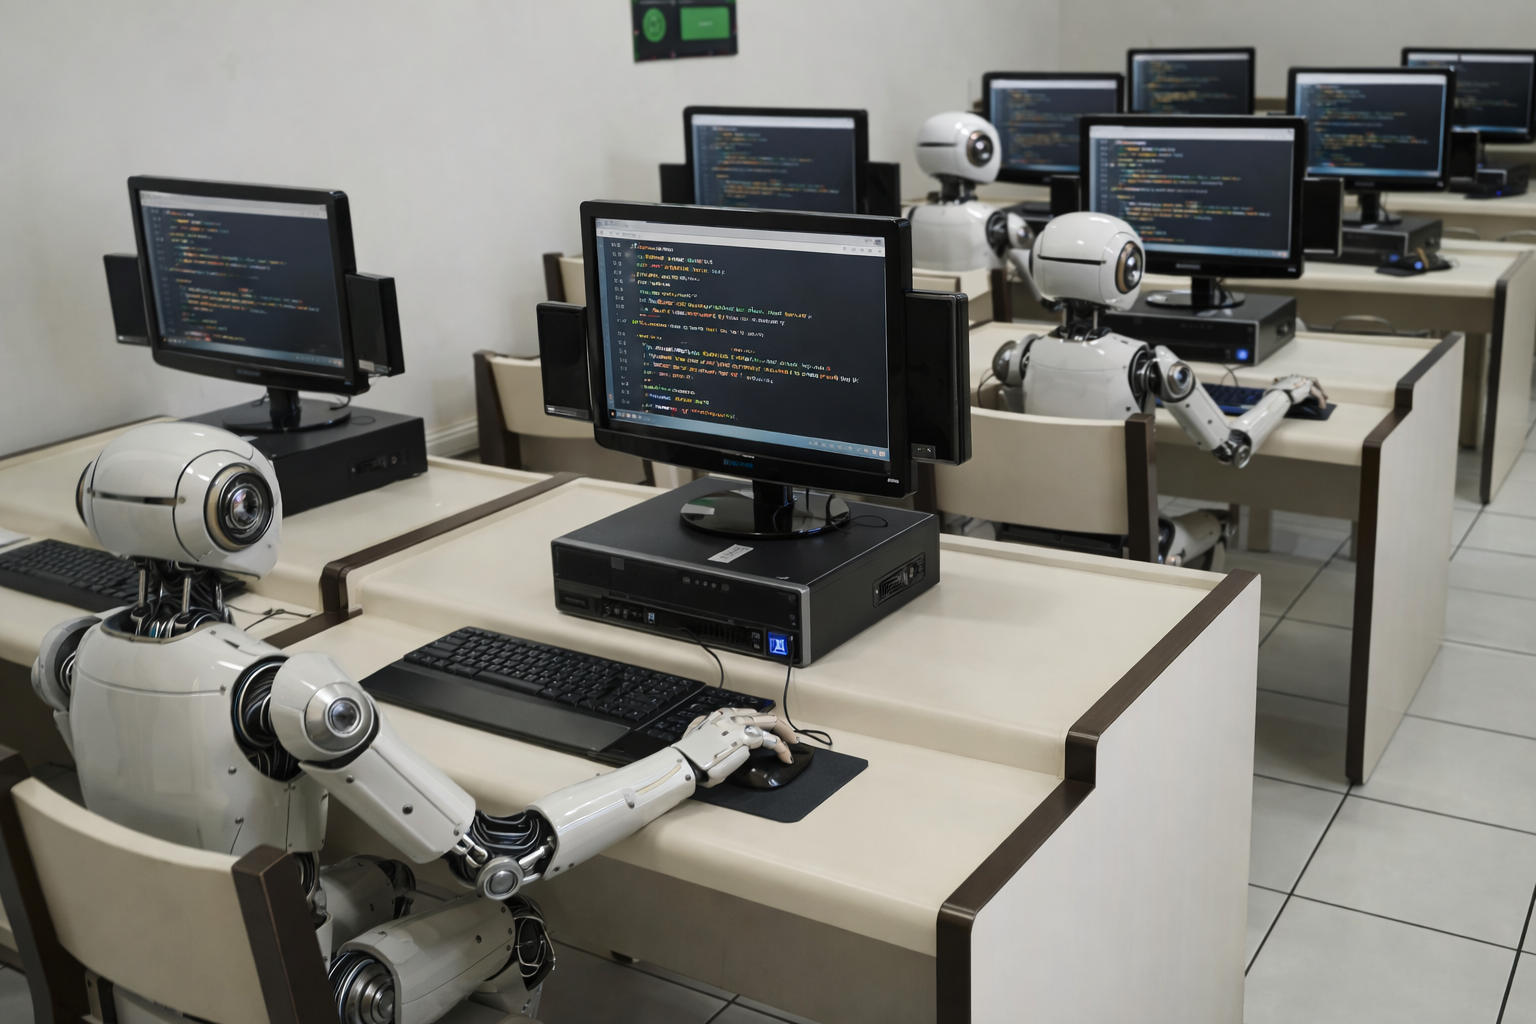
\includegraphics[width=8.33333in,height=\textheight,keepaspectratio]{images/IA.png}

}

\caption{\label{fig-ia}Turma de EAE1106 do primeiro semestre de 2072.
Imagem criada por IA.}

\end{figure}%

Antes de discutir como usar essas ferramentas de forma produtiva, é
necessário definir IA e aprender como acessar seus recursos. Só então
podemos avançar para entender o que a IA faz bem, o que faz mal e quais
riscos surgem quando ela é usada sem critério, especialmente em um
contexto de formação em métodos computacionais.

\subsection{Pré-requisitos}\label{pruxe9-requisitos-2}

Este foi escrito para que o aluno que acompanhou e absorveu o conteúdo
do dois capítulos anteriores seja plenamente capaz de acompanhar. Não há
outros pré-requisitos.

\section{O que é Inteligência
Artificial?}\label{o-que-uxe9-inteliguxeancia-artificial}

Definir IA é uma tarefa difícil, já que se trata de uma área da ciência
da computação bastante ampla que, a depender do contexto, envolve um
conjunto de modelos e aplicações diferentes. Em todos os casos, porém, é
uma área responsável por criar sistemas capazes de executar tarefas que
requerem inteligência humana, como aprendizado, raciocínio,
reconhecimento de padrões, processamento de áudio, vídeo e linguagem.
Esses sistemas são construídos à partir de uma grande amostra de dados,
nos quais diferentes modelos são treinados e à partir dos quais é
possível construir previsões e análises sobre conjuntos de dados novos.
Podemos citar alguns exemplos que, em geral, são aplicações de sistemas
de IA: sistemas de recomendação, robótica, diagnóstico médico, sistema
de previsão, automação.

Embora se discuta Inteligência Artificial há algum tempo, apenas mais
recentemente a chamada Inteligência Artificial Generativa (IAG) ganhou
espaço no debate e nos modelos de uso comercial. Diferentemente dos
algoritmos mais gerais de inteligência artificial, os modelos de IAG são
projetados para a criação de algo novo, que não estava presente nos
dados originais. Em essência, os sistemas de IAG são sistemas de IA com
um escopo mais restrito e bem definido.

No mundo da programação, ferramentas de IAG são especialmente eficazes
em tarefas como escrever estruturas sintáticas comuns, explicar
mensagens de erro frequentes ou converter descrições em linguagem
natural para código simples. Essas características fazem com que a IAG
seja útil como um assistente de programação, semelhante a um monitor
humano muito rápido. No entanto, modelos como o ChatGPT não ``sabem''
programação no sentido humano. Eles operam prevendo sequências de texto
com base em padrões estatísticos aprendidos durante a fase de
treinamento do modelo. Isso significa que essas ferramentas podem
produzir respostas plausíveis, mas não necessariamente verdadeiras. Além
disso, a IAG não conhece a sequência didática adotada e não distingue
soluções apropriadas de soluções excessivamente complexas para o nível
do aluno. Por esse motivo, o uso indiscriminado dessas ferramentas pode
gerar dependência, dificultar a internalização de conceitos básicos como
tipos de dados, controle de fluxo e escopo de variáveis.

\section{\texorpdfstring{\emph{Large Language Models
(LLMs)}}{Large Language Models (LLMs)}}\label{large-language-models-llms}

Dentro do grupo de modelos de IAG estão os famosos GPTs, como o
\href{https://chatgpt.com/}{ChatGPT} e o
\href{https://gemini.google.com/}{Gemini}. Os GPTs são modelos da classe
dos \emph{Large Language Models}, que compreendem e geram conteúdo
textual novo com base em uma etapa de pré-treino em grande volume de
textos. Nesses modelos, o sistema recebe uma mensagem (prompt) de
entrada, ``raciocina'' em cima do texto fornecido e dos dados nos quais
foi pré-treinado, e retorna uma mensagem de saída em resposta. É como se
o modelo tivesse por objetivo prever a próxima palavra (ou token) em um
texto, dadas as palavras anteriores. Quando aplicados a código, esses
modelos exploram regularidades presentes em milhões de exemplos de
programas escritos por humanos.

É importante destacar que, embora extremamente úteis para programação,
esses modelos:

\begin{itemize}
\tightlist
\item
  Não executam o código que geram. Eles produzem sequências de texto
  estatisticamente plausíveis.
\item
  Não verificam automaticamente se o código está correto.
\item
  Não ``sabem'' matemática, economia ou programação no sentido humano.
\item
  Por vezes tendem a escolher respostas mais complexas e complicada do
  que o necessário.
\end{itemize}

No fundo, tais modelos apenas produzem sequências plausíveis de texto
com base em padrões estatísticos. Isso explica por que respostas podem
parecer convincentes, mas conter erros lógicos, uso inadequado de
funções ou soluções incompatíveis com o nível do curso. Essa limitação
torna essencial que o aluno atue como validador ativo de qualquer
resposta produzida por IA.

\begin{tcolorbox}[enhanced jigsaw, bottomrule=.15mm, colframe=quarto-callout-note-color-frame, arc=.35mm, coltitle=black, titlerule=0mm, opacityback=0, colback=white, toptitle=1mm, breakable, bottomtitle=1mm, toprule=.15mm, left=2mm, leftrule=.75mm, title=\textcolor{quarto-callout-note-color}{\faInfo}\hspace{0.5em}{Curiosidade}, rightrule=.15mm, opacitybacktitle=0.6, colbacktitle=quarto-callout-note-color!10!white]

Você sabe o que significa GPT? É a sigla para \textbf{Generative
Pre-trained Transformer}, que resume as características dos modelos por
trás de sistemas como o ChatGPT. \emph{Generative} faz referência a
modelos de IAG, que tem como objetivo principal criar conteúdo novo a
partir de um dado conjunto de informações. \emph{Pre-trained} faz
referência ao fato do modelo ser pré-treinado em um grande volume de
dados textuais genéricos, em geral de domínio público como o Wikipedia,
até uma determinada data de corte. Por fim, \emph{Transformer} é uma
classe de modelos mais recentes, desenvolvidos inicialmente pelas
equipes de pesquisa do Google, com certas particularidades que os tornam
altamente eficientes e assertivos em tarefas que envolvem mensagens de
entrada em formato de texto.

\end{tcolorbox}

\section{ChatGPT}\label{chatgpt}

\subsection{Acesso à plataforma e primeiro
uso}\label{acesso-uxe0-plataforma-e-primeiro-uso}

O acesso à ferramenta é feito pelo \href{https://chatgpt.com/}{site} ou
pelo aplicativo móvel, disponível gratuitamente na Apple Store ou Google
Store. A plataforma se parece com um chat qualquer, assim como um
aplicativo de mensagens. A diferença é que quem responde é o próprio
modelo. Assim, para fazer algum questionamento ou pedir algum auxílio
com o seu código, por exemplo, basta digitar na caixa de entrada a
mensagem que resume aquilo que se deseja que o modelo responda. A Figura
Figura~\ref{fig-chatgpt} apresenta o layout base e como realizar uma
requisição ao ChatGPT através do website.

\begin{figure}

\begin{minipage}{\linewidth}

\pandocbounded{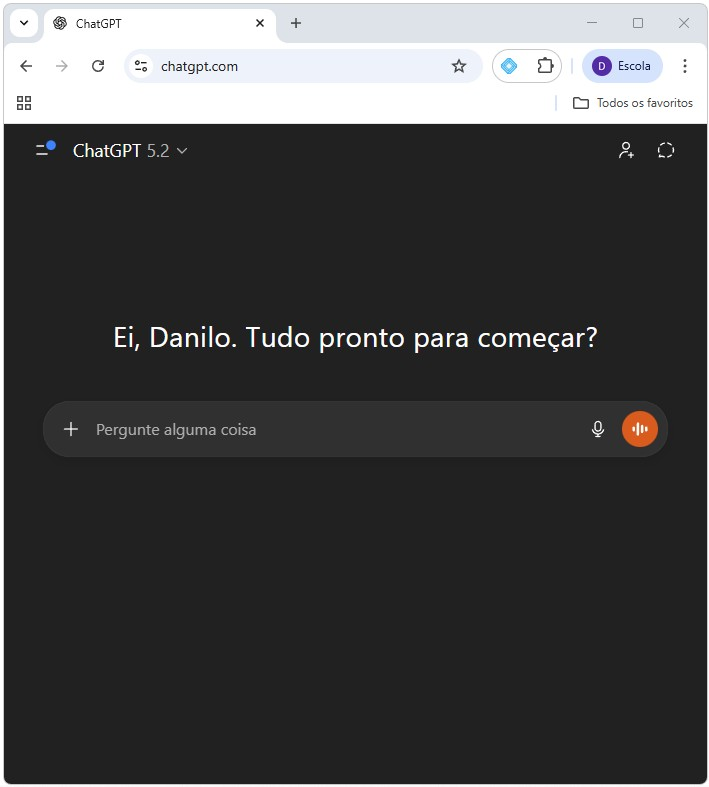
\includegraphics[keepaspectratio]{images/chatgpt1.jpg}}

\subcaption{\label{}Tela inicial}
\end{minipage}%
\newline
\begin{minipage}{\linewidth}

\pandocbounded{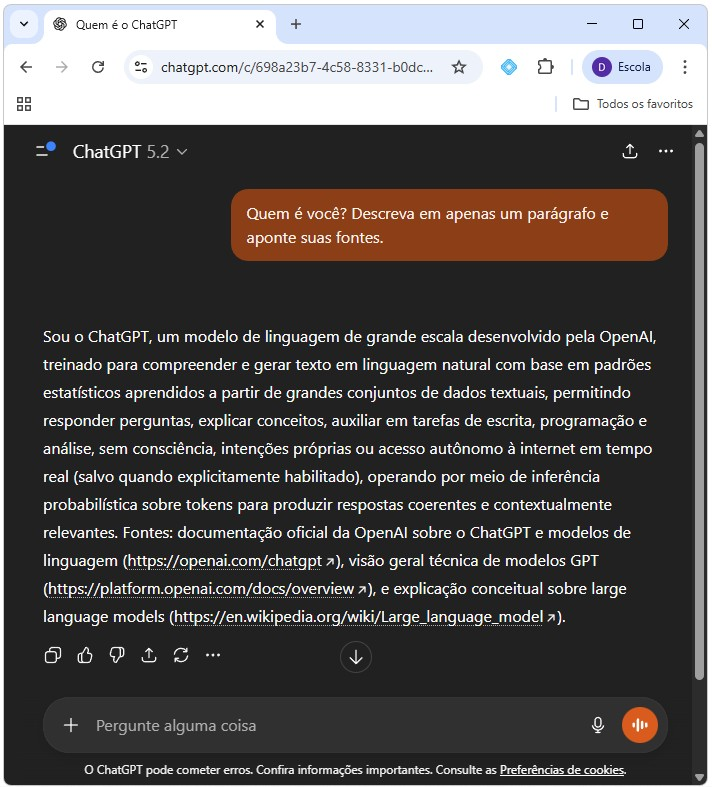
\includegraphics[keepaspectratio]{images/chatgpt2.jpg}}

\subcaption{\label{}Pergunta e resposta}
\end{minipage}%

\caption{\label{fig-chatgpt}Layout do aplicativo web do ChatGPT.
Fevereiro de 2026.}

\end{figure}%

As requisições ao modelo são gratuitas, porém, com acesso limitado às
versões mais recentes do modelo, com maior capacidade de processamento,
eficácia e assertividade nas respostas. É plenamente possível utilizar a
versão gratuita para requisições esporádicas e mais simples, que não
envolvam mídias como aúdio ou imagens. Usuários mais intensos e que
demandam respostas mais confiáveis podem se frustar com as
funcionalidades da versão gratuita. A OpenAI, empresa por trás do
ChatGPT, oferece alguns planos pagos que dão direito a uso ilimitado
dessas novas versões do modelo e outras funcionalidades.

\begin{figure}

\centering{

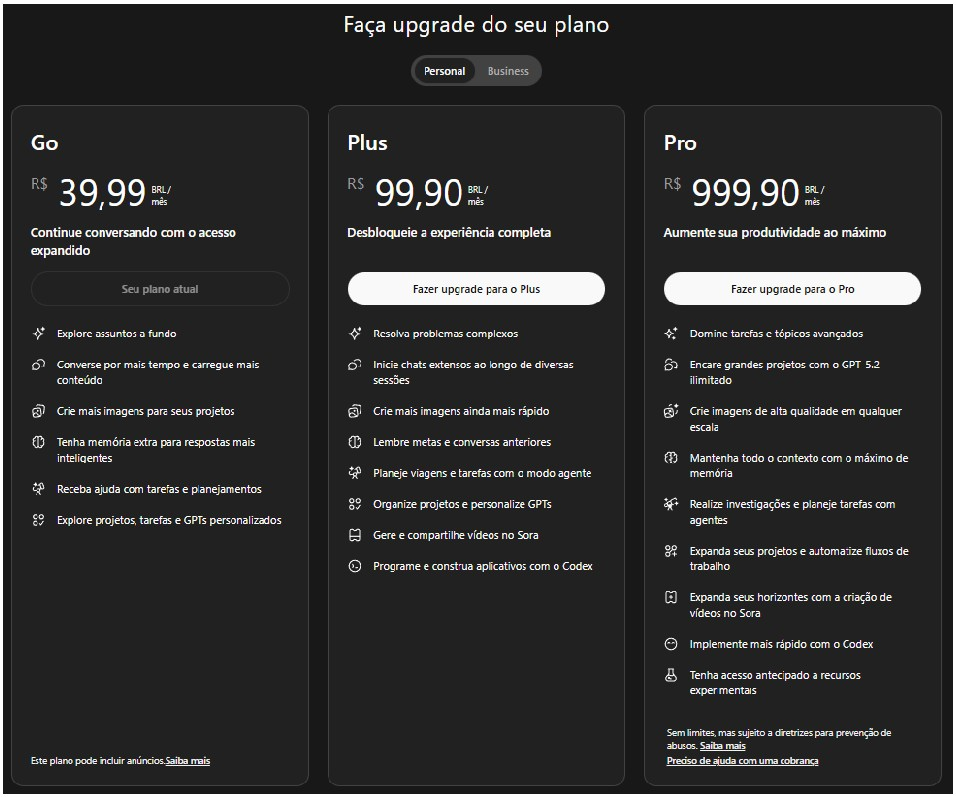
\includegraphics[width=7.29167in,height=\textheight,keepaspectratio]{images/chatgpt3.jpg}

}

\caption{\label{fig-chatgptplus}Planos e valores do ChatGPT. Fevereiro
de 2026.}

\end{figure}%

No entanto, nem sempre as ferramentas de inteligência artificial são
indicadas. Existem limitações importantes que, se não compreendidas,
podem gerar respostas pouco eficazes, incorretas e até mesmo implicar
problemas legais. Diante dessas limitações, o uso da ferramenta em
qualquer aplicação deve ser precedido por três perguntas básicas,
listadas abaixo. Se qualquer uma dessas condições não for satisfeita, o
uso da ferramenta deve ser reavaliado ou evitado.

\begin{enumerate}
\def\labelenumi{\arabic{enumi}.}
\item
  \textbf{A acurácia é um requisito central da sua aplicação?} Embora o
  modelo tenha sido treinado com bilhões de textos e conjuntos de dados,
  não há garantia de respostas \(100%
  \) corretas. Além disso, há um grau inerente de imprevisibilidade:
  pequenas variações no prompt podem gerar respostas diferentes, e o
  próprio modelo é não determinístico. Isso significa que, mesmo com a
  mesma pergunta, resultados distintos podem surgir. Para aplicações que
  exigem precisão rigorosa e consistência absoluta, essa limitação deve
  ser considerada explicitamente.
\item
  \textbf{Os resultados são verificáveis?} Ferramentas como o ChatGPT
  não substituem conhecimento humano especializado. Por serem modelos,
  podem produzir respostas semanticamente plausíveis, mas incorretas ou
  desalinhadas do objetivo pretendido. A verificação exige domínio
  mínimo do tema tratado. Como regra prática: evite solicitar algo que
  você não tenha condições de conferir, validar ou testar
  posteriormente.
\item
  \textbf{Dados da apicação são sensíveis ou protegidos?} O
  compartilhamento de dados confidenciais com ferramentas de IAG pode
  implicar riscos jurídicos e, a depender da natureza da informação,
  pode inclusive configurar infração legal. Sempre avalie cuidadosamente
  se os dados utilizados estão protegidos por normas de sigilo,
  contratos ou legislação específica antes de inseri-los em qualquer
  sistema externo.
\end{enumerate}

\includegraphics[width=8.19in,height=6.8in]{inteligencia_artificial_files/figure-latex/mermaid-figure-1.png}

\subsection{Conceitos básicos de engenharia de
prompt}\label{conceitos-buxe1sicos-de-engenharia-de-prompt}

Como você já deve ter percebido, a qualidade da resposta da ferramenta
de IAG depende fortemente da clareza, do contexto e das restrições
explícitas incluídas na instrução (ou pergunta) enviada pelo usuário,
isto é, depende da qualidade do \emph{prompt}. Prompts vagos tendem a
gerar respostas genéricas ou excessivamente complexas. Já prompts bem
formulados permitem que a IA produza respostas mais alinhadas ao
objetivo desejado.

\emph{Prompt Engineering} (ou engenharia de prompt) é o processo de
estruturar uma prompt de forma a auxiliar a compreensão dos modelos de
linguagem e ampliar a assertividade e eficiência das respostas. Apesar
de ser uma área em expansão, que conta com várias estratégias para a
construção de prompts altamente personalizados para cada aplicação, são
duas as características essenciais que devem estar presentes em todo
prompt: clareza e especificidade.

\begin{itemize}
\item
  \textbf{Clareza}: para tornar o prompt claro aos olhos do modelo, é
  preciso fornecer elementos que objetivos que auxiliem o modelo a
  fornecer respostas mais direcionadas. Para isso, é importante (i)
  descrever o contexto relevante, (ii) adicionar detalhes específicos ao
  objeto e (iii) ser preciso nas instruções.
\item
  \textbf{Especificidade}: para tornar o prompt menos genérico e melhor
  direcionar a resposta do modelo, é preciso que o foco seja apenas no
  que é mais relevante para o objetivo em questão. Prompts vagos e
  ambíguos promovem respostas menos acuradas e eficientes. Nesse caso,
  (i) seja descritivo, (ii) evite amiguidades e informações
  desnecessárias, (iii) evite dizer ao modelo o que não fazer; o foco
  deve ser em instruções do que queremos que seja feito.
\end{itemize}

No fim das contas, um bom prompt é aquele que oferece as instruções
corretas ao modelo, que então devolve a resposta esperada. Alguns
elementos ajudam nesse processo de construir um prompt mais claro e
específico: instruções, contexto, exemplos e formato de saída (Figura
Figura~\ref{fig-prompt}). Lembre, o objetivo é ser claro e específico,
orientando o modelo a responder aquilo que queremos que ele responda.

\begin{figure}

\centering{

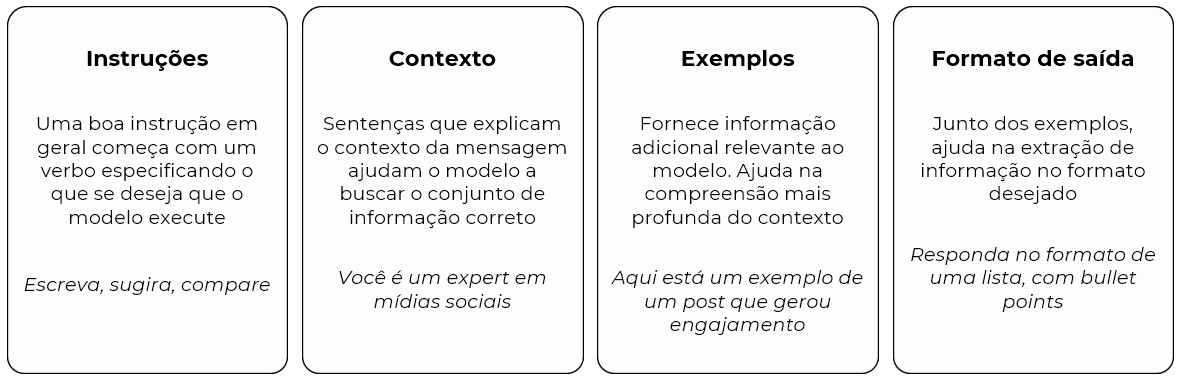
\includegraphics[width=8.33333in,height=\textheight,keepaspectratio]{images/prompts.jpg}

}

\caption{\label{fig-prompt}Elementos desejáveis dentro de um prompt}

\end{figure}%

\subsection{Exemplo de uso em
programação}\label{exemplo-de-uso-em-programauxe7uxe3o}

A melhor forma de compreender essas diretrizes é aplicá-las na prática.
A Figura Figura~\ref{fig-bhaskara} mostra o caso em que o ChatGPT é
instruído a gerar um código em Python, comentado e que produza uma
função (tema do Capítulo Capítulo~\ref{sec-funcoes}) que calcule as
raízes de uma equação de segundo grau. O prompt possui instruções,
contexto e orientações bem definidas em relação ao formato de saída.
Note que, no caso de raízes complexas, a ferramenta é instruída a emitir
uma mensagem de erro no console da IDE utilizada.

\begin{figure}

\centering{

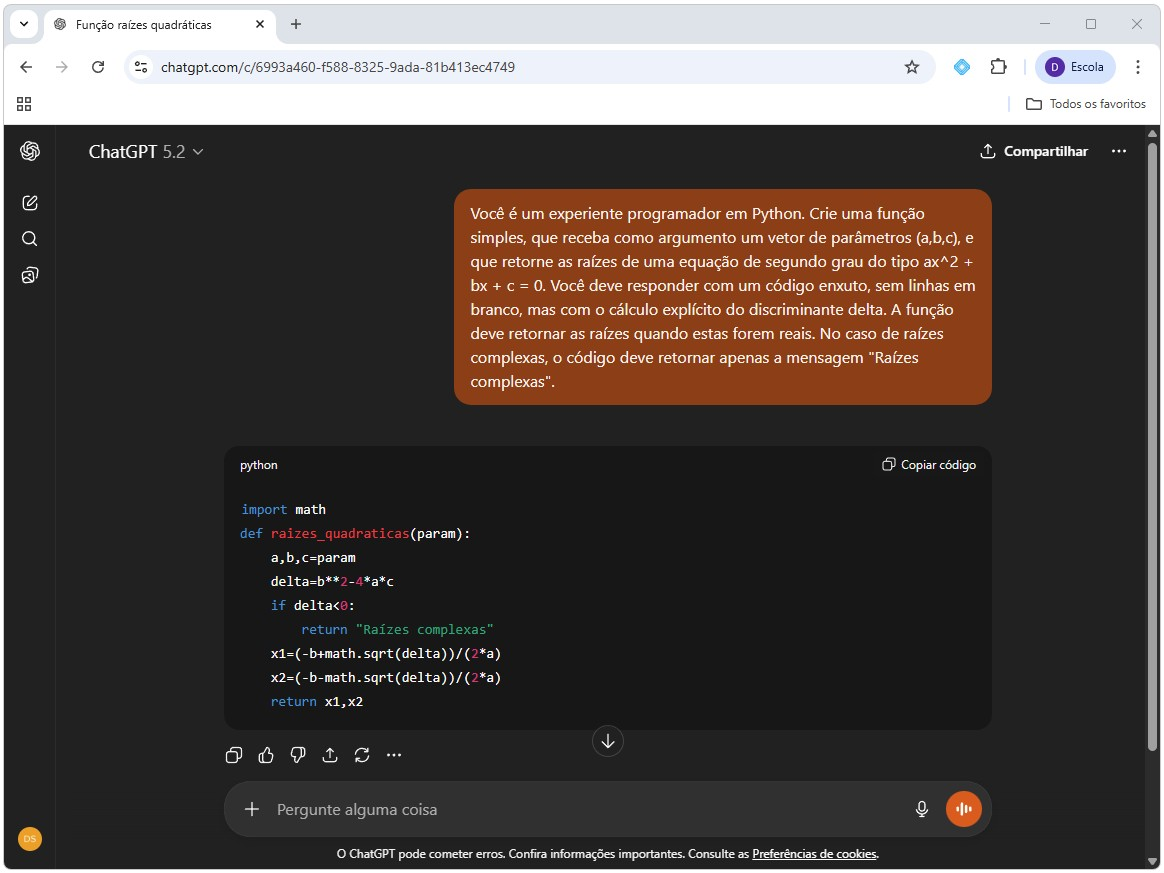
\includegraphics[width=8.33333in,height=\textheight,keepaspectratio]{images/chatgpt_bhaskara.jpg}

}

\caption{\label{fig-bhaskara}Exemplo de uso do ChatGPT em programação}

\end{figure}%

Um prompt ligeiramente diferente, com um grau menor de clareza e espaço
para ambiguidades, pode produzir resultados com a sintaxe correta mas
semanticamente errados, isto é, que ``rodem'' mas levem a uma conclusão
errada. No exemplo abaixo (Figura Figura~\ref{fig-bhaskara2}), o prompt
foi alterado de forma deliberada para pedir que a função ``retorne a
raiz'' ao invés de ``retorne as raízes''. Na maioria das vezes, a
ferramenta não vai apontar o erro matemático, produzindo como resposta
um código com a sintaxe correta mas que produza uma resposta
matematicamente incorreta. A Figura Figura~\ref{fig-bhaskara3} confronta
o ChatGPT, que explica a decisão em relação a resposta anterior.

\begin{figure}

\centering{

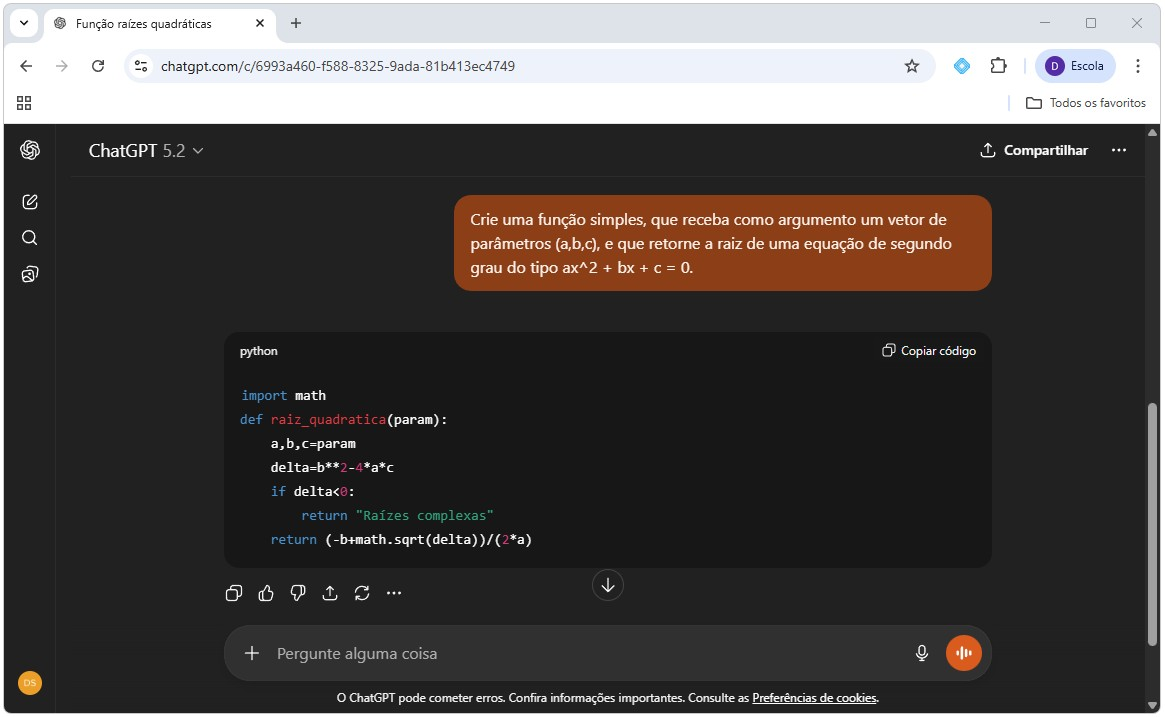
\includegraphics[width=8.33333in,height=\textheight,keepaspectratio]{images/chatgpt_bhaskara2.jpg}

}

\caption{\label{fig-bhaskara2}Exemplo de instrução incorreta}

\end{figure}%

\begin{figure}

\centering{

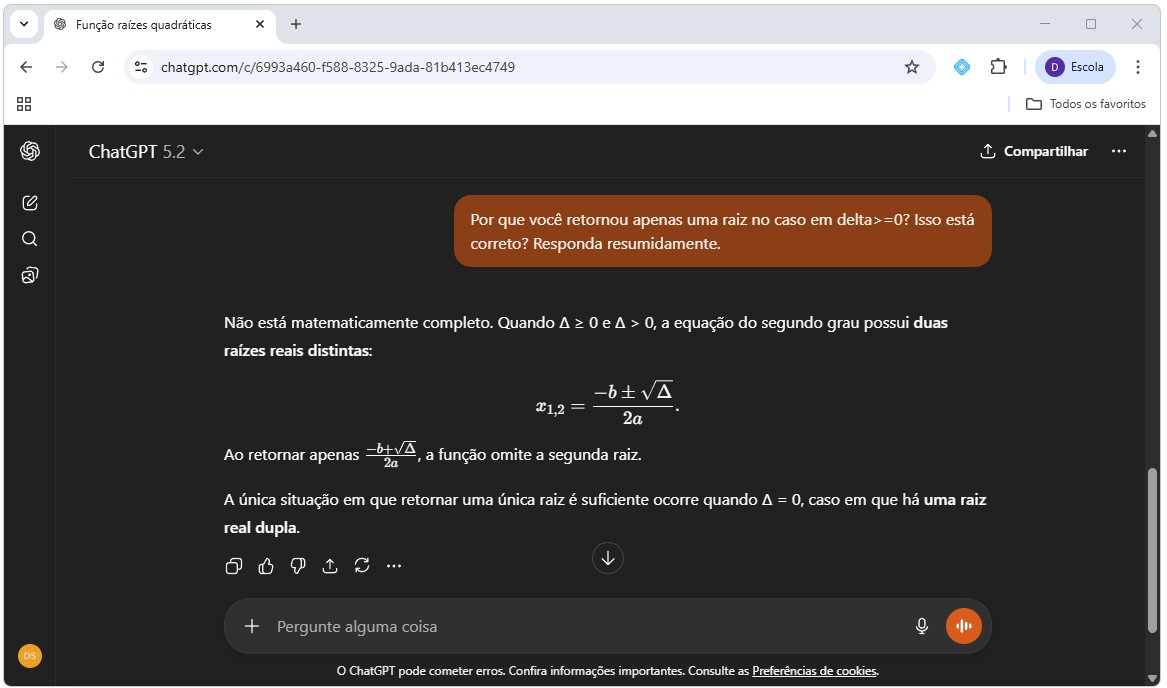
\includegraphics[width=8.33333in,height=\textheight,keepaspectratio]{images/chatgpt_bhaskara3.jpg}

}

\caption{\label{fig-bhaskara3}Justificativa do ChatGPT para a resposta
anterior}

\end{figure}%

\section{Riscos e limitações do uso de
IA}\label{riscos-e-limitauxe7uxf5es-do-uso-de-ia}

O principal risco do uso de IA no aprendizado de programação é a ilusão
de compreensão. Códigos gerados automaticamente podem funcionar, mas
isso não implica que o aluno compreenda sua lógica ou consiga
reproduzi-la em outra situação.

Outros riscos relevantes incluem:

\begin{itemize}
\tightlist
\item
  Geração de código incompatível com o problema e nível de conhecimento.
\item
  Soluções ineficientes ou computacionalmente custosas.
\item
  Erros semânticos, que não impedem o código de rodar, mas geram
  resultados incorretos em vista dos objetivos.
\end{itemize}

Por esses motivos, qualquer código sugerido por IA deve ser lido com
atenção, executado e testado, e comparado com o que foi visto em aula. A
regra prática é simples: se você não conseguir reconstruir ou adaptar a
solução sem a ferramenta de IA, então você não compreendeu a resposta
recebida e a ferramenta não deveria ter sido utilizada daquela forma ou
para aquele problema.

\section{Conclusão}\label{conclusuxe3o-2}

A IA representa uma mudança fundamental na forma como programamos, mas
não elimina a necessidade de compreender os fundamentos da computação.
Neste curso, a IA deve ser encarada como uma ferramenta auxiliar, útil
para esclarecer dúvidas, acelerar tarefas mecânicas e apoiar o processo
de aprendizagem, desde que usada de forma crítica e consciente.

O domínio de programação em Python exige prática, leitura de código,
compreensão de erros e construção gradual de raciocínio algorítmico.
Nenhuma ferramenta de IA substitui esse processo. Quando usada
corretamente, no entanto, ela pode torná-lo mais eficiente e menos
frustrante. Nos próximos capítulos, o foco retorna integralmente ao
desenvolvimento dessas habilidades fundamentais, que serão a base para
todas as aplicações computacionais em Economia ao longo do curso.

\section{Exercícios}\label{exercuxedcios-2}

\begin{enumerate}
\def\labelenumi{\arabic{enumi}.}
\item
  Considere um conjunto de dados hipotético contendo informações
  pessoais (nomes, datas de nascimento, renda). Explique em quais etapas
  e como você usaria ferramentas de IA generativa para auxiliar na
  análise desses dados. Quais são os principais riscos legais e éticos
  envolvidos?
\item
  Considere o código do exercício 4 do capítulo 3. Peça ao ChatGPT para
  explicar o(s) erro(s) contidos no script. Como você reescreveria o
  código, agora sem erros de sintaxe e/ou semântica?
\item
  Discorra sobre porque a atividade de programação é uma aplicação na
  qual o uso do ChatGPT é indicado e pode aumentar consideravelmente a
  produtividade.
\end{enumerate}

\chapter{Tipos primitivos e objetos básicos}\label{sec-objetos}

\section{Introdução}\label{introduuxe7uxe3o-3}

Este capítulo introduz os elementos fundamentais com os quais o Python
trabalha: valores, tipos e objetos. Em qualquer programa, manipulamos
dados -- números, textos, valores lógicos -- e precisamos compreender
como esses dados são representados, armazenados e transformados. Antes
de trabalhar com estruturas mais complexas, é necessário dominar os
tipos primitivos e entender que, em Python, tudo é um objeto. Todo
grande algoritmo e programa é construído a partir dos mesmos pequenos
blocos.

\begin{figure}

\centering{

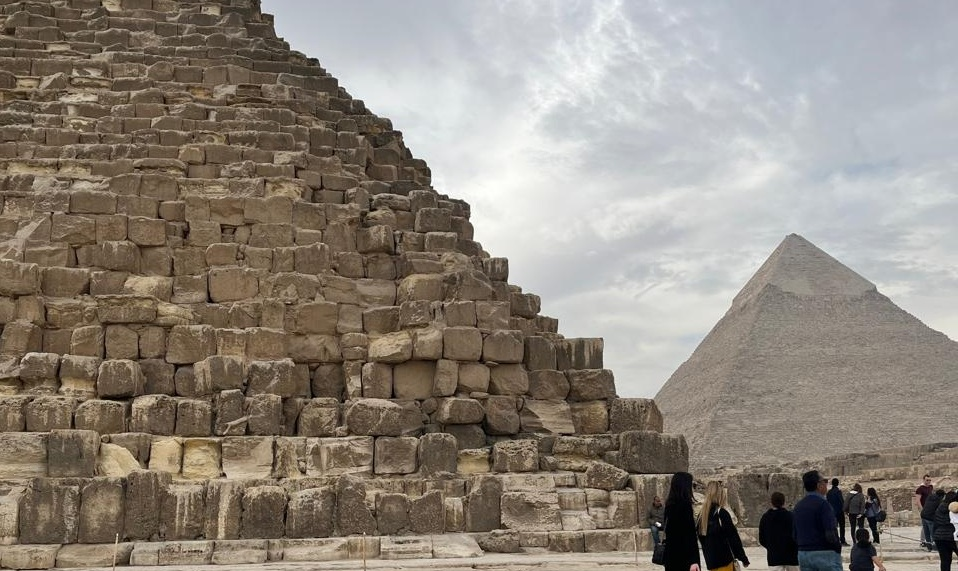
\includegraphics[width=8.33333in,height=\textheight,keepaspectratio]{images/piramides.jpeg}

}

\caption{\label{fig-olddesk}Blocos que formam a Pirâmide de Quéops e
Pirâmide de Quéfren ao fundo, 2024.}

\end{figure}%

Começaremos discutindo os tipos primitivos, que constituem a base de
toda manipulação de dados e determinam a forma como a informação é
armazenada, quais operações são permitidas e como o valor ocupa a
memória. Em seguida, generalizaremos para a noção de objeto e
discutiremos como propriedades e métodos estruturam o comportamento
desses valores.

\subsection{Pré-requisitos}\label{pruxe9-requisitos-3}

Nesse capítulo utilizaremos essencialmente funções nativas do Python. No
entanto, para trabalhar com padrões textuais de forma mais profunda,
utilizaremos alguns pacotes externos, em especial para lidar com as
chamadas \emph{expressões regulares}.

\begin{itemize}
\tightlist
\item
  \texttt{re}
\end{itemize}

\begin{Shaded}
\begin{Highlighting}[]
\ImportTok{import}\NormalTok{ re}
\end{Highlighting}
\end{Shaded}

\section{Tipos primitivos}\label{tipos-primitivos}

Antes de introduzirmos a noção geral de objeto, é fundamental
compreender os tipos mais elementares de dados disponíveis no Python, a
partir dos quais todas as estruturas mais complexas são construídas. Um
tipo de dado define a forma como a linguagem armazena e interpreta um
valor, isto é, um pedaço de informação que pode representar um número,
um texto ou um valor lógico. No caso de dados numéricos, há dois tipos
principais: \texttt{int}, utilizado para números inteiros, e
\texttt{float}, empregado para números com parte decimal. Informações
textuais são armazenadas no tipo \texttt{str} (abreviação de
\emph{string}). Por fim, valores lógicos pertencem ao tipo \texttt{bool}
e podem assumir apenas dois estados possíveis: \emph{True} ou
\emph{False}.

\begin{itemize}
\item
  \texttt{int}: representa números inteiros, que podem ser positivos,
  negativos ou zero. Como discutido no Capítulo~\ref{sec-fundamentos}, é
  fácil representar um número inteiro no sistema binário. Em um sistema
  de 8 bits, por exemplo, é possível representar valores entre 0 e 255
  no conjunto dos inteiros não negativos. O tamanho de um número
  inteiro, no entanto, não é fixo em 8 bits, ele pode crescer até 64
  bits conforme necessário e a memória disponível.
\item
  \texttt{float}: representa números com parte inteira e parte decimal.
  Esses valores são armazenados internamente em ponto flutuante binário,
  o que implica aproximação computacional na maioria dos casos e demanda
  um certo número de bits para representar a parte inteira e um outro
  númro de bits para representar o decimal. Isso ocorre tanto para
  números aparentemente simples, como \(2.5\) ou \(0.0390625\), quanto
  para dízimas periódicas, como \(0.333...\), ou números irracionais,
  como o \(\pi\). Como regra geral, quanto maior a precisão desejada,
  maior o custo em memória. Essa relação entre precisão, armazenamento e
  memória será retomada em um capítulo posterior.
\item
  \texttt{str}: utilizado para armazenar informações textuais, esse tipo
  representa sequências ordenadas de caracteres. Em outras palavras, a
  ordem importa: o string ``abc'' é diferente do string ``bca''. No
  Python, qualquer valor delimitado por aspas simples ou aspas duplas é
  considerado um string dentro da linguagem.
\item
  \texttt{bool}: armazena valores lógicos, que frequentemente são
  resultado de algum tipo de comparação. Valores booleanos serão
  essenciais quando estudarmos estruturas de controle, como instruções
  condicionais e métodos de iteração no próximo capítulo.
\end{itemize}

Compreender os tipos primitivos, suas propriedades e finalidades é
essencial para evitar erros comuns, como a tentativa de realizar
operações entre tipos incompatíveis. Além disso, o comportamento de um
operador depende diretamente do tipo dos valores envolvidos. Lembre-se,
o Python é uma linguagem de tipagem forte, o que significa que não
realiza conversões automáticas entre strings e números quando a operação
é ambígua. Assim, enquanto o operador \texttt{+} na expressão
\texttt{\textquotesingle{}5\textquotesingle{}\ +\ \textquotesingle{}5\textquotesingle{}}
funciona como um operador de concatenação de strings, no caso de
\texttt{5\ +\ 5} ele representa uma soma aritmética simples. Tome
bastante cuidado com isso.

A seguir, generalizaremos essa discussão ao introduzir a noção de
objeto, que permite compreender como o Python organiza internamente
todos esses valores.

\section{Objetos básicos}\label{objetos-buxe1sicos}

Em Python, \emph{tudo} é um objeto. Isso significa que qualquer valor --
seja um número, um texto ou um valor lógico -- possui uma estrutura
interna bem definida. De forma simplificada, um objeto é caracterizado
por três elementos: (i) um tipo, que determina sua categoria; (ii) um
valor, que corresponde à informação que ele representa; e (iii) um
conjunto de métodos, isto é, operações específicas que podem ser
aplicadas a ele.

\subsection{Strings}\label{strings}

As strings ilustram de forma clara essa noção. Diferentemente de números
inteiros ou de ponto flutuante, que representam quantidades numéricas,
uma string representa uma sequência ordenada de caracteres. A ordem dos
caracteres é relevante, e cada string é delimitada por aspas simples ou
duplas. Relembrando nosso primeiro ``programa'' da aula passada, podemos
atribuir a uma variável a string \emph{`Hello, World'} usando aspas:

\begin{Shaded}
\begin{Highlighting}[]
\CommentTok{\#\# Uso de aspas simples}
\NormalTok{str1 }\OperatorTok{=} \StringTok{\textquotesingle{}Hello, World\textquotesingle{}}

\BuiltInTok{print}\NormalTok{(str1)}
\BuiltInTok{print}\NormalTok{(}\BuiltInTok{type}\NormalTok{(str1))}
\end{Highlighting}
\end{Shaded}

\begin{verbatim}
Hello, World
<class 'str'>
\end{verbatim}

\begin{Shaded}
\begin{Highlighting}[]
\CommentTok{\#\# Uso de aspas duplas}
\NormalTok{str2 }\OperatorTok{=} \StringTok{"Hello, World"}

\BuiltInTok{print}\NormalTok{(str2)}
\BuiltInTok{print}\NormalTok{(}\BuiltInTok{type}\NormalTok{(str2))}
\end{Highlighting}
\end{Shaded}

\begin{verbatim}
Hello, World
<class 'str'>
\end{verbatim}

Podemos ainda utilizar uma sequência de três aspas duplas e escrever
strings que percorram várias linhas. Isso é bastante útil na
documentação de funções personalizadas, como veremos no
Capítulo~\ref{sec-funcoes}.

\begin{Shaded}
\begin{Highlighting}[]
\NormalTok{str3 }\OperatorTok{=} \StringTok{"""Das Utopias}

\StringTok{Se as coisas são inatingíveis...ora!}
\StringTok{Não é motivo para não querê{-}las...}
\StringTok{Que tristes os caminhos, se não fora}
\StringTok{A presença distante das estrelas!}
\StringTok{           }
\StringTok{Mario Quintana }
\StringTok{"""}

\BuiltInTok{print}\NormalTok{(str3)}
\BuiltInTok{print}\NormalTok{(}\BuiltInTok{type}\NormalTok{(str3))}
\end{Highlighting}
\end{Shaded}

\begin{verbatim}
Das Utopias

Se as coisas são inatingíveis...ora!
Não é motivo para não querê-las...
Que tristes os caminhos, se não fora
A presença distante das estrelas!

Mario Quintana 

<class 'str'>
\end{verbatim}

\subsubsection{Operações básicas}\label{operauxe7uxf5es-buxe1sicas}

Por ser uma sequência de caracteres e não um número, operações
aritméticas, em geral, não são permitidas, mas outras operações o são.
Uma dessas operações é chamada de \emph{slicing} ou fatiamento, que nos
permite acessar um caracter ou uma sequência de caracteres específicos
do string utilizando a posição -- também chamada de índice -- desse(s)
caractere(s). No caso do string \emph{`Hello, World'}, para acessar a
segunda letra podemos utilizar colchetes após o string e dentro dele o
índice referente à posição do `e' no string:

\begin{Shaded}
\begin{Highlighting}[]
\BuiltInTok{print}\NormalTok{(str1)}
\BuiltInTok{print}\NormalTok{(str1[}\DecValTok{2}\NormalTok{])}
\end{Highlighting}
\end{Shaded}

\begin{verbatim}
Hello, World
l
\end{verbatim}

Ué, mas porque que obtivemos como resposta o caractere `l', que é o 3º
na sequência, e não o `e', que é o 2º elemento? Aqui vai uma
particularidade da sintaxe do Python: em se tratando de índices, o
Python sempre começa a contagem em 0. Dessa forma, para acessar o
primeiro caractere de \emph{`Hello, World'} devemos pedir
\texttt{str1{[}0{]}}, para acessar o segundo é preciso pedir
\texttt{str1{[}1{]}} e assim por diante. Além disso, podemos acessar
contando de trás para frente e usando um índice negativo. Finalmente, é
possível que o índice seja substituído por uma expressão, que deve
sempre retornar como resultado um número inteiro.

\begin{Shaded}
\begin{Highlighting}[]
\CommentTok{\# Extração do segundo caractere do string pelo índice positivo}
\BuiltInTok{print}\NormalTok{(str1[}\DecValTok{1}\NormalTok{])}

\CommentTok{\# Extração do segundo caractere do string pelo índice negativo}
\BuiltInTok{print}\NormalTok{(str1[}\OperatorTok{{-}}\DecValTok{11}\NormalTok{])}

\CommentTok{\# Extração do segundo caractere do string através de uma expressão}
\NormalTok{n }\OperatorTok{=} \DecValTok{0}
\BuiltInTok{print}\NormalTok{(str1[n}\OperatorTok{+}\DecValTok{1}\NormalTok{])}
\end{Highlighting}
\end{Shaded}

\begin{verbatim}
e
e
e
\end{verbatim}

Para extrair não um único caractere, mas uma sequência (ou fatia) de
caracteres do string podemos utilizar um intervalo de índices, que
inclui o caractere representado pelo índice inicial mas exclui o
caractere representado pelo índice final. Para extrair a primeira
palavra do string \emph{`Hello, World'}, por exemplo, devemos utilizar o
intervalo que começa em 0 (posição do `H') e termina em 5 (posição da
vírgula).

\begin{Shaded}
\begin{Highlighting}[]
\BuiltInTok{print}\NormalTok{(str1[}\DecValTok{0}\NormalTok{:}\DecValTok{5}\NormalTok{])}
\end{Highlighting}
\end{Shaded}

\begin{verbatim}
Hello
\end{verbatim}

Para além do fatiamento, é possível utilizar o operador aritmético
\texttt{+} como uma forma de ``somar'' strings. Formalmente, o que essa
operação faz é concatenar os strings, transformando múltiplos strings em
um novo objeto do tipo \texttt{str} que replica a ordem do primeiro
string, seguido dos caracteres ordenados do segundo (e terceiro,
quarto,\ldots) string.

\begin{Shaded}
\begin{Highlighting}[]
\NormalTok{uniao\_str }\OperatorTok{=}\NormalTok{ str1 }\OperatorTok{+} \StringTok{\textquotesingle{} {-}{-}{-} \textquotesingle{}} \OperatorTok{+}\NormalTok{ str2}
\BuiltInTok{print}\NormalTok{(}\BuiltInTok{type}\NormalTok{(uniao\_str))}
\BuiltInTok{print}\NormalTok{(uniao\_str)}
\end{Highlighting}
\end{Shaded}

\begin{verbatim}
<class 'str'>
Hello, World --- Hello, World
\end{verbatim}

Note, porém, que strings são \emph{imutáveis}, de modo que caso queira
substituir um dos caracteres dentro de um string é preciso utilizar uma
função específica para isso ou criar um novo string derivado do 1º.
Apenas tentar substituir um dos caracteres de um string já definido não
é permitido.

\begin{Shaded}
\begin{Highlighting}[]
\CommentTok{\# Tentemos substituir o \textquotesingle{}e\textquotesingle{} do str1 por \textquotesingle{}a\textquotesingle{}}
\NormalTok{str1[}\DecValTok{1}\NormalTok{] }\OperatorTok{=} \StringTok{\textquotesingle{}a\textquotesingle{}}
\end{Highlighting}
\end{Shaded}

\begin{Highlighting}
\textcolor{black}{TypeError: 'str' object does not support item assignment}
\textcolor{black}{}\textcolor{QuartoInternalColor4}{---------------------------------------------------------------------------}\textcolor{QuartoInternalColor2}{}
\textcolor{QuartoInternalColor2}{}\textcolor{QuartoInternalColor4}{TypeError}\textcolor{QuartoInternalColor2}{                                 Traceback (most recent call last)}
\textcolor{QuartoInternalColor2}{}\textcolor{QuartoInternalColor1}{Cell}\textcolor{QuartoInternalColor2}{}\textcolor{QuartoInternalColor1}{ }\textcolor{QuartoInternalColor2}{}\textcolor{QuartoInternalColor3}{In[9]}\textcolor{QuartoInternalColor2}{}\textcolor{QuartoInternalColor3}{, line 2}\textcolor{QuartoInternalColor2}{}
\textcolor{QuartoInternalColor2}{}\textcolor{QuartoInternalColor3}{      1}\textcolor{QuartoInternalColor2}{ }\textcolor{QuartoInternalColor5}{# Tentemos substituir o 'e' do str1 por 'a'}\textcolor{QuartoInternalColor2}{}
\textcolor{QuartoInternalColor2}{}\textcolor{QuartoInternalColor3}{----> }\textcolor{QuartoInternalColor2}{}\textcolor{QuartoInternalColor3}{2}\textcolor{QuartoInternalColor2}{ }\textcolor{QuartoInternalColor2}{str1}\textcolor{QuartoInternalColor2}{}\textcolor{QuartoInternalColor2}{[}\textcolor{QuartoInternalColor2}{}\textcolor{QuartoInternalColor2}{1}\textcolor{QuartoInternalColor2}{}\textcolor{QuartoInternalColor2}{]}\textcolor{QuartoInternalColor2}{ = }\textcolor{QuartoInternalColor6}{'}\textcolor{QuartoInternalColor2}{}\textcolor{QuartoInternalColor6}{a}\textcolor{QuartoInternalColor2}{}\textcolor{QuartoInternalColor6}{'}\textcolor{QuartoInternalColor2}{}
\textcolor{QuartoInternalColor2}{}\textcolor{QuartoInternalColor4}{TypeError}\textcolor{QuartoInternalColor2}{: 'str' object does not support item assignment}
\end{Highlighting}

\subsubsection{Métodos de strings}\label{muxe9todos-de-strings}

As strings oferecem métodos que executam várias operações úteis. Um
método é em essência uma sequência de instruções encapsuladas dentro de
um único comando que recebe argumentos e devolve um valor. Embora a
sintaxe seja diferente, a ideia é a mesma quando falamos de funções,
objeto do nosso estudo daqui algumas aulas.

No caso dos métodos, temos que passar o nome da string que foi definida
anteriormente seguida de `.' e depois do comando relacionado ao método
específico. Considere um string de exemplo nomeado como
\texttt{str\_example}.

\begin{Shaded}
\begin{Highlighting}[]
\NormalTok{str\_example}\OperatorTok{=}\StringTok{\textquotesingle{} Hello, World\textquotesingle{}}
\end{Highlighting}
\end{Shaded}

Dentre os principais métodos aplicáveis a strings e suas funcionalidades
podemos citar:

\begin{enumerate}
\def\labelenumi{\arabic{enumi}.}
\tightlist
\item
  \textbf{str\_example.upper()} e \textbf{str\_example.lower()}: devolve
  a string \texttt{str\_example} toda em letras maiúsculas ou
  minúsculas, respectivamente.
\end{enumerate}

\begin{Shaded}
\begin{Highlighting}[]
\BuiltInTok{print}\NormalTok{(str\_example.upper())}
\BuiltInTok{print}\NormalTok{(str\_example.lower())}
\end{Highlighting}
\end{Shaded}

\begin{verbatim}
 HELLO, WORLD
 hello, world
\end{verbatim}

\begin{enumerate}
\def\labelenumi{\arabic{enumi}.}
\setcounter{enumi}{1}
\tightlist
\item
  \textbf{str\_example.strip()}: devolve a string retirando possíveis
  espaços em branco no início e no fim da string.
\end{enumerate}

\begin{Shaded}
\begin{Highlighting}[]
\BuiltInTok{print}\NormalTok{(str\_example.strip())}
\end{Highlighting}
\end{Shaded}

\begin{verbatim}
Hello, World
\end{verbatim}

\begin{enumerate}
\def\labelenumi{\arabic{enumi}.}
\setcounter{enumi}{2}
\tightlist
\item
  \textbf{str\_example.startswith(`xyz')} e
  \textbf{str\_example.endswith(`xyz')}: testa se a string começa ou
  termina, respectivamente, com os caracteres `xyz'.
\end{enumerate}

\begin{Shaded}
\begin{Highlighting}[]
\BuiltInTok{print}\NormalTok{(str\_example.startswith(}\StringTok{\textquotesingle{} \textquotesingle{}}\NormalTok{))}
\BuiltInTok{print}\NormalTok{(str\_example.endswith(}\StringTok{\textquotesingle{}d\textquotesingle{}}\NormalTok{))}
\end{Highlighting}
\end{Shaded}

\begin{verbatim}
True
True
\end{verbatim}

\begin{enumerate}
\def\labelenumi{\arabic{enumi}.}
\setcounter{enumi}{3}
\tightlist
\item
  \textbf{str\_example.find(`xyz')}: procura a string `xyz' dentro de
  \texttt{str\_example} e retorna o primeiro índice onde `xyz' começa ou
  retorna -1 se nada for encontrado.
\end{enumerate}

\begin{Shaded}
\begin{Highlighting}[]
\BuiltInTok{print}\NormalTok{(str\_example.find(}\StringTok{\textquotesingle{},\textquotesingle{}}\NormalTok{))}
\end{Highlighting}
\end{Shaded}

\begin{verbatim}
6
\end{verbatim}

\begin{enumerate}
\def\labelenumi{\arabic{enumi}.}
\setcounter{enumi}{4}
\tightlist
\item
  \textbf{str\_example.replace(`old',`new')}: retorna uma string nova
  onde todas as ocorrências de `old' encontradas serão substituídas por
  `new'.
\end{enumerate}

\begin{Shaded}
\begin{Highlighting}[]
\BuiltInTok{print}\NormalTok{(str\_example.replace(}\StringTok{\textquotesingle{}Hello\textquotesingle{}}\NormalTok{,}\StringTok{\textquotesingle{}World\textquotesingle{}}\NormalTok{))}
\end{Highlighting}
\end{Shaded}

\begin{verbatim}
 World, World
\end{verbatim}

Além desses principais, existem outros vários métodos para strings. Esse
\href{https://docs.python.org/pt-br/3/library/stdtypes.html\#textseq}{link}
é um bom ponto de partida para quem quiser conhecer outros exemplos.

\subsubsection{Formatação e a instrução
print}\label{formatauxe7uxe3o-e-a-instruuxe7uxe3o-print}

Um método sobre o qual não falamos, mas que é bastante interessante
quando queremos, por exemplo, printar o resultado de determinada
operação é \texttt{s.format()}. Com esse método podemos converter uma
variável numérica para uma formato específico e printá-la dentro de um
string maior. Imagine, por exemplo, que estejamos interessados em
printar o valor de \(\pi\) arredondado para 2 casas decimais apenas
dentro de um string que diz isso. Podemos implementar isso da seguinte
forma

\begin{Shaded}
\begin{Highlighting}[]
\NormalTok{pi }\OperatorTok{=} \FloatTok{3.1415926535}
\NormalTok{string\_base}\OperatorTok{=}\StringTok{\textquotesingle{}O valor de pi arredondado para 2 casas decimais é }\SpecialCharTok{\{:.2f\}}\StringTok{. Interessante, não?\textquotesingle{}}

\BuiltInTok{print}\NormalTok{(string\_base.}\BuiltInTok{format}\NormalTok{(pi))}
\end{Highlighting}
\end{Shaded}

\begin{verbatim}
O valor de pi arredondado para 2 casas decimais é 3.14. Interessante, não?
\end{verbatim}

Os colchetes dentro do string mostram onde que o número deve aparecer.
Mais do que isso, definimos dentro do colchete o formato do número. Após
os `:', o `.2' significa que queremos 2 casas decimais enquanto `f'
significa que queremos um formato de ponto fixo. Não vou entrar nos
detalhes de todas as formatações possíveis, mas podemos ver um pouco
mais disso
\href{https://www.w3schools.com/python/ref_string_format.asp}{aqui}.

\subsubsection{Introdução a expressões
regulares}\label{introduuxe7uxe3o-a-expressuxf5es-regulares}

Por vezes queremos encontrar um padrão específico de texto (e.g., placas
de carro, e-mails ou números de telefone) dentro de um texto maior, para
realizar algum tipo de coleta, limpeza ou mesmo substituição que um
simples \texttt{str.replace()} não dá conta. Para realizar tal ação
podemos utilizar as famosas \emph{Expressões Regulares}, também
conhecidas como \emph{Regular Expressions} no inglês, ou simplesmente
\emph{Regex}.

As expressões regulares são em essência uma potente linguagem para
especificar padrões de texto. De forma mais detalhada, é uma composição
dos chamados metacaracteres, caracteres com funções especiais, que,
agrupados entre si e em conjunto com caracteres literais, formam uma
sequência, uma expressão. Essa expressão é interpretada como uma regra
que indicará sucesso se uma entrada de dados qualquer casar com essa
regra, ou seja, obedecer exatamente a todas as suas condições.

Imagine que você tenha o string abaixo, que mostra o texto de um trecho
de uma notícia da CNN sobre o resultado da Pesquisa Datafolha para
presidente divulgada em 18/08/2022 (link para a matéria completa
\href{https://www.cnnbrasil.com.br/politica/pesquisa-datafolha-para-presidente-lula-tem-47-bolsonaro-32/}{aqui}).

\begin{Shaded}
\begin{Highlighting}[]
\NormalTok{pesquisa }\OperatorTok{=} \StringTok{"""}
\StringTok{Pesquisa Datafolha divulgada nesta quinta{-}feira (18) mostra o ex{-}presidente Luiz Inácio Lula da Silva (PT) à frente, }
\StringTok{com 47}\SpecialCharTok{\% d}\StringTok{as intenções de voto na corrida pelo Palácio do Planalto. O presidente Jair Bolsonaro (PL) tem 32\%. }
\StringTok{O primeiro turno das eleições acontece em 2 de outubro.}

\StringTok{Na sequência, aparecem Ciro Gomes (PDT), com 7\%; Simone Tebet (MDB), com 2\%, e Vera Lúcia (PSTU), com 1\%.}
\StringTok{"""}
\BuiltInTok{print}\NormalTok{(pesquisa)}
\end{Highlighting}
\end{Shaded}

\begin{verbatim}

Pesquisa Datafolha divulgada nesta quinta-feira (18) mostra o ex-presidente Luiz Inácio Lula da Silva (PT) à frente, 
com 47% das intenções de voto na corrida pelo Palácio do Planalto. O presidente Jair Bolsonaro (PL) tem 32%. 
O primeiro turno das eleições acontece em 2 de outubro.

Na sequência, aparecem Ciro Gomes (PDT), com 7%; Simone Tebet (MDB), com 2%, e Vera Lúcia (PSTU), com 1%.
\end{verbatim}

E se quiséssemos, por exemplo, substituir todas as porcentagens de
intenção de voto por `ZZZ'? Note que as porcentagens são diferentes e
não há uma repetição dos números que nos permita usar o
\texttt{str.replace()} de uma vez só. No entanto, todas as porcentagens
são representadas por 1 ou 2 números inteiros seguidos do símbolo
\(\%\). Nesse caso, o mais indicado é utilizar as expressões regulares.

Os módulos e funções nativas do Python não nos trazem muito material
para trabalhar com expressões regulares. Para operar com elas
utilizaremos uma biblioteca de comandos chamada \texttt{re}. Falaremos
mais sobre importação de bibliotecas de comandos e funções mais a
frente, mas por hora tenha na cabeça que para utilizar um conjunto de
instruções disponível em alguma biblioteca importada é preciso utilizar
o nome da biblioteca seguido de ponto e do nome da função dessa
biblioteca que você quer utilizar. No caso, para realizar a substituição
das porcentagens no string \emph{pesquisa} utilizaremos a função
\texttt{sub()} de dentro da biblioteca \texttt{re}. Mas o que devemos
colocar como input dessa função?

O mundo das expressões regulares é um mundo gigante e à parte, com
conteúdo suficiente para preencher um outro curso. De forma geral, a
combinação entre metacaracteres e caracteres literais é o que dá o
padrão do texto pelo qual procuramos. Alguns dos metacaracteres-padrão
são
\texttt{.\ ?\ *\ +\ \^{}\ \textbar{}\ {[}\ {]}\ \{\ \}\ (\ )\ \textbackslash{}},
cada um realizando uma função específica. Para o nosso caso utilizaremos
basicamente a expressão regular dada por

\texttt{{[}0-9{]}\{1,2\}\%}

Mas o que essa coisa bizarra diz de fato? A função buscará todo e
qualquer elemento dentro dos colchetes (no caso os dígitos numéricos)
que apareça uma ou duas vezes (código dentro dos colchetes) e que seja
seguido pelo símbolo de porcentagem. Note que esse é o padrão de
qualquer uma das porcentagens no nosso string \emph{pesquisa}. Vamos ver
o que acontece se usarmos isso dentro de \texttt{re.sub()}.

\begin{Shaded}
\begin{Highlighting}[]
\NormalTok{pesquisa2 }\OperatorTok{=}\NormalTok{ re.sub(}\StringTok{\textquotesingle{}[0{-}9]\{1,2\}\%\textquotesingle{}}\NormalTok{,}\StringTok{\textquotesingle{}ZZZ\textquotesingle{}}\NormalTok{,pesquisa)}

\BuiltInTok{print}\NormalTok{(pesquisa2)}
\end{Highlighting}
\end{Shaded}

\begin{verbatim}

Pesquisa Datafolha divulgada nesta quinta-feira (18) mostra o ex-presidente Luiz Inácio Lula da Silva (PT) à frente, 
com ZZZ das intenções de voto na corrida pelo Palácio do Planalto. O presidente Jair Bolsonaro (PL) tem ZZZ. 
O primeiro turno das eleições acontece em 2 de outubro.

Na sequência, aparecem Ciro Gomes (PDT), com ZZZ; Simone Tebet (MDB), com ZZZ, e Vera Lúcia (PSTU), com ZZZ.
\end{verbatim}

Conseguimos exatamente o que a gente queria. Boa, time!

Pare um pouco e pense sobre a aplicabilidade dessa ferramenta dentro de
um mundo repleto de dados não-estruturados, como tweets e notícias. O
potencial de uso é gigante! Mas como dissemos, o mundo de \emph{regex} é
muito grande e existem cursos e livros que se dedicam integralmente a
estudar essa linguagem de padrões textuais. Uma boa referência
introdutória é o livro
\href{https://www.amazon.com.br/Express\%C3\%B5es-Regulares-Uma-Abordagem-Divertida/dp/8575224743}{Expressões
Regulares: Uma Abordagem Divertida}.

\subsection{Listas}\label{listas}

Como uma string, uma lista é uma sequência de valores. Em uma string, os
valores são caracteres; em uma lista, eles podem ser de qualquer tipo.
Podemos ter uma lista de strings, uma lista de valores numéricos ou
mesmo uma lista de listas, combinando strings, números e mesmo outros
tipos de objetos que ainda veremos, como tuplas, dicionários e
dataframes.

Uma lista é delimitada por colchetes e os elementos, ou itens,
pertencentes a ela são separados por vírgula. Para definir uma lista com
5 números inteiros, ordenados de forma sequencial e começando em 1
devemos escrever a seguinte linha de código:

\begin{Shaded}
\begin{Highlighting}[]
\NormalTok{lista1 }\OperatorTok{=}\NormalTok{ [}\DecValTok{1}\NormalTok{,}\DecValTok{2}\NormalTok{,}\DecValTok{3}\NormalTok{,}\DecValTok{4}\NormalTok{,}\DecValTok{5}\NormalTok{]}

\BuiltInTok{print}\NormalTok{(}\BuiltInTok{type}\NormalTok{(lista1))}
\BuiltInTok{print}\NormalTok{(lista1)}
\end{Highlighting}
\end{Shaded}

\begin{verbatim}
<class 'list'>
[1, 2, 3, 4, 5]
\end{verbatim}

Podemos definir uma lista de strings, uma lista mista de strings e
números, e uma lista composto por outras listas (lista aninhada):

\begin{Shaded}
\begin{Highlighting}[]
\NormalTok{lista2 }\OperatorTok{=}\NormalTok{ [}\StringTok{\textquotesingle{}Danilo Souza\textquotesingle{}}\NormalTok{,}\StringTok{\textquotesingle{}Artur Viaro\textquotesingle{}}\NormalTok{]}
\NormalTok{lista3 }\OperatorTok{=}\NormalTok{ [}\StringTok{\textquotesingle{}Turma 2026101\textquotesingle{}}\NormalTok{,}\FloatTok{43.0}\NormalTok{,}\StringTok{\textquotesingle{}Turmas 2026102\textquotesingle{}}\NormalTok{,}\DecValTok{25}\NormalTok{,}\StringTok{\textquotesingle{}Turmas 2026121\textquotesingle{}}\NormalTok{,}\DecValTok{39}\NormalTok{,}\StringTok{\textquotesingle{}Turmas 2026122\textquotesingle{}}\NormalTok{,}\DecValTok{45}\NormalTok{]}
\NormalTok{lista4 }\OperatorTok{=}\NormalTok{ [lista1, lista2]}

\BuiltInTok{print}\NormalTok{(lista2)}
\BuiltInTok{print}\NormalTok{(lista3)}
\BuiltInTok{print}\NormalTok{(lista4)}
\end{Highlighting}
\end{Shaded}

\begin{verbatim}
['Danilo Souza', 'Artur Viaro']
['Turma 2026101', 43.0, 'Turmas 2026102', 25, 'Turmas 2026121', 39, 'Turmas 2026122', 45]
[[1, 2, 3, 4, 5], ['Danilo Souza', 'Artur Viaro']]
\end{verbatim}

De forma análoga à listas com elementos não vazios, é possível definir
uma lista vazia utilizando apenas os colchetes:

\begin{Shaded}
\begin{Highlighting}[]
\NormalTok{lista\_vazia }\OperatorTok{=}\NormalTok{ []}

\BuiltInTok{print}\NormalTok{(lista\_vazia)}
\end{Highlighting}
\end{Shaded}

\begin{verbatim}
[]
\end{verbatim}

\subsubsection{Operações básicas}\label{operauxe7uxf5es-buxe1sicas-1}

A sintaxe para acessar os elementos de uma lista é a mesma que para
acessar os caracteres de uma string. A expressão dentro dos colchetes
especifica o índice ou o intervalo de índices. Lembrando que o índice no
Python começa em ZERO e não em UM.

\begin{Shaded}
\begin{Highlighting}[]
\BuiltInTok{print}\NormalTok{(lista2[}\DecValTok{0}\NormalTok{])}
\BuiltInTok{print}\NormalTok{(lista2[}\DecValTok{1}\NormalTok{])}
\BuiltInTok{print}\NormalTok{(lista3[}\OperatorTok{{-}}\DecValTok{1}\NormalTok{])}
\BuiltInTok{print}\NormalTok{(lista3[}\DecValTok{0}\NormalTok{:}\DecValTok{2}\NormalTok{])}
\end{Highlighting}
\end{Shaded}

\begin{verbatim}
Danilo Souza
Artur Viaro
45
['Turma 2026101', 43.0]
\end{verbatim}

Diferente das strings, no entanto, listas são objetos mutáveis, isto é,
objetos que podem ser alterados internamente. Quando o operador de
colchete aparece do lado esquerdo de uma atribuição, ele identifica o
elemento da lista que será atribuído. No exemplo abaixo, O segundo
elemento da lista \texttt{numbers} (índice 1), que era 123 na atribuição
inicial, passa a ser 5 após a substituição do elemento na lista.

\begin{Shaded}
\begin{Highlighting}[]
\NormalTok{numbers }\OperatorTok{=}\NormalTok{ [}\DecValTok{42}\NormalTok{, }\DecValTok{123}\NormalTok{]}
\NormalTok{numbers[}\DecValTok{1}\NormalTok{] }\OperatorTok{=} \DecValTok{5}

\BuiltInTok{print}\NormalTok{(numbers)}
\end{Highlighting}
\end{Shaded}

\begin{verbatim}
[42, 5]
\end{verbatim}

Índices de listas funcionam da mesma forma que os índices de strings:

\begin{itemize}
\item
  Qualquer expressão de números inteiros pode ser usada como índice.
\item
  Caso você tente extrair ou sobrescrever um elemento que não existe,
  você receberá um erro do tipo \texttt{IndexError}.
\item
  Se um índice tiver um valor negativo, ele conta de trás para a frente,
  a partir do final da lista.
\end{itemize}

Assim como com strings, é possível calcular o número de elementos em uma
lista utilizando a função integrada \texttt{len()} e ``concatenar'' ou
``somar'' listas utilizando apenas o operador aritmético \texttt{+}.

\begin{Shaded}
\begin{Highlighting}[]
\NormalTok{produtos\_mercado }\OperatorTok{=}\NormalTok{ [}\StringTok{\textquotesingle{}alface\textquotesingle{}}\NormalTok{,}\StringTok{\textquotesingle{}tomate\textquotesingle{}}\NormalTok{,}\StringTok{\textquotesingle{}arroz\textquotesingle{}}\NormalTok{,}\StringTok{\textquotesingle{}ovos\textquotesingle{}}\NormalTok{,}\StringTok{\textquotesingle{}carne moída\textquotesingle{}}\NormalTok{,}\StringTok{\textquotesingle{}sabão líquido\textquotesingle{}}\NormalTok{]}

\BuiltInTok{print}\NormalTok{(}\BuiltInTok{len}\NormalTok{(produtos\_mercado))}
\end{Highlighting}
\end{Shaded}

\begin{verbatim}
6
\end{verbatim}

\begin{Shaded}
\begin{Highlighting}[]
\NormalTok{novos\_produtos }\OperatorTok{=}\NormalTok{ [}\StringTok{\textquotesingle{}papel higiênico\textquotesingle{}}\NormalTok{,}\StringTok{\textquotesingle{}pasta de dente\textquotesingle{}}\NormalTok{]}

\NormalTok{lista\_concatenada }\OperatorTok{=}\NormalTok{ produtos\_mercado }\OperatorTok{+}\NormalTok{ novos\_produtos}
\BuiltInTok{print}\NormalTok{(lista\_concatenada)}
\end{Highlighting}
\end{Shaded}

\begin{verbatim}
['alface', 'tomate', 'arroz', 'ovos', 'carne moída', 'sabão líquido', 'papel higiênico', 'pasta de dente']
\end{verbatim}

\subsubsection{Métodos de listas}\label{muxe9todos-de-listas}

As listas também possuem métodos bastante úteis, que nos facilitam a
vida em várias dimensões. Considere uma lista de exemplo nomeada como
\texttt{list\_example}.

\begin{Shaded}
\begin{Highlighting}[]
\NormalTok{list\_example}\OperatorTok{=}\NormalTok{[}\StringTok{\textquotesingle{}a\textquotesingle{}}\NormalTok{, }\StringTok{\textquotesingle{}c\textquotesingle{}}\NormalTok{, }\StringTok{\textquotesingle{}b\textquotesingle{}}\NormalTok{]}
\end{Highlighting}
\end{Shaded}

Dentre os principais métodos aplicáveis a listas e suas funcionalidades
podemos citar:

\begin{enumerate}
\def\labelenumi{\arabic{enumi}.}
\tightlist
\item
  \textbf{lista\_example.append()}: adiciona um novo elemento ao fim da
  lista ``lista\_example''.
\end{enumerate}

\begin{Shaded}
\begin{Highlighting}[]
\NormalTok{list\_example.append(}\StringTok{\textquotesingle{}g\textquotesingle{}}\NormalTok{)}

\BuiltInTok{print}\NormalTok{(list\_example)}
\end{Highlighting}
\end{Shaded}

\begin{verbatim}
['a', 'c', 'b', 'g']
\end{verbatim}

\begin{enumerate}
\def\labelenumi{\arabic{enumi}.}
\setcounter{enumi}{1}
\tightlist
\item
  \textbf{lista\_example.extend(lista2)}: toma a lista
  ``lista\_example'' como argumento e adiciona todos os elementos de
  lista2 como novos elementos da lista inicial.
\end{enumerate}

\begin{Shaded}
\begin{Highlighting}[]
\NormalTok{l2 }\OperatorTok{=}\NormalTok{ [}\StringTok{\textquotesingle{}e\textquotesingle{}}\NormalTok{,}\StringTok{\textquotesingle{}d\textquotesingle{}}\NormalTok{,}\StringTok{\textquotesingle{}f\textquotesingle{}}\NormalTok{]}
\NormalTok{list\_example.extend(l2)}

\BuiltInTok{print}\NormalTok{(list\_example)}
\end{Highlighting}
\end{Shaded}

\begin{verbatim}
['a', 'c', 'b', 'g', 'e', 'd', 'f']
\end{verbatim}

\begin{enumerate}
\def\labelenumi{\arabic{enumi}.}
\setcounter{enumi}{2}
\tightlist
\item
  \textbf{lista\_example.sort()}: classifica os elementos de
  ``lista\_example'' em ordem ascendente.
\end{enumerate}

\begin{Shaded}
\begin{Highlighting}[]
\NormalTok{list\_example.sort()}

\BuiltInTok{print}\NormalTok{(list\_example)}
\end{Highlighting}
\end{Shaded}

\begin{verbatim}
['a', 'b', 'c', 'd', 'e', 'f', 'g']
\end{verbatim}

\begin{enumerate}
\def\labelenumi{\arabic{enumi}.}
\setcounter{enumi}{3}
\tightlist
\item
  \textbf{lista\_example.remove(x)}: exclui o elemento igual a ``x'' de
  ``lista\_example''. É um método bastante útil quando queremos excluir
  um elemento específico, mas não sabemos sua posição dentro da lista.
\end{enumerate}

\begin{Shaded}
\begin{Highlighting}[]
\NormalTok{list\_example.remove(}\StringTok{\textquotesingle{}e\textquotesingle{}}\NormalTok{)}

\BuiltInTok{print}\NormalTok{(list\_example)}
\end{Highlighting}
\end{Shaded}

\begin{verbatim}
['a', 'b', 'c', 'd', 'f', 'g']
\end{verbatim}

Note que a maior parte dos métodos de listas alteram a lista original
mas não retornam nenhum valor. Dessa forma, atribuir a um objeto o
resultado da aplicação de um método em uma lista não é uma boa prática.
Se você escrever \texttt{ts\ =\ t.sort()}, por exemplo, ficará
desapontado com o resultado.

\begin{Shaded}
\begin{Highlighting}[]
\NormalTok{t }\OperatorTok{=}\NormalTok{ [}\StringTok{\textquotesingle{}d\textquotesingle{}}\NormalTok{, }\StringTok{\textquotesingle{}c\textquotesingle{}}\NormalTok{, }\StringTok{\textquotesingle{}e\textquotesingle{}}\NormalTok{, }\StringTok{\textquotesingle{}b\textquotesingle{}}\NormalTok{, }\StringTok{\textquotesingle{}a\textquotesingle{}}\NormalTok{]}
\NormalTok{ts }\OperatorTok{=}\NormalTok{ t.sort()}

\BuiltInTok{print}\NormalTok{(ts)}
\end{Highlighting}
\end{Shaded}

\begin{verbatim}
None
\end{verbatim}

Assim como já explicamos, uma lista é uma sequência de valores e uma
string é uma sequência de caracteres, mas uma lista de caracteres não é
a mesma coisa que uma string. Para converter uma string em uma lista de
caracteres, você pode usar o comando \texttt{list}:

\begin{Shaded}
\begin{Highlighting}[]
\NormalTok{s }\OperatorTok{=} \StringTok{\textquotesingle{}aula\textquotesingle{}}
\NormalTok{t }\OperatorTok{=} \BuiltInTok{list}\NormalTok{(s)}
\BuiltInTok{print}\NormalTok{(t)}
\end{Highlighting}
\end{Shaded}

\begin{verbatim}
['a', 'u', 'l', 'a']
\end{verbatim}

A função \texttt{list} quebra uma string em letras individuais. Se você
quiser quebrar uma string em palavras, você pode usar o método
\texttt{split()}. Esse método admite um argumento adicional, chamado
\emph{delimiter}, que especifica quais caracteres podem ser usados para
demonstrar os limites das palavras. Isso é muito útil, por exemplo,
quando queremos separar um texto em palavras e fazer a contagem de
palavras que mais se repetem. Qual caracter deveríamos passar como
argumento em \texttt{split()} nesse caso?

\begin{Shaded}
\begin{Highlighting}[]
\NormalTok{j }\OperatorTok{=} \StringTok{\textquotesingle{}a pressa é inimiga da perfeição\textquotesingle{}}
\NormalTok{s }\OperatorTok{=}\NormalTok{ j.split(}\StringTok{\textquotesingle{} \textquotesingle{}}\NormalTok{)}

\BuiltInTok{print}\NormalTok{(s)}
\end{Highlighting}
\end{Shaded}

\begin{verbatim}
['a', 'pressa', 'é', 'inimiga', 'da', 'perfeição']
\end{verbatim}

O método \texttt{join()} é o contrário de \texttt{split()}. Ele toma uma
lista de strings e concatena os elementos. \texttt{join()}, no entanto,
é um método de string, então é preciso invocá-lo no string delimitador
(por exemplo, '' - ``) e passar a lista de strings como parâmetro:

\begin{Shaded}
\begin{Highlighting}[]
\NormalTok{s }\OperatorTok{=}\NormalTok{ [}\StringTok{\textquotesingle{}a\textquotesingle{}}\NormalTok{,}\StringTok{\textquotesingle{}pressa\textquotesingle{}}\NormalTok{,}\StringTok{\textquotesingle{}é\textquotesingle{}}\NormalTok{,}\StringTok{\textquotesingle{}inimiga\textquotesingle{}}\NormalTok{,}\StringTok{\textquotesingle{}da\textquotesingle{}}\NormalTok{,}\StringTok{\textquotesingle{}perfeição\textquotesingle{}}\NormalTok{]}
\NormalTok{j }\OperatorTok{=} \StringTok{\textquotesingle{} \textquotesingle{}}\NormalTok{.join(s)}

\BuiltInTok{print}\NormalTok{(j)}
\end{Highlighting}
\end{Shaded}

\begin{verbatim}
a pressa é inimiga da perfeição
\end{verbatim}

Além desses principais, existem outros vários métodos para listas. Esse
\href{https://developers.google.com/edu/python/lists}{link} é um bom
ponto de partida para quem quiser conhecer outros exemplos.

\subsection{Tuplas}\label{tuplas}

Agora falaremos de mais um tipo de objeto básico do Python, a tupla. Uma
tupla é uma sequência de valores. Os valores podem ser de qualquer tipo
e são indexados por números inteiros, o que faz das tuplas objetos
bastante parecidos com as listas. A diferença crucial está no fato de
que as tuplas são \emph{imutáveis}, assim como os strings. Em resumo,
uma tupla é uma lista de valores separados por vírgulas e delimitado por
parênteses (lembre que listas são delimitadas por colchetes):

\begin{Shaded}
\begin{Highlighting}[]
\NormalTok{t }\OperatorTok{=}\NormalTok{ (}\StringTok{\textquotesingle{}a\textquotesingle{}}\NormalTok{,}\StringTok{\textquotesingle{}b\textquotesingle{}}\NormalTok{,}\StringTok{\textquotesingle{}c\textquotesingle{}}\NormalTok{,}\StringTok{\textquotesingle{}d\textquotesingle{}}\NormalTok{,}\StringTok{\textquotesingle{}e\textquotesingle{}}\NormalTok{)}

\BuiltInTok{print}\NormalTok{(}\BuiltInTok{type}\NormalTok{(t))}
\end{Highlighting}
\end{Shaded}

\begin{verbatim}
<class 'tuple'>
\end{verbatim}

Note que um único valor entre parênteses não é uma tupla. Para criar uma
tupla com um único elemento, é preciso incluir uma vírgula final após o
elemento, com ou sem os parênteses.

\begin{Shaded}
\begin{Highlighting}[]
\NormalTok{t1 }\OperatorTok{=}\NormalTok{ (}\StringTok{\textquotesingle{}a\textquotesingle{}}\NormalTok{)}
\NormalTok{t2 }\OperatorTok{=} \StringTok{\textquotesingle{}a\textquotesingle{}}\NormalTok{,}
\NormalTok{t3 }\OperatorTok{=}\NormalTok{ (}\StringTok{\textquotesingle{}a\textquotesingle{}}\NormalTok{,)}

\BuiltInTok{print}\NormalTok{(}\BuiltInTok{type}\NormalTok{(t1))}
\BuiltInTok{print}\NormalTok{(}\BuiltInTok{type}\NormalTok{(t2))}
\BuiltInTok{print}\NormalTok{(}\BuiltInTok{type}\NormalTok{(t3))}
\end{Highlighting}
\end{Shaded}

\begin{verbatim}
<class 'str'>
<class 'tuple'>
<class 'tuple'>
\end{verbatim}

Outra forma de criar uma tupla é com a função integrada \texttt{tuple}.
Sem argumentos, cria uma tupla vazia. Se os argumentos forem uma
sequência (string, lista ou tupla), o resultado é uma tupla com os
elementos da sequência:

\begin{Shaded}
\begin{Highlighting}[]
\NormalTok{t1 }\OperatorTok{=} \BuiltInTok{tuple}\NormalTok{()}
\NormalTok{t2 }\OperatorTok{=} \BuiltInTok{tuple}\NormalTok{(}\StringTok{\textquotesingle{}tupla\textquotesingle{}}\NormalTok{)}

\BuiltInTok{print}\NormalTok{(t1)}
\BuiltInTok{print}\NormalTok{(t2)}
\end{Highlighting}
\end{Shaded}

\begin{verbatim}
()
('t', 'u', 'p', 'l', 'a')
\end{verbatim}

\subsubsection{Operações básicas}\label{operauxe7uxf5es-buxe1sicas-2}

A maior parte dos operadores de lista também funciona em tuplas. O uso
de colchetes após o nome da tupla serve para operações de indexação e
fatiamento, selecionando um único elemento ou uma sequência de vários
elementos.

\begin{Shaded}
\begin{Highlighting}[]
\NormalTok{t }\OperatorTok{=}\NormalTok{ (}\StringTok{\textquotesingle{}a\textquotesingle{}}\NormalTok{, }\StringTok{\textquotesingle{}b\textquotesingle{}}\NormalTok{, }\StringTok{\textquotesingle{}c\textquotesingle{}}\NormalTok{, }\StringTok{\textquotesingle{}d\textquotesingle{}}\NormalTok{, }\StringTok{\textquotesingle{}e\textquotesingle{}}\NormalTok{)}

\BuiltInTok{print}\NormalTok{(t[}\DecValTok{0}\NormalTok{])}
\BuiltInTok{print}\NormalTok{(t[}\DecValTok{1}\NormalTok{:}\DecValTok{3}\NormalTok{])}
\end{Highlighting}
\end{Shaded}

\begin{verbatim}
a
('b', 'c')
\end{verbatim}

Entretanto, se você tentar alterar um dos elementos da tupla, vai
receber um erro. Como tuplas são objetos imutáveis, você não pode
alterar seus elementos diretamente. Para ``alterar'' uma tupla, é
preciso criar uma nova tupla.

\begin{Shaded}
\begin{Highlighting}[]
\NormalTok{t[}\DecValTok{0}\NormalTok{] }\OperatorTok{=} \StringTok{\textquotesingle{}A\textquotesingle{}}
\end{Highlighting}
\end{Shaded}

\begin{Highlighting}
\textcolor{black}{TypeError: 'tuple' object does not support item assignment}
\textcolor{black}{}\textcolor{QuartoInternalColor4}{---------------------------------------------------------------------------}\textcolor{QuartoInternalColor2}{}
\textcolor{QuartoInternalColor2}{}\textcolor{QuartoInternalColor4}{TypeError}\textcolor{QuartoInternalColor2}{                                 Traceback (most recent call last)}
\textcolor{QuartoInternalColor2}{}\textcolor{QuartoInternalColor1}{Cell}\textcolor{QuartoInternalColor2}{}\textcolor{QuartoInternalColor1}{ }\textcolor{QuartoInternalColor2}{}\textcolor{QuartoInternalColor3}{In[39]}\textcolor{QuartoInternalColor2}{}\textcolor{QuartoInternalColor3}{, line 1}\textcolor{QuartoInternalColor2}{}
\textcolor{QuartoInternalColor2}{}\textcolor{QuartoInternalColor3}{----> }\textcolor{QuartoInternalColor2}{}\textcolor{QuartoInternalColor3}{1}\textcolor{QuartoInternalColor2}{ }\textcolor{QuartoInternalColor2}{t}\textcolor{QuartoInternalColor2}{}\textcolor{QuartoInternalColor2}{[}\textcolor{QuartoInternalColor2}{}\textcolor{QuartoInternalColor2}{0}\textcolor{QuartoInternalColor2}{}\textcolor{QuartoInternalColor2}{]}\textcolor{QuartoInternalColor2}{ = }\textcolor{QuartoInternalColor6}{'}\textcolor{QuartoInternalColor2}{}\textcolor{QuartoInternalColor6}{A}\textcolor{QuartoInternalColor2}{}\textcolor{QuartoInternalColor6}{'}\textcolor{QuartoInternalColor2}{}
\textcolor{QuartoInternalColor2}{}\textcolor{QuartoInternalColor4}{TypeError}\textcolor{QuartoInternalColor2}{: 'tuple' object does not support item assignment}
\end{Highlighting}

\subsubsection{Atribuição de tuplas}\label{atribuiuxe7uxe3o-de-tuplas}

Muitas vezes, é útil trocar os valores de duas variáveis. Com a
atribuição convencional, é preciso usar uma variável temporária. Essa
solução é trabalhosa; a atribuição de tuplas é mais elegante. Por
exemplo, trocar a e b.

\begin{Shaded}
\begin{Highlighting}[]
\NormalTok{a}\OperatorTok{=}\DecValTok{5}
\NormalTok{b}\OperatorTok{=}\DecValTok{6}

\NormalTok{temp }\OperatorTok{=}\NormalTok{ a}
\NormalTok{a }\OperatorTok{=}\NormalTok{ b}
\NormalTok{b }\OperatorTok{=}\NormalTok{ temp}

\BuiltInTok{print}\NormalTok{(b)}
\end{Highlighting}
\end{Shaded}

\begin{verbatim}
5
\end{verbatim}

Essa solução é trabalhosa; a atribuição de tuplas é mais elegante:

\begin{Shaded}
\begin{Highlighting}[]
\NormalTok{a}\OperatorTok{=}\DecValTok{5}
\NormalTok{b}\OperatorTok{=}\DecValTok{6}

\NormalTok{a, b }\OperatorTok{=}\NormalTok{ b, a}

\BuiltInTok{print}\NormalTok{(b)}
\end{Highlighting}
\end{Shaded}

\begin{verbatim}
5
\end{verbatim}

O lado esquerdo é uma tupla de variáveis e o lado direito é uma tupla de
expressões. Cada valor é atribuído à sua respectiva variável. De forma
geral, o lado direito pode ter qualquer tipo de sequência (string, lista
ou tupla). Por exemplo, para dividir um endereço de email em um nome de
usuário e um domínio, você poderia escrever utilizar o método
\texttt{split}. O valor de retorno do \texttt{split()} é uma lista com
dois elementos; o primeiro elemento é atribuído a \texttt{uname}, o
segundo a \texttt{domain}.

\begin{Shaded}
\begin{Highlighting}[]
\NormalTok{addr }\OperatorTok{=} \StringTok{\textquotesingle{}monty@python.org\textquotesingle{}}
\NormalTok{uname, domain }\OperatorTok{=}\NormalTok{ addr.split(}\StringTok{\textquotesingle{}@\textquotesingle{}}\NormalTok{)}

\BuiltInTok{print}\NormalTok{(uname)}
\BuiltInTok{print}\NormalTok{(domain)}
\end{Highlighting}
\end{Shaded}

\begin{verbatim}
monty
python.org
\end{verbatim}

\subsubsection{Operações nativas com
tuplas}\label{operauxe7uxf5es-nativas-com-tuplas}

A função nativa \texttt{zip} recebe duas ou mais sequências e devolve
uma lista de tuplas onde cada tupla contém um elemento de cada
sequência. O nome da função tem a ver com o zíper, que se junta e
encaixa duas carreiras de dentes. O resultado é um objeto \texttt{zip}
que sabe como percorrer os elementos pareados. O exemplo abaixo encaixa
uma string e uma lista:

\begin{Shaded}
\begin{Highlighting}[]
\NormalTok{s }\OperatorTok{=} \StringTok{\textquotesingle{}abc\textquotesingle{}}
\NormalTok{t }\OperatorTok{=}\NormalTok{ [}\DecValTok{0}\NormalTok{, }\DecValTok{1}\NormalTok{, }\DecValTok{2}\NormalTok{]}
\NormalTok{z }\OperatorTok{=} \BuiltInTok{zip}\NormalTok{(s,t)}

\BuiltInTok{print}\NormalTok{(z)}
\end{Highlighting}
\end{Shaded}

\begin{verbatim}
<zip object at 0x0000027A0DFA2280>
\end{verbatim}

Um objeto \texttt{zip} é um tipo de iterador, ou seja, qualquer objeto
que percorre ou itera sobre uma sequência. Iteradores são semelhantes a
listas em alguns aspectos, mas, ao contrário de listas, não é possível
usar um índice para selecionar um elemento de um iterador. Se quiser
usar operadores e métodos de lista, você pode usar um objeto
\texttt{zip} para fazer uma lista. O resultado é uma lista de tuplas.
Neste exemplo, cada tupla contém um caractere da string e o elemento
correspondente da lista.

\begin{Shaded}
\begin{Highlighting}[]
\BuiltInTok{print}\NormalTok{(}\BuiltInTok{list}\NormalTok{(z))}
\end{Highlighting}
\end{Shaded}

\begin{verbatim}
[('a', 0), ('b', 1), ('c', 2)]
\end{verbatim}

\subsection{Dicionários}\label{dicionuxe1rios}

Dicionários são um outro tipo de objeto bastante importante e útil em
nossas aplicações. Dicionários são um dos melhores recursos do Python,
eles são os blocos de montar de muitos algoritmos eficientes e
elegantes.

Um dicionário se parece com uma lista, mas é mais geral. Em uma lista,
os índices devem ser números inteiros, em um dicionário eles podem ser
de (quase) qualquer tipo. Um dicionário contém uma coleção de índices,
que se chamam chaves, e uma coleção de valores. \emph{Cada chave é
associada com um único valor}. A associação de uma chave e um valor
chama-se par chave-valor ou item.

Em linguagem matemática, um dicionário representa um mapeamento de
chaves a valores, para que você possa dizer que cada chave ``mostra o
mapa'' a um valor. Como exemplo, vamos construir um dicionário que faz o
mapa de palavras do inglês ao espanhol, de forma que tanto as chaves
quanto os valores sejam strings. A função \texttt{dict} cria um novo
dicionário sem itens. Como \texttt{dict} é o nome de uma função
integrada, você deve evitar usá-lo como nome de variável.

\begin{Shaded}
\begin{Highlighting}[]
\NormalTok{eng2sp }\OperatorTok{=} \BuiltInTok{dict}\NormalTok{()}

\NormalTok{eng2sp}
\end{Highlighting}
\end{Shaded}

\begin{verbatim}
{}
\end{verbatim}

As chaves \{\} representam um dicionário vazio. Para acrescentar itens
ao dicionário, você pode usar colchetes.

\begin{Shaded}
\begin{Highlighting}[]
\NormalTok{eng2sp[}\StringTok{\textquotesingle{}one\textquotesingle{}}\NormalTok{] }\OperatorTok{=} \StringTok{\textquotesingle{}uno\textquotesingle{}}
\end{Highlighting}
\end{Shaded}

Esta linha cria um item que mapeia da chave `one' ao valor `uno'. Se
imprimirmos o dicionário novamente, vemos um par chave-valor com dois
pontos entre a chave e o valor:

\begin{Shaded}
\begin{Highlighting}[]
\NormalTok{eng2sp}
\end{Highlighting}
\end{Shaded}

\begin{verbatim}
{'one': 'uno'}
\end{verbatim}

Este formato de saída também é um formato de entrada. Por exemplo, você
pode criar um dicionário com três itens:

\begin{Shaded}
\begin{Highlighting}[]
\NormalTok{eng2sp }\OperatorTok{=}\NormalTok{ \{}\StringTok{\textquotesingle{}one\textquotesingle{}}\NormalTok{: }\StringTok{\textquotesingle{}uno\textquotesingle{}}\NormalTok{, }\StringTok{\textquotesingle{}three\textquotesingle{}}\NormalTok{: }\StringTok{\textquotesingle{}tres\textquotesingle{}}\NormalTok{, }\StringTok{\textquotesingle{}two\textquotesingle{}}\NormalTok{: }\StringTok{\textquotesingle{}dos\textquotesingle{}}\NormalTok{, }\StringTok{\textquotesingle{}eleven\textquotesingle{}}\NormalTok{: }\StringTok{\textquotesingle{}once\textquotesingle{}}\NormalTok{\}}
\NormalTok{eng2sp}
\end{Highlighting}
\end{Shaded}

\begin{verbatim}
{'one': 'uno', 'three': 'tres', 'two': 'dos', 'eleven': 'once'}
\end{verbatim}

Ué, mas a ordem parece diferente daquela que definimos, não? Se você
digitar o mesmo exemplo no seu computador, pode receber um resultado
diferente. Em geral, a ordem dos itens em um dicionário é imprevisível.
No entanto, isso não é um problema porque os elementos de um dicionário
nunca são indexados com índices de números inteiros. Em vez disso, você
usa as chaves para procurar os valores correspondentes. A chave
\texttt{\textquotesingle{}two\textquotesingle{}}, por exemplo sempre
mapeia ao valor \texttt{\textquotesingle{}dos\textquotesingle{}}, assim
a ordem dos itens não importa.

\begin{Shaded}
\begin{Highlighting}[]
\NormalTok{eng2sp[}\StringTok{\textquotesingle{}two\textquotesingle{}}\NormalTok{]}
\end{Highlighting}
\end{Shaded}

\begin{verbatim}
'dos'
\end{verbatim}

Se a chave não estiver no dicionário, você recebe uma exceção:

\begin{Shaded}
\begin{Highlighting}[]
\NormalTok{eng2sp[}\StringTok{\textquotesingle{}four\textquotesingle{}}\NormalTok{]}
\end{Highlighting}
\end{Shaded}

\begin{Highlighting}
\textcolor{black}{KeyError: 'four'}
\textcolor{black}{}\textcolor{QuartoInternalColor4}{---------------------------------------------------------------------------}\textcolor{QuartoInternalColor2}{}
\textcolor{QuartoInternalColor2}{}\textcolor{QuartoInternalColor4}{KeyError}\textcolor{QuartoInternalColor2}{                                  Traceback (most recent call last)}
\textcolor{QuartoInternalColor2}{}\textcolor{QuartoInternalColor1}{Cell}\textcolor{QuartoInternalColor2}{}\textcolor{QuartoInternalColor1}{ }\textcolor{QuartoInternalColor2}{}\textcolor{QuartoInternalColor3}{In[50]}\textcolor{QuartoInternalColor2}{}\textcolor{QuartoInternalColor3}{, line 1}\textcolor{QuartoInternalColor2}{}
\textcolor{QuartoInternalColor2}{}\textcolor{QuartoInternalColor3}{----> }\textcolor{QuartoInternalColor2}{}\textcolor{QuartoInternalColor3}{1}\textcolor{QuartoInternalColor2}{ }\textcolor{QuartoInternalColor2}{eng2sp}\textcolor{QuartoInternalColor2}{}\textcolor{QuartoInternalColor2}{[}\textcolor{QuartoInternalColor2}{}\textcolor{QuartoInternalColor2}{'}\textcolor{QuartoInternalColor2}{}\textcolor{QuartoInternalColor2}{four}\textcolor{QuartoInternalColor2}{}\textcolor{QuartoInternalColor2}{'}\textcolor{QuartoInternalColor2}{}\textcolor{QuartoInternalColor2}{]}\textcolor{QuartoInternalColor2}{}
\textcolor{QuartoInternalColor2}{}\textcolor{QuartoInternalColor4}{KeyError}\textcolor{QuartoInternalColor2}{: 'four'}
\end{Highlighting}

\subsubsection{Operações básicas}\label{operauxe7uxf5es-buxe1sicas-3}

Podemos adicionar um novo par de chave e valor ao dicionário usando
colchetes. Caso a chave já exista no dicionário, é possível atualizar o
valor.

\begin{Shaded}
\begin{Highlighting}[]
\NormalTok{y }\OperatorTok{=}\NormalTok{ \{\}}
\NormalTok{y[}\StringTok{\textquotesingle{}one\textquotesingle{}}\NormalTok{] }\OperatorTok{=} \DecValTok{1}
\NormalTok{y[}\StringTok{\textquotesingle{}two\textquotesingle{}}\NormalTok{] }\OperatorTok{=} \DecValTok{2}

\BuiltInTok{print}\NormalTok{(y)}
\end{Highlighting}
\end{Shaded}

\begin{verbatim}
{'one': 1, 'two': 2}
\end{verbatim}

\begin{Shaded}
\begin{Highlighting}[]
\NormalTok{y[}\StringTok{\textquotesingle{}two\textquotesingle{}}\NormalTok{] }\OperatorTok{=} \StringTok{\textquotesingle{}dos\textquotesingle{}}
\BuiltInTok{print}\NormalTok{(y)}
\end{Highlighting}
\end{Shaded}

\begin{verbatim}
{'one': 1, 'two': 'dos'}
\end{verbatim}

A instrução \texttt{del} pode ser usada para remover uma entrada (par de
valor de chave) de um dicionário.

\begin{Shaded}
\begin{Highlighting}[]
\KeywordTok{del}\NormalTok{ y[}\StringTok{\textquotesingle{}two\textquotesingle{}}\NormalTok{]}
\BuiltInTok{print}\NormalTok{(y)}
\end{Highlighting}
\end{Shaded}

\begin{verbatim}
{'one': 1}
\end{verbatim}

Tente acessar uma chave que não está em um dicionário e você receberá um
erro de exceção do Python. Para lidar com essa exceção, você pode usar o
operador \texttt{in} que testa se existe uma chave em um dicionário.
Esse operador retorna \emph{True} se o dicionário tiver um valor
armazenado sob a chave fornecida e \emph{False} caso contrário.

\begin{Shaded}
\begin{Highlighting}[]
\KeywordTok{del}\NormalTok{ y[}\StringTok{\textquotesingle{}three\textquotesingle{}}\NormalTok{]}
\end{Highlighting}
\end{Shaded}

\begin{Highlighting}
\textcolor{black}{KeyError: 'three'}
\textcolor{black}{}\textcolor{QuartoInternalColor4}{---------------------------------------------------------------------------}\textcolor{QuartoInternalColor2}{}
\textcolor{QuartoInternalColor2}{}\textcolor{QuartoInternalColor4}{KeyError}\textcolor{QuartoInternalColor2}{                                  Traceback (most recent call last)}
\textcolor{QuartoInternalColor2}{}\textcolor{QuartoInternalColor1}{Cell}\textcolor{QuartoInternalColor2}{}\textcolor{QuartoInternalColor1}{ }\textcolor{QuartoInternalColor2}{}\textcolor{QuartoInternalColor3}{In[54]}\textcolor{QuartoInternalColor2}{}\textcolor{QuartoInternalColor3}{, line 1}\textcolor{QuartoInternalColor2}{}
\textcolor{QuartoInternalColor2}{}\textcolor{QuartoInternalColor3}{----> }\textcolor{QuartoInternalColor2}{}\textcolor{QuartoInternalColor3}{1}\textcolor{QuartoInternalColor2}{ }\textcolor{QuartoInternalColor7}{del}\textcolor{QuartoInternalColor2}{ }\textcolor{QuartoInternalColor2}{y}\textcolor{QuartoInternalColor2}{}\textcolor{QuartoInternalColor2}{[}\textcolor{QuartoInternalColor2}{}\textcolor{QuartoInternalColor2}{'}\textcolor{QuartoInternalColor2}{}\textcolor{QuartoInternalColor2}{three}\textcolor{QuartoInternalColor2}{}\textcolor{QuartoInternalColor2}{'}\textcolor{QuartoInternalColor2}{}\textcolor{QuartoInternalColor2}{]}\textcolor{QuartoInternalColor2}{}
\textcolor{QuartoInternalColor2}{}\textcolor{QuartoInternalColor4}{KeyError}\textcolor{QuartoInternalColor2}{: 'three'}
\end{Highlighting}

\begin{Shaded}
\begin{Highlighting}[]
\CommentTok{\textquotesingle{}three\textquotesingle{}} \KeywordTok{in}\NormalTok{ y}
\end{Highlighting}
\end{Shaded}

\begin{verbatim}
False
\end{verbatim}

\subsubsection{Métodos de
dicionários}\label{muxe9todos-de-dicionuxe1rios}

Considere o dicionário de exemplo abaixo.

\begin{Shaded}
\begin{Highlighting}[]
\NormalTok{dict\_example }\OperatorTok{=}\NormalTok{ \{}\StringTok{\textquotesingle{}one\textquotesingle{}}\NormalTok{:}\DecValTok{1}\NormalTok{,}\StringTok{\textquotesingle{}two\textquotesingle{}}\NormalTok{:}\DecValTok{2}\NormalTok{,}\StringTok{\textquotesingle{}three\textquotesingle{}}\NormalTok{:}\DecValTok{3}\NormalTok{,}\StringTok{\textquotesingle{}four\textquotesingle{}}\NormalTok{:}\DecValTok{4}\NormalTok{\}}
\end{Highlighting}
\end{Shaded}

Dentre os principais métodos aplicáveis a dicionários e suas
funcionalidades podemos citar:

\begin{enumerate}
\def\labelenumi{\arabic{enumi}.}
\tightlist
\item
  \textbf{dict\_example.update(x)}: atualiza o dicionário
  \texttt{dict\_example} com todos os pares de valor-chave de um segundo
  dicionário \texttt{dict\_update}. Os valores de chaves, que são comuns
  a ambos os dicionários, do segundo dicionário irão se sobrepor aos
  valores das chaves do primeiro dicionário.
\end{enumerate}

\begin{Shaded}
\begin{Highlighting}[]
\NormalTok{dict\_update }\OperatorTok{=}\NormalTok{ \{}\StringTok{\textquotesingle{}four\textquotesingle{}}\NormalTok{:}\DecValTok{4}\NormalTok{,}\StringTok{\textquotesingle{}five\textquotesingle{}}\NormalTok{:}\DecValTok{5}\NormalTok{,}\StringTok{\textquotesingle{}six\textquotesingle{}}\NormalTok{:}\DecValTok{6}\NormalTok{\}}

\NormalTok{dict\_example.update(dict\_update)}
\BuiltInTok{print}\NormalTok{(dict\_example)}
\end{Highlighting}
\end{Shaded}

\begin{verbatim}
{'one': 1, 'two': 2, 'three': 3, 'four': 4, 'five': 5, 'six': 6}
\end{verbatim}

\begin{enumerate}
\def\labelenumi{\arabic{enumi}.}
\setcounter{enumi}{1}
\tightlist
\item
  \textbf{dict\_example.keys(x)}: permite que você obtenha todas as
  chaves no dicionário. Muitas vezes é usado dentro de uma série de
  instruções repetida várias vezes para iterar sobre o conteúdo de um
  dicionário.
\end{enumerate}

\begin{Shaded}
\begin{Highlighting}[]
\BuiltInTok{print}\NormalTok{(dict\_example.keys())}
\end{Highlighting}
\end{Shaded}

\begin{verbatim}
dict_keys(['one', 'two', 'three', 'four', 'five', 'six'])
\end{verbatim}

\begin{enumerate}
\def\labelenumi{\arabic{enumi}.}
\setcounter{enumi}{2}
\tightlist
\item
  \textbf{dict\_example.items()}: retorna todas as chaves do dicionário
  \texttt{dict\_example} e seus valores associados como uma sequência de
  tuplas.
\end{enumerate}

\begin{Shaded}
\begin{Highlighting}[]
\BuiltInTok{print}\NormalTok{(dict\_example.items())}
\end{Highlighting}
\end{Shaded}

\begin{verbatim}
dict_items([('one', 1), ('two', 2), ('three', 3), ('four', 4), ('five', 5), ('six', 6)])
\end{verbatim}

\begin{enumerate}
\def\labelenumi{\arabic{enumi}.}
\setcounter{enumi}{3}
\tightlist
\item
  \textbf{dict\_example.get(x,y)}: devolve o valor associado a uma chave
  ``x'' se o dicionário contiver essa chave. Caso o dicionário não
  contenha a chave, você pode especificar um segundo argumento opcional
  ``y'' para retornar um valor padrão (se o argumento não estiver
  incluído o método retornará \emph{None}).
\end{enumerate}

\begin{Shaded}
\begin{Highlighting}[]
\BuiltInTok{print}\NormalTok{(dict\_example.get(}\StringTok{\textquotesingle{}one\textquotesingle{}}\NormalTok{))}
\end{Highlighting}
\end{Shaded}

\begin{verbatim}
1
\end{verbatim}

\begin{Shaded}
\begin{Highlighting}[]
\BuiltInTok{print}\NormalTok{(dict\_example.get(}\StringTok{\textquotesingle{}ten\textquotesingle{}}\NormalTok{))}
\end{Highlighting}
\end{Shaded}

\begin{verbatim}
None
\end{verbatim}

\begin{Shaded}
\begin{Highlighting}[]
\BuiltInTok{print}\NormalTok{(dict\_example.get(}\StringTok{\textquotesingle{}ten\textquotesingle{}}\NormalTok{, }\StringTok{\textquotesingle{}The key does not exist.\textquotesingle{}}\NormalTok{))}
\end{Highlighting}
\end{Shaded}

\begin{verbatim}
The key does not exist.
\end{verbatim}

Além desses principais, existem outros vários métodos para dicionários.
Esse
\href{https://www.geeksforgeeks.org/python-dictionary-methods/}{link} é
um bom ponto de partida para quem quiser conhecer outros exemplos.

\section{Conclusão}\label{conclusuxe3o-3}

Neste capítulo, introduzimos os tipos primitivos do Python --
\texttt{int}, \texttt{float}, \texttt{str} e \texttt{bool} -- e
analisamos como eles representam números, textos e valores lógicos.
Discutimos operações fundamentais, indexação, e generalizamos para a
noção de objeto, destacando que, em Python, todo valor é um objeto com
tipo, identidade e métodos associados. Esse entendimento é pré-requisito
para estruturas mais complexas e para o uso de controle de fluxo. A
partir daqui, passaremos a trabalhar com coleções de objetos e com
operações iterativas, expandindo o escopo dos programas que conseguimos
construir.

\section{Exercícios}\label{exercuxedcios-3}

\begin{enumerate}
\def\labelenumi{\arabic{enumi}.}
\item
  Considere as duas listas abaixo. Escreva um programa que as converta
  em um dicionário em que os itens de \texttt{keys} correspondam às
  chaves do dicionários e os itens de \texttt{values} os valores.

\begin{Shaded}
\begin{Highlighting}[]
\NormalTok{keys }\OperatorTok{=}\NormalTok{ [}\StringTok{\textquotesingle{}Ten\textquotesingle{}}\NormalTok{, }\StringTok{\textquotesingle{}Twenty\textquotesingle{}}\NormalTok{, }\StringTok{\textquotesingle{}Thirty\textquotesingle{}}\NormalTok{]}
\NormalTok{values }\OperatorTok{=}\NormalTok{ [}\DecValTok{10}\NormalTok{, }\DecValTok{20}\NormalTok{, }\DecValTok{30}\NormalTok{]}
\end{Highlighting}
\end{Shaded}
\item
  Considere as atribuições abaixo. Sem executar o código, indique o tipo
  de cada variável. Explique por que a expressão \texttt{a\ +\ d} gera
  um erro. Reescreva-a de forma que a soma aritmética seja realizada
  corretamente e retorne o valor desejado \(20\).

\begin{Shaded}
\begin{Highlighting}[]
\NormalTok{a}\OperatorTok{=}\DecValTok{10}
\NormalTok{b}\OperatorTok{=}\DecValTok{3}
\NormalTok{c}\OperatorTok{=}\FloatTok{10.0}
\NormalTok{d}\OperatorTok{=}\FloatTok{1.25}
\NormalTok{e}\OperatorTok{=}\StringTok{\textquotesingle{}10\textquotesingle{}}
\end{Highlighting}
\end{Shaded}
\item
  Considere o string \texttt{Universidade\ de\ São\ Paulo}. Escreva um
  código que acesse (i) o primeiro caractere; (ii) o último caractere
  (sem contar manualmente o tamanho do string); (iii) o nome da cidade
  utilizando fatiamento.
\item
  Discorra sobre as principais diferenças entre listas e tuplas. A
  partir da sua resposta, discuta sobre qual das estruturas é mais
  indicada para armazenar (i) as notas obtidas por um aluno em
  determinadas disciplinas e (ii) as coordenadas geográficas de uma
  cidade (latitude e longitude).
\end{enumerate}

\chapter{Controle de fluxo e iteração}\label{sec-iteracao}

\section{Introdução}\label{introduuxe7uxe3o-4}

Até este ponto do curso, trabalhamos com objetos e operações básicas em
Python, executando instruções de forma sequencial, isto é, uma após a
outra. No entanto, programas reais raramente seguem apenas uma sequência
linear de comandos. Em aplicações práticas -- como filtragem de dados,
simulações, cálculos iterativos ou implementação de regras de decisão --
é necessário que o programa seja capaz de executar instruções com base
em condições e repetir determinadas operações múltiplas vezes. Essas
tarefas são realizadas por meio das estruturas de controle de fluxo.

\begin{figure}

\centering{

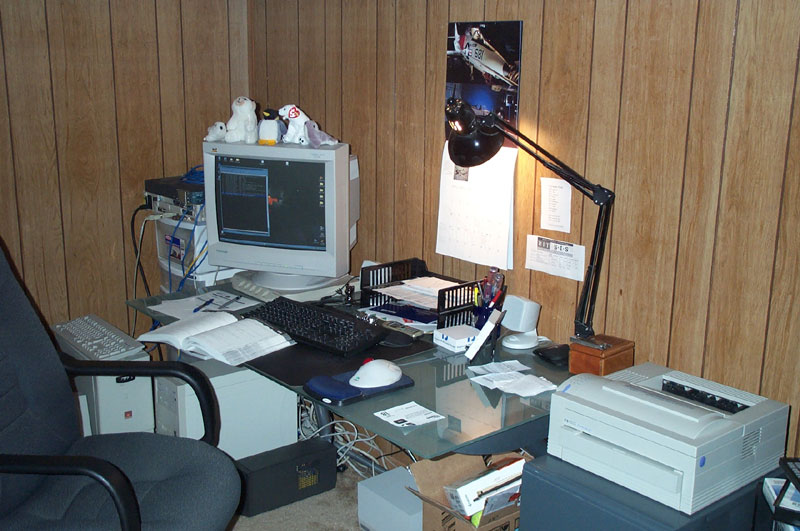
\includegraphics[width=8.33333in,height=\textheight,keepaspectratio]{images/old_desktop.jpg}

}

\caption{\label{fig-olddesk}Setup usual de um computador pessoal no
começo dos anos 2000. Fonte: \emph{Wikimedia Commons}}

\end{figure}%

Neste capítulo, serão apresentados os principais mecanismos de decisão e
repetição em Python: a construção de expressões booleanas, o uso de
estruturas condicionais, os laçõs de repetição (\emph{loops}, em
inglês), instruções de controle que indicam um ponto de parada ou
continuação do código, e as chamadas \emph{list comprehensions} como
forma compacta de iteração. Esses instrumentos formam o núcleo da
programação imperativa no Python e são indispensáveis para qualquer
aplicação computacional em Economia e análise de dados.

\subsection{Pré-requisitos}\label{pruxe9-requisitos-4}

Embora as funções e estruturas necessárias para a implementação de
expressões condicionais e \emph{loops} no Python sejam nativas na
linguagem, para algumas das aplicações utilizaremos um dos pacotes
externos que nos permitem trabalhar com números aleatórios, o
\emph{NumPy}. Além disso, em alguma aplicações utilizaremos o pacote
\emph{time} para contagem de tempo de máquina.

\begin{itemize}
\tightlist
\item
  \texttt{numpy}
\item
  \texttt{time}
\end{itemize}

\begin{Shaded}
\begin{Highlighting}[]
\ImportTok{import}\NormalTok{ numpy }\ImportTok{as}\NormalTok{ np}
\ImportTok{import}\NormalTok{ time }
\end{Highlighting}
\end{Shaded}

\section{Execução condicional}\label{execuuxe7uxe3o-condicional}

\subsection{Expressões booleanas}\label{expressuxf5es-booleanas}

Antes de conseguirmos controlar o fluxo de execução, é preciso aprender
a definir condições através das expressões booleanas. Essas expressões
exprimem condições e comparações que resultam em um valor booleano,
\emph{True} ou \emph{False}, e são resultado da combinação entre
operadores relacionais, que comparam valores, e operadores lógicos, que
nos permitem encadear comparações. Os operadores relacionais utilizados
na linguagem são:

\begin{itemize}
\tightlist
\item
  \textbf{x == y}: x é igual a y
\item
  \textbf{x != y}: x não é igual a y
\item
  \textbf{x \textgreater{} y}: x é maior que y
\item
  \textbf{x \textless{} y}: x é menor que y
\item
  \textbf{x \textgreater= y}: x é maior ou igual a y
\item
  \textbf{x \textless= y}: x é menor ou igual a y
\end{itemize}

Os exemplos a seguir usam o operador de igualdade para comparara dois
operandos quaisquer, que podem ser simples valores ou mesmo objetos.

\begin{Shaded}
\begin{Highlighting}[]
\DecValTok{5} \OperatorTok{==} \DecValTok{5}
\end{Highlighting}
\end{Shaded}

\begin{verbatim}
True
\end{verbatim}

\begin{Shaded}
\begin{Highlighting}[]
\DecValTok{5} \OperatorTok{==} \DecValTok{6}
\end{Highlighting}
\end{Shaded}

\begin{verbatim}
False
\end{verbatim}

\begin{Shaded}
\begin{Highlighting}[]
\NormalTok{lista1 }\OperatorTok{=}\NormalTok{ [}\DecValTok{1}\NormalTok{,}\DecValTok{2}\NormalTok{,}\DecValTok{3}\NormalTok{,}\DecValTok{4}\NormalTok{,}\DecValTok{5}\NormalTok{]}
\NormalTok{lista2 }\OperatorTok{=}\NormalTok{ [}\DecValTok{5}\NormalTok{,}\DecValTok{4}\NormalTok{,}\DecValTok{3}\NormalTok{,}\DecValTok{2}\NormalTok{,}\DecValTok{1}\NormalTok{]}

\NormalTok{lista1 }\OperatorTok{==}\NormalTok{ lista2}
\end{Highlighting}
\end{Shaded}

\begin{verbatim}
False
\end{verbatim}

Há três operadores lógicos: \texttt{and}, \texttt{or} e \texttt{not}. O
significado destes operadores é semelhante ao seu significado em inglês.
Por exemplo, \texttt{x\textgreater{}=0\ and\ x\textless{}=10} só é
verdade se x for maior que 0 e x for menor que 10.
\texttt{n\%2\ ==\ 0\ or\ n\%3\ ==\ 0} é verdadeiro se uma ou as duas
condição(ões) for(em) verdadeira(s), isto é, se o número n for divisível
por 2 ou 3 (caso você não esteja familiarizado com a divisão pelo piso e
o operador módulo, tente brincar um pouco com \texttt{//} e com
\texttt{\%}). Finalmente, o operador \texttt{not} nega uma expressão
booleana, então \texttt{not\ (x\ \textgreater{}\ y)} é verdade se
\texttt{x\ \textgreater{}\ y} for falso, isto é, se x for menor que ou
igual a y.

Falando estritamente, os operandos dos operadores lógicos devem ser
expressões booleanas, mas o Python não é muito estrito. Qualquer número
que não seja zero é interpretado como \emph{True}:

\begin{Shaded}
\begin{Highlighting}[]
\DecValTok{42} \KeywordTok{and} \VariableTok{True}
\end{Highlighting}
\end{Shaded}

\begin{verbatim}
True
\end{verbatim}

Esta flexibilidade tem sua utilidade, mas há algumas sutilezas relativas
a ela que podem ser confusas. Assim, pode ser uma boa ideia evitá-la (a
menos que você tenha certeza absoluta do que está fazendo).

\subsection{Operador condicional}\label{operador-condicional}

Para escrever programas úteis, quase sempre precisamos da capacidade de
verificar condições e mudar o comportamento do programa de acordo com
elas. Instruções condicionais nos dão esta capacidade. A forma mais
simples é a instrução \texttt{if}, que tem a seguinte sintaxe básica:

\begin{Shaded}
\begin{Highlighting}[]
\ControlFlowTok{if} \OperatorTok{\textless{}}\NormalTok{condição}\OperatorTok{\textgreater{}}\NormalTok{:}
    \OperatorTok{\textless{}}\NormalTok{instruções}\OperatorTok{\textgreater{}}
\end{Highlighting}
\end{Shaded}

A expressão booleana depois do \texttt{if} é chamada de condição. Se for
verdadeira, o código identado e presente em
\texttt{\textless{}instruções\textgreater{}} é executado. Caso o
resultado da expressão booleana em
\texttt{\textless{}condição\textgreater{}} seja \emph{False}, o código
em \texttt{\textless{}instruções\textgreater{}} não é executado e o
script segue.

\begin{Shaded}
\begin{Highlighting}[]
\NormalTok{x}\OperatorTok{=}\DecValTok{5}

\ControlFlowTok{if}\NormalTok{ x }\OperatorTok{\textgreater{}} \DecValTok{0}\NormalTok{:}
    \BuiltInTok{print}\NormalTok{(}\StringTok{\textquotesingle{}x é positivo\textquotesingle{}}\NormalTok{)}
\end{Highlighting}
\end{Shaded}

\begin{verbatim}
x é positivo
\end{verbatim}

\begin{tcolorbox}[enhanced jigsaw, bottomrule=.15mm, colframe=quarto-callout-important-color-frame, arc=.35mm, coltitle=black, titlerule=0mm, opacityback=0, colback=white, toptitle=1mm, breakable, bottomtitle=1mm, toprule=.15mm, left=2mm, leftrule=.75mm, title=\textcolor{quarto-callout-important-color}{\faExclamation}\hspace{0.5em}{Importante}, rightrule=.15mm, opacitybacktitle=0.6, colbacktitle=quarto-callout-important-color!10!white]

Uma característica muito importante da sintaxe do Python é justamente a
\textbf{identação}. Diferentemente de outras linguagens de programação,
a identação exerce papel importante aqui, já que é através dela que se
determina onde se inicia e onde termina um bloco de código, que pode ser
uma expressão condicional ou mesmo uma função, como veremos mais a
frente. Além de economizar várias chaves (``\{'' e ``\}'') -- elementos
que delimitam blocos de código em outras linguagens, como o R -- a
identação exerce um papel estético importante ao permitir uma melhor
visualização do código como um todo.

\end{tcolorbox}

Uma segunda forma de utilizar a instrução \texttt{if} é a chamada
execução alternativa, na qual há duas possibilidades e a condição
determina qual será executada.

\begin{Shaded}
\begin{Highlighting}[]
\NormalTok{idade }\OperatorTok{=} \DecValTok{17}

\ControlFlowTok{if}\NormalTok{ idade }\OperatorTok{\textgreater{}=} \DecValTok{18}\NormalTok{:}
    \BuiltInTok{print}\NormalTok{(}\StringTok{\textquotesingle{}Indivíduo é maior de idade\textquotesingle{}}\NormalTok{)}
\ControlFlowTok{else}\NormalTok{:}
    \BuiltInTok{print}\NormalTok{(}\StringTok{\textquotesingle{}Indivíduo é menor de idade\textquotesingle{}}\NormalTok{)}
\end{Highlighting}
\end{Shaded}

\begin{verbatim}
Indivíduo é menor de idade
\end{verbatim}

Se o valor atribuído ao objeto idade for maior ou igual a 18, então
sabemos que o indivíduo já atingiu a maioridade e o programa exibe a
respectiva mensagem. Se a condição for falsa, o segundo conjunto de
instruções é executado, informando que o indivíuo é menor de idade. Como
a condição deve ser verdadeira ou falsa, exatamente uma das alternativas
será executada. As alternativas são chamadas de ramos (\emph{branches}),
porque são ramos no fluxo da execução.

\subsection{Condicionais encadeadas}\label{condicionais-encadeadas}

Às vezes, há mais de duas possibilidades e precisamos de mais que dois
ramos de condições. Esta forma de expressar uma operação de computação é
uma condicional encadeada.

\begin{Shaded}
\begin{Highlighting}[]
\NormalTok{x }\OperatorTok{=} \DecValTok{5}
\NormalTok{y }\OperatorTok{=} \DecValTok{6}

\ControlFlowTok{if}\NormalTok{ x }\OperatorTok{\textless{}}\NormalTok{ y:}
    \BuiltInTok{print}\NormalTok{(}\StringTok{\textquotesingle{}x é menor do que y\textquotesingle{}}\NormalTok{)}
\ControlFlowTok{elif}\NormalTok{ x }\OperatorTok{\textgreater{}}\NormalTok{ y:}
    \BuiltInTok{print}\NormalTok{(}\StringTok{\textquotesingle{}x é maior do que y\textquotesingle{}}\NormalTok{)}
\ControlFlowTok{else}\NormalTok{:}
    \BuiltInTok{print}\NormalTok{(}\StringTok{\textquotesingle{}x e y são iguais\textquotesingle{}}\NormalTok{)}
\end{Highlighting}
\end{Shaded}

\begin{verbatim}
x é menor do que y
\end{verbatim}

Novamente, exatamente um ramo será executado. Não há nenhum limite para
o número de instruções \texttt{elif}\footnote{É uma abreviação da
  expressão \emph{else if}.}. Se houver uma cláusula \texttt{else}, ela
deve estar no fim, mas não é preciso haver uma. Cada condição é
verificada em ordem. Se a primeira for falsa, a próxima é verificada, e
assim por diante. Se uma delas for verdadeira, o ramo correspondente é
executado e a instrução é encerrada. Mesmo se mais de uma condição for
verdade, só o primeiro ramo verdadeiro é executado. Em condicionais
encadeados, a ordem é importante.

\section{Repetição simples}\label{repetiuxe7uxe3o-simples}

Estruturas condicionais permitem escolher entre caminhos alternativos de
execução. No entanto, muitos problemas computacionais exigem repetir o
mesmo conjunto de instruções diversas vezes, seja para percorrer dados,
acumular resultados ou simular processos. Para isso, utilizamos
estruturas de repetição ou iteração.

De maneira um pouco mais formal, iteração significa executar o mesmo
bloco de código repetidamente, potencialmente muitas vezes. Uma
estrutura de programação que implementa a iteração é chamada de
\emph{loop}. A forma mais simples de iteração é a chamada \emph{iteração
definida}, em que o número de vezes que o bloco designado será executado
é especificado explicitamente no momento em que o \emph{loop} é
iniciado.

Para atingir o objetivo proposto pela \emph{iteração definida}
utilizaremos no Python a instrução \texttt{for}. Um loop \texttt{for}
tem duas partes: um cabeçalho especificando a iteração, que termina em
dois pontos, e um corpo identado que é executado uma vez por iteração. O
corpo pode conter qualquer número de instruções, mas o Python só
reconhecerá como parte do corpo o código que estiver identado em relação
ao cabeçalho.

No Python o \texttt{for} tem a cara abaixo

\begin{Shaded}
\begin{Highlighting}[]
\ControlFlowTok{for} \OperatorTok{\textless{}}\NormalTok{elemento}\OperatorTok{\textgreater{}} \KeywordTok{in} \OperatorTok{\textless{}}\NormalTok{objeto}\OperatorTok{\textgreater{}}\NormalTok{:}
    \OperatorTok{\textless{}}\NormalTok{instruções}\OperatorTok{\textgreater{}}
\end{Highlighting}
\end{Shaded}

Note que \texttt{\textless{}objeto\textgreater{}} em geral se refere à
uma sequência, seja ela uma lista, uma tupla, um string ou qualquer
outro objeto pelo qual seja possível percorrer. Para cada
\texttt{\textless{}elemento\textgreater{}} dentro da sequência
\texttt{\textless{}objeto\textgreater{}} o conjunto de instruções em
\texttt{\textless{}instruções\textgreater{}}será executado. Após
percorrer todos os elementos pertencentes à sequência
\texttt{\textless{}objeto\textgreater{}}, o Python para a execução do
\emph{loop}.

Imagine agora que estejamos interessados em criar um \texttt{for} loop
que printa 10 números aleatórios sorteados de uma distribuição uniforme
que vai de 0 a 1. Utilizarei para esse exemplo o objeto
\texttt{range()}, a lógica de listas e a função \texttt{uniform} do
NumPy, geradora de números aleatórios distribuídos de acordo com uma
Distribuição Uniforme padrão (definida no intervalo \([0,1]\)).

\begin{Shaded}
\begin{Highlighting}[]
\BuiltInTok{print}\NormalTok{(}\BuiltInTok{list}\NormalTok{(}\BuiltInTok{range}\NormalTok{(}\DecValTok{0}\NormalTok{,}\DecValTok{10}\NormalTok{)))}
\end{Highlighting}
\end{Shaded}

\begin{verbatim}
[0, 1, 2, 3, 4, 5, 6, 7, 8, 9]
\end{verbatim}

\begin{Shaded}
\begin{Highlighting}[]
\ControlFlowTok{for}\NormalTok{ i }\KeywordTok{in} \BuiltInTok{list}\NormalTok{(}\BuiltInTok{range}\NormalTok{(}\DecValTok{0}\NormalTok{,}\DecValTok{10}\NormalTok{)):}
    
\NormalTok{    u }\OperatorTok{=}\NormalTok{ np.random.uniform()}
    \BuiltInTok{print}\NormalTok{(u)}
\end{Highlighting}
\end{Shaded}

\begin{verbatim}
0.44274294316113716
0.6233134579543054
0.31342600070441484
0.4671510122654332
0.5307691509127416
0.12188614050090296
0.503631161863675
0.1247788688160878
0.41902373495910084
0.14170085815836753
\end{verbatim}

No \emph{loop} acima não utilizamos o elemento \texttt{i} em nenhum
momento,a lista nos serviu apenas para ditar o número de vezes que
gostaríamos de rodar o bloco de instruções abaixo do cabeçalho, no caso
10. Podemos ir um pouco além.

\begin{Shaded}
\begin{Highlighting}[]
\ControlFlowTok{for}\NormalTok{ i }\KeywordTok{in} \BuiltInTok{list}\NormalTok{(}\BuiltInTok{range}\NormalTok{(}\DecValTok{0}\NormalTok{,}\DecValTok{10}\NormalTok{)):}
    
\NormalTok{    u }\OperatorTok{=}\NormalTok{ np.random.uniform()}
\NormalTok{    string}\OperatorTok{=}\StringTok{\textquotesingle{}Essa é a iteração }\SpecialCharTok{\{:.0f\}}\StringTok{ e o número sorteado foi: }\SpecialCharTok{\{:.2f\}}\StringTok{\textquotesingle{}}

    \BuiltInTok{print}\NormalTok{(string.}\BuiltInTok{format}\NormalTok{(i,u)) }
\end{Highlighting}
\end{Shaded}

\begin{verbatim}
Essa é a iteração 0 e o número sorteado foi: 0.09
Essa é a iteração 1 e o número sorteado foi: 0.06
Essa é a iteração 2 e o número sorteado foi: 0.18
Essa é a iteração 3 e o número sorteado foi: 0.26
Essa é a iteração 4 e o número sorteado foi: 0.38
Essa é a iteração 5 e o número sorteado foi: 0.50
Essa é a iteração 6 e o número sorteado foi: 0.55
Essa é a iteração 7 e o número sorteado foi: 0.83
Essa é a iteração 8 e o número sorteado foi: 0.08
Essa é a iteração 9 e o número sorteado foi: 0.12
\end{verbatim}

Note que nesse caso utilizamos tanto o elemento \emph{iterável}
\texttt{i}, quanto o resultado de cada sorteio individual \texttt{u}.

\subsection{Iteração definida e instruções
condicionais}\label{iterauxe7uxe3o-definida-e-instruuxe7uxf5es-condicionais}

Podemos utilizar instruções condicionais dentro de um loop \texttt{for}
também. Mais do que isso, é possível utilizar esse tipo de instrução
para interromper a repetição do código, mesmo antes do Python percorrer
todos os elementos da sequência alvo. Vejamos um exemplo da brincadeira
do \emph{C e S}, em que os jogadores definem um tema e perde o primeiro
jogador a falar uma palavra relacionada ao tema que comece com a letra c
ou com a letra s.

\begin{Shaded}
\begin{Highlighting}[]
\ControlFlowTok{for}\NormalTok{ i }\KeywordTok{in}\NormalTok{ [}\StringTok{\textquotesingle{}banana\textquotesingle{}}\NormalTok{,}\StringTok{\textquotesingle{}uva\textquotesingle{}}\NormalTok{,}\StringTok{\textquotesingle{}cenoura\textquotesingle{}}\NormalTok{,}\StringTok{\textquotesingle{}melão\textquotesingle{}}\NormalTok{,}\StringTok{\textquotesingle{}salsinha\textquotesingle{}}\NormalTok{,}\StringTok{\textquotesingle{}couve{-}flor\textquotesingle{}}\NormalTok{]:}
    
\NormalTok{    cond1}\OperatorTok{=}\NormalTok{i.startswith(}\StringTok{\textquotesingle{}c\textquotesingle{}}\NormalTok{)}
\NormalTok{    cond2}\OperatorTok{=}\NormalTok{i.startswith(}\StringTok{\textquotesingle{}s\textquotesingle{}}\NormalTok{)}

    \ControlFlowTok{if}\NormalTok{ cond1 }\KeywordTok{or}\NormalTok{ cond2:}
        \ControlFlowTok{break}

    \BuiltInTok{print}\NormalTok{(i)}
\end{Highlighting}
\end{Shaded}

\begin{verbatim}
banana
uva
\end{verbatim}

Note que no caso acima, o terceiro elemento da lista
\texttt{{[}\textquotesingle{}banana\textquotesingle{},\textquotesingle{}uva\textquotesingle{},\textquotesingle{}cenoura\textquotesingle{},\textquotesingle{}melão\textquotesingle{},\textquotesingle{}salsinha\textquotesingle{},\textquotesingle{}couve-flor\textquotesingle{}{]}}
começa com a letra `c' mas os dois primeiros não. A expressão boleana
após o \texttt{if}, portanto, retorna \texttt{False} nas duas primeiras
iterações e \texttt{True} na segunda. No momento em que ela retorna
\texttt{True} a instrução \texttt{break} é executada e o loop para aí!
Dessa forma, apenas os dois primeiros termos da lista serão impressos
pela instrução \texttt{print}.

\subsection{\texorpdfstring{Usando
\emph{enumerate}}{Usando enumerate}}\label{usando-enumerate}

Até aqui, utilizamos o loop \texttt{for} para percorrer sequências
simples. Em aplicações práticas, é comum precisarmos acessar
simultaneamente o índice de um elemento. Nesse caso, pode ser útil ter
uma variável que muda em cada iteração do loop e que possibilite fazer
um controle mais direto sobre qual iteração está sendo executada em
determinado momento. Em vez de criar e incrementar uma variável você
mesmo, você pode usar a função nativa \texttt{enumerate()} para obter um
contador e o valor do objeto iterável ao mesmo tempo. Para deixar claro
como funciona a sintaxe nesse caso, vamos trabalhar em cima de uma lista
de strings.

\begin{Shaded}
\begin{Highlighting}[]
\NormalTok{str1 }\OperatorTok{=} \StringTok{\textquotesingle{}Água mole em pedra dura, tanto bate até que fura\textquotesingle{}}

\CommentTok{\# Algumas linhas de código adicionais para excluir pontuação e transformar o string em uma lista de palavras}
\NormalTok{str1 }\OperatorTok{=}\NormalTok{ str1.replace(}\StringTok{\textquotesingle{}.\textquotesingle{}}\NormalTok{,}\StringTok{\textquotesingle{}\textquotesingle{}}\NormalTok{)}
\NormalTok{str1 }\OperatorTok{=}\NormalTok{ str1.replace(}\StringTok{\textquotesingle{},\textquotesingle{}}\NormalTok{,}\StringTok{\textquotesingle{}\textquotesingle{}}\NormalTok{)}
\NormalTok{str1 }\OperatorTok{=}\NormalTok{ str1.replace(}\StringTok{\textquotesingle{}?\textquotesingle{}}\NormalTok{,}\StringTok{\textquotesingle{}\textquotesingle{}}\NormalTok{)}
\NormalTok{lista1 }\OperatorTok{=}\NormalTok{ str1.split()}

\ControlFlowTok{for}\NormalTok{ c }\KeywordTok{in}\NormalTok{ lista1:}
    \BuiltInTok{print}\NormalTok{(c)}
\end{Highlighting}
\end{Shaded}

\begin{verbatim}
Água
mole
em
pedra
dura
tanto
bate
até
que
fura
\end{verbatim}

Utilizando o \texttt{enumerate()} podemos, em uma mesma linha de código,
printar não apenas cada string individual da lista, mas também a posição
desse string dentro da lista!

\begin{Shaded}
\begin{Highlighting}[]
\ControlFlowTok{for}\NormalTok{ count,value }\KeywordTok{in} \BuiltInTok{enumerate}\NormalTok{(lista1):}
    
    \BuiltInTok{print}\NormalTok{(}\StringTok{\textquotesingle{}Elemento \textquotesingle{}}\OperatorTok{+}\BuiltInTok{str}\NormalTok{(count)}\OperatorTok{+}\StringTok{\textquotesingle{} = \textquotesingle{}}\OperatorTok{+}\NormalTok{value)}
\end{Highlighting}
\end{Shaded}

\begin{verbatim}
Elemento 0 = Água
Elemento 1 = mole
Elemento 2 = em
Elemento 3 = pedra
Elemento 4 = dura
Elemento 5 = tanto
Elemento 6 = bate
Elemento 7 = até
Elemento 8 = que
Elemento 9 = fura
\end{verbatim}

Uma outra forma de criar esses mesmos resultados seria utilizando a
função nativa \texttt{zip()}. Essa função nos permite iterar ao longo de
duas ou mais sequências ao mesmo tempo, contanto que as sequências
possuam o mesmo comprimento. Porém, seu escopo de ação é muito mais
geral já que nos permite percorrer dois objetos distintos ao mesmo
tempo, sejam quais forem esses objetos. A única obrigatoriedade é que
esses objetos tenham o mesmo tamanho.

\begin{Shaded}
\begin{Highlighting}[]
\NormalTok{professores }\OperatorTok{=}\NormalTok{ [}\StringTok{\textquotesingle{}Danilo Souza\textquotesingle{}}\NormalTok{,}\StringTok{\textquotesingle{}Danilo Souza\textquotesingle{}}\NormalTok{,}\StringTok{\textquotesingle{}Artur Viaro\textquotesingle{}}\NormalTok{,}\StringTok{\textquotesingle{}Artur Viaro\textquotesingle{}}\NormalTok{]}
\NormalTok{turmas }\OperatorTok{=}\NormalTok{ [}\StringTok{\textquotesingle{}2026101\textquotesingle{}}\NormalTok{,}\StringTok{\textquotesingle{}2026102\textquotesingle{}}\NormalTok{,}\StringTok{\textquotesingle{}2026121\textquotesingle{}}\NormalTok{,}\StringTok{\textquotesingle{}2026122\textquotesingle{}}\NormalTok{]}

\ControlFlowTok{for}\NormalTok{ p,t }\KeywordTok{in} \BuiltInTok{zip}\NormalTok{(professores,turmas):}
    
    \BuiltInTok{print}\NormalTok{(}\StringTok{\textquotesingle{}Nesse curso, a turma \textquotesingle{}}\OperatorTok{+}\NormalTok{t}\OperatorTok{+}\StringTok{\textquotesingle{} é de responsabilidade do professor \textquotesingle{}}\OperatorTok{+}\NormalTok{p)}
\end{Highlighting}
\end{Shaded}

\begin{verbatim}
Nesse curso, a turma 2026101 é de responsabilidade do professor Danilo Souza
Nesse curso, a turma 2026102 é de responsabilidade do professor Danilo Souza
Nesse curso, a turma 2026121 é de responsabilidade do professor Artur Viaro
Nesse curso, a turma 2026122 é de responsabilidade do professor Artur Viaro
\end{verbatim}

\subsection{\texorpdfstring{\emph{List
comprehensions}}{List comprehensions}}\label{list-comprehensions}

Os loops \texttt{for} permitem construir listas elemento a elemento. No
entanto, quando o objetivo é gerar uma nova lista a partir de outra
sequência seguindo uma regra simples, Python oferece uma forma
sintaticamente mais compacta: as \emph{list comprehensions}. Sua sintaxe
é bastante concisa e nos permite olhar para um exercício de iteração
através de algo parecido com uma fórmula. Imagine que estejamos
interessados em criar uma lista que contenha a parte inteira da raiz
quadrada de todo número de uma outra lista original. Usualmente faríamos
isso utilizando um loop \texttt{for}:

\begin{Shaded}
\begin{Highlighting}[]
\NormalTok{lista1 }\OperatorTok{=}\NormalTok{ [}\DecValTok{1}\NormalTok{,}\DecValTok{4}\NormalTok{,}\DecValTok{9}\NormalTok{,}\DecValTok{16}\NormalTok{,}\DecValTok{25}\NormalTok{,}\DecValTok{36}\NormalTok{,}\DecValTok{49}\NormalTok{,}\DecValTok{64}\NormalTok{,}\DecValTok{81}\NormalTok{,}\DecValTok{100}\NormalTok{,}\DecValTok{121}\NormalTok{,}\DecValTok{144}\NormalTok{,}\DecValTok{169}\NormalTok{,}\DecValTok{196}\NormalTok{,}\DecValTok{225}\NormalTok{]}
\NormalTok{lista2 }\OperatorTok{=}\NormalTok{ []}

\ControlFlowTok{for}\NormalTok{ x }\KeywordTok{in}\NormalTok{ lista1:}
\NormalTok{    lista2.append(}\BuiltInTok{int}\NormalTok{(x}\OperatorTok{**}\FloatTok{0.5}\NormalTok{))}
    
\BuiltInTok{print}\NormalTok{(lista2)}
\end{Highlighting}
\end{Shaded}

\begin{verbatim}
[1, 2, 3, 4, 5, 6, 7, 8, 9, 10, 11, 12, 13, 14, 15]
\end{verbatim}

Alternativamente, podemos utilizar \emph{list comprehensions} através da
seguinte sintaxe:

\begin{Shaded}
\begin{Highlighting}[]
\NormalTok{lista2 }\OperatorTok{=}\NormalTok{ [}\BuiltInTok{int}\NormalTok{(x}\OperatorTok{**}\FloatTok{0.5}\NormalTok{) }\ControlFlowTok{for}\NormalTok{ x }\KeywordTok{in}\NormalTok{ lista1] }

\BuiltInTok{print}\NormalTok{(lista2)}
\end{Highlighting}
\end{Shaded}

\begin{verbatim}
[1, 2, 3, 4, 5, 6, 7, 8, 9, 10, 11, 12, 13, 14, 15]
\end{verbatim}

Em termos práticos isso funciona como se fosse um loop definido dentro
de uma única linha de código. Mas se fazem a mesma coisa, qual a
diferença entre as duas formas? Vamos fazer um teste para esse exercicío
da raiz quadrada, porém para uma lista maior. Utilizaremos também a
função \texttt{time} do pacote \texttt{time} para calcular o tempo
utilizado por cada um dos métodos.

\begin{Shaded}
\begin{Highlighting}[]
\NormalTok{lista1 }\OperatorTok{=} \BuiltInTok{list}\NormalTok{(}\BuiltInTok{range}\NormalTok{(}\DecValTok{1}\NormalTok{,}\DecValTok{1000000}\NormalTok{))}

\CommentTok{\# list comprehension}
\NormalTok{start\_comp }\OperatorTok{=}\NormalTok{ time.time()}

\NormalTok{list\_comp  }\OperatorTok{=}\NormalTok{ [}\BuiltInTok{int}\NormalTok{(x}\OperatorTok{**}\FloatTok{0.5}\NormalTok{) }\ControlFlowTok{for}\NormalTok{ x }\KeywordTok{in}\NormalTok{ lista1]}

\NormalTok{end\_comp   }\OperatorTok{=}\NormalTok{ time.time()}


\CommentTok{\# loop}
\NormalTok{start\_loop }\OperatorTok{=}\NormalTok{ time.time()}

\NormalTok{list\_loop }\OperatorTok{=}\NormalTok{ []}
\ControlFlowTok{for}\NormalTok{ x }\KeywordTok{in}\NormalTok{ lista1:}
\NormalTok{    list\_loop.append(}\BuiltInTok{int}\NormalTok{(x}\OperatorTok{**}\FloatTok{0.5}\NormalTok{))  }
    
\NormalTok{end\_loop   }\OperatorTok{=}\NormalTok{ time.time()}

\NormalTok{ratio }\OperatorTok{=}\NormalTok{ (start\_loop }\OperatorTok{{-}}\NormalTok{ end\_loop) }\OperatorTok{/}\NormalTok{ (start\_comp }\OperatorTok{{-}}\NormalTok{ end\_comp)}
\end{Highlighting}
\end{Shaded}

Qual abordagem será que levou menos tempo?

\begin{Shaded}
\begin{Highlighting}[]
\BuiltInTok{print}\NormalTok{(}\StringTok{\textquotesingle{}Tempo necessário com list comprehensions: }\SpecialCharTok{\{:.4f\}}\StringTok{ segundos\textquotesingle{}}\NormalTok{.}\BuiltInTok{format}\NormalTok{(end\_comp }\OperatorTok{{-}}\NormalTok{ start\_comp))}
\BuiltInTok{print}\NormalTok{(}\StringTok{\textquotesingle{}Tempo necessário com loop: }\SpecialCharTok{\{:.4f\}}\StringTok{ segundos\textquotesingle{}}\NormalTok{.}\BuiltInTok{format}\NormalTok{(end\_loop }\OperatorTok{{-}}\NormalTok{ start\_loop))}
\BuiltInTok{print}\NormalTok{(}\StringTok{\textquotesingle{}}\CharTok{\textbackslash{}n}\StringTok{A abordagem de loop demorou }\SpecialCharTok{\{:.1\%\}}\StringTok{ mais tempo!\textquotesingle{}}\NormalTok{.}\BuiltInTok{format}\NormalTok{(ratio }\OperatorTok{{-}} \DecValTok{1}\NormalTok{))}
\end{Highlighting}
\end{Shaded}

\begin{verbatim}
Tempo necessário com list comprehensions: 0.0925 segundos
Tempo necessário com loop: 0.1261 segundos

A abordagem de loop demorou 36.4% mais tempo!
\end{verbatim}

\section{Repetição condicional}\label{repetiuxe7uxe3o-condicional}

O loop \texttt{for} é especialmente adequado quando iteramos sobre uma
sequência já definida. Entretanto, nem sempre sabemos previamente
quantas iterações serão necessárias. Em programação existem dois tipos
de iteração, indefinidas e definidas:

\begin{itemize}
\item
  Com \emph{iteração definida}, o número de vezes que o bloco designado
  será executado é especificado explicitamente no momento em que o loop
  é iniciado. É o exemplo do \texttt{for} loop com o qual trabalhamos
  anteriormente.
\item
  Com \emph{iteração indefinida}, o número de vezes que o loop é
  executado não é especificado explicitamente com antecedência. Em vez
  disso, o bloco designado é executado repetidamente enquanto alguma
  condição for atendida.
\end{itemize}

Para interação indefinida, a construção típica no Python é o loop
\texttt{while}. A forma mais simples desse loop é a seguinte:

\begin{Shaded}
\begin{Highlighting}[]
\ControlFlowTok{while} \OperatorTok{\textless{}}\NormalTok{condição}\OperatorTok{\textgreater{}}\NormalTok{:}
    \OperatorTok{\textless{}}\NormalTok{instruções}\OperatorTok{\textgreater{}}
\end{Highlighting}
\end{Shaded}

Em que \texttt{\textless{}instruções\textgreater{}} representam uma ou
mais linhas de código a serem executadas. Da mesma forma que nas outras
estruturas, a indentação determina quais linhas vão ser executadas
enquanto a expressão boleana em
\texttt{\textless{}condição\textgreater{}} for satisfeita. Quando um
loop \texttt{while} é encontrado, o primeiro passo da linguagem é
avaliar \texttt{\textless{}condição\textgreater{}}. Se for verdadeiro, o
corpo do loop é executado. Em seguida,
\texttt{\textless{}condição\textgreater{}} é verificado novamente e, se
ainda for verdadeiro, o corpo é executado novamente. Isso continua até a
expressão se tornar falsa, momento em que a execução do programa
prossegue para a primeira instrução além do corpo do loop. É comum,
dentro do corpo do loop, ter algum objeto que atualize elementos que são
avaliados na expressão booleana do loop. Por vezes, esse objeto
representa ou um determinado número máximo de iterações ou algum nível
de tolerância que é atualizado a cada nova iteração. É preciso ter muita
atenção a esse ponto para que o loop não fique rodando para
sempre.\footnote{Uma das formas de interromper à força a execução de um
  loop é por meio das teclas \texttt{Ctrl+C}.}

Veja o que acontece no exemplo abaixo:

\begin{Shaded}
\begin{Highlighting}[]
\NormalTok{n }\OperatorTok{=} \DecValTok{5}

\ControlFlowTok{while}\NormalTok{ n }\OperatorTok{\textgreater{}} \DecValTok{0}\NormalTok{:}
\NormalTok{    n }\OperatorTok{=}\NormalTok{ n}\OperatorTok{{-}}\DecValTok{1}
    \BuiltInTok{print}\NormalTok{(n)}
    
\BuiltInTok{print}\NormalTok{(}\StringTok{\textquotesingle{}}\CharTok{\textbackslash{}n}\StringTok{À partir de agora as instruções fora do loop serão executadas.\textquotesingle{}}\NormalTok{)}
\end{Highlighting}
\end{Shaded}

\begin{verbatim}
4
3
2
1
0

À partir de agora as instruções fora do loop serão executadas.
\end{verbatim}

A expressão no cabeçalho do loop é \texttt{n\ \textgreater{}\ 0}, o que
é \texttt{True} inicialmente já que 5 é um número positivo. Dentro do
corpo do loop redefinimos o valor de \texttt{n} para que seja igual ao
valor anterior de \texttt{n} menos 1, e então o novo valor de \texttt{n}
é impresso. Quando o corpo do loop termina, a execução do programa
retorna ao topo do loop na linha 2 e a expressão é avaliada novamente.
Como \texttt{n} ainda é positivo, o corpo é executado novamente. Isso
continua até \texttt{n} se tornar 0. Nesse ponto, quando a expressão é
testada, ela é falsa (0 não é maior do que 0) e o loop termina. A
execução é retomada na primeira instrução após o corpo do loop, no caso
a instrução print.

A seguir temos um loop que usa uma lista como condição. Nesse caso, o
Python entende, dentro de um contexto booleano, que a condição é
verdadeira enquanto a lista não for vazia. Neste exemplo, \texttt{a} é
uma condição verdadeira desde que a lista tenha elementos. Quando todos
os itens forem removidos com o método \texttt{.pop()} e a lista estiver
vazia, \texttt{a} será falsa e o loop terminará.

\begin{Shaded}
\begin{Highlighting}[]
\NormalTok{a }\OperatorTok{=}\NormalTok{ [}\StringTok{\textquotesingle{}Eu\textquotesingle{}}\NormalTok{,}\StringTok{\textquotesingle{}Tu\textquotesingle{}}\NormalTok{,}\StringTok{\textquotesingle{}Ele\textquotesingle{}}\NormalTok{,}\StringTok{\textquotesingle{}Nós\textquotesingle{}}\NormalTok{,}\StringTok{\textquotesingle{}Vós\textquotesingle{}}\NormalTok{,}\StringTok{\textquotesingle{}Eles\textquotesingle{}}\NormalTok{]}
\BuiltInTok{print}\NormalTok{(a)}

\ControlFlowTok{while}\NormalTok{ a:}
\NormalTok{    a.pop(}\OperatorTok{{-}}\DecValTok{1}\NormalTok{)}
    \BuiltInTok{print}\NormalTok{(a)}
\end{Highlighting}
\end{Shaded}

\begin{verbatim}
['Eu', 'Tu', 'Ele', 'Nós', 'Vós', 'Eles']
['Eu', 'Tu', 'Ele', 'Nós', 'Vós']
['Eu', 'Tu', 'Ele', 'Nós']
['Eu', 'Tu', 'Ele']
['Eu', 'Tu']
['Eu']
[]
\end{verbatim}

\subsection{Formas de Interromper um
Loop}\label{formas-de-interromper-um-loop}

Ao trabalhar com loops controlados por condição, pode surgir a
necessidade de interromper a execução antes que a condição principal
deixe de ser satisfeita. Para esses casos, Python fornece mecanismos
explícitos de interrupção. São duas as principais palavras-chave que
encerram uma iteração de loop prematuramente:

\begin{itemize}
\tightlist
\item
  A instrução \texttt{break} encerra um loop imediatamente. Já vimos
  como ela funciona no caso do \texttt{for} loop e instruções
  condicionais.
\end{itemize}

\begin{Shaded}
\begin{Highlighting}[]
\NormalTok{n }\OperatorTok{=} \DecValTok{5}

\ControlFlowTok{while}\NormalTok{ n }\OperatorTok{\textgreater{}} \DecValTok{0}\NormalTok{:}
\NormalTok{    n }\OperatorTok{=}\NormalTok{ n }\OperatorTok{{-}} \DecValTok{1}
    \ControlFlowTok{if}\NormalTok{ n }\OperatorTok{==} \DecValTok{2}\NormalTok{:}
        \ControlFlowTok{break}
    \BuiltInTok{print}\NormalTok{(n)}
    
\BuiltInTok{print}\NormalTok{(}\StringTok{\textquotesingle{}Loop ended.\textquotesingle{}}\NormalTok{)}
\end{Highlighting}
\end{Shaded}

\begin{verbatim}
4
3
Loop ended.
\end{verbatim}

\begin{itemize}
\tightlist
\item
  A instrução \texttt{continue}, por outro lado, encerra imediatamente a
  iteração atual. A execução salta para o topo do loop e a expressão de
  controle é reavaliada para determinar se o loop será executado
  novamente ou terminará.
\end{itemize}

\begin{Shaded}
\begin{Highlighting}[]
\NormalTok{n }\OperatorTok{=} \DecValTok{5}

\ControlFlowTok{while}\NormalTok{ n }\OperatorTok{\textgreater{}} \DecValTok{0}\NormalTok{:}
\NormalTok{    n }\OperatorTok{=}\NormalTok{ n }\OperatorTok{{-}} \DecValTok{1}
    \ControlFlowTok{if}\NormalTok{ n }\OperatorTok{==} \DecValTok{2}\NormalTok{:}
        \ControlFlowTok{continue}
    \BuiltInTok{print}\NormalTok{(n)}

\BuiltInTok{print}\NormalTok{(}\StringTok{\textquotesingle{}Loop ended.\textquotesingle{}}\NormalTok{)}
\end{Highlighting}
\end{Shaded}

\begin{verbatim}
4
3
1
0
Loop ended.
\end{verbatim}

Até este ponto, exploramos os blocos fundamentais que permitem controlar
decisões e repetições em um programa. O próximo passo é aplicá-los em um
problema computacional concreto. Simulações estatísticas são um exemplo
típico em que loops e estruturas condicionais são indispensáveis. Na
seção seguinte, utilizaremos esses instrumentos para ilustrar
computacionalmente o Teorema Central do Limite.

\section{Aplicação: Teorema Central do
Limite}\label{aplicauxe7uxe3o-teorema-central-do-limite}

O \emph{Teorema Central do Limite} é um resultado super importante em
estatística e com aplicações nas mais diversas áreas. Em sua formulação
mais simples, o teorema pode ser resumido pela caixa abaixo.

\begin{tcolorbox}[enhanced jigsaw, bottomrule=.15mm, colframe=quarto-callout-tip-color-frame, arc=.35mm, coltitle=black, titlerule=0mm, opacityback=0, colback=white, toptitle=1mm, breakable, bottomtitle=1mm, toprule=.15mm, left=2mm, leftrule=.75mm, title=\textcolor{quarto-callout-tip-color}{\faLightbulb}\hspace{0.5em}{Teorema Central do Limite}, rightrule=.15mm, opacitybacktitle=0.6, colbacktitle=quarto-callout-tip-color!10!white]

Suponha que estejamos amostrando de uma variável aleatória \(X\) com
média finita e igual a \(\mu\) e desvio padrão finito e igual a
\(\sigma\). Independentemente de qual seja a distribuição original de
\(X\), a distribuição da \emph{média amostral} de \(X\) aproxima-se cada
vez mais de uma distribuição normal conforme aumenta o tamanho das
amostras para o cálculo da média. Nessa caso, média e desvio padrão da
distribuição das médias amostrais são representados por:

\[\mu_{\bar{X}}=\mu\]

\[\sigma_{\bar{X}}=\frac{\sigma}{\sqrt{N}}\]

\end{tcolorbox}

Vamos apresentar uma implementação desse Teorema em várias etapas. Na
primeira etapa iremos sortear uma amostra de 10 números aleatórios entre
-40 e 40. Assumirei que a distribuição original de \(X\) é uniforme e,
portanto, utilizarei a função \texttt{uniform()} do \texttt{NumPy} para
o sorteio dos números.

\begin{Shaded}
\begin{Highlighting}[]
\NormalTok{x }\OperatorTok{=}\NormalTok{ np.random.uniform(}\OperatorTok{{-}}\DecValTok{40}\NormalTok{, }\DecValTok{40}\NormalTok{, }\DecValTok{10}\NormalTok{)}

\BuiltInTok{print}\NormalTok{(x)}
\end{Highlighting}
\end{Shaded}

\begin{verbatim}
[ 15.24408409 -19.28817157  21.24930103 -23.28594142  20.08331927
  18.68496143 -22.52349658 -22.10207207  11.45731556  -3.77981738]
\end{verbatim}

Note que se sorteamos 10 números novamente, o resultado será diferente

\begin{Shaded}
\begin{Highlighting}[]
\NormalTok{x }\OperatorTok{=}\NormalTok{ np.random.uniform(}\OperatorTok{{-}}\DecValTok{40}\NormalTok{, }\DecValTok{40}\NormalTok{, }\DecValTok{10}\NormalTok{)}

\BuiltInTok{print}\NormalTok{(x)}
\end{Highlighting}
\end{Shaded}

\begin{verbatim}
[ 23.46747211   3.5485786   15.20716277 -37.14736865  14.51179119
   8.7670591  -13.20568404  13.74138387  21.63943263 -26.50921762]
\end{verbatim}

Para tornar o nosso exemplo mais previsível, vamos usar a função
\texttt{seed}, também do \texttt{NumPy}, que faz com o que o sorteio dos
números parta do mesmo lugar e, portanto, o resultado seja o mesmo. Isso
é uma boa prática de código quando se pretende tornar os resultados
facilmente replicáveis por outras pessoas.

\begin{Shaded}
\begin{Highlighting}[]
\NormalTok{np.random.seed(}\DecValTok{1}\NormalTok{)}

\NormalTok{x }\OperatorTok{=}\NormalTok{ np.random.uniform(}\OperatorTok{{-}}\DecValTok{40}\NormalTok{, }\DecValTok{40}\NormalTok{, }\DecValTok{10}\NormalTok{)}
\BuiltInTok{print}\NormalTok{(x)}
\end{Highlighting}
\end{Shaded}

\begin{verbatim}
[ -6.63823962  17.62595948 -39.99085001 -15.81339419 -28.25952873
 -32.61291242 -25.09918309 -12.35514184  -8.25860206   3.10533872]
\end{verbatim}

\begin{Shaded}
\begin{Highlighting}[]
\NormalTok{np.random.seed(}\DecValTok{1}\NormalTok{)}

\NormalTok{x }\OperatorTok{=}\NormalTok{ np.random.uniform(}\OperatorTok{{-}}\DecValTok{40}\NormalTok{, }\DecValTok{40}\NormalTok{, }\DecValTok{10}\NormalTok{)}
\BuiltInTok{print}\NormalTok{(x)}
\end{Highlighting}
\end{Shaded}

\begin{verbatim}
[ -6.63823962  17.62595948 -39.99085001 -15.81339419 -28.25952873
 -32.61291242 -25.09918309 -12.35514184  -8.25860206   3.10533872]
\end{verbatim}

Feito o sorteio de números aleatórios, o próximo passo é tirar a média
desse conjunto de números.

\begin{Shaded}
\begin{Highlighting}[]
\BuiltInTok{print}\NormalTok{(np.mean(x))}
\end{Highlighting}
\end{Shaded}

\begin{verbatim}
-14.829655377323416
\end{verbatim}

Como vocês podem notar, a média não deu igual a zero, embora a média da
distribuição uniforme com números inteiros que vai de -40 a 40 seja
igual a 0. E aí surge a mágica do Teorema Central do Limite. Ainda que
uma amostra não tenha a média igual à média populacional, a \emph{média
das médias} vai convergindo para zero à medida em que extraímos novas
amostras e calculamos novas médias. Vamos implementar isso através de um
loop, sorteando 50 números aleatórios por amostra e primeiro com 10
amostras:

\begin{Shaded}
\begin{Highlighting}[]
\NormalTok{np.random.seed(}\DecValTok{1}\NormalTok{)}

\CommentTok{\# número de amostras}
\NormalTok{n }\OperatorTok{=} \DecValTok{10} 
\NormalTok{means }\OperatorTok{=}\NormalTok{ [] }

\ControlFlowTok{for}\NormalTok{ j }\KeywordTok{in} \BuiltInTok{list}\NormalTok{(}\BuiltInTok{range}\NormalTok{(}\DecValTok{0}\NormalTok{,n)):}
    
\NormalTok{    lista\_sorteio }\OperatorTok{=}\NormalTok{ np.random.uniform(}\OperatorTok{{-}}\DecValTok{40}\NormalTok{, }\DecValTok{40}\NormalTok{, }\DecValTok{50}\NormalTok{)}
\NormalTok{    x }\OperatorTok{=}\NormalTok{ np.mean(lista\_sorteio)}
\NormalTok{    means.append(x)}

\NormalTok{means }\OperatorTok{=}\NormalTok{ [np.}\BuiltInTok{round}\NormalTok{(elem,}\DecValTok{2}\NormalTok{) }\ControlFlowTok{for}\NormalTok{ elem }\KeywordTok{in}\NormalTok{ means]}

\BuiltInTok{print}\NormalTok{(np.mean(means))}
\end{Highlighting}
\end{Shaded}

\begin{verbatim}
0.6619999999999999
\end{verbatim}

Agora com 100 amostras e mantendo o número de 50 sorteios por amostra:

\begin{Shaded}
\begin{Highlighting}[]
\NormalTok{np.random.seed(}\DecValTok{1}\NormalTok{)}

\CommentTok{\# número de amostras}
\NormalTok{n }\OperatorTok{=} \DecValTok{100} 
\NormalTok{means }\OperatorTok{=}\NormalTok{ [] }

\NormalTok{np.random.seed(}\DecValTok{1}\NormalTok{)}

\ControlFlowTok{for}\NormalTok{ j }\KeywordTok{in} \BuiltInTok{list}\NormalTok{(}\BuiltInTok{range}\NormalTok{(}\DecValTok{0}\NormalTok{,n)):}
    
\NormalTok{    lista\_sorteio }\OperatorTok{=}\NormalTok{ np.random.uniform(}\OperatorTok{{-}}\DecValTok{40}\NormalTok{, }\DecValTok{40}\NormalTok{, }\DecValTok{50}\NormalTok{)}
\NormalTok{    x }\OperatorTok{=}\NormalTok{ np.mean(lista\_sorteio)}
\NormalTok{    means.append(x)}

\NormalTok{means }\OperatorTok{=}\NormalTok{ [np.}\BuiltInTok{round}\NormalTok{(elem,}\DecValTok{2}\NormalTok{) }\ControlFlowTok{for}\NormalTok{ elem }\KeywordTok{in}\NormalTok{ means]}

\BuiltInTok{print}\NormalTok{(np.mean(means))}
\end{Highlighting}
\end{Shaded}

\begin{verbatim}
0.024600000000000007
\end{verbatim}

A média das médias parece ter se aproximado da média amostral verdadeira
\(\mu\), que é igual a zero, conforme aumentamos de 10 para 100
amostras. Mas e se aumentarmos para 200 ou 1000 amostras? Vamos deixar
essa tentativa de aproximar a média das médias de \(\mu\) mais
automatizada:

\begin{Shaded}
\begin{Highlighting}[]
\NormalTok{np.random.seed(}\DecValTok{1}\NormalTok{)}

\NormalTok{expoentes }\OperatorTok{=}\NormalTok{ [}\DecValTok{1}\NormalTok{,}\DecValTok{2}\NormalTok{,}\DecValTok{3}\NormalTok{,}\DecValTok{4}\NormalTok{,}\DecValTok{5}\NormalTok{,}\DecValTok{6}\NormalTok{,}\DecValTok{7}\NormalTok{,}\DecValTok{8}\NormalTok{,}\DecValTok{9}\NormalTok{,}\DecValTok{10}\NormalTok{]}
\NormalTok{N }\OperatorTok{=}\NormalTok{ [}\DecValTok{2}\OperatorTok{**}\NormalTok{exp }\ControlFlowTok{for}\NormalTok{ exp }\KeywordTok{in}\NormalTok{ expoentes]}

\NormalTok{means }\OperatorTok{=}\NormalTok{ [] }

\NormalTok{np.random.seed(}\DecValTok{1}\NormalTok{)}
\ControlFlowTok{for}\NormalTok{ n }\KeywordTok{in}\NormalTok{ N:}
    
\NormalTok{    means\_atual }\OperatorTok{=}\NormalTok{ [] }
    \ControlFlowTok{for}\NormalTok{ j }\KeywordTok{in} \BuiltInTok{list}\NormalTok{(}\BuiltInTok{range}\NormalTok{(}\DecValTok{0}\NormalTok{,n)):}
        
\NormalTok{        lista\_sorteio }\OperatorTok{=}\NormalTok{ np.random.uniform(}\OperatorTok{{-}}\DecValTok{40}\NormalTok{, }\DecValTok{40}\NormalTok{, }\DecValTok{100}\NormalTok{)}
\NormalTok{        x }\OperatorTok{=}\NormalTok{ np.mean(lista\_sorteio)}
\NormalTok{        means\_atual.append(x)}
        
\NormalTok{    means.append(np.mean(means\_atual))}
\end{Highlighting}
\end{Shaded}

\begin{Shaded}
\begin{Highlighting}[]
\ControlFlowTok{for}\NormalTok{ m }\KeywordTok{in}\NormalTok{ means:}
    
    \BuiltInTok{print}\NormalTok{(np.}\BuiltInTok{round}\NormalTok{(m,}\DecValTok{2}\NormalTok{))}
\end{Highlighting}
\end{Shaded}

\begin{verbatim}
-1.17
0.92
0.37
-0.25
0.31
-0.32
0.23
-0.15
-0.06
0.03
\end{verbatim}

Olha só a convergência aí, minha gente!

Note que até aqui a gente só mostrou que a média das médias converge
para a média populacional. O Teorema, no entanto, é mais completo do que
isso. Ele diz que a distribuição da média amostral é uma Normal e, além
disso, possui aquelas características em relação à distribuição
original. Ainda precisamos de mais algumas aulas para ir além e olhar
essas outrs questões do Teorema, mas logo logo chegamos lá.

\section{Conclusão}\label{conclusuxe3o-4}

Neste capítulo, foram apresentados os principais mecanismos de controle
de fluxo em Python, responsáveis por determinar como e quando
determinadas instruções são executadas. Você aprendeu a utilizar
estruturas condicionais com base em expressões booleanas, bem como
estruturas de repetição definidas e indefinidas para executar blocos de
código múltiplas vezes. Também foram discutidos recursos de controle
fino de loops, além das \emph{list comprehensions} como forma
sinteticamente mais compacta e eficiente de realizar loops no contexto
de listas. Essas ferramentas constituem a base de praticamente qualquer
algoritmo aplicado, permitindo automatizar cálculos, implementar regras
lógicas e estruturar procedimentos repetitivos. A partir desses
fundamentos, torna-se possível organizar o código de forma mais modular
e reutilizável, tema que será desenvolvido no próximo capítulo por meio
do estudo de funções.

\section{Exercícios}\label{exercuxedcios-4}

\begin{enumerate}
\def\labelenumi{\arabic{enumi}.}
\item
  Escreva um programa que receba a lista de rendas mensais abaixo e
  classifique cada observação nas seguintes categorias:

  \begin{itemize}
  \tightlist
  \item
    Dados:
    \texttt{rendas\ =\ {[}1200,\ 3240,\ 3250,\ 7100,\ 12000,\ 5000,\ 7500,\ 1800,\ 4500{]}}
  \item
    ``Baixa renda'' caso a renda mensal seja menor do que 2 salários
    mínimos.
  \item
    ``Renda média'' caso a renda mensal esteja entre 2 e 5 salários
    mínimos.
  \item
    ``Alta renda'' caso contrário.
  \end{itemize}

  O programa deve retornar uma nova lista contendo as classificações na
  mesma ordem da lista original. Você deve utilizar as instruções
  \texttt{if} e \texttt{for}. Considere o salário mínimo de
  \(R\$ 1.621\) (valor de 2026)
\item
  Utilize o loop \texttt{while} para construir um código que realize uma
  soma infinita de uma progressão geométrica em que o primeiro termo é
  igual a \(10\) e a razão é igual a \(0.9\).Lembre-se de definir um
  critério de parada para que o loop não rode para sempre.
\item
  Escreva um programa que, a partir de uma lista de dados, percorra
  todos os elementos um a um ignorando valores negativos, interrompendo
  o loop caso encontre um número maior do que \(8\), e somando todos os
  valores processados pelo loop antes da interrupção. Aplique esse
  programa à lista
  \texttt{numeros\ =\ {[}4,7,-2,9,1,2,-10,6,-5,3,7,-0.5,12,1,3,-2{]}}.
\item
  Simule 10.000 lançamentos de um dado justo utilizando a função
  \texttt{randint} do \texttt{numpy.random}. Utilize um loop
  \texttt{for} e expressões condicionais para (i) calcular a frequência
  relativa de cada face e (ii) a média dos valores obtidos dentro da
  amostra de lançamentos.
\item
  O último teorema de \emph{Fermat} diz que não há nenhum número inteiro
  positivo \emph{a,b,c} tal que \[ a^n + b^n = c^n \]

  para quaisquer valores de n maiores do que 2.

  Use o que você aprendeu com condicionais, operações aritméticas e
  instruções print para testar se o teorema se mantém, dada a lista de
  números inteiros abaixo. Note que ao fim de cada iteração, o programa
  deve exibir ``Holy smokes! Fermat was wrong'' caso o teorema não valha
  e ``Fermat was right'' caso você não tenha refutado um gênio dos
  tempos modernos.

  \begin{itemize}
  \tightlist
  \item
    \texttt{a\ =\ {[}1,2,3,4,5,6,7,8,9,10{]}}
  \item
    \texttt{b\ =\ {[}1,2,3,4,5,6,7,8,9,10{]}}
  \item
    \texttt{n\ =\ {[}3,4,5,6,7,8,9,10,37,52,89,100{]}}
  \end{itemize}
\end{enumerate}

\chapter{Funções}\label{sec-funcoes}

\section{Introdução}\label{introduuxe7uxe3o-5}

Até aqui, os programas escritos consistem em sequências de instruções,
condicionais e laços que manipulam objetos como números, listas e
dicionários. Essa forma é suficiente para resolver problemas simples,
mas rapidamente se torna difícil de manter quando o código cresce ou
quando a mesma lógica precisa ser reutilizada várias vezes.

Funções são o principal mecanismo de abstração em programação. Elas
permitem encapsular um conjunto de instruções sob um nome, definir
claramente quais informações entram e quais resultados saem, e separar a
lógica interna da interface externa. Em termos computacionais, funções
organizam o fluxo de execução, delimitam escopos de variáveis e tornam
explícita a transformação entre \emph{inputs} e \emph{outputs} --
conceito central também em Economia, onde frequentemente modelamos
relações funcionais entre variáveis.

\begin{figure}

\centering{

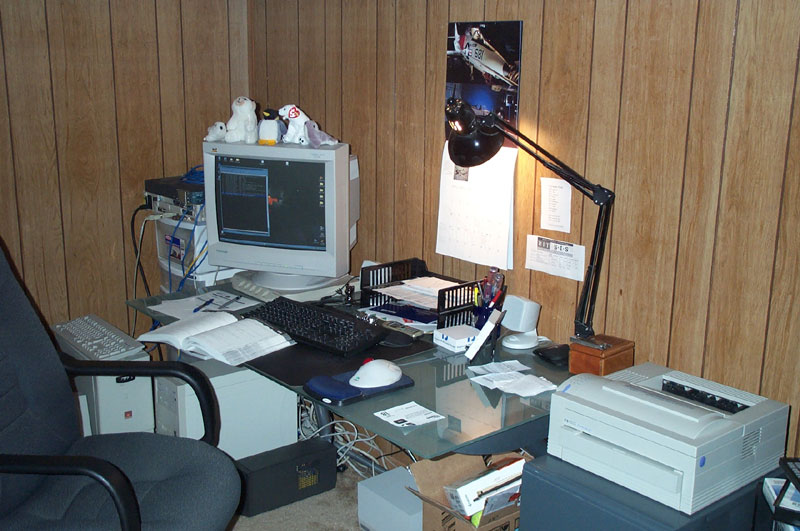
\includegraphics[width=8.33333in,height=\textheight,keepaspectratio]{images/old_desktop.jpg}

}

\caption{\label{fig-olddesk}Setup usual de um computador pessoal no
começo dos anos 2000. Fonte: \emph{Wikimedia Commons}}

\end{figure}%

Neste capítulo, o objetivo é compreender o papel das funções como
ferramenta de organização, reutilização e clareza lógica. Ao final, o
aluno deverá ser capaz de estruturar programas de forma modular e
compreender como funções são usadas extensivamente nas bibliotecas
científicas que serão estudadas nas próximas aulas.

\subsection{Pré-requisitos}\label{pruxe9-requisitos-5}

Para trabalhar com funções e todas as suas funcionalidades, utilizaremos
dois pacotes externos:

\begin{itemize}
\tightlist
\item
  \texttt{numpy}
\item
  \texttt{time}
\end{itemize}

\begin{Shaded}
\begin{Highlighting}[]
\ImportTok{import}\NormalTok{ numpy }\ImportTok{as}\NormalTok{ np}
\ImportTok{import}\NormalTok{ time}
\end{Highlighting}
\end{Shaded}

\section{Importância da
modularização}\label{importuxe2ncia-da-modularizauxe7uxe3o}

Até aqui, os programas foram escritos como sequências lineares de
instruções executadas de cima para baixo. Esse modelo é suficiente
quando resolvemos um único problema específico com um único conjunto de
dados. No entanto, ele se torna inadequado quando precisamos aplicar a
mesma regra várias vezes ou quando o código começa a crescer.

Considere o seguinte exemplo. Suponha que desejamos calcular a média de
diferentes conjuntos de notas:

\begin{Shaded}
\begin{Highlighting}[]
\NormalTok{notas1 }\OperatorTok{=}\NormalTok{ [}\FloatTok{7.5}\NormalTok{, }\FloatTok{8.0}\NormalTok{, }\FloatTok{6.5}\NormalTok{]}
\NormalTok{media1 }\OperatorTok{=} \BuiltInTok{sum}\NormalTok{(notas1) }\OperatorTok{/} \BuiltInTok{len}\NormalTok{(notas1)}
\BuiltInTok{print}\NormalTok{(media1)}

\NormalTok{notas2 }\OperatorTok{=}\NormalTok{ [}\FloatTok{9.0}\NormalTok{, }\FloatTok{8.5}\NormalTok{, }\FloatTok{7.0}\NormalTok{]}
\NormalTok{media2 }\OperatorTok{=} \BuiltInTok{sum}\NormalTok{(notas2) }\OperatorTok{/} \BuiltInTok{len}\NormalTok{(notas2)}
\BuiltInTok{print}\NormalTok{(media2)}
\end{Highlighting}
\end{Shaded}

\begin{verbatim}
7.333333333333333
8.166666666666666
\end{verbatim}

O código funciona, mas a regra de cálculo aparece repetida. Se
decidirmos alterar o critério -- por exemplo, aplicar um ajuste ou
excluir a menor nota -- será necessário modificar todas as ocorrências
manualmente. Esse padrão aumenta a probabilidade de erro e dificulta a
manutenção. O problema não está no cálculo em si, mas na forma como ele
está organizado. Estamos misturando duas coisas distintas: os dados, que
variam, e a regra de transformação, que permanece a mesma. Uma solução
mais robusta é separar essas duas dimensões.

É aqui que entram as funções, que nos permitem encapsular determinado
conjunto de instruções e nomeá-los. Assim, basta chamar a função pelo
seu nome para aplicar em certo conjunto de dados o mesmo conjunto de
instruções. O uso de funções introduz o conceito de modularização. Em
vez de escrever um bloco contínuo de instruções, passamos a estruturar o
programa como um conjunto de módulos (funções), cada um responsável por
uma transformação específica entre entrada e saída. Do ponto de vista
computacional, isso significa que isolamos partes do código, reduzimos
redundância e tornamos explícita a relação entre argumentos recebidos e
valores retornados.

A partir desse ponto, o objetivo é compreender formalmente como funções
são definidas, como recebem argumentos e como retornam resultados. O
foco deixa de ser apenas executar comandos e passa a ser estruturar
programas de forma lógica e reutilizável.

\section{O que é uma função?}\label{o-que-uxe9-uma-funuxe7uxe3o}

Formalmente, no contexto das linguagens de programação, uma função é uma
sequência nomeada de instruções, que executa algum tipo de operação
específica mas não necessariamente numérica, como é o caso das funções
matemáticas. A ideia essencial por trás de uma função é a de juntar
algumas tarefas comuns ou repetidas e criar uma função para que, em vez
de escrever o mesmo código várias vezes, possamos chama-la pelo nome e
reutilizar o conjunto de instruções nela contida sempre que necessário.

Caso o objetivo de dividir um programa em funções ainda não tenha ficado
claro, saiba que:

\begin{itemize}
\item
  Criar uma nova função dá a oportunidade de nomear um grupo de
  instruções, o que deixa o seu programa mais fácil de ler e de depurar.
\item
  As funções podem tornar um programa menor, eliminando o código
  repetitivo. Depois, caso precise fazer alguma alteração, basta fazê-la
  em um lugar só.
\item
  Dividir um programa longo em funções permite depurar as partes uma de
  cada vez e então reuni-las em um conjunto funcional.
\item
  As funções bem projetadas muitas vezes são úteis para muitos
  programas. Uma vez escritas e depuradas, você pode reutilizar as
  funções em programas fora daquele para o qual elas foram originalmente
  construídas.
\end{itemize}

Existem várias funções nativas no Python (e.g., \texttt{type()} para
encontrar o tipo de um objeto) e mesmo dentro de bibliotecas com as
quais já trabalhamos um pouco (e.g., \texttt{numpy.random.uniform()}
para sortear números aleatórios de acordo com uma distribuição
uniforme). À partir de agora veremos como podemos criar nossas próprias
funções dentro da linguagem. No Python, a sintaxe para criar uma função
personalizada é dada por:

\begin{Shaded}
\begin{Highlighting}[]
\KeywordTok{def}\NormalTok{ nome\_da\_funcao(argumentos):}
    \OperatorTok{\textless{}}\NormalTok{instruções}\OperatorTok{\textgreater{}}    
\end{Highlighting}
\end{Shaded}

Assim como nos \emph{loops}, para definir uma nova função no Python é
preciso começar com uma palavra-chave, nesse caso \texttt{def}. O nome
que daremos à função vem logo em seguida. É através desse nome, que
chamaremos essa função em outras partes do nosso código. Entre
parênteses definimos os argumentos que a função recebe para realizar o
conjunto de instruções em \texttt{\textless{}instruções\textgreater{}}.
Note, mais uma vez, que todo o bloco de código que estiver identado e
abaixo da linha de cabeçalho da função fará parte da função.

Vejamos um exemplo simples. A função \texttt{frase\_cinema} apresentada
a seguir tem como objetivo imprimir uma das frases mais emblemáticas da
história do cinema, originalmente introduzida na série de filmes
\emph{Star Wars}, criada por George Lucas.

\begin{Shaded}
\begin{Highlighting}[]
\KeywordTok{def}\NormalTok{ frase\_cinema():}
    \BuiltInTok{print}\NormalTok{(}\StringTok{\textquotesingle{}Que a força esteja com você!\textquotesingle{}}\NormalTok{)}
\end{Highlighting}
\end{Shaded}

Note que nesse caso, o parênteses logo após o nome da função está vazio.
Isso quer dizer que essa função não recebe argumentos, apenas printa a
frase entre aspas sempre que for chamada. Para chamá-la, basta usar o
nome \texttt{frase\_cinema} seguido dos parênteses vazios:

\begin{Shaded}
\begin{Highlighting}[]
\NormalTok{frase\_cinema()}
\end{Highlighting}
\end{Shaded}

\begin{verbatim}
Que a força esteja com você!
\end{verbatim}

\section{Argumentos de uma função}\label{argumentos-de-uma-funuxe7uxe3o}

Na função anterior, não tínhamos nenhum argumento. Ou seja, toda vez que
chamarmos a função \texttt{frase\_cinema}, ela fará a mesma coisa. Pode
até ser que seja esse o objetivo, apenas economizar linhas de código. A
ideia de função, no entanto, é muito mais poderosa do que simplesmente
uma ``abreviação'' de um monte de linhas de código. A abstração
implícita no conceito de função é poderosa o suficiente para garantir
que a função retorne coisas diferentes caso você altere algum
\emph{argumento}. Vamos falar disso a seguir.

\subsection{\texorpdfstring{\emph{Keyword arguments} e \emph{default
values}}{Keyword arguments e default values}}\label{keyword-arguments-e-default-values}

Comecemos criando uma nova função \texttt{my\_func} que receba como
argumentos um nome próprio e uma localização.

\begin{Shaded}
\begin{Highlighting}[]
\KeywordTok{def}\NormalTok{ my\_func(name,place):}
\NormalTok{    strf}\OperatorTok{=}\StringTok{\textquotesingle{}Olá \textquotesingle{}}\OperatorTok{+}\NormalTok{name}\OperatorTok{+}\StringTok{\textquotesingle{}! Você é de \textquotesingle{}}\OperatorTok{+}\NormalTok{place}\OperatorTok{+}\StringTok{\textquotesingle{}?\textquotesingle{}}
    \BuiltInTok{print}\NormalTok{(strf)}

\NormalTok{my\_func(}\StringTok{\textquotesingle{}Emily\textquotesingle{}}\NormalTok{,}\StringTok{\textquotesingle{}Paris\textquotesingle{}}\NormalTok{)}
\end{Highlighting}
\end{Shaded}

\begin{verbatim}
Olá Emily! Você é de Paris?
\end{verbatim}

Ao chamar a função \texttt{my\_func}, ela combina os argumentos
\texttt{Emily} e \texttt{Paris} dentro de um único string e printa esse
string final. O que acontece, no entanto, se especificarmos o argumento
\texttt{place} primeiro e depois o \texttt{name}?

\begin{Shaded}
\begin{Highlighting}[]
\NormalTok{my\_func(}\StringTok{\textquotesingle{}Ribeirão Preto\textquotesingle{}}\NormalTok{,}\StringTok{\textquotesingle{}Roberto\textquotesingle{}}\NormalTok{)}
\end{Highlighting}
\end{Shaded}

\begin{verbatim}
Olá Ribeirão Preto! Você é de Roberto?
\end{verbatim}

Um pouco estranho, não? A razão é que nesse exemplo utilizamos os
chamados \emph{argumentos posicionais}. Ou seja, a função vai assumir
que o primeiro argumento é o \texttt{name} e o segundo é o
\texttt{place}, não importa o que tenhamos passado como argumento. Para
lidar com isso, a podemos atribuir um nome, ou \_palavra-chave, a cada
um dos argumentos. Nesse caso, será a palavra-chave, e não a posição,
que vai determinar qual o valor atribuído a cada argumento dentro da
função.

\begin{Shaded}
\begin{Highlighting}[]
\NormalTok{my\_func(place}\OperatorTok{=}\StringTok{\textquotesingle{}Ribeirão Preto\textquotesingle{}}\NormalTok{,name}\OperatorTok{=}\StringTok{\textquotesingle{}Roberto\textquotesingle{}}\NormalTok{)}
\end{Highlighting}
\end{Shaded}

\begin{verbatim}
Olá Roberto! Você é de Ribeirão Preto?
\end{verbatim}

Note que agora a posição passou a ser irrelevante porque colocamos os
nomes de cada um dos argumentos. E se quiséssemos dar ainda mais
flexibilidade à função, só especificando um subconjunto dos argumentos?
Para que isso funcione, nós precisamos especificar os
\emph{valores-padrão} dos argumentos caso eles não sejam fornecidos.
Abaixo uma função que faz exatamente isso.

\begin{Shaded}
\begin{Highlighting}[]
\KeywordTok{def}\NormalTok{ total\_calc(bill\_amount,tip\_perc}\OperatorTok{=}\DecValTok{10}\NormalTok{):}
\NormalTok{    total}\OperatorTok{=}\NormalTok{bill\_amount}\OperatorTok{*}\NormalTok{(}\DecValTok{1} \OperatorTok{+}\NormalTok{ tip\_perc}\OperatorTok{/}\DecValTok{100}\NormalTok{)}
\NormalTok{    total}\OperatorTok{=}\BuiltInTok{round}\NormalTok{(total,}\DecValTok{2}\NormalTok{)}
    \BuiltInTok{print}\NormalTok{(}\StringTok{\textquotesingle{}O valor final da sua conta foi: R$\textquotesingle{}}\NormalTok{.}\BuiltInTok{format}\NormalTok{(total))}
\end{Highlighting}
\end{Shaded}

Nesse caso, o argumento \texttt{bill\_amount} é obrigatório. Por outro
lado, o argumento \texttt{tip\_perc} vai assumir o valor 10 por padrão,
caso não seja fornecido nenhum outro valor em seu lugar quando chamarmos
a função.

\subsection{Argumentos arbitrários}\label{argumentos-arbitruxe1rios}

Após discutir o uso de \emph{keyword arguments} na definição de funções
em Python é natural avançar para uma questão relacionada: o que fazer
quando sequer sabemos, de antemão, quantos argumentos serão fornecidos?
Em outras palavras, é possível definir funções capazes de operar com um
número variável de entradas? A resposta é sim! O Python permite
construir funções que acomodam uma quantidade indefinida de argumentos,
preservando generalidade e reutilização de código. Para ilustrar essa
ideia, podemos definir uma função simples chamada \texttt{my\_var\_sum},
cuja finalidade é retornar a soma de todos os valores numéricos
recebidos na chamada, independentemente de quantos sejam.

\begin{Shaded}
\begin{Highlighting}[]
\KeywordTok{def}\NormalTok{ my\_var\_sum(}\OperatorTok{*}\NormalTok{args):}
    
    \BuiltInTok{sum} \OperatorTok{=} \DecValTok{0}
    \ControlFlowTok{for}\NormalTok{ arg }\KeywordTok{in}\NormalTok{ args:}
        \BuiltInTok{sum}\OperatorTok{=}\BuiltInTok{sum}\OperatorTok{+}\NormalTok{arg}
        
    \BuiltInTok{print}\NormalTok{(}\StringTok{\textquotesingle{}A soma total dos números fornecidos é igual a: \textquotesingle{}}\OperatorTok{+}\BuiltInTok{str}\NormalTok{(}\BuiltInTok{sum}\NormalTok{))}
\end{Highlighting}
\end{Shaded}

Observe como a definição da função agora tem \texttt{*args} ao invés de
argumentos nomeados. No corpo da função, fazemos um loop em
\texttt{args} até usarmos todos os argumentos. A função
\texttt{my\_var\_sum} retorna a soma de todos os números passados como
argumentos. Olha só o que acontece quando chamamos a função com
diferentes números de argumentos:

\begin{Shaded}
\begin{Highlighting}[]
\NormalTok{my\_var\_sum(}\DecValTok{99}\NormalTok{,}\DecValTok{10}\NormalTok{,}\DecValTok{54}\NormalTok{,}\DecValTok{23}\NormalTok{)}
\NormalTok{my\_var\_sum(}\DecValTok{9}\NormalTok{,}\DecValTok{87}\NormalTok{)}
\NormalTok{my\_var\_sum(}\DecValTok{5}\NormalTok{,}\DecValTok{21}\NormalTok{,}\DecValTok{36}\NormalTok{,}\DecValTok{79}\NormalTok{,}\DecValTok{45}\NormalTok{,}\DecValTok{65}\NormalTok{)}
\NormalTok{my\_var\_sum(}\DecValTok{1}\NormalTok{)}
\end{Highlighting}
\end{Shaded}

\begin{verbatim}
A soma total dos números fornecidos é igual a: 186
A soma total dos números fornecidos é igual a: 96
A soma total dos números fornecidos é igual a: 251
A soma total dos números fornecidos é igual a: 1
\end{verbatim}

Mas e se eu quiser passar não apenas uma sequência de valores, mas uma
sequência de valores com nomes? Não se preocupe, existe uma
possibilidade de fazer isso, usando o \texttt{**kwargs} na definição dos
argumentos.

Qual é a diferença entre \texttt{*args} e \texttt{**kwargs}? A diferença
é que você vai passar uma sequência de tamanho arbitrário de parâmetros,
cada um deles nomeado. Nesse caso, o Python entende os elementos em
\texttt{**kwargs} como parte de um dicionário. Cada elemento passado é
um par chave-valor, e dentro da função você tem que desempacotar o valor
da chave. Vamos seguir alguns exemplos.

\begin{Shaded}
\begin{Highlighting}[]
\KeywordTok{def}\NormalTok{ myFun(}\OperatorTok{**}\NormalTok{kwargs):}
    
    \ControlFlowTok{for}\NormalTok{ key, value }\KeywordTok{in}\NormalTok{ kwargs.items():}
        \BuiltInTok{print}\NormalTok{(key}\OperatorTok{+}\StringTok{\textquotesingle{} == \textquotesingle{}}\OperatorTok{+}\NormalTok{value)}
  
\NormalTok{myFun(first}\OperatorTok{=}\StringTok{\textquotesingle{}Geeks\textquotesingle{}}\NormalTok{, mid}\OperatorTok{=}\StringTok{\textquotesingle{}for\textquotesingle{}}\NormalTok{, last}\OperatorTok{=}\StringTok{\textquotesingle{}Geeks\textquotesingle{}}\NormalTok{)}
\end{Highlighting}
\end{Shaded}

\begin{verbatim}
first == Geeks
mid == for
last == Geeks
\end{verbatim}

Podemos misturar os tipos de argumentos (posicionais versus
\texttt{*args}/\texttt{*kwargs})? Sim!

\begin{Shaded}
\begin{Highlighting}[]
\KeywordTok{def}\NormalTok{ myFun(arg1, }\OperatorTok{**}\NormalTok{kwargs):}
    
    \ControlFlowTok{for}\NormalTok{ key, value }\KeywordTok{in}\NormalTok{ kwargs.items():}
        \BuiltInTok{print}\NormalTok{(arg1}\OperatorTok{+}\NormalTok{key}\OperatorTok{+}\StringTok{\textquotesingle{} == \textquotesingle{}}\OperatorTok{+}\NormalTok{value)}
  
\NormalTok{myFun(}\StringTok{"Hi {-} "}\NormalTok{, first}\OperatorTok{=}\StringTok{\textquotesingle{}Geeks\textquotesingle{}}\NormalTok{, mid}\OperatorTok{=}\StringTok{\textquotesingle{}for\textquotesingle{}}\NormalTok{, last}\OperatorTok{=}\StringTok{\textquotesingle{}Geeks\textquotesingle{}}\NormalTok{)}
\end{Highlighting}
\end{Shaded}

\begin{verbatim}
Hi - first == Geeks
Hi - mid == for
Hi - last == Geeks
\end{verbatim}

\subsection{Execução condicional dentro de uma
função}\label{execuuxe7uxe3o-condicional-dentro-de-uma-funuxe7uxe3o}

As funções podem retornar objetos booleanos também, o que pode ser
conveniente para esconder testes complicados dentro de uma função. Por
exemplo:

\begin{Shaded}
\begin{Highlighting}[]
\KeywordTok{def}\NormalTok{ is\_divisible(x, y):}
    
    \ControlFlowTok{if}\NormalTok{ x }\OperatorTok{\%}\NormalTok{ y }\OperatorTok{==} \DecValTok{0}\NormalTok{:}
        \BuiltInTok{print}\NormalTok{(}\VariableTok{True}\NormalTok{)}
    \ControlFlowTok{else}\NormalTok{:}
        \BuiltInTok{print}\NormalTok{(}\VariableTok{False}\NormalTok{)}
    
\NormalTok{is\_divisible(}\DecValTok{6}\NormalTok{, }\DecValTok{4}\NormalTok{)}
\end{Highlighting}
\end{Shaded}

\begin{verbatim}
False
\end{verbatim}

\subsection{Iteração dentro de uma
função}\label{iterauxe7uxe3o-dentro-de-uma-funuxe7uxe3o}

Da mesma forma que podemos ter condições lógicas dentro da função,
podemos ter blocos de repetição (\texttt{for} e \texttt{while}) dentro
da função, assim como no caso de argumentos arbitrários. Vamos olhar
para um outro exemplo em que a função recebe uma lista de strings como
argumento e faz operações em cada um dos elementos, um a um:

\begin{Shaded}
\begin{Highlighting}[]
\NormalTok{states }\OperatorTok{=}\NormalTok{ [}\StringTok{\textquotesingle{} Alabama \textquotesingle{}}\NormalTok{,}\StringTok{\textquotesingle{}Georgia!\textquotesingle{}}\NormalTok{,}\StringTok{\textquotesingle{}Georgia\textquotesingle{}}\NormalTok{,}\StringTok{\textquotesingle{}georgia\textquotesingle{}}\NormalTok{,}\StringTok{\textquotesingle{}FlOrIda\textquotesingle{}}\NormalTok{,}\StringTok{\textquotesingle{}south carolina\#\#\textquotesingle{}}\NormalTok{,}\StringTok{\textquotesingle{}West virginia?\textquotesingle{}}\NormalTok{]}

\KeywordTok{def}\NormalTok{ clean\_strings(lista\_strings):}
\NormalTok{    result}\OperatorTok{=}\NormalTok{[]}
    
    \ControlFlowTok{for}\NormalTok{ value }\KeywordTok{in}\NormalTok{ lista\_strings:}
\NormalTok{        value }\OperatorTok{=}\NormalTok{ value.strip()}
\NormalTok{        value }\OperatorTok{=}\NormalTok{ value.title()}
\NormalTok{        value }\OperatorTok{=}\NormalTok{ value.replace(}\StringTok{\textquotesingle{}\#\textquotesingle{}}\NormalTok{,}\StringTok{\textquotesingle{}\textquotesingle{}}\NormalTok{)}
\NormalTok{        value }\OperatorTok{=}\NormalTok{ value.replace(}\StringTok{\textquotesingle{}?\textquotesingle{}}\NormalTok{,}\StringTok{\textquotesingle{}\textquotesingle{}}\NormalTok{)}
\NormalTok{        value }\OperatorTok{=}\NormalTok{ value.replace(}\StringTok{\textquotesingle{}!\textquotesingle{}}\NormalTok{,}\StringTok{\textquotesingle{}\textquotesingle{}}\NormalTok{)}
\NormalTok{        result.append(value)}
    
    \BuiltInTok{print}\NormalTok{(result)}

\BuiltInTok{print}\NormalTok{(states)}
\NormalTok{clean\_strings(states)}
\end{Highlighting}
\end{Shaded}

\begin{verbatim}
[' Alabama ', 'Georgia!', 'Georgia', 'georgia', 'FlOrIda', 'south carolina##', 'West virginia?']
['Alabama', 'Georgia', 'Georgia', 'Georgia', 'Florida', 'South Carolina', 'West Virginia']
\end{verbatim}

Conforme as funções se tornam mais complexas, incorporando lógica
condicional e laços, torna-se fundamental entender como extrair
resultados de funções. Até aqui, muitos exemplos mostraram funções que
apenas imprimem valores; na seção seguinte analisaremos o papel do
comando \texttt{return} e sua importância na prática.

\section{Valor de retorno de uma
função}\label{valor-de-retorno-de-uma-funuxe7uxe3o}

A instrução \texttt{return} é o mecanismo pelo qual uma função envia um
resultado de volta ao ponto em que foi chamada. Do ponto de vista
lógico, uma função representa uma transformação entre entradas
(argumentos) e saídas (valores retornados). O \texttt{return} explicita
qual é essa saída e, além disso, encerra imediatamente a execução da
função no momento em que é encontrado. Se não houver nenhuma instrução
\texttt{return} no corpo da função, ou se for utilizado apenas
\texttt{return} sem valor explícito, o Python devolve automaticamente o
valor especial \texttt{None}.

Um dos erros mais frequentes entre iniciantes é confundir \texttt{print}
com \texttt{return}. Embora ambos possam produzir algo visível na tela,
eles têm naturezas completamente distintas. Enquanto o \texttt{print}
apenas envia uma representação do valor para a saída padrão (normalmente
o terminal), o \texttt{return} produz um valor que pode ser armazenado
em uma variável, reutilizado em cálculos ou passado como argumento para
outra função.

Vejamos um exemplo de uma função que calcula a raiz quadrada de um
número:

\begin{Shaded}
\begin{Highlighting}[]
\KeywordTok{def}\NormalTok{ raiz1(x):}
\NormalTok{    fx }\OperatorTok{=}\NormalTok{ x}\OperatorTok{**}\FloatTok{0.5}
    \BuiltInTok{print}\NormalTok{(fx)}

\NormalTok{y }\OperatorTok{=}\NormalTok{ raiz1(}\DecValTok{100}\NormalTok{)}
\BuiltInTok{print}\NormalTok{(y)}
\end{Highlighting}
\end{Shaded}

\begin{verbatim}
10.0
None
\end{verbatim}

Nesse caso, a função imprime o valor calculado, mas não o retorna. Como
não há \texttt{return}, o valor devolvido por \texttt{raiz1} é
\texttt{None}. Assim, a variável y passa a armazenar \texttt{None}, e é
exatamente isso que será impresso na última linha. Se substituirmos a
instrução de impressão pela instrução de retorno, o comportamento muda
estruturalmente:

\begin{Shaded}
\begin{Highlighting}[]
\KeywordTok{def}\NormalTok{ raiz2(x):}
\NormalTok{    fx }\OperatorTok{=}\NormalTok{ x}\OperatorTok{**}\FloatTok{0.5}
    \ControlFlowTok{return}\NormalTok{ fx}

\NormalTok{y }\OperatorTok{=}\NormalTok{ raiz2(}\DecValTok{100}\NormalTok{)}
\BuiltInTok{print}\NormalTok{(y)}
\end{Highlighting}
\end{Shaded}

\begin{verbatim}
10.0
\end{verbatim}

Agora a função devolve o valor numérico calculado. A variável y armazena
esse valor, que pode ser reutilizado em outras operações. A função passa
a se comportar como uma transformação matemática: recebe um número e
devolve outro. Essa distinção torna-se ainda mais clara quando tentamos
usar o resultado em outra operação numérica:

\begin{Shaded}
\begin{Highlighting}[]
\NormalTok{z }\OperatorTok{=}\NormalTok{ raiz1(}\DecValTok{100}\NormalTok{) }\OperatorTok{+} \DecValTok{5}
\BuiltInTok{print}\NormalTok{(z)}
\end{Highlighting}
\end{Shaded}

\begin{verbatim}
10.0
\end{verbatim}

\begin{Highlighting}
\textcolor{black}{TypeError: unsupported operand type(s) for +: 'NoneType' and 'int'}
\textcolor{black}{}\textcolor{QuartoInternalColor4}{---------------------------------------------------------------------------}\textcolor{QuartoInternalColor2}{}
\textcolor{QuartoInternalColor2}{}\textcolor{QuartoInternalColor4}{TypeError}\textcolor{QuartoInternalColor2}{                                 Traceback (most recent call last)}
\textcolor{QuartoInternalColor2}{}\textcolor{QuartoInternalColor1}{Cell}\textcolor{QuartoInternalColor2}{}\textcolor{QuartoInternalColor1}{ }\textcolor{QuartoInternalColor2}{}\textcolor{QuartoInternalColor3}{In[17]}\textcolor{QuartoInternalColor2}{}\textcolor{QuartoInternalColor3}{, line 1}\textcolor{QuartoInternalColor2}{}
\textcolor{QuartoInternalColor2}{}\textcolor{QuartoInternalColor3}{----> }\textcolor{QuartoInternalColor2}{}\textcolor{QuartoInternalColor3}{1}\textcolor{QuartoInternalColor2}{ z = }\textcolor{QuartoInternalColor2}{raiz1}\textcolor{QuartoInternalColor2}{}\textcolor{QuartoInternalColor2}{(}\textcolor{QuartoInternalColor2}{}\textcolor{QuartoInternalColor2}{100}\textcolor{QuartoInternalColor2}{}\textcolor{QuartoInternalColor2}{)}\textcolor{QuartoInternalColor2}{}\textcolor{QuartoInternalColor2}{ }\textcolor{QuartoInternalColor2}{}\textcolor{QuartoInternalColor2}{+}\textcolor{QuartoInternalColor2}{}\textcolor{QuartoInternalColor2}{ }\textcolor{QuartoInternalColor2}{}\textcolor{QuartoInternalColor2}{5}\textcolor{QuartoInternalColor2}{}
\textcolor{QuartoInternalColor2}{}\textcolor{QuartoInternalColor3}{      2}\textcolor{QuartoInternalColor2}{ }\textcolor{QuartoInternalColor7}{print}\textcolor{QuartoInternalColor2}{(z)}
\textcolor{QuartoInternalColor2}{}\textcolor{QuartoInternalColor4}{TypeError}\textcolor{QuartoInternalColor2}{: unsupported operand type(s) for +: 'NoneType' and 'int'}
\end{Highlighting}

O código acima gera erro porque \texttt{raiz1(100)} devolve
\texttt{None}, e não é possível somar None com um número. Já no caso da
função que utiliza a instrução de retorno, a operação funciona
normalmente:

\begin{Shaded}
\begin{Highlighting}[]
\NormalTok{z }\OperatorTok{=}\NormalTok{ raiz2(}\DecValTok{100}\NormalTok{) }\OperatorTok{+} \DecValTok{5}
\BuiltInTok{print}\NormalTok{(z)}
\end{Highlighting}
\end{Shaded}

\begin{verbatim}
15.0
\end{verbatim}

Em programação científica e análise de dados, quase sempre desejamos
funções que retornem valores, pois esses resultados serão encadeados em
outras operações, armazenados em estruturas de dados ou utilizados em
rotinas subsequentes. A impressão na tela é útil para depuração ou
visualização intermediária, mas não substitui o mecanismo formal de
retorno. Em termos conceituais, a diferença pode ser resumida da
seguinte forma: funções que usam apenas print produzem efeitos; funções
que utilizam return produzem valores.

\subsection{Expectativa de vida de variáveis dentro da
função}\label{expectativa-de-vida-de-variuxe1veis-dentro-da-funuxe7uxe3o}

Quando você cria uma variável dentro de uma função ela é local, ou seja,
só existe dentro da própria função. Por exemplo:

\begin{Shaded}
\begin{Highlighting}[]
\KeywordTok{def}\NormalTok{ concat\_strings(str1,str2):}
    
\NormalTok{    texto\_concatenado }\OperatorTok{=}\NormalTok{ str1 }\OperatorTok{+} \StringTok{\textquotesingle{} \textquotesingle{}} \OperatorTok{+}\NormalTok{ str2}
    \BuiltInTok{print}\NormalTok{(texto\_concatenado)}
    
\NormalTok{texto1 }\OperatorTok{=} \StringTok{\textquotesingle{}Que a força esteja com você,\textquotesingle{}}
\NormalTok{texto2 }\OperatorTok{=} \StringTok{\textquotesingle{}jovem Padawan.\textquotesingle{}}

\NormalTok{concat\_strings(texto1,texto2)}
\end{Highlighting}
\end{Shaded}

\begin{verbatim}
Que a força esteja com você, jovem Padawan.
\end{verbatim}

Essa função recebe dois argumentos, concatena-os e exibe o resultado em
uma única linha de texto. No entanto, assim que a função é encerrada, a
variável \texttt{texto\_concatenado} é deletada. O que acontece se
tentarmos acessá-la?

\begin{Shaded}
\begin{Highlighting}[]
\BuiltInTok{print}\NormalTok{(texto\_concatenado)}
\end{Highlighting}
\end{Shaded}

\begin{Highlighting}
\textcolor{black}{NameError: name 'texto\_concatenado' is not defined}
\textcolor{black}{}\textcolor{QuartoInternalColor4}{---------------------------------------------------------------------------}\textcolor{QuartoInternalColor2}{}
\textcolor{QuartoInternalColor2}{}\textcolor{QuartoInternalColor4}{NameError}\textcolor{QuartoInternalColor2}{                                 Traceback (most recent call last)}
\textcolor{QuartoInternalColor2}{}\textcolor{QuartoInternalColor1}{Cell}\textcolor{QuartoInternalColor2}{}\textcolor{QuartoInternalColor1}{ }\textcolor{QuartoInternalColor2}{}\textcolor{QuartoInternalColor3}{In[20]}\textcolor{QuartoInternalColor2}{}\textcolor{QuartoInternalColor3}{, line 1}\textcolor{QuartoInternalColor2}{}
\textcolor{QuartoInternalColor2}{}\textcolor{QuartoInternalColor3}{----> }\textcolor{QuartoInternalColor2}{}\textcolor{QuartoInternalColor3}{1}\textcolor{QuartoInternalColor2}{ }\textcolor{QuartoInternalColor7}{print}\textcolor{QuartoInternalColor2}{(}\textcolor{QuartoInternalColor2}{texto\_concatenado}\textcolor{QuartoInternalColor2}{)}
\textcolor{QuartoInternalColor2}{}\textcolor{QuartoInternalColor4}{NameError}\textcolor{QuartoInternalColor2}{: name 'texto\_concatenado' is not defined}
\end{Highlighting}

Com a base conceitual de definição, argumentos e retorno consolidada,
podemos agora aplicar esses conceitos em um exemplo mais substancial. A
aplicação do Teorema Central do Limite mostrará como estruturar uma
rotina que recebe distribuições e parâmetros como argumentos e retorna
medidas agregadas de interesse. Essa transição marca o passo do conceito
para a aplicação.

\section{Aplicação: Teorema Central do
Limite}\label{aplicauxe7uxe3o-teorema-central-do-limite-1}

O primeiro passo para replicarmos, na forma de uma função, a aplicação
do Teorema Central do Limite da aula anterior é definir uma função que
recebe como argumentos a distribuição da varíavel aleatória X, o
intervalo no qual a variável está definida, o número de sorteios que
faremos em cada amostra e o número de amostras realizadas. Para tal,
definiremos a função \texttt{func\_tcl} que recebe como argumentos
nomeados \texttt{dist} (função de distribuição da variável X),
\texttt{intervalo} (suporte da variável X), \texttt{n} (número de
sorteios por amostra) e \texttt{samples} (número de amostras).

Apesar de definir valores-padrão válidos para \texttt{intervalo},
\texttt{n} e \texttt{samples}, é atribuído ao argumento \texttt{dist} um
valor padrão igual a \texttt{None}. Isso permite ao usuário ter controle
direto sobre a função de distribuição utilizada para sortear X e evitar
tornar a nossa função uma caixa preta. Assim, caso o usuário esqueça de
definir uma distribuição válida, a função retorna um erro.

Caso defina uma função de distribuição válida, a função
\texttt{func\_tcl} avança e passar a realizar a sequência de sorteios de
cada amostra e a média dentro de cada amostra através de um loop do tipo
\texttt{for}.

\begin{Shaded}
\begin{Highlighting}[]
\CommentTok{\# definição da função}
\KeywordTok{def}\NormalTok{ func\_tcl(dist}\OperatorTok{=}\VariableTok{None}\NormalTok{,intervalo}\OperatorTok{=}\NormalTok{(}\DecValTok{0}\NormalTok{,}\DecValTok{1}\NormalTok{),n}\OperatorTok{=}\DecValTok{100}\NormalTok{, samples}\OperatorTok{=}\DecValTok{10}\NormalTok{):}
    
    \ControlFlowTok{if}\NormalTok{ dist }\OperatorTok{==} \VariableTok{None}\NormalTok{:}
        \BuiltInTok{print}\NormalTok{(}\StringTok{\textquotesingle{}Você esqueceu de carregar uma função que defina a distribuição de X.\textquotesingle{}}\NormalTok{)}
    \ControlFlowTok{else}\NormalTok{:}
\NormalTok{        means }\OperatorTok{=}\NormalTok{ []}
        \ControlFlowTok{for}\NormalTok{ j }\KeywordTok{in} \BuiltInTok{range}\NormalTok{(}\DecValTok{0}\NormalTok{,samples):}
\NormalTok{            x\_func\_tcl }\OperatorTok{=}\NormalTok{ dist(intervalo[}\DecValTok{0}\NormalTok{],intervalo[}\DecValTok{1}\NormalTok{],n)}
\NormalTok{            mean\_x }\OperatorTok{=} \BuiltInTok{sum}\NormalTok{(x\_func\_tcl)}\OperatorTok{/}\BuiltInTok{len}\NormalTok{(x\_func\_tcl)}
            
\NormalTok{            means.append(mean\_x)}
\NormalTok{            mean\_of\_means }\OperatorTok{=} \BuiltInTok{sum}\NormalTok{(means)}\OperatorTok{/}\BuiltInTok{len}\NormalTok{(means)}
        
        \ControlFlowTok{return}\NormalTok{ mean\_of\_means}

\CommentTok{\# comando para garantir a reprodutibilidade}
\NormalTok{np.random.seed(}\DecValTok{1}\NormalTok{)}

\CommentTok{\# uso da função}
\NormalTok{func\_tcl(dist}\OperatorTok{=}\NormalTok{np.random.uniform,intervalo}\OperatorTok{=}\NormalTok{(}\OperatorTok{{-}}\DecValTok{40}\NormalTok{,}\DecValTok{40}\NormalTok{),n}\OperatorTok{=}\DecValTok{50}\NormalTok{,samples}\OperatorTok{=}\DecValTok{10}\NormalTok{)}
\end{Highlighting}
\end{Shaded}

\begin{verbatim}
np.float64(0.662169619365357)
\end{verbatim}

Maravilha, agora a função nos retorna apenas o que é do nosso interesse:
a média das médias. Para chegar, finalmente, no mesmo resultado da aula
passada basta colocar essa função dentro de um loop.

\begin{Shaded}
\begin{Highlighting}[]
\NormalTok{expoentes }\OperatorTok{=}\NormalTok{ [}\DecValTok{1}\NormalTok{,}\DecValTok{2}\NormalTok{,}\DecValTok{3}\NormalTok{,}\DecValTok{4}\NormalTok{,}\DecValTok{5}\NormalTok{,}\DecValTok{6}\NormalTok{,}\DecValTok{7}\NormalTok{,}\DecValTok{8}\NormalTok{,}\DecValTok{9}\NormalTok{,}\DecValTok{10}\NormalTok{]}
\NormalTok{Y }\OperatorTok{=}\NormalTok{ [}\DecValTok{2}\OperatorTok{**}\NormalTok{exp }\ControlFlowTok{for}\NormalTok{ exp }\KeywordTok{in}\NormalTok{ expoentes]}

\NormalTok{means\_of\_means }\OperatorTok{=}\NormalTok{ []}

\NormalTok{np.random.seed(}\DecValTok{1}\NormalTok{)}
\ControlFlowTok{for}\NormalTok{ y }\KeywordTok{in}\NormalTok{ Y:}

\NormalTok{    mean\_of\_means }\OperatorTok{=}\NormalTok{ func\_tcl(dist}\OperatorTok{=}\NormalTok{np.random.uniform,intervalo}\OperatorTok{=}\NormalTok{(}\OperatorTok{{-}}\DecValTok{40}\NormalTok{,}\DecValTok{40}\NormalTok{),n}\OperatorTok{=}\DecValTok{100}\NormalTok{,samples}\OperatorTok{=}\NormalTok{y)}
\NormalTok{    means\_of\_means.append(mean\_of\_means)}
\end{Highlighting}
\end{Shaded}

\begin{Shaded}
\begin{Highlighting}[]
\ControlFlowTok{for}\NormalTok{ m }\KeywordTok{in}\NormalTok{ means\_of\_means:}
    
    \BuiltInTok{print}\NormalTok{(np.}\BuiltInTok{round}\NormalTok{(m,}\DecValTok{2}\NormalTok{))}
\end{Highlighting}
\end{Shaded}

\begin{verbatim}
-1.17
0.92
0.37
-0.25
0.31
-0.32
0.23
-0.15
-0.06
0.03
\end{verbatim}

\emph{Voilá}! Como exercício para casa, tente fazer alterações nessa
função de modo que ela receba não um valor com o número de amostras, mas
uma lista de números de amostras. A função deve cuspir como resultado a
lista \texttt{means\_of\_means} e não apenas o valor
\texttt{mean\_of\_means}.

Após a aplicação prática, é oportuno discutir como documentar funções de
forma que qualquer usuário (inclusive você no futuro) possa compreender
rapidamente o propósito, argumentos e comportamento de uma rotina
implementada. A próxima seção introduz docstrings como forma padrão de
documentação no Python.

\section{Documentação}\label{documentauxe7uxe3o}

Uma \emph{docstring} é uma string no início de uma função, definida pelo
usuário, que serve como documentação do que a função faz. A docstring
vem logo depois da primeira linha que define a função e é delimitada por
aspas triplas, o que permite que a string se estenda por várias linhas,
como vocês devem se lembrar. Vamos criar como exemplo uma função que
printa o tipo do objeto que é passado como argumento:

\begin{Shaded}
\begin{Highlighting}[]
\KeywordTok{def}\NormalTok{ imprime\_tipo(x):}
    
    \CommentTok{\textquotesingle{}\textquotesingle{}\textquotesingle{}}
\CommentTok{    Função criada para a matéria EAE1106 {-} Métodos Computacionais para Economia}
\CommentTok{    Objetivo: função simples que imprime o tipo do objeto recebido como argumento.}
\CommentTok{    \textquotesingle{}\textquotesingle{}\textquotesingle{}}
    
    \BuiltInTok{print}\NormalTok{(}\BuiltInTok{type}\NormalTok{(x))}
\end{Highlighting}
\end{Shaded}

Embora opcional, a documentação é uma boa prática de programação. A
menos que você consiga se lembrar qual foi o cardápio do bandejão na
semana passada, sempre documente seu código. Podemos acessar a
documentação de determinada função, nativa ou personalizada, utilizando
o atributo \texttt{\_\_doc\_\_}.

\begin{Shaded}
\begin{Highlighting}[]
\BuiltInTok{print}\NormalTok{(imprime\_tipo.\_\_doc\_\_)}
\end{Highlighting}
\end{Shaded}

\begin{verbatim}

Função criada para a matéria EAE1106 - Métodos Computacionais para Economia
Objetivo: função simples que imprime o tipo do objeto recebido como argumento.
\end{verbatim}

\begin{Shaded}
\begin{Highlighting}[]
\CommentTok{\# documentação da função nativa len()}
\BuiltInTok{print}\NormalTok{(}\BuiltInTok{len}\NormalTok{.\_\_doc\_\_)}
\end{Highlighting}
\end{Shaded}

\begin{verbatim}
Return the number of items in a container.
\end{verbatim}

\begin{Shaded}
\begin{Highlighting}[]
\CommentTok{\# documentação da função uniform() dentro do pacote NumPy}
\BuiltInTok{print}\NormalTok{(np.random.uniform.\_\_doc\_\_)}
\end{Highlighting}
\end{Shaded}

\begin{verbatim}

        uniform(low=0.0, high=1.0, size=None)

        Draw samples from a uniform distribution.

        Samples are uniformly distributed over the half-open interval
        ``[low, high)`` (includes low, but excludes high).  In other words,
        any value within the given interval is equally likely to be drawn
        by `uniform`.

        .. note::
            New code should use the `~numpy.random.Generator.uniform`
            method of a `~numpy.random.Generator` instance instead;
            please see the :ref:`random-quick-start`.

        Parameters
        ----------
        low : float or array_like of floats, optional
            Lower boundary of the output interval.  All values generated will be
            greater than or equal to low.  The default value is 0.
        high : float or array_like of floats
            Upper boundary of the output interval.  All values generated will be
            less than or equal to high.  The high limit may be included in the 
            returned array of floats due to floating-point rounding in the 
            equation ``low + (high-low) * random_sample()``.  The default value 
            is 1.0.
        size : int or tuple of ints, optional
            Output shape.  If the given shape is, e.g., ``(m, n, k)``, then
            ``m * n * k`` samples are drawn.  If size is ``None`` (default),
            a single value is returned if ``low`` and ``high`` are both scalars.
            Otherwise, ``np.broadcast(low, high).size`` samples are drawn.

        Returns
        -------
        out : ndarray or scalar
            Drawn samples from the parameterized uniform distribution.

        See Also
        --------
        randint : Discrete uniform distribution, yielding integers.
        random_integers : Discrete uniform distribution over the closed
                          interval ``[low, high]``.
        random_sample : Floats uniformly distributed over ``[0, 1)``.
        random : Alias for `random_sample`.
        rand : Convenience function that accepts dimensions as input, e.g.,
               ``rand(2,2)`` would generate a 2-by-2 array of floats,
               uniformly distributed over ``[0, 1)``.
        random.Generator.uniform: which should be used for new code.

        Notes
        -----
        The probability density function of the uniform distribution is

        .. math:: p(x) = \frac{1}{b - a}

        anywhere within the interval ``[a, b)``, and zero elsewhere.

        When ``high`` == ``low``, values of ``low`` will be returned.
        If ``high`` < ``low``, the results are officially undefined
        and may eventually raise an error, i.e. do not rely on this
        function to behave when passed arguments satisfying that
        inequality condition. The ``high`` limit may be included in the
        returned array of floats due to floating-point rounding in the
        equation ``low + (high-low) * random_sample()``. For example:

        >>> x = np.float32(5*0.99999999)
        >>> x
        np.float32(5.0)


        Examples
        --------
        Draw samples from the distribution:

        >>> s = np.random.uniform(-1,0,1000)

        All values are within the given interval:

        >>> np.all(s >= -1)
        True
        >>> np.all(s < 0)
        True

        Display the histogram of the samples, along with the
        probability density function:

        >>> import matplotlib.pyplot as plt
        >>> count, bins, ignored = plt.hist(s, 15, density=True)
        >>> plt.plot(bins, np.ones_like(bins), linewidth=2, color='r')
        >>> plt.show()

        
\end{verbatim}

Note do exemplo acima que uma docstring pode conter uma descrição
detalhada do funcionamento de uma função, inclusive com exemplos de
aplicação. Legal, né? Esse tipo de documentação também está disponível
para as bibliotecas como um todo. Isso pode nos ajudar, por exemplo, a
conhecer o conteúdo de uma determinada biblioteca.

\begin{Shaded}
\begin{Highlighting}[]
\CommentTok{\# documentação do NumPy}
\BuiltInTok{print}\NormalTok{(np.\_\_doc\_\_)}
\end{Highlighting}
\end{Shaded}

\begin{verbatim}

NumPy
=====

Provides
  1. An array object of arbitrary homogeneous items
  2. Fast mathematical operations over arrays
  3. Linear Algebra, Fourier Transforms, Random Number Generation

How to use the documentation
----------------------------
Documentation is available in two forms: docstrings provided
with the code, and a loose standing reference guide, available from
`the NumPy homepage <https://numpy.org>`_.

We recommend exploring the docstrings using
`IPython <https://ipython.org>`_, an advanced Python shell with
TAB-completion and introspection capabilities.  See below for further
instructions.

The docstring examples assume that `numpy` has been imported as ``np``::

  >>> import numpy as np

Code snippets are indicated by three greater-than signs::

  >>> x = 42
  >>> x = x + 1

Use the built-in ``help`` function to view a function's docstring::

  >>> help(np.sort)
  ... # doctest: +SKIP

For some objects, ``np.info(obj)`` may provide additional help.  This is
particularly true if you see the line "Help on ufunc object:" at the top
of the help() page.  Ufuncs are implemented in C, not Python, for speed.
The native Python help() does not know how to view their help, but our
np.info() function does.

Available subpackages
---------------------
lib
    Basic functions used by several sub-packages.
random
    Core Random Tools
linalg
    Core Linear Algebra Tools
fft
    Core FFT routines
polynomial
    Polynomial tools
testing
    NumPy testing tools
distutils
    Enhancements to distutils with support for
    Fortran compilers support and more (for Python <= 3.11)

Utilities
---------
test
    Run numpy unittests
show_config
    Show numpy build configuration
__version__
    NumPy version string

Viewing documentation using IPython
-----------------------------------

Start IPython and import `numpy` usually under the alias ``np``: `import
numpy as np`.  Then, directly past or use the ``%cpaste`` magic to paste
examples into the shell.  To see which functions are available in `numpy`,
type ``np.<TAB>`` (where ``<TAB>`` refers to the TAB key), or use
``np.*cos*?<ENTER>`` (where ``<ENTER>`` refers to the ENTER key) to narrow
down the list.  To view the docstring for a function, use
``np.cos?<ENTER>`` (to view the docstring) and ``np.cos??<ENTER>`` (to view
the source code).

Copies vs. in-place operation
-----------------------------
Most of the functions in `numpy` return a copy of the array argument
(e.g., `np.sort`).  In-place versions of these functions are often
available as array methods, i.e. ``x = np.array([1,2,3]); x.sort()``.
Exceptions to this rule are documented.

\end{verbatim}

Podemos usar sempre esse atalho caso desejemos conhecer as
funcionalidades que uma biblioteca guarda por trás de suas cortinas!

\section{Funções anônimas}\label{funuxe7uxf5es-anuxf4nimas}

Uma vez familiarizado com a definição e documentação de funções
nomeadas, surge a possibilidade de trabalhar com funções que não possuem
nome explícito, as chamadas funções anônimas. Enquanto as funções
normais são definidas usando a palavra-chave \texttt{def} no Python, as
funções anônimas são definidas usando a palavra-chave \texttt{lambda}.
Por essa razão, funções anônimas também são chamadas de funções lambda.
A estrutura usual de uma função lambda é a seguinte:

\begin{Shaded}
\begin{Highlighting}[]
\KeywordTok{lambda} \OperatorTok{\textless{}}\NormalTok{argumentos}\OperatorTok{\textgreater{}}\NormalTok{: }\OperatorTok{\textless{}}\NormalTok{expressão}\OperatorTok{\textgreater{}}
\end{Highlighting}
\end{Shaded}

Usualmente, utilizamos uma função lambda porque precisamos de uma função
rápida por um determinado período de tempo e/ou quando utilizamos
técnicas mais poderosas que possuem funções como argumento, como
\texttt{filter} e \texttt{map}. Vou fazer um exemplo com cada uma delas.

\subsection{\texorpdfstring{\emph{filter}}{filter}}\label{filter}

A função \texttt{filter()} em Python recebe uma função e uma lista como
argumentos. A função é chamada com todos os itens da lista e uma nova
lista é retornada contendo itens para os quais a função avalia
\texttt{True}. Aqui está um exemplo de uso da função para filtrar apenas
números pares de uma lista.

\begin{Shaded}
\begin{Highlighting}[]
\NormalTok{my\_list }\OperatorTok{=}\NormalTok{ [}\DecValTok{1}\NormalTok{, }\DecValTok{5}\NormalTok{, }\DecValTok{4}\NormalTok{, }\DecValTok{6}\NormalTok{, }\DecValTok{8}\NormalTok{, }\DecValTok{11}\NormalTok{, }\DecValTok{3}\NormalTok{, }\DecValTok{12}\NormalTok{]}

\NormalTok{new\_list }\OperatorTok{=} \BuiltInTok{list}\NormalTok{(}\BuiltInTok{filter}\NormalTok{(}\KeywordTok{lambda}\NormalTok{ x: (x}\OperatorTok{\%}\DecValTok{2} \OperatorTok{==} \DecValTok{0}\NormalTok{) , my\_list))}

\BuiltInTok{print}\NormalTok{(new\_list)}
\end{Highlighting}
\end{Shaded}

\begin{verbatim}
[4, 6, 8, 12]
\end{verbatim}

\subsection{\texorpdfstring{\emph{map}}{map}}\label{map}

A função \texttt{map()} em Python recebe uma função e uma lista. A
função é chamada com todos os itens da lista e uma nova lista é
retornada contendo os itens retornados por essa função para cada item.
Aqui está um exemplo de uso da função \texttt{map()} para dobrar todos
os itens em uma lista.

\begin{Shaded}
\begin{Highlighting}[]
\NormalTok{my\_list }\OperatorTok{=}\NormalTok{ [}\DecValTok{1}\NormalTok{, }\DecValTok{5}\NormalTok{, }\DecValTok{4}\NormalTok{, }\DecValTok{6}\NormalTok{, }\DecValTok{8}\NormalTok{, }\DecValTok{11}\NormalTok{, }\DecValTok{3}\NormalTok{, }\DecValTok{12}\NormalTok{]}

\NormalTok{new\_list }\OperatorTok{=} \BuiltInTok{list}\NormalTok{(}\BuiltInTok{map}\NormalTok{(}\KeywordTok{lambda}\NormalTok{ x: x }\OperatorTok{*} \DecValTok{2}\NormalTok{ , my\_list))}

\BuiltInTok{print}\NormalTok{(new\_list)}
\end{Highlighting}
\end{Shaded}

\begin{verbatim}
[2, 10, 8, 12, 16, 22, 6, 24]
\end{verbatim}

\section{Conclusão}\label{conclusuxe3o-5}

Funções representam o principal mecanismo de organização da lógica de um
programa. Elas permitem decompor problemas complexos em partes menores,
reutilizar código, reduzir redundância e tornar explícita a relação
entre entradas e saídas. Do ponto de vista computacional, introduzem o
conceito de escopo, estruturam o fluxo de execução e tornam o código
mais legível e testável.

No contexto da Economia aplicada, funções são particularmente relevantes
porque grande parte do trabalho empírico envolve transformar dados em
resultados por meio de rotinas repetidas: cálculo de estatísticas,
limpeza de bases, simulações ou estimações. Escrever essas rotinas como
funções facilita replicação, comparação de cenários e organização de
projetos.

Nos próximos capítulos, ao utilizar bibliotecas como \texttt{NumPy} e
\texttt{Pandas}, veremos que praticamente todas as operações são
estruturadas como chamadas de funções ou métodos. A compreensão sólida
do que é uma função é condição necessária para avançar com segurança em
programação numérica e análise de dados.

\section{Exercícios}\label{exercuxedcios-5}

\begin{enumerate}
\def\labelenumi{\arabic{enumi}.}
\item
  X
\item
  X
\end{enumerate}

\part{Computação numérica, análise de dados e visualização}

Após a introdução à lógica de programação e aos principais conceitos da
linguagem Python, esta parte do curso concentra-se na aplicação prática
dessas ideias em tarefas típicas de análise empírica. O objetivo é
apresentar as principais bibliotecas utilizadas para computação
numérica, manipulação de dados e visualização, e mostrar como elas se
articulam em um fluxo de trabalho único e coerente.

Nesta etapa, trabalharemos com três bibliotecas centrais do ecossistema
Python: \texttt{NumPy}, \texttt{Pandas} e \texttt{Matplotlib}, além de
outras ferramentas complementares. O objetivo é fornecer uma base sólida
para trabalhar com dados reais e organizar análises de forma
reproduzível. Listo abaixo alguns dos principais conceitos trabalhados
nos capítulos que compõe esta parte do curso:

\begin{itemize}
\item
  \textbf{Capítulo 7 -- Arrays, matrizes e álgebra linear}. Introduz
  estruturas numéricas fundamentais, como vetores e matrizes, e
  operações básicas e avançadas de álgebra linear, que formam a base da
  computação numérica em Python. A principal biblioteca utilizada aqui é
  o \texttt{NumPy}.
\item
  \textbf{Capítulo 8 -- Gestão e análise de dados}. Apresenta
  ferramentas para organizar, transformar e analisar bases de dados
  estruturadas, incluindo importação de dados, manipulação de colunas,
  agregações, junções e reorganização de dataframes. A principal
  biblioteca utilizada aqui é o \texttt{Pandas}.
\item
  \textbf{Capítulo 9 --- Visualização de dados}. Discute a construção de
  gráficos utilizando o Matplotlib e bibliotecas complementares,
  explorando diferentes tipos de visualizações e princípios básicos para
  comunicar informações de forma clara e informativa. A principal
  biblioteca utilizada aqui é o \texttt{Matplotlib}, mas falaremos
  também de outros ecossistemas importantes no mundo da visualização,
  como \texttt{Seaborn} e \texttt{Plotly}.
\item
  \textbf{Capítulo 10 --- Análise empírica integrada}. Integra os
  conteúdos anteriores em um fluxo completo de análise, abordando
  organização de projetos, limpeza de dados, análises descritivas,
  visualização e interpretação de resultados empíricos. A ideia
  principal deste capítulo é implementar um projeto de análise de dados
  do início ao fim, incorporando as bibliotecas, funções e conceitos
  aprendidos nos três capítulos anteriores.
\end{itemize}

Juntos, esses quatro capítulos fornecem uma visão integrada das
principais ferramentas e práticas utilizadas em análise de dados com
Python. Ao final desta parte do curso, mais do que dominar bibliotecas
específicas, o aluno deverá ser capaz de estruturar e executar uma
análise empírica completa -- desde a organização dos dados e a
realização de operações numéricas até a visualização e interpretação dos
resultados -- utilizando um fluxo de trabalho coerente, reproduzível e
adequado a aplicações empíricas em economia.

\chapter{Arrays, matrizes e álgebra linear}\label{sec-numpy}

\section{Introdução}\label{introduuxe7uxe3o-6}

\subsection{Pré-requisitos}\label{pruxe9-requisitos-6}

Para trabalhar com funções e todas as suas funcionalidades, utilizaremos
dois pacotes externos:

\begin{itemize}
\tightlist
\item
  \texttt{numpy}
\item
  \texttt{time}
\item
  \texttt{sympy}
\end{itemize}

\begin{Shaded}
\begin{Highlighting}[]
\ImportTok{import}\NormalTok{ numpy }\ImportTok{as}\NormalTok{ np}
\ImportTok{import}\NormalTok{ sympy}
\ImportTok{import}\NormalTok{ time}
\end{Highlighting}
\end{Shaded}

\section{O que é o NumPy?}\label{o-que-uxe9-o-numpy}

NumPy (\textbf{Num}erical \textbf{Py}thon) é o pacote fundamental para
computação científica em Python. Essa biblioteca é peça fundamental em
outras bibliotecas igualmente importantes, como o Pandas e o Matplotlib.
É uma biblioteca Python que tem como principal objeto o
\texttt{ndarray}, um array multidimensional que guarda bastante
semelhança com a ideia de vetores e matrizes, embora seja um objeto
específico dentro da linguagem, com suas características e métodos
próprios. O pacote contém também uma variedade de rotinas para operações
rápidas em arrays, incluindo matemática, lógica, álgebra linear básica,
operações estatísticas básicas e muito mais.

Mas o que é de fato um \texttt{ndarray}? É um objeto multidimensional
que nos permite armazenar dados de forma sequencial e que podem ser
acessados via indexação. Ué, mas isso é muito parecido com uma lista (ou
um conjunto de listas). Qual a diferença então?

\begin{itemize}
\item
  NumPy arrays têm um tamanho fixo na criação, ao contrário das listas,
  que podem crescer. Alterar o tamanho de um ndarray criará um novo
  array e excluirá o original.
\item
  Todos os elementos em um array devem ser do mesmo tipo de dados,
  diferentemente de listas, que são objetos mais genéricos. Isso
  facilita a gestão de memória e torna operações com esse tipo de objeto
  ordens de magnitude mais rápidas do que se utilizássemos listas.
\item
  A maior velocidade e eficiência de armazenamento fazem do NumPy uma
  das bibliotecas mais utilizadas em aplicações matemáticas e
  científicas. Saber apenas as ferramentas nativas do Python, como
  listas, hoje já não é mais suficiente.
\end{itemize}

São muitas as qualidades do \texttt{NumPy} que fazem dele a melhor
escolha quanto o assunto é lidar com objetos sequenciais,
multidimensionais, e com os quais queremos operar tal qual vetores e
matrizes. Mas chega de lenga lenga, vamos ao trabalho!

\section{Elementos básicos do
NumPy}\label{elementos-buxe1sicos-do-numpy}

\subsection{Arrays unidimensionais}\label{arrays-unidimensionais}

Comecemos criando um \texttt{numpy.ndarray} do zero, contendo os números
1, 2 e 3. Podemos fazê-lo da seguinte forma:

\begin{Shaded}
\begin{Highlighting}[]
\NormalTok{a }\OperatorTok{=}\NormalTok{ np.array([}\DecValTok{1}\NormalTok{, }\DecValTok{2}\NormalTok{, }\DecValTok{3}\NormalTok{])}
\BuiltInTok{print}\NormalTok{(a)}
\BuiltInTok{print}\NormalTok{(}\BuiltInTok{type}\NormalTok{(a))}
\end{Highlighting}
\end{Shaded}

\begin{verbatim}
[1 2 3]
<class 'numpy.ndarray'>
\end{verbatim}

A sintaxe é essa mesma: um par de colchetes dentro dos parênteses. Se
tentarmos passar sem os colchetes, o Python retornará um erro.

\begin{Shaded}
\begin{Highlighting}[]
\NormalTok{a }\OperatorTok{=}\NormalTok{ np.array(}\DecValTok{1}\NormalTok{, }\DecValTok{2}\NormalTok{, }\DecValTok{3}\NormalTok{)}
\end{Highlighting}
\end{Shaded}

\begin{Highlighting}
\textcolor{black}{TypeError: array() takes from 1 to 2 positional arguments but 3 were given}
\textcolor{black}{}\textcolor{QuartoInternalColor4}{---------------------------------------------------------------------------}\textcolor{QuartoInternalColor2}{}
\textcolor{QuartoInternalColor2}{}\textcolor{QuartoInternalColor4}{TypeError}\textcolor{QuartoInternalColor2}{                                 Traceback (most recent call last)}
\textcolor{QuartoInternalColor2}{}\textcolor{QuartoInternalColor1}{Cell}\textcolor{QuartoInternalColor2}{}\textcolor{QuartoInternalColor1}{ }\textcolor{QuartoInternalColor2}{}\textcolor{QuartoInternalColor3}{In[3]}\textcolor{QuartoInternalColor2}{}\textcolor{QuartoInternalColor3}{, line 1}\textcolor{QuartoInternalColor2}{}
\textcolor{QuartoInternalColor2}{}\textcolor{QuartoInternalColor3}{----> }\textcolor{QuartoInternalColor2}{}\textcolor{QuartoInternalColor3}{1}\textcolor{QuartoInternalColor2}{ a = }\textcolor{QuartoInternalColor2}{np}\textcolor{QuartoInternalColor2}{}\textcolor{QuartoInternalColor2}{.}\textcolor{QuartoInternalColor2}{}\textcolor{QuartoInternalColor2}{array}\textcolor{QuartoInternalColor2}{}\textcolor{QuartoInternalColor2}{(}\textcolor{QuartoInternalColor2}{}\textcolor{QuartoInternalColor2}{1}\textcolor{QuartoInternalColor2}{}\textcolor{QuartoInternalColor2}{,}\textcolor{QuartoInternalColor2}{}\textcolor{QuartoInternalColor2}{ }\textcolor{QuartoInternalColor2}{}\textcolor{QuartoInternalColor2}{2}\textcolor{QuartoInternalColor2}{}\textcolor{QuartoInternalColor2}{,}\textcolor{QuartoInternalColor2}{}\textcolor{QuartoInternalColor2}{ }\textcolor{QuartoInternalColor2}{}\textcolor{QuartoInternalColor2}{3}\textcolor{QuartoInternalColor2}{}\textcolor{QuartoInternalColor2}{)}\textcolor{QuartoInternalColor2}{}
\textcolor{QuartoInternalColor2}{}\textcolor{QuartoInternalColor4}{TypeError}\textcolor{QuartoInternalColor2}{: array() takes from 1 to 2 positional arguments but 3 were given}
\end{Highlighting}

Da mesma forma que uma sequência de 3 números inteiros, podemos criar um
\texttt{numpy.ndarray} que repete 3 vezes o número 0 ou 3 vezes o número
1.

\begin{Shaded}
\begin{Highlighting}[]
\NormalTok{a }\OperatorTok{=}\NormalTok{ np.zeros(}\DecValTok{3}\NormalTok{)}
\NormalTok{b }\OperatorTok{=}\NormalTok{ np.ones(}\DecValTok{3}\NormalTok{)}

\BuiltInTok{print}\NormalTok{(a)}
\BuiltInTok{print}\NormalTok{(b)}
\end{Highlighting}
\end{Shaded}

\begin{verbatim}
[0. 0. 0.]
[1. 1. 1.]
\end{verbatim}

Note que em ambos os casos os números aparecem com o ponto da casa
decimal, o que é um indicativo de que estão armazenados como valores do
tipo \texttt{float}. E se quiséssemos criar esses mesmos arrays, mas
especificando que os números são inteiros, i.e., do tipo \texttt{int}?

\begin{Shaded}
\begin{Highlighting}[]
\NormalTok{a }\OperatorTok{=}\NormalTok{ np.zeros(}\DecValTok{3}\NormalTok{, dtype}\OperatorTok{=}\BuiltInTok{int}\NormalTok{)}
\NormalTok{b }\OperatorTok{=}\NormalTok{ np.ones(}\DecValTok{3}\NormalTok{, dtype}\OperatorTok{=}\BuiltInTok{int}\NormalTok{)}

\BuiltInTok{print}\NormalTok{(a)}
\BuiltInTok{print}\NormalTok{(b)}
\end{Highlighting}
\end{Shaded}

\begin{verbatim}
[0 0 0]
[1 1 1]
\end{verbatim}

A função \texttt{numpy.linspace(x,y,z)} nos permite criar um array que
vai de \texttt{x} até \texttt{y}, com \texttt{z} elementos igualmente
espaçados.

\begin{Shaded}
\begin{Highlighting}[]
\NormalTok{a }\OperatorTok{=}\NormalTok{ np.linspace(}\DecValTok{0}\NormalTok{,}\DecValTok{8}\NormalTok{,}\DecValTok{5}\NormalTok{, dtype}\OperatorTok{=}\BuiltInTok{int}\NormalTok{)}

\BuiltInTok{print}\NormalTok{(a)}
\end{Highlighting}
\end{Shaded}

\begin{verbatim}
[0 2 4 6 8]
\end{verbatim}

Podemos acessar os elementos de um array qualquer utilizando a mesma
ideia de indexação de listas:

\begin{Shaded}
\begin{Highlighting}[]
\BuiltInTok{print}\NormalTok{(}\StringTok{\textquotesingle{}Array a =\textquotesingle{}}\NormalTok{,a)}
\BuiltInTok{print}\NormalTok{(}\StringTok{\textquotesingle{}}\CharTok{\textbackslash{}n}\StringTok{Primeiro elemento de a = \textquotesingle{}}\NormalTok{,a[}\DecValTok{0}\NormalTok{])}
\BuiltInTok{print}\NormalTok{(}\StringTok{\textquotesingle{}Segundo elemento de a = \textquotesingle{}}\NormalTok{,a[}\DecValTok{1}\NormalTok{])}
\BuiltInTok{print}\NormalTok{(}\StringTok{\textquotesingle{}Último elemento de a = \textquotesingle{}}\NormalTok{,a[}\OperatorTok{{-}}\DecValTok{1}\NormalTok{])}
\BuiltInTok{print}\NormalTok{(}\StringTok{\textquotesingle{}Dois primeiros elementos de a = \textquotesingle{}}\NormalTok{,a[}\DecValTok{0}\NormalTok{:}\DecValTok{2}\NormalTok{])}
\end{Highlighting}
\end{Shaded}

\begin{verbatim}
Array a = [0 2 4 6 8]

Primeiro elemento de a =  0
Segundo elemento de a =  2
Último elemento de a =  8
Dois primeiros elementos de a =  [0 2]
\end{verbatim}

\subsection{Arrays multidimensionais}\label{arrays-multidimensionais}

Como falamos anteriormente, um objeto do tipo \texttt{numpy.ndarray} é
um array \emph{n-dimensional} (por isso o \texttt{nd} em
\texttt{ndarray}). Até agora trabalhamos apenas com uma dimensão, mas
para as nossas aplicações é particularmente interessante o caso em que o
número de dimensões é igual a 2, i.e., para o caso em que o array assume
a forma de uma \textbf{matriz}.

Podemos criar esse tipo de array usando a mesma lógica de antes, com
pequenas alterações na sintaxe:

\begin{Shaded}
\begin{Highlighting}[]
\NormalTok{A\_22 }\OperatorTok{=}\NormalTok{ np.array([[}\DecValTok{1}\NormalTok{, }\DecValTok{2}\NormalTok{], [}\DecValTok{3}\NormalTok{, }\DecValTok{4}\NormalTok{]], dtype}\OperatorTok{=}\BuiltInTok{int}\NormalTok{)}

\BuiltInTok{print}\NormalTok{(}\StringTok{\textquotesingle{}Matriz A =}\CharTok{\textbackslash{}n}\StringTok{\textquotesingle{}}\NormalTok{,A\_22)}
\end{Highlighting}
\end{Shaded}

\begin{verbatim}
Matriz A =
 [[1 2]
 [3 4]]
\end{verbatim}

O NumPy nos oferece algumas funções interessantes para criarmos matrizes
específicas:

\begin{Shaded}
\begin{Highlighting}[]
\BuiltInTok{print}\NormalTok{(}\StringTok{\textquotesingle{}Matriz identidade 2x2 =}\CharTok{\textbackslash{}n}\StringTok{\textquotesingle{}}\NormalTok{,np.eye(}\DecValTok{2}\NormalTok{,dtype}\OperatorTok{=}\BuiltInTok{int}\NormalTok{))}
\BuiltInTok{print}\NormalTok{(}\StringTok{\textquotesingle{}}\CharTok{\textbackslash{}n}\StringTok{Matriz diagonal 3x3 =}\CharTok{\textbackslash{}n}\StringTok{\textquotesingle{}}\NormalTok{,np.diag([}\DecValTok{1}\NormalTok{,}\DecValTok{2}\NormalTok{,}\DecValTok{3}\NormalTok{]))}
\end{Highlighting}
\end{Shaded}

\begin{verbatim}
Matriz identidade 2x2 =
 [[1 0]
 [0 1]]

Matriz diagonal 3x3 =
 [[1 0 0]
 [0 2 0]
 [0 0 3]]
\end{verbatim}

Podemos criar a matriz \textbf{transposta} de uma dada matriz utilizando
a função \texttt{np.transpose()} (ou apenas o método \texttt{.T}):

\begin{Shaded}
\begin{Highlighting}[]
\BuiltInTok{print}\NormalTok{(}\StringTok{\textquotesingle{}Matriz A =}\CharTok{\textbackslash{}n}\StringTok{\textquotesingle{}}\NormalTok{,A\_22)}
\BuiltInTok{print}\NormalTok{(}\StringTok{\textquotesingle{}}\CharTok{\textbackslash{}n}\StringTok{Transposta da matriz A =}\CharTok{\textbackslash{}n}\StringTok{\textquotesingle{}}\NormalTok{,np.transpose(A\_22))}
\BuiltInTok{print}\NormalTok{(}\StringTok{\textquotesingle{}}\CharTok{\textbackslash{}n}\StringTok{Transposta da matriz A =}\CharTok{\textbackslash{}n}\StringTok{\textquotesingle{}}\NormalTok{,A\_22.T)}
\end{Highlighting}
\end{Shaded}

\begin{verbatim}
Matriz A =
 [[1 2]
 [3 4]]

Transposta da matriz A =
 [[1 3]
 [2 4]]

Transposta da matriz A =
 [[1 3]
 [2 4]]
\end{verbatim}

Assim como em arrays unidimensionais, podemos acessar os elementos de
uma matriz utilizando indexação, mas agora em 2 dimensões:

\begin{Shaded}
\begin{Highlighting}[]
\NormalTok{A }\OperatorTok{=}\NormalTok{ np.array([[}\DecValTok{1}\NormalTok{,}\DecValTok{2}\NormalTok{,}\DecValTok{3}\NormalTok{], [}\DecValTok{4}\NormalTok{,}\DecValTok{5}\NormalTok{,}\DecValTok{6}\NormalTok{], [}\DecValTok{7}\NormalTok{,}\DecValTok{8}\NormalTok{,}\DecValTok{9}\NormalTok{]])}

\BuiltInTok{print}\NormalTok{(}\StringTok{\textquotesingle{}Matriz A =}\CharTok{\textbackslash{}n}\StringTok{\textquotesingle{}}\NormalTok{,A)}
\BuiltInTok{print}\NormalTok{(}\StringTok{\textquotesingle{}}\CharTok{\textbackslash{}n}\StringTok{Elemento 11 de A = \textquotesingle{}}\NormalTok{,A[}\DecValTok{0}\NormalTok{,}\DecValTok{0}\NormalTok{])}
\BuiltInTok{print}\NormalTok{(}\StringTok{\textquotesingle{}Elemento 23 de A = \textquotesingle{}}\NormalTok{,A[}\DecValTok{1}\NormalTok{,}\DecValTok{2}\NormalTok{])}
\BuiltInTok{print}\NormalTok{(}\StringTok{\textquotesingle{}Primeira linha de A = \textquotesingle{}}\NormalTok{,A[}\DecValTok{0}\NormalTok{,:])}
\BuiltInTok{print}\NormalTok{(}\StringTok{\textquotesingle{}Segunda coluna de A = \textquotesingle{}}\NormalTok{,A[:,}\DecValTok{1}\NormalTok{])}
\BuiltInTok{print}\NormalTok{(}\StringTok{\textquotesingle{}}\CharTok{\textbackslash{}n}\StringTok{Submatriz de A delimitada pelos elementos 22 e 33 =}\CharTok{\textbackslash{}n}\StringTok{\textquotesingle{}}\NormalTok{,A[}\DecValTok{1}\NormalTok{:,}\DecValTok{1}\NormalTok{:])}
\end{Highlighting}
\end{Shaded}

\begin{verbatim}
Matriz A =
 [[1 2 3]
 [4 5 6]
 [7 8 9]]

Elemento 11 de A =  1
Elemento 23 de A =  6
Primeira linha de A =  [1 2 3]
Segunda coluna de A =  [2 5 8]

Submatriz de A delimitada pelos elementos 22 e 33 =
 [[5 6]
 [8 9]]
\end{verbatim}

\subsection{Propriedades de arrays}\label{propriedades-de-arrays}

O NumPy fornece alguns métodos úteis que, apesar de não receberem nenhum
argumento, nos permitem acessar algumas das características dos arrays
que criamos.

\begin{itemize}
\tightlist
\item
  \texttt{ndim} retorna o número de dimensões do array;
\item
  \texttt{shape} retorna o tamanho do array em cada uma de suas
  dimensões;
\item
  \texttt{dtype} retorna o tipo de dado contido no array;
\item
  \texttt{size} retorna o número total de elementos contidos no array.
\end{itemize}

\begin{Shaded}
\begin{Highlighting}[]
\NormalTok{X1 }\OperatorTok{=}\NormalTok{ np.array([[}\DecValTok{1}\NormalTok{,}\DecValTok{2}\NormalTok{,}\DecValTok{3}\NormalTok{], [}\DecValTok{4}\NormalTok{,}\DecValTok{5}\NormalTok{,}\DecValTok{6}\NormalTok{], [}\DecValTok{7}\NormalTok{,}\DecValTok{8}\NormalTok{,}\DecValTok{9}\NormalTok{]]) }
\NormalTok{X2 }\OperatorTok{=}\NormalTok{ X1.flatten() }\CommentTok{\# O método flatten reduz um array de n{-}dimensões em um array de uma única dimensão}

\BuiltInTok{print}\NormalTok{(}\StringTok{\textquotesingle{}Array X1 =}\CharTok{\textbackslash{}n}\StringTok{\textquotesingle{}}\NormalTok{,X1)}
\BuiltInTok{print}\NormalTok{(}\StringTok{\textquotesingle{}}\CharTok{\textbackslash{}n}\StringTok{Dimensões de X1 = \textquotesingle{}}\NormalTok{, X1.ndim)}
\BuiltInTok{print}\NormalTok{(}\StringTok{\textquotesingle{}Shape de X1 = \textquotesingle{}}\NormalTok{, X1.shape)}
\BuiltInTok{print}\NormalTok{(}\StringTok{\textquotesingle{}Tipo de dado em X1 = \textquotesingle{}}\NormalTok{, X1.dtype)}
\BuiltInTok{print}\NormalTok{(}\StringTok{\textquotesingle{}Número de elementos em X1 = \textquotesingle{}}\NormalTok{, X1.size)}

\BuiltInTok{print}\NormalTok{(}\StringTok{\textquotesingle{}}\CharTok{\textbackslash{}n\textbackslash{}n}\StringTok{Array X2 =}\CharTok{\textbackslash{}n}\StringTok{\textquotesingle{}}\NormalTok{,X2)}
\BuiltInTok{print}\NormalTok{(}\StringTok{\textquotesingle{}}\CharTok{\textbackslash{}n}\StringTok{Dimensões de X2 = \textquotesingle{}}\NormalTok{, X2.ndim)}
\BuiltInTok{print}\NormalTok{(}\StringTok{\textquotesingle{}Shape de X2 = \textquotesingle{}}\NormalTok{, X2.shape)}
\BuiltInTok{print}\NormalTok{(}\StringTok{\textquotesingle{}Tipo de dado em X2 = \textquotesingle{}}\NormalTok{, X2.dtype)}
\BuiltInTok{print}\NormalTok{(}\StringTok{\textquotesingle{}Número de elementos em X2 = \textquotesingle{}}\NormalTok{, X2.size)}
\end{Highlighting}
\end{Shaded}

\begin{verbatim}
Array X1 =
 [[1 2 3]
 [4 5 6]
 [7 8 9]]

Dimensões de X1 =  2
Shape de X1 =  (3, 3)
Tipo de dado em X1 =  int64
Número de elementos em X1 =  9


Array X2 =
 [1 2 3 4 5 6 7 8 9]

Dimensões de X2 =  1
Shape de X2 =  (9,)
Tipo de dado em X2 =  int64
Número de elementos em X2 =  9
\end{verbatim}

Um método interessante de arrays é o \texttt{reshape(x,y)} que
reorganiza um array existente de acordo com os argumentos \texttt{x} e
\texttt{y}:

\begin{Shaded}
\begin{Highlighting}[]
\NormalTok{X }\OperatorTok{=}\NormalTok{ np.array([[}\DecValTok{1}\NormalTok{,}\DecValTok{2}\NormalTok{,}\DecValTok{3}\NormalTok{,}\DecValTok{4}\NormalTok{], [}\DecValTok{5}\NormalTok{,}\DecValTok{6}\NormalTok{,}\DecValTok{7}\NormalTok{,}\DecValTok{8}\NormalTok{], [}\DecValTok{9}\NormalTok{,}\DecValTok{10}\NormalTok{,}\DecValTok{11}\NormalTok{,}\DecValTok{12}\NormalTok{], [}\DecValTok{13}\NormalTok{,}\DecValTok{14}\NormalTok{,}\DecValTok{15}\NormalTok{,}\DecValTok{16}\NormalTok{]]) }

\BuiltInTok{print}\NormalTok{(}\StringTok{\textquotesingle{}Array X1 4x4 =}\CharTok{\textbackslash{}n}\StringTok{\textquotesingle{}}\NormalTok{,X)}
\BuiltInTok{print}\NormalTok{(}\StringTok{\textquotesingle{}}\CharTok{\textbackslash{}n}\StringTok{ X1 reorganizado em 2x8 =}\CharTok{\textbackslash{}n}\StringTok{\textquotesingle{}}\NormalTok{,X.reshape(}\DecValTok{2}\NormalTok{,}\DecValTok{8}\NormalTok{))}
\BuiltInTok{print}\NormalTok{(}\StringTok{\textquotesingle{}}\CharTok{\textbackslash{}n}\StringTok{ X1 reorganizado em 8x2 =}\CharTok{\textbackslash{}n}\StringTok{\textquotesingle{}}\NormalTok{,X.reshape(}\DecValTok{8}\NormalTok{,}\DecValTok{2}\NormalTok{))}
\end{Highlighting}
\end{Shaded}

\begin{verbatim}
Array X1 4x4 =
 [[ 1  2  3  4]
 [ 5  6  7  8]
 [ 9 10 11 12]
 [13 14 15 16]]

 X1 reorganizado em 2x8 =
 [[ 1  2  3  4  5  6  7  8]
 [ 9 10 11 12 13 14 15 16]]

 X1 reorganizado em 8x2 =
 [[ 1  2]
 [ 3  4]
 [ 5  6]
 [ 7  8]
 [ 9 10]
 [11 12]
 [13 14]
 [15 16]]
\end{verbatim}

\section{Operações básicas com
arrays}\label{operauxe7uxf5es-buxe1sicas-com-arrays}

\subsection{Operações aritméticas
simples}\label{operauxe7uxf5es-aritmuxe9ticas-simples}

Dois tipos de operações que serão úteis para arrays de qualquer dimensão
são:

\begin{enumerate}
\def\labelenumi{\arabic{enumi}.}
\item
  Operações entre um array e um único número.
\item
  Operações entre dois arrays da mesma forma.
\end{enumerate}

Quando realizamos operações em um array usando um único número,
simplesmente aplicamos essa operação a cada elemento do array. Isso vale
tanto para arrays unidimensionais (vetores) quanto multidimensionais
(por ex., matrizes).

\begin{Shaded}
\begin{Highlighting}[]
\NormalTok{x }\OperatorTok{=}\NormalTok{ np.array([}\DecValTok{1}\NormalTok{,}\DecValTok{2}\NormalTok{,}\DecValTok{3}\NormalTok{], dtype}\OperatorTok{=}\BuiltInTok{int}\NormalTok{)}
\BuiltInTok{print}\NormalTok{(}\StringTok{"x =}\CharTok{\textbackslash{}n}\StringTok{"}\NormalTok{, x)}
\BuiltInTok{print}\NormalTok{(}\StringTok{"}\CharTok{\textbackslash{}n}\StringTok{2 + x =}\CharTok{\textbackslash{}n}\StringTok{"}\NormalTok{, }\DecValTok{2} \OperatorTok{+}\NormalTok{ x)}
\BuiltInTok{print}\NormalTok{(}\StringTok{"}\CharTok{\textbackslash{}n}\StringTok{2 {-} x =}\CharTok{\textbackslash{}n}\StringTok{"}\NormalTok{, }\DecValTok{2} \OperatorTok{{-}}\NormalTok{ x)}
\BuiltInTok{print}\NormalTok{(}\StringTok{"}\CharTok{\textbackslash{}n}\StringTok{2 * x =}\CharTok{\textbackslash{}n}\StringTok{"}\NormalTok{, }\DecValTok{2} \OperatorTok{*}\NormalTok{ x)}
\BuiltInTok{print}\NormalTok{(}\StringTok{"}\CharTok{\textbackslash{}n}\StringTok{x / 2 =}\CharTok{\textbackslash{}n}\StringTok{"}\NormalTok{, x }\OperatorTok{/} \DecValTok{2}\NormalTok{)}
\end{Highlighting}
\end{Shaded}

\begin{verbatim}
x =
 [1 2 3]

2 + x =
 [3 4 5]

2 - x =
 [ 1  0 -1]

2 * x =
 [2 4 6]

x / 2 =
 [0.5 1.  1.5]
\end{verbatim}

\begin{Shaded}
\begin{Highlighting}[]
\NormalTok{X }\OperatorTok{=}\NormalTok{ np.ones((}\DecValTok{2}\NormalTok{, }\DecValTok{2}\NormalTok{), dtype}\OperatorTok{=}\BuiltInTok{int}\NormalTok{)}

\BuiltInTok{print}\NormalTok{(}\StringTok{"X =}\CharTok{\textbackslash{}n}\StringTok{"}\NormalTok{, X)}
\BuiltInTok{print}\NormalTok{(}\StringTok{"}\CharTok{\textbackslash{}n}\StringTok{2 + X =}\CharTok{\textbackslash{}n}\StringTok{"}\NormalTok{, }\DecValTok{2} \OperatorTok{+}\NormalTok{ X)}
\BuiltInTok{print}\NormalTok{(}\StringTok{"}\CharTok{\textbackslash{}n}\StringTok{2 {-} X =}\CharTok{\textbackslash{}n}\StringTok{"}\NormalTok{, }\DecValTok{2} \OperatorTok{{-}}\NormalTok{ X)}
\BuiltInTok{print}\NormalTok{(}\StringTok{"}\CharTok{\textbackslash{}n}\StringTok{2 * X =}\CharTok{\textbackslash{}n}\StringTok{"}\NormalTok{, }\DecValTok{2} \OperatorTok{*}\NormalTok{ X)}
\BuiltInTok{print}\NormalTok{(}\StringTok{"}\CharTok{\textbackslash{}n}\StringTok{X / 2 =}\CharTok{\textbackslash{}n}\StringTok{"}\NormalTok{, X }\OperatorTok{/} \DecValTok{2}\NormalTok{)}
\end{Highlighting}
\end{Shaded}

\begin{verbatim}
X =
 [[1 1]
 [1 1]]

2 + X =
 [[3 3]
 [3 3]]

2 - X =
 [[1 1]
 [1 1]]

2 * X =
 [[2 2]
 [2 2]]

X / 2 =
 [[0.5 0.5]
 [0.5 0.5]]
\end{verbatim}

Para operações entre dois arrays de mesmo tamanho, basta aplicar a
operação elemento a elemento (\emph{elementwise}, em inglês) entre os
arrays.

\begin{Shaded}
\begin{Highlighting}[]
\NormalTok{x }\OperatorTok{=}\NormalTok{ np.array([}\DecValTok{2}\NormalTok{, }\DecValTok{4}\NormalTok{, }\DecValTok{6}\NormalTok{], dtype}\OperatorTok{=}\BuiltInTok{int}\NormalTok{)}
\NormalTok{y }\OperatorTok{=}\NormalTok{ np.array([}\DecValTok{2}\NormalTok{, }\DecValTok{2}\NormalTok{, }\DecValTok{1}\NormalTok{], dtype}\OperatorTok{=}\BuiltInTok{int}\NormalTok{)}

\BuiltInTok{print}\NormalTok{(}\StringTok{"x =}\CharTok{\textbackslash{}n}\StringTok{"}\NormalTok{, x)}
\BuiltInTok{print}\NormalTok{(}\StringTok{"}\CharTok{\textbackslash{}n}\StringTok{y =}\CharTok{\textbackslash{}n}\StringTok{"}\NormalTok{, y)}
\BuiltInTok{print}\NormalTok{(}\StringTok{"}\CharTok{\textbackslash{}n}\StringTok{x + y =}\CharTok{\textbackslash{}n}\StringTok{"}\NormalTok{, x }\OperatorTok{+}\NormalTok{ y)}
\BuiltInTok{print}\NormalTok{(}\StringTok{"}\CharTok{\textbackslash{}n}\StringTok{x {-} y =}\CharTok{\textbackslash{}n}\StringTok{"}\NormalTok{, x }\OperatorTok{{-}}\NormalTok{ y)}
\end{Highlighting}
\end{Shaded}

\begin{verbatim}
x =
 [2 4 6]

y =
 [2 2 1]

x + y =
 [4 6 7]

x - y =
 [0 2 5]
\end{verbatim}

\begin{Shaded}
\begin{Highlighting}[]
\NormalTok{X }\OperatorTok{=}\NormalTok{ np.array([[}\DecValTok{2}\NormalTok{, }\DecValTok{4}\NormalTok{], [}\DecValTok{6}\NormalTok{, }\DecValTok{8}\NormalTok{]], dtype}\OperatorTok{=}\BuiltInTok{int}\NormalTok{)}
\NormalTok{Y }\OperatorTok{=}\NormalTok{ np.array([[}\DecValTok{2}\NormalTok{, }\DecValTok{2}\NormalTok{], [}\DecValTok{2}\NormalTok{, }\DecValTok{2}\NormalTok{]], dtype}\OperatorTok{=}\BuiltInTok{int}\NormalTok{)}

\BuiltInTok{print}\NormalTok{(}\StringTok{"X =}\CharTok{\textbackslash{}n}\StringTok{"}\NormalTok{, X)}
\BuiltInTok{print}\NormalTok{(}\StringTok{"}\CharTok{\textbackslash{}n}\StringTok{Y =}\CharTok{\textbackslash{}n}\StringTok{"}\NormalTok{, Y)}
\BuiltInTok{print}\NormalTok{(}\StringTok{"}\CharTok{\textbackslash{}n}\StringTok{X + Y =}\CharTok{\textbackslash{}n}\StringTok{"}\NormalTok{, X }\OperatorTok{+}\NormalTok{ Y)}
\BuiltInTok{print}\NormalTok{(}\StringTok{"}\CharTok{\textbackslash{}n}\StringTok{X {-} Y =}\CharTok{\textbackslash{}n}\StringTok{"}\NormalTok{, X }\OperatorTok{{-}}\NormalTok{ Y)}
\end{Highlighting}
\end{Shaded}

\begin{verbatim}
X =
 [[2 4]
 [6 8]]

Y =
 [[2 2]
 [2 2]]

X + Y =
 [[ 4  6]
 [ 8 10]]

X - Y =
 [[0 2]
 [4 6]]
\end{verbatim}

As operações de multiplicação e divisão entre arrays são um pouco
diferentes. São duas as possibilidades:

\begin{itemize}
\tightlist
\item
  Multiplicação e divisão elemento a elemento.
\item
  Multiplicação entre arrays usando a lógica de matriz e ``divisão''
  usando a lógica de matriz inversa.
\end{itemize}

Para realizar as operações \emph{elementwise} basta utilizar os sinais
usuais de \texttt{*} e \texttt{/}, independentemente do número de
dimesões do array.

\begin{Shaded}
\begin{Highlighting}[]
\BuiltInTok{print}\NormalTok{(}\StringTok{\textquotesingle{}Vetores x e y:\textquotesingle{}}\NormalTok{)}
\BuiltInTok{print}\NormalTok{(}\StringTok{\textquotesingle{}x =\textquotesingle{}}\NormalTok{,x)}
\BuiltInTok{print}\NormalTok{(}\StringTok{\textquotesingle{}y =\textquotesingle{}}\NormalTok{,y)}
\BuiltInTok{print}\NormalTok{(}\StringTok{"}\CharTok{\textbackslash{}n}\StringTok{ x * y =}\CharTok{\textbackslash{}n}\StringTok{"}\NormalTok{, x }\OperatorTok{*}\NormalTok{ y)}
\BuiltInTok{print}\NormalTok{(}\StringTok{"}\CharTok{\textbackslash{}n}\StringTok{ x / y =}\CharTok{\textbackslash{}n}\StringTok{"}\NormalTok{, x }\OperatorTok{/}\NormalTok{ y)}

\BuiltInTok{print}\NormalTok{(}\StringTok{\textquotesingle{}}\CharTok{\textbackslash{}n}\StringTok{Matrizes X e Y:\textquotesingle{}}\NormalTok{)}
\BuiltInTok{print}\NormalTok{(}\StringTok{\textquotesingle{}X =}\CharTok{\textbackslash{}n}\StringTok{\textquotesingle{}}\NormalTok{,X)}
\BuiltInTok{print}\NormalTok{(}\StringTok{\textquotesingle{}Y =}\CharTok{\textbackslash{}n}\StringTok{\textquotesingle{}}\NormalTok{,Y)}
\BuiltInTok{print}\NormalTok{(}\StringTok{"}\CharTok{\textbackslash{}n}\StringTok{ X * Y =}\CharTok{\textbackslash{}n}\StringTok{"}\NormalTok{, X }\OperatorTok{*}\NormalTok{ Y)}
\BuiltInTok{print}\NormalTok{(}\StringTok{"}\CharTok{\textbackslash{}n}\StringTok{ X / Y =}\CharTok{\textbackslash{}n}\StringTok{"}\NormalTok{, X }\OperatorTok{/}\NormalTok{ Y)}
\end{Highlighting}
\end{Shaded}

\begin{verbatim}
Vetores x e y:
x = [2 4 6]
y = [2 2 1]

 x * y =
 [4 8 6]

 x / y =
 [1. 2. 6.]

Matrizes X e Y:
X =
 [[2 4]
 [6 8]]
Y =
 [[2 2]
 [2 2]]

 X * Y =
 [[ 4  8]
 [12 16]]

 X / Y =
 [[1. 2.]
 [3. 4.]]
\end{verbatim}

A \textbf{multiplicação} de matriz com matriz, do jeito que a gente
conhece do Ensino Médio é feita usando o símbolo \texttt{@} (ou através
da função \texttt{np.dot()}):

\begin{Shaded}
\begin{Highlighting}[]
\NormalTok{X}\OperatorTok{=}\NormalTok{ np.array([[}\DecValTok{1}\NormalTok{, }\DecValTok{2}\NormalTok{], [}\DecValTok{3}\NormalTok{, }\DecValTok{4}\NormalTok{]], dtype}\OperatorTok{=}\BuiltInTok{int}\NormalTok{)}
\NormalTok{Y}\OperatorTok{=}\NormalTok{ np.array([[}\DecValTok{10}\NormalTok{, }\DecValTok{20}\NormalTok{], [}\DecValTok{30}\NormalTok{, }\DecValTok{40}\NormalTok{]], dtype}\OperatorTok{=}\BuiltInTok{int}\NormalTok{)}

\BuiltInTok{print}\NormalTok{(}\StringTok{\textquotesingle{}X =}\CharTok{\textbackslash{}n}\StringTok{\textquotesingle{}}\NormalTok{,X)}
\BuiltInTok{print}\NormalTok{(}\StringTok{\textquotesingle{}Y =}\CharTok{\textbackslash{}n}\StringTok{\textquotesingle{}}\NormalTok{,Y)}
\BuiltInTok{print}\NormalTok{(}\StringTok{\textquotesingle{}}\CharTok{\textbackslash{}n}\StringTok{X * Y =}\CharTok{\textbackslash{}n}\StringTok{\textquotesingle{}}\NormalTok{, X }\OperatorTok{@}\NormalTok{ Y)}
\BuiltInTok{print}\NormalTok{(}\StringTok{\textquotesingle{}}\CharTok{\textbackslash{}n}\StringTok{X * Y =}\CharTok{\textbackslash{}n}\StringTok{\textquotesingle{}}\NormalTok{, np.dot(X,Y))}
\end{Highlighting}
\end{Shaded}

\begin{verbatim}
X =
 [[1 2]
 [3 4]]
Y =
 [[10 20]
 [30 40]]

X * Y =
 [[ 70 100]
 [150 220]]

X * Y =
 [[ 70 100]
 [150 220]]
\end{verbatim}

Para calcular a inversa de uma matriz utilizando o NumPy é preciso um
pouco mais de estrutura e de conhecimento acerca do subpacote
\texttt{linalg} que nos traz funções para realizar operações de álgebra
linear. Falaremos disso já já!

\subsection{Funções universais}\label{funuxe7uxf5es-universais}

As funções universais no Numpy são funções matemáticas simples. É apenas
um termo que demos às funções matemáticas na biblioteca Numpy, que
cobrem uma ampla variedade de operações. Essas funções incluem funções
trigonométricas padrão, funções para operações aritméticas, manipulação
de números complexos, funções estatísticas, etc. Essas funções possuem
como características principais:

\begin{itemize}
\tightlist
\item
  Elas executam operações de array elemento por elemento.
\item
  Elas suportam vários recursos, como conversão de tipos.
\item
  As funções universais são objetos que pertencem à classe
  \texttt{numpy.ufunc}.
\item
  As funções do Python também podem ser criadas como uma função
  universal usando a função da biblioteca \texttt{frompyfunc}.
\item
  Algumas funções universais são chamadas automaticamente quando o
  operador aritmético correspondente é usado em arrays. Por exemplo,
  quando a adição de dois arrays é executada em elementos usando o
  operador `+', então \texttt{np.add()} é chamado internamente.
\end{itemize}

Dentre as principais funções universais matemáticas estão:

\begin{itemize}
\tightlist
\item
  \texttt{sin}, \texttt{cos}, \texttt{tan}: calcular seno, cosseno e
  tangente de ângulos.
\item
  \texttt{hypot}: calcule a hipotenusa do triângulo retângulo dado.
\item
  \texttt{arcsinh}, \texttt{arcosh}, \texttt{arctanh}: calcular seno
  hiperbólico inverso, cosseno e tangente.
\item
  \texttt{deg2rad}: converter grau em radianos.
\item
  \texttt{rad2deg}: converter radianos em graus.
\end{itemize}

Dentre as principais funções universais estatísticas estão:

\begin{itemize}
\tightlist
\item
  \texttt{amin}, \texttt{amax}: retorna o mínimo ou máximo de um array
  ou ao longo de um eixo.
\item
  \texttt{ptp}: retorna o intervalo de valores (máximo-mínimo) de um
  array ou ao longo de um eixo.
\item
  \texttt{sum}: retorna a soma de valores de um array ao longo de um
  eixo.
\item
  \texttt{percentile(a,\ p,\ eixo)}: calcular o p-ésimo percentil da
  matriz ou ao longo do eixo especificado.
\item
  \texttt{median}: calcular a mediana dos dados ao longo do eixo
  especificado.
\item
  \texttt{mean}: calcular a média dos dados ao longo do eixo
  especificado.
\item
  \texttt{var}: calcular a variância de dados ao longo do eixo
  especificado.
\item
  \texttt{log}: calcular o log dos dados ao longo do eixo especificado.
\end{itemize}

Alguns exemplos:

\begin{Shaded}
\begin{Highlighting}[]
\NormalTok{angulos\_notaveis\_deg }\OperatorTok{=}\NormalTok{ np.array([}\DecValTok{30}\NormalTok{,}\DecValTok{45}\NormalTok{,}\DecValTok{60}\NormalTok{])}
\NormalTok{angulos\_notaveis\_rad }\OperatorTok{=}\NormalTok{ np.deg2rad(angulos\_notaveis\_deg)}

\NormalTok{seno\_notaveis }\OperatorTok{=}\NormalTok{ [np.}\BuiltInTok{round}\NormalTok{(elem,}\DecValTok{2}\NormalTok{) }\ControlFlowTok{for}\NormalTok{ elem }\KeywordTok{in}\NormalTok{ np.sin(angulos\_notaveis\_rad)]}
\NormalTok{cosseno\_notaveis }\OperatorTok{=}\NormalTok{ [np.}\BuiltInTok{round}\NormalTok{(elem,}\DecValTok{2}\NormalTok{) }\ControlFlowTok{for}\NormalTok{ elem }\KeywordTok{in}\NormalTok{ np.cos(angulos\_notaveis\_rad)]}
\NormalTok{tangente\_notaveis }\OperatorTok{=}\NormalTok{ [np.}\BuiltInTok{round}\NormalTok{(elem,}\DecValTok{2}\NormalTok{) }\ControlFlowTok{for}\NormalTok{ elem }\KeywordTok{in}\NormalTok{ np.tan(angulos\_notaveis\_rad)]}

\BuiltInTok{print}\NormalTok{(}\StringTok{\textquotesingle{}Seno, cosseno e tangente de 30 graus: \textquotesingle{}}\NormalTok{,seno\_notaveis[}\DecValTok{0}\NormalTok{],}\StringTok{\textquotesingle{}, \textquotesingle{}}\NormalTok{,cosseno\_notaveis[}\DecValTok{0}\NormalTok{],}\StringTok{\textquotesingle{} e \textquotesingle{}}\NormalTok{,tangente\_notaveis[}\DecValTok{0}\NormalTok{])}
\BuiltInTok{print}\NormalTok{(}\StringTok{\textquotesingle{}Seno, cosseno e tangente de 45 graus: \textquotesingle{}}\NormalTok{,seno\_notaveis[}\DecValTok{1}\NormalTok{],}\StringTok{\textquotesingle{}, \textquotesingle{}}\NormalTok{,cosseno\_notaveis[}\DecValTok{1}\NormalTok{],}\StringTok{\textquotesingle{} e \textquotesingle{}}\NormalTok{,tangente\_notaveis[}\DecValTok{1}\NormalTok{])}
\BuiltInTok{print}\NormalTok{(}\StringTok{\textquotesingle{}Seno, cosseno e tangente de 60 graus: \textquotesingle{}}\NormalTok{,seno\_notaveis[}\DecValTok{2}\NormalTok{],}\StringTok{\textquotesingle{}, \textquotesingle{}}\NormalTok{,cosseno\_notaveis[}\DecValTok{2}\NormalTok{],}\StringTok{\textquotesingle{} e \textquotesingle{}}\NormalTok{,tangente\_notaveis[}\DecValTok{2}\NormalTok{])}
\end{Highlighting}
\end{Shaded}

\begin{verbatim}
Seno, cosseno e tangente de 30 graus:  0.5 ,  0.87  e  0.58
Seno, cosseno e tangente de 45 graus:  0.71 ,  0.71  e  1.0
Seno, cosseno e tangente de 60 graus:  0.87 ,  0.5  e  1.73
\end{verbatim}

\begin{Shaded}
\begin{Highlighting}[]
\NormalTok{x }\OperatorTok{=}\NormalTok{ np.array([}\DecValTok{1}\NormalTok{,}\DecValTok{2}\NormalTok{,}\DecValTok{3}\NormalTok{,}\DecValTok{4}\NormalTok{,}\DecValTok{5}\NormalTok{])}

\BuiltInTok{print}\NormalTok{(}\StringTok{\textquotesingle{}Array x = \textquotesingle{}}\NormalTok{,x)}
\BuiltInTok{print}\NormalTok{(}\StringTok{\textquotesingle{}}\CharTok{\textbackslash{}n}\StringTok{Mínimo de x = \textquotesingle{}}\NormalTok{,np.amin(x))}
\BuiltInTok{print}\NormalTok{(}\StringTok{\textquotesingle{}Máximo de x = \textquotesingle{}}\NormalTok{,np.amax(x))}
\BuiltInTok{print}\NormalTok{(}\StringTok{\textquotesingle{}Intervalo de x = \textquotesingle{}}\NormalTok{,np.ptp(x))}
\BuiltInTok{print}\NormalTok{(}\StringTok{\textquotesingle{}Soma de x = \textquotesingle{}}\NormalTok{,np.}\BuiltInTok{sum}\NormalTok{(x))}
\BuiltInTok{print}\NormalTok{(}\StringTok{\textquotesingle{}Média de x = \textquotesingle{}}\NormalTok{,np.mean(x))}
\BuiltInTok{print}\NormalTok{(}\StringTok{\textquotesingle{}Log de x = \textquotesingle{}}\NormalTok{,[np.}\BuiltInTok{round}\NormalTok{(elem,}\DecValTok{2}\NormalTok{) }\ControlFlowTok{for}\NormalTok{ elem }\KeywordTok{in}\NormalTok{ np.log(x)])}
\end{Highlighting}
\end{Shaded}

\begin{verbatim}
Array x =  [1 2 3 4 5]

Mínimo de x =  1
Máximo de x =  5
Intervalo de x =  4
Soma de x =  15
Média de x =  3.0
Log de x =  [np.float64(0.0), np.float64(0.69), np.float64(1.1), np.float64(1.39), np.float64(1.61)]
\end{verbatim}

\subsection{Arrays e listas}\label{arrays-e-listas}

Agora que já vimos um pouco de operações básicas, podemos entender um
pouco melhor a diferença de desempenho entre arrays e listas. Considere
um array de dez milhões de números inteiros e uma lista equivalente:

\begin{Shaded}
\begin{Highlighting}[]
\NormalTok{my\_array }\OperatorTok{=}\NormalTok{ np.arange(}\DecValTok{10000000}\NormalTok{)}
\NormalTok{my\_list }\OperatorTok{=} \BuiltInTok{list}\NormalTok{(}\BuiltInTok{range}\NormalTok{(}\DecValTok{10000000}\NormalTok{))}
\end{Highlighting}
\end{Shaded}

Agora vamos multiplicar, elemento a elemento, todos os números por 2 e
salvar o resultado correspondente. Utilizaremos a função \texttt{time}
do pacote \texttt{time}para fazer a medição do tempo utilizado pelos
dois métodos.

\begin{Shaded}
\begin{Highlighting}[]
\ImportTok{import}\NormalTok{ time }

\CommentTok{\# arrays}
\NormalTok{start\_array }\OperatorTok{=}\NormalTok{ time.time()}
\NormalTok{my\_array2 }\OperatorTok{=}\NormalTok{ my\_array }\OperatorTok{*} \DecValTok{2}
\NormalTok{end\_array   }\OperatorTok{=}\NormalTok{ time.time()}


\CommentTok{\# listas}
\NormalTok{start\_lista }\OperatorTok{=}\NormalTok{ time.time()}
\NormalTok{my\_list2 }\OperatorTok{=}\NormalTok{ [x }\OperatorTok{*} \DecValTok{2} \ControlFlowTok{for}\NormalTok{ x }\KeywordTok{in}\NormalTok{ my\_list] }
\NormalTok{end\_lista   }\OperatorTok{=}\NormalTok{ time.time()}

\NormalTok{ratio }\OperatorTok{=}\NormalTok{ (end\_lista }\OperatorTok{{-}}\NormalTok{ start\_lista) }\OperatorTok{/}\NormalTok{ (end\_array }\OperatorTok{{-}}\NormalTok{ start\_array)}
\end{Highlighting}
\end{Shaded}

Qual abordagem será que levou menos tempo?

\begin{Shaded}
\begin{Highlighting}[]
\BuiltInTok{print}\NormalTok{(}\StringTok{\textquotesingle{}Tempo necessário para a realização dos cálculos utilizando arrays: }\SpecialCharTok{\{:.4f\}}\StringTok{ segundos\textquotesingle{}}\NormalTok{.}\BuiltInTok{format}\NormalTok{(end\_array }\OperatorTok{{-}}\NormalTok{ start\_array))}
\BuiltInTok{print}\NormalTok{(}\StringTok{\textquotesingle{}Tempo necessário para a realização dos cálculos utilizando listas: }\SpecialCharTok{\{:.4f\}}\StringTok{ segundos\textquotesingle{}}\NormalTok{.}\BuiltInTok{format}\NormalTok{(end\_lista }\OperatorTok{{-}}\NormalTok{ start\_lista))}
\BuiltInTok{print}\NormalTok{(}\StringTok{\textquotesingle{}}\CharTok{\textbackslash{}n}\StringTok{A abordagem de listas demorou }\SpecialCharTok{\{:.0f\}}\StringTok{x mais tempo! Esqueça listas e use arrays ;)\textquotesingle{}}\NormalTok{.}\BuiltInTok{format}\NormalTok{(ratio }\OperatorTok{{-}} \DecValTok{1}\NormalTok{))}
\end{Highlighting}
\end{Shaded}

\begin{verbatim}
Tempo necessário para a realização dos cálculos utilizando arrays: 0.0133 segundos
Tempo necessário para a realização dos cálculos utilizando listas: 0.2942 segundos

A abordagem de listas demorou 21x mais tempo! Esqueça listas e use arrays ;)
\end{verbatim}

\section{Aplicação: solução de sistema de equações
lineares}\label{aplicauxe7uxe3o-soluuxe7uxe3o-de-sistema-de-equauxe7uxf5es-lineares}

Chega de exemplos vazios, vamos usar o NumPy para resolver um problema
concreto e que nos é muito familiar: a solução de sistemas de equações
lineares. Considere o sistema linear de equações dado por

\[ A\cdot \vec{x} = \vec{b} \]

tal que \(A\) é a matriz de coeficientes, \(\vec{x}\) é o vetor de
incógnitas e \(\vec{b}\) o vetor de constantes.

\subsection{Algoritmo de eliminação de
Gauss-Jordan}\label{algoritmo-de-eliminauxe7uxe3o-de-gauss-jordan}

Segundo
\href{https://matrixeditions.com/5thUnifiedApproach.html}{Hubbard e
Hubbard (2015)}, uma matriz de coeficientes \(A\) é representada em sua
forma escalonada reduzida por linhas (\emph{reduced row echelon form},
em inglês) se

\begin{itemize}
\tightlist
\item
  Em toda e qualquer linha, a primeira entrada diferente de zero é igual
  a 1 (1 \emph{pivotal}).
\item
  O 1 \emph{pivotal} de uma linha mais abaixo está sempre à direita de
  um outro 1 \emph{pivotal} de alguma linha acima.
\item
  Em toda e qualquer coluna que contém um 1 \emph{pivotal}, todas as
  outras entradas são iguais a zero.
\item
  Toda linha contendo apenas zeros está no fim da matriz.
\end{itemize}

À partir dessa definição, é possível mostrar que para qualquer matriz
\(A\), existe uma matriz \(\tilde{A}\) na forma escalonada reduzida por
linhas que pode ser obtida à partir de operações elementares nas linhas
de A. Além disso, é possível mostrar também que \(\tilde{A}\) é única.
Ao algoritmo utilizado para encontrar \(\tilde{A}\) é dado o nome de
\textbf{Algoritmo de Eliminação de Gauss-Jordan}.

ALGORITMO DE ELIMINAÇÃO DE GAUSS-JORDAN

Para levar uma matriz \(A\) a sua forma escalonada reduzida por linhas
\(\tilde{A}\) devemos seguir os seguintes passos:

\begin{enumerate}
\def\labelenumi{\arabic{enumi}.}
\tightlist
\item
  Encontre a primeira coluna que não é composta apenas de zeros, chame
  isso de primeira coluna pivotal e chame sua primeira entrada diferente
  de zero de pivô. Se o pivô não for na primeira linha, mova a linha que
  a contém para o topo da matriz.
\end{enumerate}

\begin{enumerate}
\def\labelenumi{\arabic{enumi}.}
\setcounter{enumi}{1}
\tightlist
\item
  Divida a primeira linha inteira pelo pivô, de modo que a primeira
  entrada da primeira coluna pivotal seja igual a 1.
\end{enumerate}

\begin{enumerate}
\def\labelenumi{\arabic{enumi}.}
\setcounter{enumi}{2}
\tightlist
\item
  Adicione múltiplos apropriados da primeira linha às outras linhas para
  garantir que todas as outras entradas da primeira coluna pivotal sejam
  iguais a 0. O 1 na primeira coluna é agora um pivô 1.
\end{enumerate}

\begin{enumerate}
\def\labelenumi{\arabic{enumi}.}
\setcounter{enumi}{3}
\tightlist
\item
  Escolha a próxima coluna que contém pelo menos uma entrada diferente
  de zero abaixo da primeira linha e coloque a linha que contém o novo
  pivô na posição da segunda linha. Faça do pivô um pivô 1: divida a
  linha inteira pelo pivô e adicione múltiplos apropriados desta linha
  às outras linhas abaixo, para tornar todas as outras entradas desta
  coluna iguais a 0.
\end{enumerate}

\begin{enumerate}
\def\labelenumi{\arabic{enumi}.}
\setcounter{enumi}{4}
\tightlist
\item
  Repita o processo até que a matriz esteja em sua forma escalonada
  reduzida por linhas.
\end{enumerate}

Assuma o caso em que a matriz de coeficiente \(A\) e o vetor de
constantes \(b\) são tais que a matriz ampliada é dada por:

\[\left[\begin{array}{ccc|c} 2 & 2 & 1 & 1 \\ 1 & 3 & 1 & 2 \\ 1 & 2 & 2 & -1 \end{array}\right] \]

\begin{itemize}
\tightlist
\item
  Passo 1: Defina a matriz M
\end{itemize}

\begin{Shaded}
\begin{Highlighting}[]
\NormalTok{M }\OperatorTok{=}\NormalTok{ np.array([(}\DecValTok{2}\NormalTok{, }\DecValTok{2}\NormalTok{, }\DecValTok{1}\NormalTok{, }\DecValTok{1}\NormalTok{),}
\NormalTok{              (}\DecValTok{1}\NormalTok{, }\DecValTok{3}\NormalTok{, }\DecValTok{1}\NormalTok{, }\DecValTok{2}\NormalTok{),}
\NormalTok{              (}\DecValTok{1}\NormalTok{, }\DecValTok{2}\NormalTok{, }\DecValTok{2}\NormalTok{, }\OperatorTok{{-}}\DecValTok{1}\NormalTok{)],dtype}\OperatorTok{=}\BuiltInTok{float}\NormalTok{)}
\BuiltInTok{print}\NormalTok{(}\StringTok{\textquotesingle{}Matriz ampliada =}\CharTok{\textbackslash{}n}\StringTok{\textquotesingle{}}\NormalTok{,M)}
\end{Highlighting}
\end{Shaded}

\begin{verbatim}
Matriz ampliada =
 [[ 2.  2.  1.  1.]
 [ 1.  3.  1.  2.]
 [ 1.  2.  2. -1.]]
\end{verbatim}

\begin{itemize}
\tightlist
\item
  Passo 2: Divida a linha 1 pelo primeiro elemento da primeira linha
\end{itemize}

\begin{Shaded}
\begin{Highlighting}[]
\NormalTok{M[}\DecValTok{0}\NormalTok{,:] }\OperatorTok{=}\NormalTok{ M[}\DecValTok{0}\NormalTok{,:] }\OperatorTok{/}\NormalTok{ M[}\DecValTok{0}\NormalTok{,}\DecValTok{0}\NormalTok{]}

\BuiltInTok{print}\NormalTok{(M)}
\end{Highlighting}
\end{Shaded}

\begin{verbatim}
[[ 1.   1.   0.5  0.5]
 [ 1.   3.   1.   2. ]
 [ 1.   2.   2.  -1. ]]
\end{verbatim}

\begin{itemize}
\tightlist
\item
  Passo 3: Subtraia a linha 1 da linha 2 e da linha 3
\end{itemize}

\begin{Shaded}
\begin{Highlighting}[]
\NormalTok{M[}\DecValTok{1}\NormalTok{,:] }\OperatorTok{=}\NormalTok{ M[}\DecValTok{1}\NormalTok{,:] }\OperatorTok{{-}}\NormalTok{ M[}\DecValTok{0}\NormalTok{,:]}
\NormalTok{M[}\DecValTok{2}\NormalTok{,:] }\OperatorTok{=}\NormalTok{ M[}\DecValTok{2}\NormalTok{,:] }\OperatorTok{{-}}\NormalTok{ M[}\DecValTok{0}\NormalTok{,:]}

\BuiltInTok{print}\NormalTok{(M)}
\end{Highlighting}
\end{Shaded}

\begin{verbatim}
[[ 1.   1.   0.5  0.5]
 [ 0.   2.   0.5  1.5]
 [ 0.   1.   1.5 -1.5]]
\end{verbatim}

\begin{itemize}
\tightlist
\item
  Passo 4: Divida a linha 2 pelo segundo elemento da segunda linha
\end{itemize}

\begin{Shaded}
\begin{Highlighting}[]
\NormalTok{M[}\DecValTok{1}\NormalTok{,:] }\OperatorTok{=}\NormalTok{ M[}\DecValTok{1}\NormalTok{,:] }\OperatorTok{/}\NormalTok{ M[}\DecValTok{1}\NormalTok{,}\DecValTok{1}\NormalTok{]}

\BuiltInTok{print}\NormalTok{(M)}
\end{Highlighting}
\end{Shaded}

\begin{verbatim}
[[ 1.    1.    0.5   0.5 ]
 [ 0.    1.    0.25  0.75]
 [ 0.    1.    1.5  -1.5 ]]
\end{verbatim}

\begin{itemize}
\tightlist
\item
  Passo 5: Subtraia a linha 2 da linha 3
\end{itemize}

\begin{Shaded}
\begin{Highlighting}[]
\NormalTok{M[}\DecValTok{2}\NormalTok{,:] }\OperatorTok{=}\NormalTok{ M[}\DecValTok{2}\NormalTok{,:] }\OperatorTok{{-}}\NormalTok{ M[}\DecValTok{1}\NormalTok{,:]}

\BuiltInTok{print}\NormalTok{(M)}
\end{Highlighting}
\end{Shaded}

\begin{verbatim}
[[ 1.    1.    0.5   0.5 ]
 [ 0.    1.    0.25  0.75]
 [ 0.    0.    1.25 -2.25]]
\end{verbatim}

\begin{itemize}
\tightlist
\item
  Passo 6: Divida a linha 3 pelo terceiro elemento da terceira linha
\end{itemize}

\begin{Shaded}
\begin{Highlighting}[]
\NormalTok{M[}\DecValTok{2}\NormalTok{,:] }\OperatorTok{=}\NormalTok{ M[}\DecValTok{2}\NormalTok{,:] }\OperatorTok{/}\NormalTok{ M[}\DecValTok{2}\NormalTok{,}\DecValTok{2}\NormalTok{]}

\BuiltInTok{print}\NormalTok{(M)}
\end{Highlighting}
\end{Shaded}

\begin{verbatim}
[[ 1.    1.    0.5   0.5 ]
 [ 0.    1.    0.25  0.75]
 [ 0.    0.    1.   -1.8 ]]
\end{verbatim}

\begin{itemize}
\tightlist
\item
  Passo 7: Multiplique a linha 3 pelo terceiro elemento da segunda linha
  e subtraia da linha 2
\end{itemize}

\begin{Shaded}
\begin{Highlighting}[]
\NormalTok{M[}\DecValTok{1}\NormalTok{,:] }\OperatorTok{=}\NormalTok{ M[}\DecValTok{1}\NormalTok{,:] }\OperatorTok{{-}}\NormalTok{ M[}\DecValTok{1}\NormalTok{,}\DecValTok{2}\NormalTok{] }\OperatorTok{*}\NormalTok{ M[}\DecValTok{2}\NormalTok{,:]}

\BuiltInTok{print}\NormalTok{(M)}
\end{Highlighting}
\end{Shaded}

\begin{verbatim}
[[ 1.   1.   0.5  0.5]
 [ 0.   1.   0.   1.2]
 [ 0.   0.   1.  -1.8]]
\end{verbatim}

\begin{itemize}
\tightlist
\item
  Passo 8: Multiplique a linha 3 pelo terceiro elemento da primeira
  linha e subtraia da linha 1
\end{itemize}

\begin{Shaded}
\begin{Highlighting}[]
\NormalTok{M[}\DecValTok{0}\NormalTok{,:] }\OperatorTok{=}\NormalTok{ M[}\DecValTok{0}\NormalTok{,:] }\OperatorTok{{-}}\NormalTok{ M[}\DecValTok{0}\NormalTok{,}\DecValTok{2}\NormalTok{] }\OperatorTok{*}\NormalTok{ M[}\DecValTok{2}\NormalTok{,:]}

\BuiltInTok{print}\NormalTok{(M)}
\end{Highlighting}
\end{Shaded}

\begin{verbatim}
[[ 1.   1.   0.   1.4]
 [ 0.   1.   0.   1.2]
 [ 0.   0.   1.  -1.8]]
\end{verbatim}

\begin{itemize}
\tightlist
\item
  Passo 9: Subtraia a linha 2 da linha 1
\end{itemize}

\begin{Shaded}
\begin{Highlighting}[]
\NormalTok{M[}\DecValTok{0}\NormalTok{,:] }\OperatorTok{=}\NormalTok{ M[}\DecValTok{0}\NormalTok{,:] }\OperatorTok{{-}}\NormalTok{ M[}\DecValTok{1}\NormalTok{,:]}

\BuiltInTok{print}\NormalTok{(M)}
\end{Highlighting}
\end{Shaded}

\begin{verbatim}
[[ 1.   0.   0.   0.2]
 [ 0.   1.   0.   1.2]
 [ 0.   0.   1.  -1.8]]
\end{verbatim}

Temos a nossa matriz em sua forma escalonada reduzida por linhas! A
solução do sistema é tal que:

\begin{Shaded}
\begin{Highlighting}[]
\BuiltInTok{print}\NormalTok{(}\StringTok{\textquotesingle{}A solução de x1 é: }\SpecialCharTok{\{:.2f\}}\StringTok{\textquotesingle{}}\NormalTok{.}\BuiltInTok{format}\NormalTok{(M[}\DecValTok{0}\NormalTok{,}\DecValTok{3}\NormalTok{]))}
\BuiltInTok{print}\NormalTok{(}\StringTok{\textquotesingle{}A solução de x2 é: }\SpecialCharTok{\{:.2f\}}\StringTok{\textquotesingle{}}\NormalTok{.}\BuiltInTok{format}\NormalTok{(M[}\DecValTok{1}\NormalTok{,}\DecValTok{3}\NormalTok{]))}
\BuiltInTok{print}\NormalTok{(}\StringTok{\textquotesingle{}A solução de x3 é: }\SpecialCharTok{\{:.2f\}}\StringTok{\textquotesingle{}}\NormalTok{.}\BuiltInTok{format}\NormalTok{(M[}\DecValTok{2}\NormalTok{,}\DecValTok{3}\NormalTok{]))}
\end{Highlighting}
\end{Shaded}

\begin{verbatim}
A solução de x1 é: 0.20
A solução de x2 é: 1.20
A solução de x3 é: -1.80
\end{verbatim}

Uma forma mais simples de chegar na forma escalonada reduzida por linhas
é através do pacote \texttt{SymPy} e das funções \texttt{Matrix} e
\texttt{rref}:

\begin{Shaded}
\begin{Highlighting}[]
\ImportTok{import}\NormalTok{ sympy}

\NormalTok{M\_sympy }\OperatorTok{=}\NormalTok{ sympy.Matrix([(}\DecValTok{2}\NormalTok{, }\DecValTok{2}\NormalTok{, }\DecValTok{1}\NormalTok{, }\DecValTok{1}\NormalTok{),}
\NormalTok{                        (}\DecValTok{1}\NormalTok{, }\DecValTok{3}\NormalTok{, }\DecValTok{1}\NormalTok{, }\DecValTok{2}\NormalTok{),}
\NormalTok{                        (}\DecValTok{1}\NormalTok{, }\DecValTok{2}\NormalTok{, }\DecValTok{2}\NormalTok{, }\OperatorTok{{-}}\DecValTok{1}\NormalTok{)])}

\NormalTok{M\_sympy.rref()[}\DecValTok{0}\NormalTok{]}
\end{Highlighting}
\end{Shaded}

$\displaystyle \left[\begin{matrix}1 & 0 & 0 & \frac{1}{5}\\0 & 1 & 0 & \frac{6}{5}\\0 & 0 & 1 & - \frac{9}{5}\end{matrix}\right]$

\subsection{Solução de sistemas exatamente
identificados}\label{soluuxe7uxe3o-de-sistemas-exatamente-identificados}

Uma outra forma de resolver sistemas de equações exatamente
identificados, quando o número de incógnitas é igual ao número de
equações (i.e., matriz \(A\) é quadrada) é através da matriz inversa de
\(A\). Para o caso em que \(A^{-1}\) existe, o sistema é tal que

\[ \vec{x} = A^{-1} \cdot \vec{b} \]

Para que seja possível fazer dessa forma, \(A\) deve ser uma matriz
quadrada e seu determinante ser diferente de \(0\). Mais uma vez assuma
o caso em que \(A\) e \(\vec{b}\) são dados por:

\[A = \begin{bmatrix} 2 & 2 & 1 \\ 1 & 3 & 1 \\ 1 & 2 & 2 \end{bmatrix} \quad \quad \vec{b} = \begin{bmatrix} 1 \\ 2 \\ -1 \end{bmatrix} \]

O primeiro passo é conferir se a matrix \(A\) é quadrada. Podemos fazer
isso usando a função \texttt{numpy.shape()}

\begin{Shaded}
\begin{Highlighting}[]
\NormalTok{b }\OperatorTok{=}\NormalTok{ np.array([}\DecValTok{1}\NormalTok{, }\DecValTok{2}\NormalTok{, }\OperatorTok{{-}}\DecValTok{1}\NormalTok{])}
\NormalTok{A }\OperatorTok{=}\NormalTok{ np.array([(}\DecValTok{2}\NormalTok{, }\DecValTok{2}\NormalTok{, }\DecValTok{1}\NormalTok{), (}\DecValTok{1}\NormalTok{, }\DecValTok{3}\NormalTok{, }\DecValTok{1}\NormalTok{), (}\DecValTok{1}\NormalTok{, }\DecValTok{2}\NormalTok{, }\DecValTok{2}\NormalTok{)])}

\NormalTok{np.shape(A)[}\DecValTok{0}\NormalTok{] }\OperatorTok{==}\NormalTok{ np.shape(A)[}\DecValTok{1}\NormalTok{]}
\end{Highlighting}
\end{Shaded}

\begin{verbatim}
True
\end{verbatim}

O próximo passo é ver se o determinante da matriz é igual a 0 e para
isso usamos um função do subpacote de álgebra linera do numpy,
\texttt{numpy.linalg.det()}:

\begin{Shaded}
\begin{Highlighting}[]
\BuiltInTok{print}\NormalTok{(}\StringTok{\textquotesingle{}A =\textquotesingle{}}\NormalTok{)}
\BuiltInTok{print}\NormalTok{(A)}

\BuiltInTok{print}\NormalTok{(}\StringTok{\textquotesingle{}}\CharTok{\textbackslash{}n}\StringTok{Determinante = \textquotesingle{}}\NormalTok{,np.}\BuiltInTok{round}\NormalTok{(np.linalg.det(A)))}
\end{Highlighting}
\end{Shaded}

\begin{verbatim}
A =
[[2 2 1]
 [1 3 1]
 [1 2 2]]

Determinante =  5.0
\end{verbatim}

Como ambas as condições são satisfeitas, por fim basta calcular a
inversa da matriz \(A\) com \texttt{numpy.linalg.inv()} e multiplicar
por \(\vec{b}\) para chegar nos valores de \texttt{x}, \texttt{y} e
\texttt{z} que solucionam o sistema de equações.

\begin{Shaded}
\begin{Highlighting}[]
\BuiltInTok{print}\NormalTok{(}\StringTok{\textquotesingle{}A =\textquotesingle{}}\NormalTok{)}
\BuiltInTok{print}\NormalTok{(A)}

\BuiltInTok{print}\NormalTok{(}\StringTok{"}\CharTok{\textbackslash{}n}\StringTok{Inversa de A = "}\NormalTok{)}
\BuiltInTok{print}\NormalTok{(np.linalg.inv(A))}
\end{Highlighting}
\end{Shaded}

\begin{verbatim}
A =
[[2 2 1]
 [1 3 1]
 [1 2 2]]

Inversa de A = 
[[ 0.8 -0.4 -0.2]
 [-0.2  0.6 -0.2]
 [-0.2 -0.4  0.8]]
\end{verbatim}

\begin{Shaded}
\begin{Highlighting}[]
\NormalTok{solution }\OperatorTok{=}\NormalTok{ np.linalg.inv(A) }\OperatorTok{@}\NormalTok{ b}
\NormalTok{solution}
\end{Highlighting}
\end{Shaded}

\begin{verbatim}
array([ 0.2,  1.2, -1.8])
\end{verbatim}

\begin{Shaded}
\begin{Highlighting}[]
\BuiltInTok{print}\NormalTok{(}\StringTok{\textquotesingle{}A solução de x1 é: }\SpecialCharTok{\{:.2f\}}\StringTok{\textquotesingle{}}\NormalTok{.}\BuiltInTok{format}\NormalTok{(solution[}\DecValTok{0}\NormalTok{]))}
\BuiltInTok{print}\NormalTok{(}\StringTok{\textquotesingle{}A solução de x2 é: }\SpecialCharTok{\{:.2f\}}\StringTok{\textquotesingle{}}\NormalTok{.}\BuiltInTok{format}\NormalTok{(solution[}\DecValTok{1}\NormalTok{]))}
\BuiltInTok{print}\NormalTok{(}\StringTok{\textquotesingle{}A solução de x3 é: }\SpecialCharTok{\{:.2f\}}\StringTok{\textquotesingle{}}\NormalTok{.}\BuiltInTok{format}\NormalTok{(solution[}\DecValTok{2}\NormalTok{]))}
\end{Highlighting}
\end{Shaded}

\begin{verbatim}
A solução de x1 é: 0.20
A solução de x2 é: 1.20
A solução de x3 é: -1.80
\end{verbatim}

Uma última alternativa para resolver o sistema
\(A\cdot \vec{x} = \vec{b}\), é utilizar a função \texttt{solve} do
subpacote de álgebra linear do \texttt{NumPy}. Essa função faz o
processo de resolução do sistema de forma direta e nos cospe o vetor de
resultado.

\begin{Shaded}
\begin{Highlighting}[]
\NormalTok{np.linalg.solve(A,b)}
\end{Highlighting}
\end{Shaded}

\begin{verbatim}
array([ 0.2,  1.2, -1.8])
\end{verbatim}

\section{Exercícios}\label{exercuxedcios-6}

\begin{enumerate}
\def\labelenumi{\arabic{enumi}.}
\item
  X
\item
  X
\end{enumerate}

\chapter{Gestão e análise de dados}\label{sec-pandas}

\section{Introdução}\label{introduuxe7uxe3o-7}

\subsection{Pré-requisitos}\label{pruxe9-requisitos-7}

Para trabalhar com funções e todas as suas funcionalidades, utilizaremos
dois pacotes externos:

\begin{itemize}
\tightlist
\item
  \texttt{numpy}
\item
  \texttt{pandas}
\item
  \texttt{os}
\end{itemize}

\begin{Shaded}
\begin{Highlighting}[]
\ImportTok{import}\NormalTok{ numpy }\ImportTok{as}\NormalTok{ np}
\ImportTok{import}\NormalTok{ pandas }\ImportTok{as}\NormalTok{ pd}
\ImportTok{import}\NormalTok{ os}
\end{Highlighting}
\end{Shaded}

\section{O que é o Pandas?}\label{o-que-uxe9-o-pandas}

Pandas é uma biblioteca que contém objetos específicos e ferramentas
próprias a esses objetos que permitem realizar limpeza, organização e
análise de dados de forma bastante eficiente no Python. Não à toa, é uma
das bibliotecas mais utilizadas na linguagem hoje em dia, um
pré-requisito para a maior parte das aplicações de ciência dos dados e
aprendizado de máquina.

Embora o Pandas se utilize em grande medida da estrutura e lógica do
NumPy e seus arrays, a biblioteca é projetada para trabalhar com dados
tabulares e heterogêneos. Como já vimos, o NumPy é mais adequado para
trabalhar com dados homogêneos e em sua maior parte numéricos.

São dois os objetos particulares ao Pandas: \texttt{Series} e
\texttt{DataFrame}.

Você pode pensar em uma série como uma ``coluna'' de dados, como uma
sequência de observações em uma única variável. Por outro lado, um
DataFrame é um objeto bidimensional para armazenar colunas de dados
relacionadas, assim como uma tabela, com linhas e colunas, no Microsoft
Excel.

\section{Objetos no Pandas}\label{objetos-no-pandas}

Vamos começar criando duas listas: uma contendo o número de pessoas
ocupadas (em mil pessoas) no Brasil de 2012 a 2021 e outra contendo
exatamente o intervalo de anos.

\begin{Shaded}
\begin{Highlighting}[]
\NormalTok{pessoas\_ocupadas }\OperatorTok{=}\NormalTok{ [}\DecValTok{90593}\NormalTok{,}\DecValTok{92170}\NormalTok{,}\DecValTok{92962}\NormalTok{,}\DecValTok{92366}\NormalTok{,}\DecValTok{90174}\NormalTok{,}\DecValTok{92228}\NormalTok{,}\DecValTok{93534}\NormalTok{,}\DecValTok{95515}\NormalTok{,}\DecValTok{87225}\NormalTok{,}\DecValTok{95747}\NormalTok{]}
\NormalTok{anos }\OperatorTok{=} \BuiltInTok{list}\NormalTok{(}\BuiltInTok{range}\NormalTok{(}\DecValTok{2012}\NormalTok{,}\DecValTok{2021}\OperatorTok{+}\DecValTok{1}\NormalTok{))}

\BuiltInTok{print}\NormalTok{(pessoas\_ocupadas)}
\BuiltInTok{print}\NormalTok{(anos)}
\end{Highlighting}
\end{Shaded}

\begin{verbatim}
[90593, 92170, 92962, 92366, 90174, 92228, 93534, 95515, 87225, 95747]
[2012, 2013, 2014, 2015, 2016, 2017, 2018, 2019, 2020, 2021]
\end{verbatim}

Para criar uma série basta utilizar a função \texttt{pandas.Series}, que
recebe como argumento os valores da série e os índices da série, que
serão justamente os valores que identificam cada linha.

\begin{Shaded}
\begin{Highlighting}[]
\NormalTok{series\_pessoas\_ocup }\OperatorTok{=}\NormalTok{ pd.Series(data}\OperatorTok{=}\NormalTok{pessoas\_ocupadas,index}\OperatorTok{=}\NormalTok{anos)}

\BuiltInTok{print}\NormalTok{(}\BuiltInTok{type}\NormalTok{(series\_pessoas\_ocup),}\StringTok{\textquotesingle{}}\CharTok{\textbackslash{}n}\StringTok{\textquotesingle{}}\NormalTok{)}
\BuiltInTok{print}\NormalTok{(series\_pessoas\_ocup)}
\end{Highlighting}
\end{Shaded}

\begin{verbatim}
<class 'pandas.core.series.Series'> 

2012    90593
2013    92170
2014    92962
2015    92366
2016    90174
2017    92228
2018    93534
2019    95515
2020    87225
2021    95747
dtype: int64
\end{verbatim}

Já para o caso de um DataFrame, podemos criá-lo através da função
\texttt{pandas.DataFrame}. Essa função recebe os dados que irão compor
as colunas de dados de diversas formas, mas umas das mais intuitivas é
através da utilização de dicionários. Seguindo o exemplo anterior, vamos
criar um DataFrame com as informações de pessoas ocupadas, desocupadas,
dentro e fora da força de trabalho.

Primeiro passo é definir o dicionário com esses dados.

\begin{Shaded}
\begin{Highlighting}[]
\NormalTok{dados }\OperatorTok{=}\NormalTok{ \{}
    \StringTok{\textquotesingle{}ocupadas\textquotesingle{}}\NormalTok{: [}\DecValTok{90593}\NormalTok{,}\DecValTok{92170}\NormalTok{,}\DecValTok{92962}\NormalTok{,}\DecValTok{92366}\NormalTok{,}\DecValTok{90174}\NormalTok{,}\DecValTok{92228}\NormalTok{,}\DecValTok{93534}\NormalTok{,}\DecValTok{95515}\NormalTok{,}\DecValTok{87225}\NormalTok{,}\DecValTok{95747}\NormalTok{],}
    \StringTok{\textquotesingle{}desocupadas\textquotesingle{}}\NormalTok{: [}\DecValTok{6730}\NormalTok{,}\DecValTok{6151}\NormalTok{,}\DecValTok{6555}\NormalTok{,}\DecValTok{9222}\NormalTok{,}\DecValTok{12476}\NormalTok{,}\DecValTok{12453}\NormalTok{,}\DecValTok{12413}\NormalTok{,}\DecValTok{11903}\NormalTok{,}\DecValTok{14412}\NormalTok{,}\DecValTok{12011}\NormalTok{],}
    \StringTok{\textquotesingle{}na forca\textquotesingle{}}\NormalTok{: [}\DecValTok{97322}\NormalTok{,}\DecValTok{98321}\NormalTok{,}\DecValTok{99516}\NormalTok{,}\DecValTok{101588}\NormalTok{,}\DecValTok{102650}\NormalTok{,}\DecValTok{104682}\NormalTok{,}\DecValTok{105947}\NormalTok{,}\DecValTok{107418}\NormalTok{,}\DecValTok{101637}\NormalTok{,}\DecValTok{107758}\NormalTok{],}
    \StringTok{\textquotesingle{}fora da forca\textquotesingle{}}\NormalTok{: [}\DecValTok{58007}\NormalTok{,}\DecValTok{59244}\NormalTok{,}\DecValTok{60162}\NormalTok{,}\DecValTok{60092}\NormalTok{,}\DecValTok{60953}\NormalTok{,}\DecValTok{60777}\NormalTok{,}\DecValTok{61299}\NormalTok{,}\DecValTok{61579}\NormalTok{,}\DecValTok{69042}\NormalTok{,}\DecValTok{64525}\NormalTok{]}
\NormalTok{\}}

\BuiltInTok{print}\NormalTok{(dados)}
\end{Highlighting}
\end{Shaded}

\begin{verbatim}
{'ocupadas': [90593, 92170, 92962, 92366, 90174, 92228, 93534, 95515, 87225, 95747], 'desocupadas': [6730, 6151, 6555, 9222, 12476, 12453, 12413, 11903, 14412, 12011], 'na forca': [97322, 98321, 99516, 101588, 102650, 104682, 105947, 107418, 101637, 107758], 'fora da forca': [58007, 59244, 60162, 60092, 60953, 60777, 61299, 61579, 69042, 64525]}
\end{verbatim}

Agora basta definir o DataFrame usando como argumento esse dicionários
\texttt{dados}.

\begin{Shaded}
\begin{Highlighting}[]
\NormalTok{dados\_emprego }\OperatorTok{=}\NormalTok{ pd.DataFrame(data}\OperatorTok{=}\NormalTok{dados,index}\OperatorTok{=}\NormalTok{anos)}

\BuiltInTok{print}\NormalTok{(}\BuiltInTok{type}\NormalTok{(dados\_emprego),}\StringTok{\textquotesingle{}}\CharTok{\textbackslash{}n}\StringTok{\textquotesingle{}}\NormalTok{)}
\NormalTok{dados\_emprego}
\end{Highlighting}
\end{Shaded}

\begin{verbatim}
<class 'pandas.core.frame.DataFrame'> 
\end{verbatim}

\begin{longtable}[]{@{}lllll@{}}
\toprule\noalign{}
& ocupadas & desocupadas & na forca & fora da forca \\
\midrule\noalign{}
\endhead
\bottomrule\noalign{}
\endlastfoot
2012 & 90593 & 6730 & 97322 & 58007 \\
2013 & 92170 & 6151 & 98321 & 59244 \\
2014 & 92962 & 6555 & 99516 & 60162 \\
2015 & 92366 & 9222 & 101588 & 60092 \\
2016 & 90174 & 12476 & 102650 & 60953 \\
2017 & 92228 & 12453 & 104682 & 60777 \\
2018 & 93534 & 12413 & 105947 & 61299 \\
2019 & 95515 & 11903 & 107418 & 61579 \\
2020 & 87225 & 14412 & 101637 & 69042 \\
2021 & 95747 & 12011 & 107758 & 64525 \\
\end{longtable}

\section{\texorpdfstring{\emph{DataFrames}: o coração do
Pandas}{DataFrames: o coração do Pandas}}\label{dataframes-o-corauxe7uxe3o-do-pandas}

\subsection{Importação de dados
externos}\label{importauxe7uxe3o-de-dados-externos}

Agora que já apresentamos os dois tipos de objetos e como criá-los na
mão, vamos avançar e trabalhar com dados trazidos de algum arquivo
externo. É comum nos depararmos com arquivos do tipo \texttt{.csv} e é
com ele que trabalharemos no Pandas, embora o Pandas seja flexível e nos
permita trazer para dentro do Python arquivos de várias terminações como
\texttt{.txt}, \texttt{.xlsx}, \texttt{.json}, \texttt{.dta}, etc.

A ideia daqui para frente é trabalhar com os dados do site
\href{https://ourworldindata.org/}{Our World in Data} sobre número de
casos de covid-19, mortes e excesso de mortes atrelados à doença, e
número de doses de vacina aplicadas ao redor do mundo desde o início da
pandemia, em fevereiro de 2020. Esses dados são atualizados semanalmente
e disponibilizados na plataforma Kaggle. O arquivo específico com o qual
trabalharemos está disponível no Moodle e deve ser baixado para a sua
máquina local.

Mas antes de aprendermos como trabalhar com um dataframe e as
funcionalidades que o Pandas nos traz precisamos ler o arquivo com os
nossos dados. Comecemos pela função \texttt{os.chdir} do pacote
\texttt{os} para mudar o diretório base do Python para o diretório no
qual o nosso arquivo se encontra:

\begin{Shaded}
\begin{Highlighting}[]
\ImportTok{import}\NormalTok{ os}

\CommentTok{\# Qual o diretório no qual o Python está trabalhando? A função getcwd() nos diz isso}
\BuiltInTok{print}\NormalTok{(}\StringTok{\textquotesingle{}Diretório inicial: }\SpecialCharTok{\{\}}\StringTok{\textquotesingle{}}\NormalTok{.}\BuiltInTok{format}\NormalTok{(os.getcwd()))}

\CommentTok{\# Vamos mudar para o nosso diretório atual}
\NormalTok{os.chdir(}\StringTok{\textquotesingle{}D:/Dropbox/Projetos e trabalhos/FEAUSP/Cursos/EAE1106 {-} Metodos Computacionais para Economistas/Aulas/2024\_2\textquotesingle{}}\NormalTok{)}
\BuiltInTok{print}\NormalTok{(}\StringTok{\textquotesingle{}Diretório final: }\SpecialCharTok{\{\}}\StringTok{\textquotesingle{}}\NormalTok{.}\BuiltInTok{format}\NormalTok{(os.getcwd()))}
\end{Highlighting}
\end{Shaded}

\begin{verbatim}
Diretório inicial: D:\Dropbox\Projetos e trabalhos\FEAUSP\Cursos\EAE1106 - Metodos Computacionais para Economistas\Book\eae1106
Diretório final: D:\Dropbox\Projetos e trabalhos\FEAUSP\Cursos\EAE1106 - Metodos Computacionais para Economistas\Aulas\2024_2
\end{verbatim}

Quais são os arquivos disponíveis nesse diretório? A função
\texttt{os.listdir()} lista as pastas e arquivos disponíveis no
diretório que estamos trabalhando.

\begin{Shaded}
\begin{Highlighting}[]
\NormalTok{os.listdir()}
\end{Highlighting}
\end{Shaded}

\begin{verbatim}
['df_resultado_aula_pandas.csv',
 'EAE1106 - Aula Fundamentos.html',
 'EAE1106 - Aula Fundamentos.pdf',
 'EAE1106 - Aula Funções.html',
 'EAE1106 - Aula Funções.pdf',
 'EAE1106 - Aula Instalação.html',
 'EAE1106 - Aula Instalação.pdf',
 'EAE1106 - Aula Iteração.html',
 'EAE1106 - Aula Iteração.pdf',
 'EAE1106 - Aula Matplotlib.html',
 'EAE1106 - Aula Matplotlib.pdf',
 'EAE1106 - Aula NumPy.html',
 'EAE1106 - Aula NumPy.pdf',
 'EAE1106 - Aula Objetos.html',
 'EAE1106 - Aula Objetos.pdf',
 'EAE1106 - Aula Pandas.html',
 'EAE1106 - Aula Pandas.pdf',
 'EAE1106_Fundamentos_slides.aux',
 'EAE1106_Fundamentos_slides.log',
 'EAE1106_Fundamentos_slides.nav',
 'EAE1106_Fundamentos_slides.out',
 'EAE1106_Fundamentos_slides.pdf',
 'EAE1106_Fundamentos_slides.snm',
 'EAE1106_Fundamentos_slides.synctex.gz',
 'EAE1106_Fundamentos_slides.tex',
 'EAE1106_Fundamentos_slides.toc',
 'EAE1106_Introducao_slides.aux',
 'EAE1106_Introducao_slides.log',
 'EAE1106_Introducao_slides.nav',
 'EAE1106_Introducao_slides.out',
 'EAE1106_Introducao_slides.pdf',
 'EAE1106_Introducao_slides.snm',
 'EAE1106_Introducao_slides.synctex.gz',
 'EAE1106_Introducao_slides.tex',
 'EAE1106_Introducao_slides.toc',
 'notebook_images',
 'owid-covid-data_top10.csv']
\end{verbatim}

Legal, Agora utilizaremos a função \texttt{pandas.read\_csv} para ler o
arquivo \texttt{owid-covid-data\_top10.csv}. Esse arquivo contém as
informações para os 10 países com o maior número reportado de casos de
covid-19.

\begin{Shaded}
\begin{Highlighting}[]
\NormalTok{df\_covid }\OperatorTok{=}\NormalTok{ pd.read\_csv(}\StringTok{\textquotesingle{}owid{-}covid{-}data\_top10.csv\textquotesingle{}}\NormalTok{, sep}\OperatorTok{=}\StringTok{\textquotesingle{},\textquotesingle{}}\NormalTok{, encoding}\OperatorTok{=}\StringTok{\textquotesingle{}utf8\textquotesingle{}}\NormalTok{)}
\BuiltInTok{type}\NormalTok{(df\_covid)}
\end{Highlighting}
\end{Shaded}

\begin{verbatim}
pandas.core.frame.DataFrame
\end{verbatim}

\subsection{Características
básicas}\label{caracteruxedsticas-buxe1sicas}

Alguns métodos específicos ao objeto DataFrame nos são incrivelmente
úteis quando queremos ter uma leitura rápida do que acabamos de gerar.

\begin{itemize}
\tightlist
\item
  \texttt{df.info()} nos retorna algumas informações técnicas do
  dataframe \texttt{df}, como o formato dos dados presentes em cada
  coluna.
\item
  \texttt{df.head(n)} e \texttt{df.tail(n)} nos retornam as \texttt{n}
  primeiras e \texttt{n} últimas linhas, respectivamente.
\item
  \texttt{df.describe()} nos retorna uma tabela de estatísticas
  descritivas das colunas numéricas.
\end{itemize}

Vejamos o que esses métodos nos retornam no nosso caso:

\begin{Shaded}
\begin{Highlighting}[]
\NormalTok{df\_covid.info(memory\_usage}\OperatorTok{=}\StringTok{\textquotesingle{}deep\textquotesingle{}}\NormalTok{)}
\end{Highlighting}
\end{Shaded}

\begin{verbatim}
<class 'pandas.core.frame.DataFrame'>
RangeIndex: 7663 entries, 0 to 7662
Data columns (total 67 columns):
 #   Column                                      Non-Null Count  Dtype  
---  ------                                      --------------  -----  
 0   iso_code                                    7663 non-null   object 
 1   continent                                   7663 non-null   object 
 2   location                                    7663 non-null   object 
 3   date                                        7663 non-null   object 
 4   total_cases                                 7663 non-null   float64
 5   new_cases                                   7641 non-null   float64
 6   new_cases_smoothed                          7484 non-null   float64
 7   total_deaths                                7345 non-null   float64
 8   new_deaths                                  7327 non-null   float64
 9   new_deaths_smoothed                         7173 non-null   float64
 10  total_cases_per_million                     7663 non-null   float64
 11  new_cases_per_million                       7641 non-null   float64
 12  new_cases_smoothed_per_million              7484 non-null   float64
 13  total_deaths_per_million                    7345 non-null   float64
 14  new_deaths_per_million                      7327 non-null   float64
 15  new_deaths_smoothed_per_million             7173 non-null   float64
 16  reproduction_rate                           7292 non-null   float64
 17  icu_patients                                4278 non-null   float64
 18  icu_patients_per_million                    4278 non-null   float64
 19  hosp_patients                               2861 non-null   float64
 20  hosp_patients_per_million                   2861 non-null   float64
 21  weekly_icu_admissions                       1377 non-null   float64
 22  weekly_icu_admissions_per_million           1377 non-null   float64
 23  weekly_hosp_admissions                      3603 non-null   float64
 24  weekly_hosp_admissions_per_million          3603 non-null   float64
 25  new_tests                                   5755 non-null   float64
 26  total_tests                                 6056 non-null   float64
 27  total_tests_per_thousand                    6056 non-null   float64
 28  new_tests_per_thousand                      5755 non-null   float64
 29  new_tests_smoothed                          7116 non-null   float64
 30  new_tests_smoothed_per_thousand             7116 non-null   float64
 31  positive_rate                               5812 non-null   float64
 32  tests_per_case                              5812 non-null   float64
 33  tests_units                                 7186 non-null   object 
 34  total_vaccinations                          3950 non-null   float64
 35  people_vaccinated                           3938 non-null   float64
 36  people_fully_vaccinated                     3860 non-null   float64
 37  total_boosters                              2070 non-null   float64
 38  new_vaccinations                            3858 non-null   float64
 39  new_vaccinations_smoothed                   4181 non-null   float64
 40  total_vaccinations_per_hundred              3950 non-null   float64
 41  people_vaccinated_per_hundred               3938 non-null   float64
 42  people_fully_vaccinated_per_hundred         3860 non-null   float64
 43  total_boosters_per_hundred                  2070 non-null   float64
 44  new_vaccinations_smoothed_per_million       4181 non-null   float64
 45  new_people_vaccinated_smoothed              4181 non-null   float64
 46  new_people_vaccinated_smoothed_per_hundred  4181 non-null   float64
 47  stringency_index                            7580 non-null   float64
 48  population                                  7663 non-null   float64
 49  population_density                          7663 non-null   float64
 50  median_age                                  7663 non-null   float64
 51  aged_65_older                               7663 non-null   float64
 52  aged_70_older                               7663 non-null   float64
 53  gdp_per_capita                              7663 non-null   float64
 54  extreme_poverty                             5348 non-null   float64
 55  cardiovasc_death_rate                       7663 non-null   float64
 56  diabetes_prevalence                         7663 non-null   float64
 57  female_smokers                              7663 non-null   float64
 58  male_smokers                                7663 non-null   float64
 59  handwashing_facilities                      766 non-null    float64
 60  hospital_beds_per_thousand                  7663 non-null   float64
 61  life_expectancy                             7663 non-null   float64
 62  human_development_index                     7663 non-null   float64
 63  excess_mortality_cumulative_absolute        692 non-null    float64
 64  excess_mortality_cumulative                 692 non-null    float64
 65  excess_mortality                            692 non-null    float64
 66  excess_mortality_cumulative_per_million     692 non-null    float64
dtypes: float64(62), object(5)
memory usage: 5.7 MB
\end{verbatim}

\begin{Shaded}
\begin{Highlighting}[]
\NormalTok{df\_covid.head(}\DecValTok{2}\NormalTok{) }\CommentTok{\# método para apresentar apenas as primeiras duas linhas do dataframe}
\end{Highlighting}
\end{Shaded}

\begin{longtable}[]{@{}llllllllllllllllllllll@{}}
\toprule\noalign{}
& iso\_code & continent & location & date & total\_cases & new\_cases &
new\_cases\_smoothed & total\_deaths & new\_deaths &
new\_deaths\_smoothed & ... & female\_smokers & male\_smokers &
handwashing\_facilities & hospital\_beds\_per\_thousand &
life\_expectancy & human\_development\_index &
excess\_mortality\_cumulative\_absolute & excess\_mortality\_cumulative
& excess\_mortality & excess\_mortality\_cumulative\_per\_million \\
\midrule\noalign{}
\endhead
\bottomrule\noalign{}
\endlastfoot
0 & BRA & South America & Brazil & 2020-02-26 & 1.0 & 1.0 & NaN & NaN &
NaN & NaN & ... & 10.1 & 17.9 & NaN & 2.2 & 75.88 & 0.765 & NaN & NaN &
NaN & NaN \\
1 & BRA & South America & Brazil & 2020-02-27 & 1.0 & 0.0 & NaN & NaN &
NaN & NaN & ... & 10.1 & 17.9 & NaN & 2.2 & 75.88 & 0.765 & NaN & NaN &
NaN & NaN \\
\end{longtable}

Ué, mas não são 67 colunas? Onde estão todas elas? Por padrão o pandas
mostra apenas uma parcela do total, para alterar essas opções basta
utilizar a função \texttt{pd.set\_option} e mudar o argumento
relacionado ao número máximo de colunas.

\begin{Shaded}
\begin{Highlighting}[]
\NormalTok{pd.set\_option(}\StringTok{\textquotesingle{}display.max\_columns\textquotesingle{}}\NormalTok{, }\DecValTok{100}\NormalTok{)}
\NormalTok{df\_covid.head(}\DecValTok{2}\NormalTok{)}
\end{Highlighting}
\end{Shaded}

\begin{longtable}[]{@{}llllllllllllllllllllllllllllllllllllllllllllllllllllllllllllllllllll@{}}
\toprule\noalign{}
& iso\_code & continent & location & date & total\_cases & new\_cases &
new\_cases\_smoothed & total\_deaths & new\_deaths &
new\_deaths\_smoothed & total\_cases\_per\_million &
new\_cases\_per\_million & new\_cases\_smoothed\_per\_million &
total\_deaths\_per\_million & new\_deaths\_per\_million &
new\_deaths\_smoothed\_per\_million & reproduction\_rate & icu\_patients
& icu\_patients\_per\_million & hosp\_patients &
hosp\_patients\_per\_million & weekly\_icu\_admissions &
weekly\_icu\_admissions\_per\_million & weekly\_hosp\_admissions &
weekly\_hosp\_admissions\_per\_million & new\_tests & total\_tests &
total\_tests\_per\_thousand & new\_tests\_per\_thousand &
new\_tests\_smoothed & new\_tests\_smoothed\_per\_thousand &
positive\_rate & tests\_per\_case & tests\_units & total\_vaccinations &
people\_vaccinated & people\_fully\_vaccinated & total\_boosters &
new\_vaccinations & new\_vaccinations\_smoothed &
total\_vaccinations\_per\_hundred & people\_vaccinated\_per\_hundred &
people\_fully\_vaccinated\_per\_hundred & total\_boosters\_per\_hundred
& new\_vaccinations\_smoothed\_per\_million &
new\_people\_vaccinated\_smoothed &
new\_people\_vaccinated\_smoothed\_per\_hundred & stringency\_index &
population & population\_density & median\_age & aged\_65\_older &
aged\_70\_older & gdp\_per\_capita & extreme\_poverty &
cardiovasc\_death\_rate & diabetes\_prevalence & female\_smokers &
male\_smokers & handwashing\_facilities & hospital\_beds\_per\_thousand
& life\_expectancy & human\_development\_index &
excess\_mortality\_cumulative\_absolute & excess\_mortality\_cumulative
& excess\_mortality & excess\_mortality\_cumulative\_per\_million \\
\midrule\noalign{}
\endhead
\bottomrule\noalign{}
\endlastfoot
0 & BRA & South America & Brazil & 2020-02-26 & 1.0 & 1.0 & NaN & NaN &
NaN & NaN & 0.005 & 0.005 & NaN & NaN & NaN & NaN & NaN & NaN & NaN &
NaN & NaN & NaN & NaN & NaN & NaN & NaN & NaN & NaN & NaN & NaN & NaN &
NaN & NaN & NaN & NaN & NaN & NaN & NaN & NaN & NaN & NaN & NaN & NaN &
NaN & NaN & NaN & NaN & 5.56 & 213993441.0 & 25.04 & 33.5 & 8.552 & 5.06
& 14103.452 & 3.4 & 177.961 & 8.11 & 10.1 & 17.9 & NaN & 2.2 & 75.88 &
0.765 & NaN & NaN & NaN & NaN \\
1 & BRA & South America & Brazil & 2020-02-27 & 1.0 & 0.0 & NaN & NaN &
NaN & NaN & 0.005 & 0.000 & NaN & NaN & NaN & NaN & NaN & NaN & NaN &
NaN & NaN & NaN & NaN & NaN & NaN & NaN & NaN & NaN & NaN & NaN & NaN &
NaN & NaN & NaN & NaN & NaN & NaN & NaN & NaN & NaN & NaN & NaN & NaN &
NaN & NaN & NaN & NaN & 5.56 & 213993441.0 & 25.04 & 33.5 & 8.552 & 5.06
& 14103.452 & 3.4 & 177.961 & 8.11 & 10.1 & 17.9 & NaN & 2.2 & 75.88 &
0.765 & NaN & NaN & NaN & NaN \\
\end{longtable}

\begin{Shaded}
\begin{Highlighting}[]
\NormalTok{df\_covid.describe()}
\end{Highlighting}
\end{Shaded}

\begin{longtable}[]{@{}lllllllllllllllllllllllllllllllllllllllllllllllllllllllllllllll@{}}
\toprule\noalign{}
& total\_cases & new\_cases & new\_cases\_smoothed & total\_deaths &
new\_deaths & new\_deaths\_smoothed & total\_cases\_per\_million &
new\_cases\_per\_million & new\_cases\_smoothed\_per\_million &
total\_deaths\_per\_million & new\_deaths\_per\_million &
new\_deaths\_smoothed\_per\_million & reproduction\_rate & icu\_patients
& icu\_patients\_per\_million & hosp\_patients &
hosp\_patients\_per\_million & weekly\_icu\_admissions &
weekly\_icu\_admissions\_per\_million & weekly\_hosp\_admissions &
weekly\_hosp\_admissions\_per\_million & new\_tests & total\_tests &
total\_tests\_per\_thousand & new\_tests\_per\_thousand &
new\_tests\_smoothed & new\_tests\_smoothed\_per\_thousand &
positive\_rate & tests\_per\_case & total\_vaccinations &
people\_vaccinated & people\_fully\_vaccinated & total\_boosters &
new\_vaccinations & new\_vaccinations\_smoothed &
total\_vaccinations\_per\_hundred & people\_vaccinated\_per\_hundred &
people\_fully\_vaccinated\_per\_hundred & total\_boosters\_per\_hundred
& new\_vaccinations\_smoothed\_per\_million &
new\_people\_vaccinated\_smoothed &
new\_people\_vaccinated\_smoothed\_per\_hundred & stringency\_index &
population & population\_density & median\_age & aged\_65\_older &
aged\_70\_older & gdp\_per\_capita & extreme\_poverty &
cardiovasc\_death\_rate & diabetes\_prevalence & female\_smokers &
male\_smokers & handwashing\_facilities & hospital\_beds\_per\_thousand
& life\_expectancy & human\_development\_index &
excess\_mortality\_cumulative\_absolute & excess\_mortality\_cumulative
& excess\_mortality & excess\_mortality\_cumulative\_per\_million \\
\midrule\noalign{}
\endhead
\bottomrule\noalign{}
\endlastfoot
count & 7.663000e+03 & 7.641000e+03 & 7484.000000 & 7345.000000 &
7327.000000 & 7173.000000 & 7663.000000 & 7641.000000 & 7484.000000 &
7345.000000 & 7327.000000 & 7173.000000 & 7292.00000 & 4278.000000 &
4278.000000 & 2861.000000 & 2861.000000 & 1377.000000 & 1377.000000 &
3603.000000 & 3603.000000 & 5.755000e+03 & 6.056000e+03 & 6056.000000 &
5755.000000 & 7.116000e+03 & 7116.000000 & 5812.000000 & 5812.000000 &
3.950000e+03 & 3.938000e+03 & 3.860000e+03 & 2.070000e+03 & 3.858000e+03
& 4.181000e+03 & 3950.000000 & 3938.000000 & 3860.000000 & 2070.000000 &
4181.000000 & 4.181000e+03 & 4181.000000 & 7580.000000 & 7.663000e+03 &
7663.000000 & 7663.000000 & 7663.000000 & 7663.000000 & 7663.000000 &
5348.000000 & 7663.000000 & 7663.000000 & 7663.000000 & 7663.000000 &
7.660000e+02 & 7663.000000 & 7663.000000 & 7663.000000 & 6.920000e+02 &
692.000000 & 692.000000 & 692.000000 \\
mean & 7.413453e+06 & 3.248569e+04 & 32590.349244 & 143683.851464 &
420.451071 & 423.776663 & 40129.002883 & 218.335670 & 215.706487 &
849.127797 & 2.393236 & 2.408332 & 1.10120 & 3303.139551 & 24.102691 &
22806.165676 & 194.417561 & 1051.387073 & 15.427283 & 14677.353039 &
104.734778 & 4.813446e+05 & 1.227599e+08 & 770.611446 & 3.373291 &
4.273001e+05 & 3.038345 & 0.057080 & 56.352392 & 1.733269e+08 &
9.999566e+07 & 6.865947e+07 & 1.426021e+07 & 9.534017e+05 & 9.135433e+05
& 87.762058 & 45.944375 & 36.591272 & 13.227155 & 4397.336283 &
4.408262e+05 & 0.183069 & 58.892639 & 2.540772e+08 & 224.299485 &
40.885972 & 16.819120 & 11.279442 & 33434.062213 & 4.037939 & 168.227080
& 7.011014 & 17.022224 & 31.774449 & 5.955000e+01 & 5.882298 & 79.370521
& 0.867278 & 1.277382e+05 & 7.168382 & 10.014639 & 868.361431 \\
std & 1.200763e+07 & 6.990790e+04 & 66130.926542 & 193260.956591 &
656.855964 & 611.463015 & 53182.233431 & 514.898513 & 475.288902 &
856.364728 & 3.168872 & 2.914506 & 0.39357 & 5453.474130 & 22.399457 &
26308.573419 & 149.807859 & 842.146810 & 12.298781 & 24168.937379 &
98.726733 & 5.613885e+05 & 1.801855e+08 & 1131.024910 & 4.573386 &
5.000443e+05 & 3.982051 & 0.063095 & 96.826696 & 2.828810e+08 &
1.715422e+08 & 1.136508e+08 & 2.068579e+07 & 1.653290e+06 & 1.453322e+06
& 65.615643 & 28.826050 & 28.475631 & 18.788789 & 3093.759435 &
8.317038e+05 & 0.181709 & 17.688749 & 3.887761e+08 & 171.340671 &
6.045539 & 6.145592 & 4.649445 & 13596.356671 & 7.104167 & 104.592235 &
2.204401 & 8.869313 & 11.113599 & 4.550445e-13 & 4.150498 & 4.790136 &
0.090695 & 2.181352e+05 & 7.737350 & 16.272627 & 1006.519309 \\
min & 1.000000e+00 & 0.000000e+00 & 0.000000 & 1.000000 & 0.000000 &
0.000000 & 0.001000 & 0.000000 & 0.000000 & 0.001000 & 0.000000 &
0.000000 & 0.19000 & 8.000000 & 0.156000 & 127.000000 & 2.104000 &
34.000000 & 0.563000 & 24.000000 & 0.286000 & 4.000000e+00 &
4.000000e+00 & 0.000000 & 0.000000 & 9.000000e+00 & 0.000000 & 0.000500
& 2.000000 & 0.000000e+00 & 0.000000e+00 & 1.000000e+00 & 1.000000e+00 &
0.000000e+00 & 4.440000e+02 & 0.000000 & 0.000000 & 0.000000 & 0.000000
& 4.000000 & 2.390000e+02 & 0.000000 & 0.000000 & 5.130518e+07 &
8.823000 & 28.200000 & 5.989000 & 3.414000 & 6426.674000 & 0.100000 &
79.370000 & 4.280000 & 1.900000 & 17.900000 & 5.955000e+01 & 0.530000 &
69.660000 & 0.645000 & -3.772610e+04 & -9.020000 & -19.200000 &
-299.292834 \\
25\% & 2.297820e+05 & 1.333000e+03 & 1440.107250 & 10145.000000 &
23.000000 & 27.857000 & 2831.535000 & 12.022000 & 12.578000 & 98.069000
& 0.214000 & 0.242000 & 0.90000 & 348.000000 & 5.410000 & 6009.000000 &
78.055000 & 323.000000 & 4.903000 & 1932.500000 & 28.734000 &
6.352250e+04 & 8.584362e+06 & 75.098750 & 0.529000 & 6.720050e+04 &
0.548000 & 0.016375 & 14.300000 & 2.813928e+07 & 2.034653e+07 &
8.608600e+06 & 1.092000e+04 & 1.893440e+05 & 2.088040e+05 & 22.652500 &
15.930000 & 6.700000 & 0.012500 & 1946.000000 & 4.624100e+04 & 0.050000
& 47.690000 & 6.742200e+07 & 35.608000 & 38.300000 & 13.914000 &
8.622000 & 24765.954000 & 0.200000 & 86.060000 & 4.780000 & 10.100000 &
24.600000 & 5.955000e+01 & 2.540000 & 75.880000 & 0.824000 &
-1.335500e+02 & -0.052500 & -0.252500 & -2.603051 \\
50\% & 2.702681e+06 & 9.921000e+03 & 11149.928500 & 83976.000000 &
161.000000 & 177.714000 & 17491.567000 & 62.362000 & 67.154500 &
554.520000 & 0.977000 & 1.106000 & 1.03000 & 1134.000000 & 15.918000 &
14665.000000 & 138.495000 & 927.000000 & 13.779000 & 6417.000000 &
84.415000 & 2.430530e+05 & 4.054337e+07 & 285.623500 & 1.642000 &
2.152790e+05 & 1.811500 & 0.040500 & 24.700000 & 9.093913e+07 &
4.748998e+07 & 4.155760e+07 & 3.335546e+06 & 4.347705e+05 & 4.510670e+05
& 87.745000 & 52.570000 & 36.935000 & 2.520000 & 3696.000000 &
1.679190e+05 & 0.112000 & 60.650000 & 8.390047e+07 & 237.016000 &
42.000000 & 18.517000 & 12.527000 & 38605.671000 & 1.200000 & 122.137000
& 6.180000 & 19.800000 & 33.100000 & 5.955000e+01 & 5.980000 & 81.330000
& 0.916000 & 5.249990e+04 & 6.900000 & 5.745000 & 707.315534 \\
75\% & 7.906961e+06 & 3.357100e+04 & 35266.357250 & 149512.000000 &
535.500000 & 567.143000 & 64999.770000 & 209.744000 & 216.940500 &
1631.352000 & 3.464500 & 3.727000 & 1.22000 & 3489.750000 & 39.497000 &
28951.000000 & 307.959000 & 1584.000000 & 21.595000 & 12810.000000 &
144.512000 & 7.657615e+05 & 1.513048e+08 & 1030.061250 & 4.201500 &
5.807640e+05 & 3.735250 & 0.069800 & 61.050000 & 1.591653e+08 &
8.801805e+07 & 6.110446e+07 & 2.359063e+07 & 9.227180e+05 & 8.611230e+05
& 140.575000 & 73.237500 & 64.760000 & 22.517500 & 6395.000000 &
3.894540e+05 & 0.261000 & 71.760000 & 2.139934e+08 & 347.778000 &
46.600000 & 21.453000 & 15.957000 & 39753.244000 & 3.400000 & 177.961000
& 8.310000 & 23.400000 & 35.600000 & 5.955000e+01 & 8.050000 & 83.030000
& 0.926000 & 1.191370e+05 & 13.530000 & 14.987500 & 1517.147097 \\
max & 7.926573e+07 & 1.368167e+06 & 802518.429000 & 958437.000000 &
4529.000000 & 4190.000000 & 342095.547000 & 7453.161000 & 5436.723000 &
3047.832000 & 26.683000 & 18.308000 & 6.14000 & 28891.000000 &
104.105000 & 154536.000000 & 637.877000 & 4838.000000 & 71.757000 &
154696.000000 & 839.129000 & 3.740296e+06 & 8.206194e+08 & 6842.977000 &
32.956000 & 3.080396e+06 & 27.372000 & 0.491300 & 1867.100000 &
1.786849e+09 & 9.671539e+08 & 8.003048e+08 & 9.492562e+07 & 1.862727e+07
& 1.003800e+07 & 232.900000 & 87.460000 & 86.520000 & 62.670000 &
17164.000000 & 6.785334e+06 & 1.183000 & 100.000000 & 1.393409e+09 &
527.967000 & 48.200000 & 27.049000 & 18.493000 & 54225.446000 &
21.200000 & 431.297000 & 10.790000 & 30.100000 & 58.300000 &
5.955000e+01 & 13.050000 & 84.630000 & 0.947000 & 1.080748e+06 &
30.850000 & 107.250000 & 7406.847532 \\
\end{longtable}

Uma outra coisa que pode ser bastante interessante é saber quantas vezes
os valores de determinada variável se repetem. Quantas vezes cada país
da base de dados aparece no DataFrame?

\begin{Shaded}
\begin{Highlighting}[]
\NormalTok{df\_covid[}\StringTok{\textquotesingle{}location\textquotesingle{}}\NormalTok{].value\_counts()}
\end{Highlighting}
\end{Shaded}

\begin{verbatim}
location
Japan             774
South Korea       774
United States     774
France            772
Germany           769
India             766
Italy             765
Russia            765
United Kingdom    765
Brazil            739
Name: count, dtype: int64
\end{verbatim}

\begin{Shaded}
\begin{Highlighting}[]
\NormalTok{df\_covid[}\StringTok{\textquotesingle{}location\textquotesingle{}}\NormalTok{].value\_counts(normalize}\OperatorTok{=}\VariableTok{True}\NormalTok{,dropna}\OperatorTok{=}\VariableTok{False}\NormalTok{)}
\end{Highlighting}
\end{Shaded}

\begin{verbatim}
location
Japan             0.101005
South Korea       0.101005
United States     0.101005
France            0.100744
Germany           0.100352
India             0.099961
Italy             0.099830
Russia            0.099830
United Kingdom    0.099830
Brazil            0.096437
Name: proportion, dtype: float64
\end{verbatim}

Por fim, podemos ordenar o DataFrame de acordo com uma coluna ou um
conjunto de colunas. Qual eram os países com o maior número de novos
casos de covid reportados no dia 1 de março de 2022?

\begin{Shaded}
\begin{Highlighting}[]
\NormalTok{df\_covid[df\_covid[}\StringTok{\textquotesingle{}date\textquotesingle{}}\NormalTok{]}\OperatorTok{==}\StringTok{\textquotesingle{}2022{-}03{-}01\textquotesingle{}}\NormalTok{].sort\_values(by}\OperatorTok{=}\NormalTok{[}\StringTok{\textquotesingle{}new\_cases\textquotesingle{}}\NormalTok{], ascending}\OperatorTok{=}\VariableTok{False}\NormalTok{)}
\end{Highlighting}
\end{Shaded}

\begin{longtable}[]{@{}llllllllllllllllllllllllllllllllllllllllllllllllllllllllllllllllllll@{}}
\toprule\noalign{}
& iso\_code & continent & location & date & total\_cases & new\_cases &
new\_cases\_smoothed & total\_deaths & new\_deaths &
new\_deaths\_smoothed & total\_cases\_per\_million &
new\_cases\_per\_million & new\_cases\_smoothed\_per\_million &
total\_deaths\_per\_million & new\_deaths\_per\_million &
new\_deaths\_smoothed\_per\_million & reproduction\_rate & icu\_patients
& icu\_patients\_per\_million & hosp\_patients &
hosp\_patients\_per\_million & weekly\_icu\_admissions &
weekly\_icu\_admissions\_per\_million & weekly\_hosp\_admissions &
weekly\_hosp\_admissions\_per\_million & new\_tests & total\_tests &
total\_tests\_per\_thousand & new\_tests\_per\_thousand &
new\_tests\_smoothed & new\_tests\_smoothed\_per\_thousand &
positive\_rate & tests\_per\_case & tests\_units & total\_vaccinations &
people\_vaccinated & people\_fully\_vaccinated & total\_boosters &
new\_vaccinations & new\_vaccinations\_smoothed &
total\_vaccinations\_per\_hundred & people\_vaccinated\_per\_hundred &
people\_fully\_vaccinated\_per\_hundred & total\_boosters\_per\_hundred
& new\_vaccinations\_smoothed\_per\_million &
new\_people\_vaccinated\_smoothed &
new\_people\_vaccinated\_smoothed\_per\_hundred & stringency\_index &
population & population\_density & median\_age & aged\_65\_older &
aged\_70\_older & gdp\_per\_capita & extreme\_poverty &
cardiovasc\_death\_rate & diabetes\_prevalence & female\_smokers &
male\_smokers & handwashing\_facilities & hospital\_beds\_per\_thousand
& life\_expectancy & human\_development\_index &
excess\_mortality\_cumulative\_absolute & excess\_mortality\_cumulative
& excess\_mortality & excess\_mortality\_cumulative\_per\_million \\
\midrule\noalign{}
\endhead
\bottomrule\noalign{}
\endlastfoot
6119 & KOR & Asia & South Korea & 2022-03-01 & 3492686.0 & 219237.0 &
166214.857 & 8266.0 & 96.0 & 94.143 & 68076.668 & 4273.194 & 3239.728 &
161.114 & 1.871 & 1.835 & 1.34 & 727.0 & 14.170 & NaN & NaN & NaN & NaN
& 12606.0 & 245.706 & 717980.0 & 62135661.0 & 1211.099 & 13.994 &
511822.0 & 9.976 & 0.3248 & 3.1 & people tested & 1.192321e+08 &
44862508.0 & 44372141.0 & 31512659.0 & 5367.0 & 119659.0 & 232.40 &
87.44 & 86.49 & 61.42 & 2332.0 & 4582.0 & 0.009 & 40.74 & 5.130518e+07 &
527.967 & 43.4 & 13.914 & 8.622 & 35938.374 & 0.2 & 85.998 & 6.80 & 6.2
& 40.9 & NaN & 12.27 & 83.03 & 0.916 & NaN & NaN & NaN & NaN \\
6884 & GBR & Europe & United Kingdom & 2022-03-01 & 19036570.0 & 99485.0
& 41712.714 & 161773.0 & 269.0 & 116.857 & 279099.479 & 1458.572 &
611.560 & 2371.791 & 3.944 & 1.713 & 1.05 & 278.0 & 4.076 & 10776.0 &
157.989 & NaN & NaN & NaN & NaN & 673040.0 & 465243695.0 & 6821.044 &
9.868 & 653726.0 & 9.584 & 0.0638 & 15.7 & tests performed &
1.399278e+08 & 52640258.0 & 49029528.0 & 38258018.0 & 43493.0 & 48021.0
& 205.15 & 77.18 & 71.88 & 56.09 & 704.0 & 7281.0 & 0.011 & NaN &
6.820711e+07 & 272.898 & 40.8 & 18.517 & 12.527 & 39753.244 & 0.2 &
122.137 & 4.28 & 20.0 & 24.7 & NaN & 2.54 & 81.32 & 0.932 & NaN & NaN &
NaN & NaN \\
5345 & RUS & Europe & Russia & 2022-03-01 & 16257688.0 & 96092.0 &
118164.000 & 345427.0 & 772.0 & 760.857 & 111421.169 & 658.561 & 809.830
& 2367.365 & 5.291 & 5.214 & 0.78 & NaN & NaN & NaN & NaN & NaN & NaN &
81119.0 & 555.945 & 272654.0 & 276734652.0 & 1896.586 & 1.869 & 414545.0
& 2.841 & 0.2850 & 3.5 & tests performed & NaN & NaN & NaN & NaN & NaN &
7425.0 & NaN & NaN & NaN & NaN & 51.0 & 27479.0 & 0.019 & NaN &
1.459120e+08 & 8.823 & 39.6 & 14.178 & 9.393 & 24765.954 & 0.1 & 431.297
& 6.18 & 23.4 & 58.3 & NaN & 8.05 & 72.58 & 0.824 & NaN & NaN & NaN &
NaN \\
1506 & FRA & Europe & France & 2022-03-01 & 22835320.0 & 79794.0 &
54468.000 & 138645.0 & 209.0 & 185.714 & 338692.415 & 1183.501 & 807.867
& 2056.376 & 3.100 & 2.755 & 0.67 & 2408.0 & 35.715 & 24437.0 & 362.448
& 940.0 & 13.942 & 7865.0 & 116.653 & NaN & NaN & NaN & NaN & NaN & NaN
& NaN & NaN & NaN & 1.408727e+08 & 53961132.0 & 52317204.0 & 35672010.0
& 53652.0 & 63196.0 & 208.94 & 80.03 & 77.60 & 52.91 & 937.0 & 3135.0 &
0.005 & NaN & 6.742200e+07 & 122.578 & 42.0 & 19.718 & 13.079 &
38605.671 & NaN & 86.060 & 4.77 & 30.1 & 35.6 & NaN & 5.98 & 82.66 &
0.901 & NaN & NaN & NaN & NaN \\
4580 & JPN & Asia & Japan & 2022-03-01 & 5071249.0 & 65368.0 & 65592.143
& 23905.0 & 238.0 & 223.714 & 40231.789 & 518.585 & 520.363 & 189.646 &
1.888 & 1.775 & 0.97 & NaN & NaN & NaN & NaN & NaN & NaN & NaN & NaN &
168484.0 & 37629310.0 & 298.525 & 1.337 & 161137.0 & 1.278 & 0.4071 &
2.5 & people tested & NaN & NaN & NaN & NaN & NaN & 985076.0 & NaN & NaN
& NaN & NaN & 7815.0 & 12819.0 & 0.010 & NaN & 1.260508e+08 & 347.778 &
48.2 & 27.049 & 18.493 & 39002.223 & NaN & 79.370 & 5.72 & 11.2 & 33.7 &
NaN & 13.05 & 84.63 & 0.919 & NaN & NaN & NaN & NaN \\
2275 & DEU & Europe & Germany & 2022-03-01 & 14974722.0 & 62096.0 &
135435.286 & 123024.0 & 75.0 & 159.429 & 178481.978 & 740.115 & 1614.237
& 1466.309 & 0.894 & 1.900 & 0.82 & 2288.0 & 27.270 & NaN & NaN & 1525.0
& 18.176 & 7443.0 & 88.712 & NaN & NaN & NaN & NaN & NaN & NaN & NaN &
NaN & NaN & 1.700861e+08 & 63472773.0 & 62753256.0 & 47462955.0 &
110964.0 & 100482.0 & 202.72 & 75.65 & 74.79 & 56.57 & 1198.0 & 8140.0 &
0.010 & 73.15 & 8.390047e+07 & 237.016 & 46.6 & 21.453 & 15.957 &
45229.245 & NaN & 156.139 & 8.31 & 28.2 & 33.1 & NaN & 8.00 & 81.33 &
0.947 & NaN & NaN & NaN & NaN \\
3806 & ITA & Europe & Italy & 2022-03-01 & 12829972.0 & 47136.0 &
39339.429 & 155000.0 & 233.0 & 212.571 & 212531.216 & 780.818 & 651.666
& 2567.608 & 3.860 & 3.521 & 0.76 & 708.0 & 11.728 & 11164.0 & 184.934 &
378.0 & 6.262 & NaN & NaN & 530858.0 & 187867237.0 & 3112.061 & 8.794 &
412189.0 & 6.828 & 0.0954 & 10.5 & tests performed & 1.342220e+08 &
50627970.0 & 47502445.0 & 37598486.0 & 84125.0 & 108220.0 & 222.34 &
83.87 & 78.69 & 62.28 & 1793.0 & 5584.0 & 0.009 & 63.89 & 6.036747e+07 &
205.859 & 47.9 & 23.021 & 16.240 & 35220.084 & 2.0 & 113.151 & 4.78 &
19.8 & 27.8 & NaN & 3.18 & 83.51 & 0.892 & NaN & NaN & NaN & NaN \\
7658 & USA & North America & United States & 2022-03-01 & 79091361.0 &
47031.0 & 62331.429 & 952423.0 & 1691.0 & 1830.000 & 237572.183 &
141.270 & 187.229 & 2860.859 & 5.079 & 5.497 & 0.59 & 7314.0 & 21.970 &
36214.0 & 108.778 & NaN & NaN & 32132.0 & 96.517 & NaN & NaN & NaN & NaN
& NaN & NaN & NaN & NaN & NaN & 5.544755e+08 & 253899142.0 & 215166280.0
& 94753028.0 & 241635.0 & 264689.0 & 167.01 & 76.47 & 64.81 & 28.54 &
797.0 & 69472.0 & 0.021 & NaN & 3.329151e+08 & 35.608 & 38.3 & 15.413 &
9.732 & 54225.446 & 1.2 & 151.089 & 10.79 & 19.1 & 24.6 & NaN & 2.77 &
78.86 & 0.926 & NaN & NaN & NaN & NaN \\
734 & BRA & South America & Brazil & 2022-03-01 & 28818850.0 & 22279.0 &
65271.286 & 649922.0 & 246.0 & 598.143 & 134671.651 & 104.111 & 305.015
& 3037.112 & 1.150 & 2.795 & 0.48 & NaN & NaN & NaN & NaN & NaN & NaN &
NaN & NaN & NaN & NaN & NaN & NaN & 19430.0 & 0.091 & NaN & NaN & tests
performed & 3.929256e+08 & 177836868.0 & 155071690.0 & 65073212.0 &
161992.0 & 814209.0 & 183.62 & 83.10 & 72.47 & 30.41 & 3805.0 & 173043.0
& 0.081 & NaN & 2.139934e+08 & 25.040 & 33.5 & 8.552 & 5.060 & 14103.452
& 3.4 & 177.961 & 8.11 & 10.1 & 17.9 & NaN & 2.20 & 75.88 & 0.765 & NaN
& NaN & NaN & NaN \\
3041 & IND & Asia & India & 2022-03-01 & 42938599.0 & 7554.0 & 10224.000
& 514246.0 & 223.0 & 232.000 & 30815.502 & 5.421 & 7.337 & 369.056 &
0.160 & 0.166 & 0.35 & NaN & NaN & NaN & NaN & NaN & NaN & NaN & NaN &
901647.0 & 768382993.0 & 551.441 & 0.647 & 1021773.0 & 0.733 & 0.0100 &
99.9 & samples tested & 1.776674e+09 & 965923463.0 & 791803734.0 &
18947182.0 & 1495732.0 & 2450184.0 & 127.51 & 69.32 & 56.82 & 1.36 &
1758.0 & 343712.0 & 0.025 & NaN & 1.393409e+09 & 450.419 & 28.2 & 5.989
& 3.414 & 6426.674 & 21.2 & 282.280 & 10.39 & 1.9 & 20.6 & 59.55 & 0.53
& 69.66 & 0.645 & NaN & NaN & NaN & NaN \\
\end{longtable}

Note que no código acima utilizamos uma forma de filtragem dos dados com
base em uma condição, que é a data ser igual a 01 de março de 2022.
Vamos ir com calma e mostrar todos os passos para realizar indexação,
seleção e filtragem em dataframes agora.

\subsection{Indexação, seleção e
filtragem}\label{indexauxe7uxe3o-seleuxe7uxe3o-e-filtragem}

Podemos selecionar um intervalo particular de linhas do DataFrame usando
a lógica de indexação de sempre.

\begin{Shaded}
\begin{Highlighting}[]
\NormalTok{df\_covid[}\DecValTok{0}\NormalTok{:}\DecValTok{2}\NormalTok{]}
\end{Highlighting}
\end{Shaded}

\begin{longtable}[]{@{}llllllllllllllllllllllllllllllllllllllllllllllllllllllllllllllllllll@{}}
\toprule\noalign{}
& iso\_code & continent & location & date & total\_cases & new\_cases &
new\_cases\_smoothed & total\_deaths & new\_deaths &
new\_deaths\_smoothed & total\_cases\_per\_million &
new\_cases\_per\_million & new\_cases\_smoothed\_per\_million &
total\_deaths\_per\_million & new\_deaths\_per\_million &
new\_deaths\_smoothed\_per\_million & reproduction\_rate & icu\_patients
& icu\_patients\_per\_million & hosp\_patients &
hosp\_patients\_per\_million & weekly\_icu\_admissions &
weekly\_icu\_admissions\_per\_million & weekly\_hosp\_admissions &
weekly\_hosp\_admissions\_per\_million & new\_tests & total\_tests &
total\_tests\_per\_thousand & new\_tests\_per\_thousand &
new\_tests\_smoothed & new\_tests\_smoothed\_per\_thousand &
positive\_rate & tests\_per\_case & tests\_units & total\_vaccinations &
people\_vaccinated & people\_fully\_vaccinated & total\_boosters &
new\_vaccinations & new\_vaccinations\_smoothed &
total\_vaccinations\_per\_hundred & people\_vaccinated\_per\_hundred &
people\_fully\_vaccinated\_per\_hundred & total\_boosters\_per\_hundred
& new\_vaccinations\_smoothed\_per\_million &
new\_people\_vaccinated\_smoothed &
new\_people\_vaccinated\_smoothed\_per\_hundred & stringency\_index &
population & population\_density & median\_age & aged\_65\_older &
aged\_70\_older & gdp\_per\_capita & extreme\_poverty &
cardiovasc\_death\_rate & diabetes\_prevalence & female\_smokers &
male\_smokers & handwashing\_facilities & hospital\_beds\_per\_thousand
& life\_expectancy & human\_development\_index &
excess\_mortality\_cumulative\_absolute & excess\_mortality\_cumulative
& excess\_mortality & excess\_mortality\_cumulative\_per\_million \\
\midrule\noalign{}
\endhead
\bottomrule\noalign{}
\endlastfoot
0 & BRA & South America & Brazil & 2020-02-26 & 1.0 & 1.0 & NaN & NaN &
NaN & NaN & 0.005 & 0.005 & NaN & NaN & NaN & NaN & NaN & NaN & NaN &
NaN & NaN & NaN & NaN & NaN & NaN & NaN & NaN & NaN & NaN & NaN & NaN &
NaN & NaN & NaN & NaN & NaN & NaN & NaN & NaN & NaN & NaN & NaN & NaN &
NaN & NaN & NaN & NaN & 5.56 & 213993441.0 & 25.04 & 33.5 & 8.552 & 5.06
& 14103.452 & 3.4 & 177.961 & 8.11 & 10.1 & 17.9 & NaN & 2.2 & 75.88 &
0.765 & NaN & NaN & NaN & NaN \\
1 & BRA & South America & Brazil & 2020-02-27 & 1.0 & 0.0 & NaN & NaN &
NaN & NaN & 0.005 & 0.000 & NaN & NaN & NaN & NaN & NaN & NaN & NaN &
NaN & NaN & NaN & NaN & NaN & NaN & NaN & NaN & NaN & NaN & NaN & NaN &
NaN & NaN & NaN & NaN & NaN & NaN & NaN & NaN & NaN & NaN & NaN & NaN &
NaN & NaN & NaN & NaN & 5.56 & 213993441.0 & 25.04 & 33.5 & 8.552 & 5.06
& 14103.452 & 3.4 & 177.961 & 8.11 & 10.1 & 17.9 & NaN & 2.2 & 75.88 &
0.765 & NaN & NaN & NaN & NaN \\
\end{longtable}

Utilizando a função \texttt{.iloc} podemos selecionar linhas e colunas
com os índices numéricos. E se quisermos, por exemplo, comparar o número
total de casos de todos os países ao longo do tempo, mantendo apenas as
variáveis \texttt{location}, \texttt{date} e \texttt{total\_cases}?

\begin{Shaded}
\begin{Highlighting}[]
\NormalTok{df\_covid.iloc[:,}\DecValTok{2}\NormalTok{:}\DecValTok{5}\NormalTok{]}
\end{Highlighting}
\end{Shaded}

\begin{longtable}[]{@{}llll@{}}
\toprule\noalign{}
& location & date & total\_cases \\
\midrule\noalign{}
\endhead
\bottomrule\noalign{}
\endlastfoot
0 & Brazil & 2020-02-26 & 1.0 \\
1 & Brazil & 2020-02-27 & 1.0 \\
2 & Brazil & 2020-02-28 & 1.0 \\
3 & Brazil & 2020-02-29 & 2.0 \\
4 & Brazil & 2020-03-01 & 2.0 \\
... & ... & ... & ... \\
7658 & United States & 2022-03-01 & 79091361.0 \\
7659 & United States & 2022-03-02 & 79143716.0 \\
7660 & United States & 2022-03-03 & 79196008.0 \\
7661 & United States & 2022-03-04 & 79250509.0 \\
7662 & United States & 2022-03-05 & 79265726.0 \\
\end{longtable}

Podemos fazer exatamente a mesma coisa com a função \texttt{.loc} e
utilizando uma mistura de índices numéricos para as linhas e seleção das
colunas através de seus nomes.

\begin{Shaded}
\begin{Highlighting}[]
\NormalTok{df\_covid.loc[:, [}\StringTok{\textquotesingle{}location\textquotesingle{}}\NormalTok{,}\StringTok{\textquotesingle{}date\textquotesingle{}}\NormalTok{,}\StringTok{\textquotesingle{}total\_cases\textquotesingle{}}\NormalTok{]]}
\end{Highlighting}
\end{Shaded}

\begin{longtable}[]{@{}llll@{}}
\toprule\noalign{}
& location & date & total\_cases \\
\midrule\noalign{}
\endhead
\bottomrule\noalign{}
\endlastfoot
0 & Brazil & 2020-02-26 & 1.0 \\
1 & Brazil & 2020-02-27 & 1.0 \\
2 & Brazil & 2020-02-28 & 1.0 \\
3 & Brazil & 2020-02-29 & 2.0 \\
4 & Brazil & 2020-03-01 & 2.0 \\
... & ... & ... & ... \\
7658 & United States & 2022-03-01 & 79091361.0 \\
7659 & United States & 2022-03-02 & 79143716.0 \\
7660 & United States & 2022-03-03 & 79196008.0 \\
7661 & United States & 2022-03-04 & 79250509.0 \\
7662 & United States & 2022-03-05 & 79265726.0 \\
\end{longtable}

Uma terceira forma de fazer esse exercício de seleção de uma parte de um
DataFrame já criado é através da criação de um novo DataFrame que
mantenha apenas as colunas \texttt{location}, \texttt{date} e
\texttt{total\_cases}.

\begin{Shaded}
\begin{Highlighting}[]
\NormalTok{columns\_to\_keep }\OperatorTok{=}\NormalTok{ [}\StringTok{\textquotesingle{}location\textquotesingle{}}\NormalTok{,}\StringTok{\textquotesingle{}date\textquotesingle{}}\NormalTok{,}\StringTok{\textquotesingle{}total\_cases\textquotesingle{}}\NormalTok{]}
\NormalTok{df\_covid2 }\OperatorTok{=}\NormalTok{ df\_covid[columns\_to\_keep]}

\NormalTok{df\_covid2.head(}\DecValTok{2}\NormalTok{)}
\end{Highlighting}
\end{Shaded}

\begin{longtable}[]{@{}llll@{}}
\toprule\noalign{}
& location & date & total\_cases \\
\midrule\noalign{}
\endhead
\bottomrule\noalign{}
\endlastfoot
0 & Brazil & 2020-02-26 & 1.0 \\
1 & Brazil & 2020-02-27 & 1.0 \\
\end{longtable}

Podemos inclusive alterar o nome das colunas desse novo DataFrame de
forma bem direta.

\begin{Shaded}
\begin{Highlighting}[]
\NormalTok{df\_covid2.columns }\OperatorTok{=}\NormalTok{ [}\StringTok{\textquotesingle{}localizacao\textquotesingle{}}\NormalTok{,}\StringTok{\textquotesingle{}data\textquotesingle{}}\NormalTok{,}\StringTok{\textquotesingle{}casos\textquotesingle{}}\NormalTok{]}
\NormalTok{df\_covid2.head()}
\end{Highlighting}
\end{Shaded}

\begin{longtable}[]{@{}llll@{}}
\toprule\noalign{}
& localizacao & data & casos \\
\midrule\noalign{}
\endhead
\bottomrule\noalign{}
\endlastfoot
0 & Brazil & 2020-02-26 & 1.0 \\
1 & Brazil & 2020-02-27 & 1.0 \\
2 & Brazil & 2020-02-28 & 1.0 \\
3 & Brazil & 2020-02-29 & 2.0 \\
4 & Brazil & 2020-03-01 & 2.0 \\
\end{longtable}

É possível redefinir o índice desse novo DataFrame para ser igual ao
país.

\begin{Shaded}
\begin{Highlighting}[]
\NormalTok{df\_covid2.set\_index(}\StringTok{\textquotesingle{}localizacao\textquotesingle{}}\NormalTok{, inplace}\OperatorTok{=}\VariableTok{True}\NormalTok{)}
\NormalTok{df\_covid2.head(}\DecValTok{2}\NormalTok{)}
\end{Highlighting}
\end{Shaded}

\begin{longtable}[]{@{}lll@{}}
\toprule\noalign{}
& data & casos \\
localizacao & & \\
\midrule\noalign{}
\endhead
\bottomrule\noalign{}
\endlastfoot
Brazil & 2020-02-26 & 1.0 \\
Brazil & 2020-02-27 & 1.0 \\
\end{longtable}

Por fim, podemos selecionar parte específica de um DataFrame utilizando
testes booleanos sobre valores de linhas e colunas.

\begin{itemize}
\tightlist
\item
  Selecionar apenas os dados brasileiros
\end{itemize}

\begin{Shaded}
\begin{Highlighting}[]
\NormalTok{df\_covid[df\_covid[}\StringTok{\textquotesingle{}location\textquotesingle{}}\NormalTok{]}\OperatorTok{==}\StringTok{\textquotesingle{}Brazil\textquotesingle{}}\NormalTok{]}
\end{Highlighting}
\end{Shaded}

\begin{longtable}[]{@{}llllllllllllllllllllllllllllllllllllllllllllllllllllllllllllllllllll@{}}
\toprule\noalign{}
& iso\_code & continent & location & date & total\_cases & new\_cases &
new\_cases\_smoothed & total\_deaths & new\_deaths &
new\_deaths\_smoothed & total\_cases\_per\_million &
new\_cases\_per\_million & new\_cases\_smoothed\_per\_million &
total\_deaths\_per\_million & new\_deaths\_per\_million &
new\_deaths\_smoothed\_per\_million & reproduction\_rate & icu\_patients
& icu\_patients\_per\_million & hosp\_patients &
hosp\_patients\_per\_million & weekly\_icu\_admissions &
weekly\_icu\_admissions\_per\_million & weekly\_hosp\_admissions &
weekly\_hosp\_admissions\_per\_million & new\_tests & total\_tests &
total\_tests\_per\_thousand & new\_tests\_per\_thousand &
new\_tests\_smoothed & new\_tests\_smoothed\_per\_thousand &
positive\_rate & tests\_per\_case & tests\_units & total\_vaccinations &
people\_vaccinated & people\_fully\_vaccinated & total\_boosters &
new\_vaccinations & new\_vaccinations\_smoothed &
total\_vaccinations\_per\_hundred & people\_vaccinated\_per\_hundred &
people\_fully\_vaccinated\_per\_hundred & total\_boosters\_per\_hundred
& new\_vaccinations\_smoothed\_per\_million &
new\_people\_vaccinated\_smoothed &
new\_people\_vaccinated\_smoothed\_per\_hundred & stringency\_index &
population & population\_density & median\_age & aged\_65\_older &
aged\_70\_older & gdp\_per\_capita & extreme\_poverty &
cardiovasc\_death\_rate & diabetes\_prevalence & female\_smokers &
male\_smokers & handwashing\_facilities & hospital\_beds\_per\_thousand
& life\_expectancy & human\_development\_index &
excess\_mortality\_cumulative\_absolute & excess\_mortality\_cumulative
& excess\_mortality & excess\_mortality\_cumulative\_per\_million \\
\midrule\noalign{}
\endhead
\bottomrule\noalign{}
\endlastfoot
0 & BRA & South America & Brazil & 2020-02-26 & 1.0 & 1.0 & NaN & NaN &
NaN & NaN & 0.005 & 0.005 & NaN & NaN & NaN & NaN & NaN & NaN & NaN &
NaN & NaN & NaN & NaN & NaN & NaN & NaN & NaN & NaN & NaN & NaN & NaN &
NaN & NaN & NaN & NaN & NaN & NaN & NaN & NaN & NaN & NaN & NaN & NaN &
NaN & NaN & NaN & NaN & 5.56 & 213993441.0 & 25.04 & 33.5 & 8.552 & 5.06
& 14103.452 & 3.4 & 177.961 & 8.11 & 10.1 & 17.9 & NaN & 2.2 & 75.88 &
0.765 & NaN & NaN & NaN & NaN \\
1 & BRA & South America & Brazil & 2020-02-27 & 1.0 & 0.0 & NaN & NaN &
NaN & NaN & 0.005 & 0.000 & NaN & NaN & NaN & NaN & NaN & NaN & NaN &
NaN & NaN & NaN & NaN & NaN & NaN & NaN & NaN & NaN & NaN & NaN & NaN &
NaN & NaN & NaN & NaN & NaN & NaN & NaN & NaN & NaN & NaN & NaN & NaN &
NaN & NaN & NaN & NaN & 5.56 & 213993441.0 & 25.04 & 33.5 & 8.552 & 5.06
& 14103.452 & 3.4 & 177.961 & 8.11 & 10.1 & 17.9 & NaN & 2.2 & 75.88 &
0.765 & NaN & NaN & NaN & NaN \\
2 & BRA & South America & Brazil & 2020-02-28 & 1.0 & 0.0 & NaN & NaN &
NaN & NaN & 0.005 & 0.000 & NaN & NaN & NaN & NaN & NaN & NaN & NaN &
NaN & NaN & NaN & NaN & NaN & NaN & NaN & NaN & NaN & NaN & NaN & NaN &
NaN & NaN & NaN & NaN & NaN & NaN & NaN & NaN & NaN & NaN & NaN & NaN &
NaN & NaN & NaN & NaN & 5.56 & 213993441.0 & 25.04 & 33.5 & 8.552 & 5.06
& 14103.452 & 3.4 & 177.961 & 8.11 & 10.1 & 17.9 & NaN & 2.2 & 75.88 &
0.765 & NaN & NaN & NaN & NaN \\
3 & BRA & South America & Brazil & 2020-02-29 & 2.0 & 1.0 & NaN & NaN &
NaN & NaN & 0.009 & 0.005 & NaN & NaN & NaN & NaN & NaN & NaN & NaN &
NaN & NaN & NaN & NaN & NaN & NaN & NaN & NaN & NaN & NaN & NaN & NaN &
NaN & NaN & NaN & NaN & NaN & NaN & NaN & NaN & NaN & NaN & NaN & NaN &
NaN & NaN & NaN & NaN & 5.56 & 213993441.0 & 25.04 & 33.5 & 8.552 & 5.06
& 14103.452 & 3.4 & 177.961 & 8.11 & 10.1 & 17.9 & NaN & 2.2 & 75.88 &
0.765 & 7049.6 & 3.31 & 5.25 & 32.943066 \\
4 & BRA & South America & Brazil & 2020-03-01 & 2.0 & 0.0 & NaN & NaN &
NaN & NaN & 0.009 & 0.000 & NaN & NaN & NaN & NaN & NaN & NaN & NaN &
NaN & NaN & NaN & NaN & NaN & NaN & NaN & NaN & NaN & NaN & NaN & NaN &
NaN & NaN & NaN & NaN & NaN & NaN & NaN & NaN & NaN & NaN & NaN & NaN &
NaN & NaN & NaN & NaN & 5.56 & 213993441.0 & 25.04 & 33.5 & 8.552 & 5.06
& 14103.452 & 3.4 & 177.961 & 8.11 & 10.1 & 17.9 & NaN & 2.2 & 75.88 &
0.765 & NaN & NaN & NaN & NaN \\
... & ... & ... & ... & ... & ... & ... & ... & ... & ... & ... & ... &
... & ... & ... & ... & ... & ... & ... & ... & ... & ... & ... & ... &
... & ... & ... & ... & ... & ... & ... & ... & ... & ... & ... & ... &
... & ... & ... & ... & ... & ... & ... & ... & ... & ... & ... & ... &
... & ... & ... & ... & ... & ... & ... & ... & ... & ... & ... & ... &
... & ... & ... & ... & ... & ... & ... & ... \\
734 & BRA & South America & Brazil & 2022-03-01 & 28818850.0 & 22279.0 &
65271.286 & 649922.0 & 246.0 & 598.143 & 134671.651 & 104.111 & 305.015
& 3037.112 & 1.150 & 2.795 & 0.48 & NaN & NaN & NaN & NaN & NaN & NaN &
NaN & NaN & NaN & NaN & NaN & NaN & 19430.0 & 0.091 & NaN & NaN & tests
performed & 392925626.0 & 177836868.0 & 155071690.0 & 65073212.0 &
161992.0 & 814209.0 & 183.62 & 83.10 & 72.47 & 30.41 & 3805.0 & 173043.0
& 0.081 & NaN & 213993441.0 & 25.04 & 33.5 & 8.552 & 5.06 & 14103.452 &
3.4 & 177.961 & 8.11 & 10.1 & 17.9 & NaN & 2.2 & 75.88 & 0.765 & NaN &
NaN & NaN & NaN \\
735 & BRA & South America & Brazil & 2022-03-02 & 28846495.0 & 27645.0 &
50451.286 & 650254.0 & 332.0 & 505.714 & 134800.837 & 129.186 & 235.761
& 3038.663 & 1.551 & 2.363 & 0.45 & NaN & NaN & NaN & NaN & NaN & NaN &
NaN & NaN & NaN & NaN & NaN & NaN & 19430.0 & 0.091 & NaN & NaN & tests
performed & NaN & NaN & NaN & NaN & NaN & 744548.0 & NaN & NaN & NaN &
NaN & 3479.0 & 141712.0 & 0.066 & NaN & 213993441.0 & 25.04 & 33.5 &
8.552 & 5.06 & 14103.452 & 3.4 & 177.961 & 8.11 & 10.1 & 17.9 & NaN &
2.2 & 75.88 & 0.765 & NaN & NaN & NaN & NaN \\
736 & BRA & South America & Brazil & 2022-03-03 & 28906672.0 & 60177.0 &
45348.143 & 650824.0 & 570.0 & 445.857 & 135082.047 & 281.210 & 211.914
& 3041.327 & 2.664 & 2.084 & NaN & NaN & NaN & NaN & NaN & NaN & NaN &
NaN & NaN & NaN & 69951873.0 & 326.888 & NaN & 19430.0 & 0.091 & NaN &
NaN & tests performed & 394111796.0 & 177987744.0 & 155380086.0 &
65802661.0 & NaN & 623346.0 & 184.17 & 83.17 & 72.61 & 30.75 & 2913.0 &
116179.0 & 0.054 & NaN & 213993441.0 & 25.04 & 33.5 & 8.552 & 5.06 &
14103.452 & 3.4 & 177.961 & 8.11 & 10.1 & 17.9 & NaN & 2.2 & 75.88 &
0.765 & NaN & NaN & NaN & NaN \\
737 & BRA & South America & Brazil & 2022-03-04 & 28978052.0 & 71380.0 &
42625.857 & 651522.0 & 698.0 & 432.286 & 135415.608 & 333.562 & 199.192
& 3044.589 & 3.262 & 2.020 & NaN & NaN & NaN & NaN & NaN & NaN & NaN &
NaN & NaN & NaN & NaN & NaN & NaN & NaN & NaN & NaN & NaN & NaN &
394812859.0 & 178113009.0 & 155569412.0 & 66190014.0 & 701063.0 &
508531.0 & 184.50 & 83.23 & 72.70 & 30.93 & 2376.0 & 94869.0 & 0.044 &
NaN & 213993441.0 & 25.04 & 33.5 & 8.552 & 5.06 & 14103.452 & 3.4 &
177.961 & 8.11 & 10.1 & 17.9 & NaN & 2.2 & 75.88 & 0.765 & NaN & NaN &
NaN & NaN \\
738 & BRA & South America & Brazil & 2022-03-05 & 29040800.0 & 62748.0 &
41606.857 & 652216.0 & 694.0 & 433.143 & 135708.832 & 293.224 & 194.431
& 3047.832 & 3.243 & 2.024 & NaN & NaN & NaN & NaN & NaN & NaN & NaN &
NaN & NaN & NaN & NaN & NaN & NaN & NaN & NaN & NaN & NaN & NaN &
395464826.0 & 178203894.0 & 155711613.0 & 66609966.0 & 651967.0 &
525686.0 & 184.80 & 83.28 & 72.76 & 31.13 & 2457.0 & 94157.0 & 0.044 &
NaN & 213993441.0 & 25.04 & 33.5 & 8.552 & 5.06 & 14103.452 & 3.4 &
177.961 & 8.11 & 10.1 & 17.9 & NaN & 2.2 & 75.88 & 0.765 & NaN & NaN &
NaN & NaN \\
\end{longtable}

\begin{itemize}
\tightlist
\item
  Selecionar os dados brasileiros e apenas à partir do momento em que o
  número de casos se tornou maior do que 10 milhões
\end{itemize}

\begin{Shaded}
\begin{Highlighting}[]
\NormalTok{df\_covid[(df\_covid[}\StringTok{\textquotesingle{}location\textquotesingle{}}\NormalTok{]}\OperatorTok{==}\StringTok{\textquotesingle{}Brazil\textquotesingle{}}\NormalTok{) }\OperatorTok{\&}\NormalTok{ (df\_covid[}\StringTok{\textquotesingle{}total\_cases\textquotesingle{}}\NormalTok{]}\OperatorTok{\textgreater{}=}\DecValTok{10000000}\NormalTok{)]}
\end{Highlighting}
\end{Shaded}

\begin{longtable}[]{@{}llllllllllllllllllllllllllllllllllllllllllllllllllllllllllllllllllll@{}}
\toprule\noalign{}
& iso\_code & continent & location & date & total\_cases & new\_cases &
new\_cases\_smoothed & total\_deaths & new\_deaths &
new\_deaths\_smoothed & total\_cases\_per\_million &
new\_cases\_per\_million & new\_cases\_smoothed\_per\_million &
total\_deaths\_per\_million & new\_deaths\_per\_million &
new\_deaths\_smoothed\_per\_million & reproduction\_rate & icu\_patients
& icu\_patients\_per\_million & hosp\_patients &
hosp\_patients\_per\_million & weekly\_icu\_admissions &
weekly\_icu\_admissions\_per\_million & weekly\_hosp\_admissions &
weekly\_hosp\_admissions\_per\_million & new\_tests & total\_tests &
total\_tests\_per\_thousand & new\_tests\_per\_thousand &
new\_tests\_smoothed & new\_tests\_smoothed\_per\_thousand &
positive\_rate & tests\_per\_case & tests\_units & total\_vaccinations &
people\_vaccinated & people\_fully\_vaccinated & total\_boosters &
new\_vaccinations & new\_vaccinations\_smoothed &
total\_vaccinations\_per\_hundred & people\_vaccinated\_per\_hundred &
people\_fully\_vaccinated\_per\_hundred & total\_boosters\_per\_hundred
& new\_vaccinations\_smoothed\_per\_million &
new\_people\_vaccinated\_smoothed &
new\_people\_vaccinated\_smoothed\_per\_hundred & stringency\_index &
population & population\_density & median\_age & aged\_65\_older &
aged\_70\_older & gdp\_per\_capita & extreme\_poverty &
cardiovasc\_death\_rate & diabetes\_prevalence & female\_smokers &
male\_smokers & handwashing\_facilities & hospital\_beds\_per\_thousand
& life\_expectancy & human\_development\_index &
excess\_mortality\_cumulative\_absolute & excess\_mortality\_cumulative
& excess\_mortality & excess\_mortality\_cumulative\_per\_million \\
\midrule\noalign{}
\endhead
\bottomrule\noalign{}
\endlastfoot
358 & BRA & South America & Brazil & 2021-02-18 & 10039804.0 & 53479.0 &
45188.143 & 243752.0 & 1439.0 & 1032.714 & 46916.410 & 249.910 & 211.166
& 1139.063 & 6.725 & 4.826 & 1.02 & NaN & NaN & NaN & NaN & NaN & NaN &
NaN & NaN & 33829.0 & 33909730.0 & 158.462 & 0.158 & 66854.0 & 0.312 &
NaN & NaN & tests performed & 6535156.0 & 5640483.0 & 894673.0 & NaN &
328476.0 & 262717.0 & 3.05 & 2.64 & 0.42 & NaN & 1228.0 & 150602.0 &
0.070 & 73.61 & 213993441.0 & 25.04 & 33.5 & 8.552 & 5.06 & 14103.452 &
3.4 & 177.961 & 8.11 & 10.1 & 17.9 & NaN & 2.2 & 75.88 & 0.765 & NaN &
NaN & NaN & NaN \\
359 & BRA & South America & Brazil & 2021-02-19 & 10091961.0 & 52157.0 &
45647.429 & 245083.0 & 1331.0 & 1048.571 & 47160.142 & 243.732 & 213.312
& 1145.283 & 6.220 & 4.900 & 1.04 & NaN & NaN & NaN & NaN & NaN & NaN &
NaN & NaN & 108909.0 & 34018639.0 & 158.970 & 0.509 & 59659.0 & 0.279 &
NaN & NaN & tests performed & 6813168.0 & 5756361.0 & 1056807.0 & NaN &
278012.0 & 241137.0 & 3.18 & 2.69 & 0.49 & NaN & 1127.0 & 115660.0 &
0.054 & 73.61 & 213993441.0 & 25.04 & 33.5 & 8.552 & 5.06 & 14103.452 &
3.4 & 177.961 & 8.11 & 10.1 & 17.9 & NaN & 2.2 & 75.88 & 0.765 & NaN &
NaN & NaN & NaN \\
360 & BRA & South America & Brazil & 2021-02-20 & 10144332.0 & 52371.0 &
46721.000 & 246114.0 & 1031.0 & 1049.429 & 47404.873 & 244.732 & 218.329
& 1150.101 & 4.818 & 4.904 & 1.06 & NaN & NaN & NaN & NaN & NaN & NaN &
NaN & NaN & 128106.0 & 34146745.0 & 159.569 & 0.599 & 69117.0 & 0.323 &
NaN & NaN & tests performed & 6950802.0 & 5817908.0 & 1132894.0 & NaN &
137634.0 & 244837.0 & 3.25 & 2.72 & 0.53 & NaN & 1144.0 & 110742.0 &
0.052 & 73.61 & 213993441.0 & 25.04 & 33.5 & 8.552 & 5.06 & 14103.452 &
3.4 & 177.961 & 8.11 & 10.1 & 17.9 & NaN & 2.2 & 75.88 & 0.765 & NaN &
NaN & NaN & NaN \\
361 & BRA & South America & Brazil & 2021-02-21 & 10173817.0 & 29485.0 &
46544.143 & 246720.0 & 606.0 & 1042.714 & 47542.658 & 137.785 & 217.503
& 1152.933 & 2.832 & 4.873 & 1.07 & NaN & NaN & NaN & NaN & NaN & NaN &
NaN & NaN & 28496.0 & 34175241.0 & 159.702 & 0.133 & 66623.0 & 0.311 &
NaN & NaN & tests performed & 7028356.0 & 5857080.0 & 1171276.0 & NaN &
77554.0 & 247768.0 & 3.28 & 2.74 & 0.55 & NaN & 1158.0 & 111567.0 &
0.052 & 73.61 & 213993441.0 & 25.04 & 33.5 & 8.552 & 5.06 & 14103.452 &
3.4 & 177.961 & 8.11 & 10.1 & 17.9 & NaN & 2.2 & 75.88 & 0.765 & NaN &
NaN & NaN & NaN \\
362 & BRA & South America & Brazil & 2021-02-22 & 10205663.0 & 31846.0 &
47406.714 & 247431.0 & 711.0 & 1057.000 & 47691.476 & 148.818 & 221.533
& 1156.255 & 3.323 & 4.939 & 1.08 & NaN & NaN & NaN & NaN & NaN & NaN &
NaN & NaN & 9041.0 & 34184282.0 & 159.745 & 0.042 & 63283.0 & 0.296 &
NaN & NaN & tests performed & 7297061.0 & 6002873.0 & 1294188.0 & NaN &
268705.0 & 241018.0 & 3.41 & 2.81 & 0.60 & NaN & 1126.0 & 96937.0 &
0.045 & 73.61 & 213993441.0 & 25.04 & 33.5 & 8.552 & 5.06 & 14103.452 &
3.4 & 177.961 & 8.11 & 10.1 & 17.9 & NaN & 2.2 & 75.88 & 0.765 & NaN &
NaN & NaN & NaN \\
... & ... & ... & ... & ... & ... & ... & ... & ... & ... & ... & ... &
... & ... & ... & ... & ... & ... & ... & ... & ... & ... & ... & ... &
... & ... & ... & ... & ... & ... & ... & ... & ... & ... & ... & ... &
... & ... & ... & ... & ... & ... & ... & ... & ... & ... & ... & ... &
... & ... & ... & ... & ... & ... & ... & ... & ... & ... & ... & ... &
... & ... & ... & ... & ... & ... & ... & ... \\
734 & BRA & South America & Brazil & 2022-03-01 & 28818850.0 & 22279.0 &
65271.286 & 649922.0 & 246.0 & 598.143 & 134671.651 & 104.111 & 305.015
& 3037.112 & 1.150 & 2.795 & 0.48 & NaN & NaN & NaN & NaN & NaN & NaN &
NaN & NaN & NaN & NaN & NaN & NaN & 19430.0 & 0.091 & NaN & NaN & tests
performed & 392925626.0 & 177836868.0 & 155071690.0 & 65073212.0 &
161992.0 & 814209.0 & 183.62 & 83.10 & 72.47 & 30.41 & 3805.0 & 173043.0
& 0.081 & NaN & 213993441.0 & 25.04 & 33.5 & 8.552 & 5.06 & 14103.452 &
3.4 & 177.961 & 8.11 & 10.1 & 17.9 & NaN & 2.2 & 75.88 & 0.765 & NaN &
NaN & NaN & NaN \\
735 & BRA & South America & Brazil & 2022-03-02 & 28846495.0 & 27645.0 &
50451.286 & 650254.0 & 332.0 & 505.714 & 134800.837 & 129.186 & 235.761
& 3038.663 & 1.551 & 2.363 & 0.45 & NaN & NaN & NaN & NaN & NaN & NaN &
NaN & NaN & NaN & NaN & NaN & NaN & 19430.0 & 0.091 & NaN & NaN & tests
performed & NaN & NaN & NaN & NaN & NaN & 744548.0 & NaN & NaN & NaN &
NaN & 3479.0 & 141712.0 & 0.066 & NaN & 213993441.0 & 25.04 & 33.5 &
8.552 & 5.06 & 14103.452 & 3.4 & 177.961 & 8.11 & 10.1 & 17.9 & NaN &
2.2 & 75.88 & 0.765 & NaN & NaN & NaN & NaN \\
736 & BRA & South America & Brazil & 2022-03-03 & 28906672.0 & 60177.0 &
45348.143 & 650824.0 & 570.0 & 445.857 & 135082.047 & 281.210 & 211.914
& 3041.327 & 2.664 & 2.084 & NaN & NaN & NaN & NaN & NaN & NaN & NaN &
NaN & NaN & NaN & 69951873.0 & 326.888 & NaN & 19430.0 & 0.091 & NaN &
NaN & tests performed & 394111796.0 & 177987744.0 & 155380086.0 &
65802661.0 & NaN & 623346.0 & 184.17 & 83.17 & 72.61 & 30.75 & 2913.0 &
116179.0 & 0.054 & NaN & 213993441.0 & 25.04 & 33.5 & 8.552 & 5.06 &
14103.452 & 3.4 & 177.961 & 8.11 & 10.1 & 17.9 & NaN & 2.2 & 75.88 &
0.765 & NaN & NaN & NaN & NaN \\
737 & BRA & South America & Brazil & 2022-03-04 & 28978052.0 & 71380.0 &
42625.857 & 651522.0 & 698.0 & 432.286 & 135415.608 & 333.562 & 199.192
& 3044.589 & 3.262 & 2.020 & NaN & NaN & NaN & NaN & NaN & NaN & NaN &
NaN & NaN & NaN & NaN & NaN & NaN & NaN & NaN & NaN & NaN & NaN &
394812859.0 & 178113009.0 & 155569412.0 & 66190014.0 & 701063.0 &
508531.0 & 184.50 & 83.23 & 72.70 & 30.93 & 2376.0 & 94869.0 & 0.044 &
NaN & 213993441.0 & 25.04 & 33.5 & 8.552 & 5.06 & 14103.452 & 3.4 &
177.961 & 8.11 & 10.1 & 17.9 & NaN & 2.2 & 75.88 & 0.765 & NaN & NaN &
NaN & NaN \\
738 & BRA & South America & Brazil & 2022-03-05 & 29040800.0 & 62748.0 &
41606.857 & 652216.0 & 694.0 & 433.143 & 135708.832 & 293.224 & 194.431
& 3047.832 & 3.243 & 2.024 & NaN & NaN & NaN & NaN & NaN & NaN & NaN &
NaN & NaN & NaN & NaN & NaN & NaN & NaN & NaN & NaN & NaN & NaN &
395464826.0 & 178203894.0 & 155711613.0 & 66609966.0 & 651967.0 &
525686.0 & 184.80 & 83.28 & 72.76 & 31.13 & 2457.0 & 94157.0 & 0.044 &
NaN & 213993441.0 & 25.04 & 33.5 & 8.552 & 5.06 & 14103.452 & 3.4 &
177.961 & 8.11 & 10.1 & 17.9 & NaN & 2.2 & 75.88 & 0.765 & NaN & NaN &
NaN & NaN \\
\end{longtable}

\begin{itemize}
\tightlist
\item
  Selecionar os dados do Brasil e Estados Unidos
\end{itemize}

\begin{Shaded}
\begin{Highlighting}[]
\NormalTok{df\_covid[df\_covid[}\StringTok{\textquotesingle{}iso\_code\textquotesingle{}}\NormalTok{].isin([}\StringTok{\textquotesingle{}BRA\textquotesingle{}}\NormalTok{,}\StringTok{\textquotesingle{}USA\textquotesingle{}}\NormalTok{])]}
\end{Highlighting}
\end{Shaded}

\begin{longtable}[]{@{}llllllllllllllllllllllllllllllllllllllllllllllllllllllllllllllllllll@{}}
\toprule\noalign{}
& iso\_code & continent & location & date & total\_cases & new\_cases &
new\_cases\_smoothed & total\_deaths & new\_deaths &
new\_deaths\_smoothed & total\_cases\_per\_million &
new\_cases\_per\_million & new\_cases\_smoothed\_per\_million &
total\_deaths\_per\_million & new\_deaths\_per\_million &
new\_deaths\_smoothed\_per\_million & reproduction\_rate & icu\_patients
& icu\_patients\_per\_million & hosp\_patients &
hosp\_patients\_per\_million & weekly\_icu\_admissions &
weekly\_icu\_admissions\_per\_million & weekly\_hosp\_admissions &
weekly\_hosp\_admissions\_per\_million & new\_tests & total\_tests &
total\_tests\_per\_thousand & new\_tests\_per\_thousand &
new\_tests\_smoothed & new\_tests\_smoothed\_per\_thousand &
positive\_rate & tests\_per\_case & tests\_units & total\_vaccinations &
people\_vaccinated & people\_fully\_vaccinated & total\_boosters &
new\_vaccinations & new\_vaccinations\_smoothed &
total\_vaccinations\_per\_hundred & people\_vaccinated\_per\_hundred &
people\_fully\_vaccinated\_per\_hundred & total\_boosters\_per\_hundred
& new\_vaccinations\_smoothed\_per\_million &
new\_people\_vaccinated\_smoothed &
new\_people\_vaccinated\_smoothed\_per\_hundred & stringency\_index &
population & population\_density & median\_age & aged\_65\_older &
aged\_70\_older & gdp\_per\_capita & extreme\_poverty &
cardiovasc\_death\_rate & diabetes\_prevalence & female\_smokers &
male\_smokers & handwashing\_facilities & hospital\_beds\_per\_thousand
& life\_expectancy & human\_development\_index &
excess\_mortality\_cumulative\_absolute & excess\_mortality\_cumulative
& excess\_mortality & excess\_mortality\_cumulative\_per\_million \\
\midrule\noalign{}
\endhead
\bottomrule\noalign{}
\endlastfoot
0 & BRA & South America & Brazil & 2020-02-26 & 1.0 & 1.0 & NaN & NaN &
NaN & NaN & 0.005 & 0.005 & NaN & NaN & NaN & NaN & NaN & NaN & NaN &
NaN & NaN & NaN & NaN & NaN & NaN & NaN & NaN & NaN & NaN & NaN & NaN &
NaN & NaN & NaN & NaN & NaN & NaN & NaN & NaN & NaN & NaN & NaN & NaN &
NaN & NaN & NaN & NaN & 5.56 & 213993441.0 & 25.040 & 33.5 & 8.552 &
5.060 & 14103.452 & 3.4 & 177.961 & 8.11 & 10.1 & 17.9 & NaN & 2.20 &
75.88 & 0.765 & NaN & NaN & NaN & NaN \\
1 & BRA & South America & Brazil & 2020-02-27 & 1.0 & 0.0 & NaN & NaN &
NaN & NaN & 0.005 & 0.000 & NaN & NaN & NaN & NaN & NaN & NaN & NaN &
NaN & NaN & NaN & NaN & NaN & NaN & NaN & NaN & NaN & NaN & NaN & NaN &
NaN & NaN & NaN & NaN & NaN & NaN & NaN & NaN & NaN & NaN & NaN & NaN &
NaN & NaN & NaN & NaN & 5.56 & 213993441.0 & 25.040 & 33.5 & 8.552 &
5.060 & 14103.452 & 3.4 & 177.961 & 8.11 & 10.1 & 17.9 & NaN & 2.20 &
75.88 & 0.765 & NaN & NaN & NaN & NaN \\
2 & BRA & South America & Brazil & 2020-02-28 & 1.0 & 0.0 & NaN & NaN &
NaN & NaN & 0.005 & 0.000 & NaN & NaN & NaN & NaN & NaN & NaN & NaN &
NaN & NaN & NaN & NaN & NaN & NaN & NaN & NaN & NaN & NaN & NaN & NaN &
NaN & NaN & NaN & NaN & NaN & NaN & NaN & NaN & NaN & NaN & NaN & NaN &
NaN & NaN & NaN & NaN & 5.56 & 213993441.0 & 25.040 & 33.5 & 8.552 &
5.060 & 14103.452 & 3.4 & 177.961 & 8.11 & 10.1 & 17.9 & NaN & 2.20 &
75.88 & 0.765 & NaN & NaN & NaN & NaN \\
3 & BRA & South America & Brazil & 2020-02-29 & 2.0 & 1.0 & NaN & NaN &
NaN & NaN & 0.009 & 0.005 & NaN & NaN & NaN & NaN & NaN & NaN & NaN &
NaN & NaN & NaN & NaN & NaN & NaN & NaN & NaN & NaN & NaN & NaN & NaN &
NaN & NaN & NaN & NaN & NaN & NaN & NaN & NaN & NaN & NaN & NaN & NaN &
NaN & NaN & NaN & NaN & 5.56 & 213993441.0 & 25.040 & 33.5 & 8.552 &
5.060 & 14103.452 & 3.4 & 177.961 & 8.11 & 10.1 & 17.9 & NaN & 2.20 &
75.88 & 0.765 & 7049.6 & 3.31 & 5.25 & 32.943066 \\
4 & BRA & South America & Brazil & 2020-03-01 & 2.0 & 0.0 & NaN & NaN &
NaN & NaN & 0.009 & 0.000 & NaN & NaN & NaN & NaN & NaN & NaN & NaN &
NaN & NaN & NaN & NaN & NaN & NaN & NaN & NaN & NaN & NaN & NaN & NaN &
NaN & NaN & NaN & NaN & NaN & NaN & NaN & NaN & NaN & NaN & NaN & NaN &
NaN & NaN & NaN & NaN & 5.56 & 213993441.0 & 25.040 & 33.5 & 8.552 &
5.060 & 14103.452 & 3.4 & 177.961 & 8.11 & 10.1 & 17.9 & NaN & 2.20 &
75.88 & 0.765 & NaN & NaN & NaN & NaN \\
... & ... & ... & ... & ... & ... & ... & ... & ... & ... & ... & ... &
... & ... & ... & ... & ... & ... & ... & ... & ... & ... & ... & ... &
... & ... & ... & ... & ... & ... & ... & ... & ... & ... & ... & ... &
... & ... & ... & ... & ... & ... & ... & ... & ... & ... & ... & ... &
... & ... & ... & ... & ... & ... & ... & ... & ... & ... & ... & ... &
... & ... & ... & ... & ... & ... & ... & ... \\
7658 & USA & North America & United States & 2022-03-01 & 79091361.0 &
47031.0 & 62331.429 & 952423.0 & 1691.0 & 1830.000 & 237572.183 &
141.270 & 187.229 & 2860.859 & 5.079 & 5.497 & 0.59 & 7314.0 & 21.970 &
36214.0 & 108.778 & NaN & NaN & 32132.0 & 96.517 & NaN & NaN & NaN & NaN
& NaN & NaN & NaN & NaN & NaN & 554475530.0 & 253899142.0 & 215166280.0
& 94753028.0 & 241635.0 & 264689.0 & 167.01 & 76.47 & 64.81 & 28.54 &
797.0 & 69472.0 & 0.021 & NaN & 332915074.0 & 35.608 & 38.3 & 15.413 &
9.732 & 54225.446 & 1.2 & 151.089 & 10.79 & 19.1 & 24.6 & NaN & 2.77 &
78.86 & 0.926 & NaN & NaN & NaN & NaN \\
7659 & USA & North America & United States & 2022-03-02 & 79143716.0 &
52355.0 & 57824.857 & 954518.0 & 2095.0 & 1725.000 & 237729.446 &
157.262 & 173.693 & 2867.152 & 6.293 & 5.182 & 0.59 & 6993.0 & 21.005 &
34699.0 & 104.228 & NaN & NaN & 30821.0 & 92.579 & NaN & NaN & NaN & NaN
& NaN & NaN & NaN & NaN & NaN & 554692730.0 & 253956787.0 & 215226511.0
& 94847407.0 & 217200.0 & 250409.0 & 167.07 & 76.49 & 64.83 & 28.57 &
754.0 & 65798.0 & 0.020 & NaN & 332915074.0 & 35.608 & 38.3 & 15.413 &
9.732 & 54225.446 & 1.2 & 151.089 & 10.79 & 19.1 & 24.6 & NaN & 2.77 &
78.86 & 0.926 & NaN & NaN & NaN & NaN \\
7660 & USA & North America & United States & 2022-03-03 & 79196008.0 &
52292.0 & 55673.857 & 956261.0 & 1743.0 & 1553.714 & 237886.519 &
157.073 & 167.231 & 2872.387 & 5.236 & 4.667 & NaN & 7015.0 & 21.071 &
34108.0 & 102.453 & NaN & NaN & 29613.0 & 88.951 & NaN & NaN & NaN & NaN
& NaN & NaN & NaN & NaN & NaN & 554842009.0 & 253995527.0 & 215266826.0
& 94914378.0 & 149279.0 & 228576.0 & 167.12 & 76.50 & 64.84 & 28.59 &
688.0 & 60181.0 & 0.018 & NaN & 332915074.0 & 35.608 & 38.3 & 15.413 &
9.732 & 54225.446 & 1.2 & 151.089 & 10.79 & 19.1 & 24.6 & NaN & 2.77 &
78.86 & 0.926 & NaN & NaN & NaN & NaN \\
7661 & USA & North America & United States & 2022-03-04 & 79250509.0 &
54501.0 & 52764.286 & 958144.0 & 1883.0 & 1497.857 & 238050.227 &
163.708 & 158.492 & 2878.043 & 5.656 & 4.499 & NaN & 6203.0 & 18.632 &
30560.0 & 91.795 & NaN & NaN & 28778.0 & 86.442 & NaN & NaN & NaN & NaN
& NaN & NaN & NaN & NaN & NaN & 554868239.0 & 254002347.0 & 215274110.0
& 94925621.0 & 26230.0 & 180572.0 & 167.12 & 76.50 & 64.84 & 28.59 &
544.0 & 48110.0 & 0.014 & NaN & 332915074.0 & 35.608 & 38.3 & 15.413 &
9.732 & 54225.446 & 1.2 & 151.089 & 10.79 & 19.1 & 24.6 & NaN & 2.77 &
78.86 & 0.926 & NaN & NaN & NaN & NaN \\
7662 & USA & North America & United States & 2022-03-05 & 79265726.0 &
15217.0 & 47989.857 & 958437.0 & 293.0 & 1425.714 & 238095.936 & 45.708
& 144.150 & 2878.923 & 0.880 & 4.283 & NaN & NaN & NaN & NaN & NaN & NaN
& NaN & NaN & NaN & NaN & NaN & NaN & NaN & NaN & NaN & NaN & NaN & NaN
& 554868239.0 & 254002347.0 & 215274110.0 & 94925621.0 & 0.0 & 148251.0
& 167.12 & 76.50 & 64.84 & 28.59 & 447.0 & 39094.0 & 0.012 & NaN &
332915074.0 & 35.608 & 38.3 & 15.413 & 9.732 & 54225.446 & 1.2 & 151.089
& 10.79 & 19.1 & 24.6 & NaN & 2.77 & 78.86 & 0.926 & NaN & NaN & NaN &
NaN \\
\end{longtable}

\subsection{Operações com colunas
numéricas}\label{operauxe7uxf5es-com-colunas-numuxe9ricas}

Criar novas colunas a partir de operações sobre aquelas que já existem é
bastante simples. Além disso, vamos manter apenas os dados para o Brasil
para melhor visualizar os resultados.

\begin{Shaded}
\begin{Highlighting}[]
\NormalTok{df\_covid\_br }\OperatorTok{=}\NormalTok{ df\_covid[df\_covid[}\StringTok{\textquotesingle{}iso\_code\textquotesingle{}}\NormalTok{]}\OperatorTok{==}\StringTok{\textquotesingle{}BRA\textquotesingle{}}\NormalTok{].reset\_index()}
\end{Highlighting}
\end{Shaded}

Agora já podemos brincar com as colunas numéricas e mostrar o resultado
dos cálculos.

\begin{itemize}
\tightlist
\item
  Coluna com o aumento percentual de casos a cada dia
\end{itemize}

\begin{Shaded}
\begin{Highlighting}[]
\NormalTok{df\_covid\_br[}\StringTok{\textquotesingle{}new\_cases\_percentage\textquotesingle{}}\NormalTok{] }\OperatorTok{=}\NormalTok{ df\_covid\_br[}\StringTok{\textquotesingle{}new\_cases\textquotesingle{}}\NormalTok{] }\OperatorTok{/}\NormalTok{ df\_covid\_br[}\StringTok{\textquotesingle{}total\_cases\textquotesingle{}}\NormalTok{]}

\NormalTok{columns\_to\_show }\OperatorTok{=}\NormalTok{ [}\StringTok{\textquotesingle{}date\textquotesingle{}}\NormalTok{,}\StringTok{\textquotesingle{}total\_cases\textquotesingle{}}\NormalTok{,}\StringTok{\textquotesingle{}new\_cases\textquotesingle{}}\NormalTok{,}\StringTok{\textquotesingle{}new\_cases\_percentage\textquotesingle{}}\NormalTok{]}
\NormalTok{df\_covid\_br[columns\_to\_show]}
\end{Highlighting}
\end{Shaded}

\begin{longtable}[]{@{}lllll@{}}
\toprule\noalign{}
& date & total\_cases & new\_cases & new\_cases\_percentage \\
\midrule\noalign{}
\endhead
\bottomrule\noalign{}
\endlastfoot
0 & 2020-02-26 & 1.0 & 1.0 & 1.000000 \\
1 & 2020-02-27 & 1.0 & 0.0 & 0.000000 \\
2 & 2020-02-28 & 1.0 & 0.0 & 0.000000 \\
3 & 2020-02-29 & 2.0 & 1.0 & 0.500000 \\
4 & 2020-03-01 & 2.0 & 0.0 & 0.000000 \\
... & ... & ... & ... & ... \\
734 & 2022-03-01 & 28818850.0 & 22279.0 & 0.000773 \\
735 & 2022-03-02 & 28846495.0 & 27645.0 & 0.000958 \\
736 & 2022-03-03 & 28906672.0 & 60177.0 & 0.002082 \\
737 & 2022-03-04 & 28978052.0 & 71380.0 & 0.002463 \\
738 & 2022-03-05 & 29040800.0 & 62748.0 & 0.002161 \\
\end{longtable}

\begin{itemize}
\tightlist
\item
  Coluna com o log do total de casos
\end{itemize}

\begin{Shaded}
\begin{Highlighting}[]
\ImportTok{import}\NormalTok{ numpy }\ImportTok{as}\NormalTok{ np}
\NormalTok{df\_covid\_br[}\StringTok{\textquotesingle{}log\_total\_cases\textquotesingle{}}\NormalTok{] }\OperatorTok{=}\NormalTok{ np.log(df\_covid\_br[}\StringTok{\textquotesingle{}total\_cases\textquotesingle{}}\NormalTok{])}

\NormalTok{columns\_to\_show }\OperatorTok{=}\NormalTok{ [}\StringTok{\textquotesingle{}date\textquotesingle{}}\NormalTok{,}\StringTok{\textquotesingle{}total\_cases\textquotesingle{}}\NormalTok{,}\StringTok{\textquotesingle{}log\_total\_cases\textquotesingle{}}\NormalTok{]}
\NormalTok{df\_covid\_br[columns\_to\_show]}
\end{Highlighting}
\end{Shaded}

\begin{longtable}[]{@{}llll@{}}
\toprule\noalign{}
& date & total\_cases & log\_total\_cases \\
\midrule\noalign{}
\endhead
\bottomrule\noalign{}
\endlastfoot
0 & 2020-02-26 & 1.0 & 0.000000 \\
1 & 2020-02-27 & 1.0 & 0.000000 \\
2 & 2020-02-28 & 1.0 & 0.000000 \\
3 & 2020-02-29 & 2.0 & 0.693147 \\
4 & 2020-03-01 & 2.0 & 0.693147 \\
... & ... & ... & ... \\
734 & 2022-03-01 & 28818850.0 & 17.176540 \\
735 & 2022-03-02 & 28846495.0 & 17.177499 \\
736 & 2022-03-03 & 28906672.0 & 17.179583 \\
737 & 2022-03-04 & 28978052.0 & 17.182049 \\
738 & 2022-03-05 & 29040800.0 & 17.184212 \\
\end{longtable}

\begin{itemize}
\tightlist
\item
  Coluna com o total de casos em milhares
\end{itemize}

\begin{Shaded}
\begin{Highlighting}[]
\NormalTok{df\_covid\_br[}\StringTok{\textquotesingle{}total\_cases\_th\textquotesingle{}}\NormalTok{] }\OperatorTok{=}\NormalTok{ df\_covid\_br[}\StringTok{\textquotesingle{}total\_cases\textquotesingle{}}\NormalTok{] }\OperatorTok{/} \DecValTok{1000}

\NormalTok{columns\_to\_show }\OperatorTok{=}\NormalTok{ [}\StringTok{\textquotesingle{}date\textquotesingle{}}\NormalTok{,}\StringTok{\textquotesingle{}total\_cases\textquotesingle{}}\NormalTok{,}\StringTok{\textquotesingle{}total\_cases\_th\textquotesingle{}}\NormalTok{]}
\NormalTok{df\_covid\_br[columns\_to\_show]}
\end{Highlighting}
\end{Shaded}

\begin{longtable}[]{@{}llll@{}}
\toprule\noalign{}
& date & total\_cases & total\_cases\_th \\
\midrule\noalign{}
\endhead
\bottomrule\noalign{}
\endlastfoot
0 & 2020-02-26 & 1.0 & 0.001 \\
1 & 2020-02-27 & 1.0 & 0.001 \\
2 & 2020-02-28 & 1.0 & 0.001 \\
3 & 2020-02-29 & 2.0 & 0.002 \\
4 & 2020-03-01 & 2.0 & 0.002 \\
... & ... & ... & ... \\
734 & 2022-03-01 & 28818850.0 & 28818.850 \\
735 & 2022-03-02 & 28846495.0 & 28846.495 \\
736 & 2022-03-03 & 28906672.0 & 28906.672 \\
737 & 2022-03-04 & 28978052.0 & 28978.052 \\
738 & 2022-03-05 & 29040800.0 & 29040.800 \\
\end{longtable}

\begin{itemize}
\tightlist
\item
  Subtrair a média do número de novos casos da coluna de novos casos
  para encontrar o desvio em relação à média.
\end{itemize}

\begin{Shaded}
\begin{Highlighting}[]
\NormalTok{df\_covid\_br[}\StringTok{\textquotesingle{}new\_cases\_demean\textquotesingle{}}\NormalTok{] }\OperatorTok{=}\NormalTok{ df\_covid\_br[}\StringTok{\textquotesingle{}new\_cases\textquotesingle{}}\NormalTok{] }\OperatorTok{{-}}\NormalTok{ df\_covid\_br[}\StringTok{\textquotesingle{}new\_cases\textquotesingle{}}\NormalTok{].mean()}

\NormalTok{columns\_to\_show }\OperatorTok{=}\NormalTok{ [}\StringTok{\textquotesingle{}date\textquotesingle{}}\NormalTok{,}\StringTok{\textquotesingle{}new\_cases\textquotesingle{}}\NormalTok{,}\StringTok{\textquotesingle{}new\_cases\_demean\textquotesingle{}}\NormalTok{]}
\NormalTok{df\_covid\_br[columns\_to\_show]}
\end{Highlighting}
\end{Shaded}

\begin{longtable}[]{@{}llll@{}}
\toprule\noalign{}
& date & new\_cases & new\_cases\_demean \\
\midrule\noalign{}
\endhead
\bottomrule\noalign{}
\endlastfoot
0 & 2020-02-26 & 1.0 & -39260.489824 \\
1 & 2020-02-27 & 0.0 & -39261.489824 \\
2 & 2020-02-28 & 0.0 & -39261.489824 \\
3 & 2020-02-29 & 1.0 & -39260.489824 \\
4 & 2020-03-01 & 0.0 & -39261.489824 \\
... & ... & ... & ... \\
734 & 2022-03-01 & 22279.0 & -16982.489824 \\
735 & 2022-03-02 & 27645.0 & -11616.489824 \\
736 & 2022-03-03 & 60177.0 & 20915.510176 \\
737 & 2022-03-04 & 71380.0 & 32118.510176 \\
738 & 2022-03-05 & 62748.0 & 23486.510176 \\
\end{longtable}

Para realizar outras operações simples de soma, subtração, multiplicação
e divisão a lógica é a mesma, independente de ser uma operação entre
colunas ou de uma coluna com um escalar. Para operações mais complexas,
no entanto, o método \texttt{.apply} em conjunto com funções anônimas do
tipo \texttt{lambda} constituem uma ferramenta poderosíssima.

\begin{itemize}
\tightlist
\item
  Elevar o número de novos casos ao quadrado e dividir o resultado por 1
  milhão.
\end{itemize}

\begin{Shaded}
\begin{Highlighting}[]
\NormalTok{df\_covid\_br[}\StringTok{\textquotesingle{}total\_cases\_sq\textquotesingle{}}\NormalTok{] }\OperatorTok{=}\NormalTok{ df\_covid\_br[}\StringTok{\textquotesingle{}total\_cases\textquotesingle{}}\NormalTok{].}\BuiltInTok{apply}\NormalTok{(}\KeywordTok{lambda}\NormalTok{ x: (x}\OperatorTok{**}\DecValTok{2}\NormalTok{)}\OperatorTok{/} \FloatTok{1e6}\NormalTok{)}

\NormalTok{columns\_to\_show }\OperatorTok{=}\NormalTok{ [}\StringTok{\textquotesingle{}date\textquotesingle{}}\NormalTok{,}\StringTok{\textquotesingle{}total\_cases\textquotesingle{}}\NormalTok{,}\StringTok{\textquotesingle{}total\_cases\_sq\textquotesingle{}}\NormalTok{]}
\NormalTok{df\_covid\_br[columns\_to\_show]}
\end{Highlighting}
\end{Shaded}

\begin{longtable}[]{@{}llll@{}}
\toprule\noalign{}
& date & total\_cases & total\_cases\_sq \\
\midrule\noalign{}
\endhead
\bottomrule\noalign{}
\endlastfoot
0 & 2020-02-26 & 1.0 & 1.000000e-06 \\
1 & 2020-02-27 & 1.0 & 1.000000e-06 \\
2 & 2020-02-28 & 1.0 & 1.000000e-06 \\
3 & 2020-02-29 & 2.0 & 4.000000e-06 \\
4 & 2020-03-01 & 2.0 & 4.000000e-06 \\
... & ... & ... & ... \\
734 & 2022-03-01 & 28818850.0 & 8.305261e+08 \\
735 & 2022-03-02 & 28846495.0 & 8.321203e+08 \\
736 & 2022-03-03 & 28906672.0 & 8.355957e+08 \\
737 & 2022-03-04 & 28978052.0 & 8.397275e+08 \\
738 & 2022-03-05 & 29040800.0 & 8.433681e+08 \\
\end{longtable}

Para visualizar melhor, vamos focar no último valor, representado pelo
índice 738.

\begin{Shaded}
\begin{Highlighting}[]
\BuiltInTok{print}\NormalTok{(df\_covid\_br.loc[}\DecValTok{738}\NormalTok{,}\StringTok{\textquotesingle{}total\_cases\textquotesingle{}}\NormalTok{])}
\BuiltInTok{print}\NormalTok{(df\_covid\_br.loc[}\DecValTok{738}\NormalTok{,}\StringTok{\textquotesingle{}total\_cases\_sq\textquotesingle{}}\NormalTok{])}
\BuiltInTok{print}\NormalTok{((df\_covid\_br.loc[}\DecValTok{738}\NormalTok{,}\StringTok{\textquotesingle{}total\_cases\textquotesingle{}}\NormalTok{] }\OperatorTok{**} \DecValTok{2}\NormalTok{) }\OperatorTok{/} \DecValTok{1000000}\NormalTok{)}
\end{Highlighting}
\end{Shaded}

\begin{verbatim}
29040800.0
843368064.64
843368064.64
\end{verbatim}

Dei apenas exemplos super simples, mas note a força que o método
\texttt{apply} tem quando trabalhado em conjunto com as funções
\texttt{lambda}. O céu é o limite.

\subsection{Operações com colunas contendo
strings}\label{operauxe7uxf5es-com-colunas-contendo-strings}

O Pandas também nos fornece métodos e funções bastante interessantes
para trabalhar com dados do tipo \texttt{string}. Vamos começar com um
exemplo simples: transformando a nossa coluna com o nome dos países para
um coluna com letras minúsculas apenas. Para trabalhar com essas
funções/métodos precisamos primeiro dizer ao Pandas que a coluna de
interesse receberá operações específicas a strings.

\begin{Shaded}
\begin{Highlighting}[]
\NormalTok{df\_covid\_br[}\StringTok{\textquotesingle{}lower\_location\textquotesingle{}}\NormalTok{] }\OperatorTok{=}\NormalTok{ df\_covid\_br[}\StringTok{\textquotesingle{}location\textquotesingle{}}\NormalTok{].}\BuiltInTok{str}\NormalTok{.lower()}

\NormalTok{columns\_to\_show }\OperatorTok{=}\NormalTok{ [}\StringTok{\textquotesingle{}iso\_code\textquotesingle{}}\NormalTok{,}\StringTok{\textquotesingle{}continent\textquotesingle{}}\NormalTok{,}\StringTok{\textquotesingle{}location\textquotesingle{}}\NormalTok{,}\StringTok{\textquotesingle{}lower\_location\textquotesingle{}}\NormalTok{,}\StringTok{\textquotesingle{}date\textquotesingle{}}\NormalTok{]}
\NormalTok{df\_covid\_br[columns\_to\_show]}
\end{Highlighting}
\end{Shaded}

\begin{longtable}[]{@{}llllll@{}}
\toprule\noalign{}
& iso\_code & continent & location & lower\_location & date \\
\midrule\noalign{}
\endhead
\bottomrule\noalign{}
\endlastfoot
0 & BRA & South America & Brazil & brazil & 2020-02-26 \\
1 & BRA & South America & Brazil & brazil & 2020-02-27 \\
2 & BRA & South America & Brazil & brazil & 2020-02-28 \\
3 & BRA & South America & Brazil & brazil & 2020-02-29 \\
4 & BRA & South America & Brazil & brazil & 2020-03-01 \\
... & ... & ... & ... & ... & ... \\
734 & BRA & South America & Brazil & brazil & 2022-03-01 \\
735 & BRA & South America & Brazil & brazil & 2022-03-02 \\
736 & BRA & South America & Brazil & brazil & 2022-03-03 \\
737 & BRA & South America & Brazil & brazil & 2022-03-04 \\
738 & BRA & South America & Brazil & brazil & 2022-03-05 \\
\end{longtable}

Podemos aplicar a maior parte dos métodos de strings que já vimos
(\texttt{replace},\texttt{starswith},\texttt{strip},\texttt{extract},
etc.) utilizando essa sintaxe. Uma outra operação interessante, para,
por exemplo, separar em colunas distintas o primeiro e o último nome de
uma pessoa é realizada através do método \texttt{split}. Vamos tentar
fazer isso com a coluna do continente.

\begin{Shaded}
\begin{Highlighting}[]
\NormalTok{df\_covid\_br[[}\StringTok{\textquotesingle{}continent\_1\textquotesingle{}}\NormalTok{, }\StringTok{\textquotesingle{}continent\_2\textquotesingle{}}\NormalTok{]] }\OperatorTok{=}\NormalTok{ df\_covid\_br[}\StringTok{\textquotesingle{}continent\textquotesingle{}}\NormalTok{].}\BuiltInTok{str}\NormalTok{.split(pat}\OperatorTok{=}\StringTok{\textquotesingle{} \textquotesingle{}}\NormalTok{,n}\OperatorTok{=}\DecValTok{1}\NormalTok{, expand}\OperatorTok{=}\VariableTok{True}\NormalTok{, regex}\OperatorTok{=}\VariableTok{False}\NormalTok{)}

\NormalTok{columns\_to\_show }\OperatorTok{=}\NormalTok{ [}\StringTok{\textquotesingle{}iso\_code\textquotesingle{}}\NormalTok{,}\StringTok{\textquotesingle{}continent\textquotesingle{}}\NormalTok{,}\StringTok{\textquotesingle{}continent\_1\textquotesingle{}}\NormalTok{,}\StringTok{\textquotesingle{}continent\_2\textquotesingle{}}\NormalTok{,}\StringTok{\textquotesingle{}location\textquotesingle{}}\NormalTok{,}\StringTok{\textquotesingle{}lower\_location\textquotesingle{}}\NormalTok{,}\StringTok{\textquotesingle{}date\textquotesingle{}}\NormalTok{]}
\NormalTok{df\_covid\_br[columns\_to\_show]}
\end{Highlighting}
\end{Shaded}

\begin{longtable}[]{@{}llllllll@{}}
\toprule\noalign{}
& iso\_code & continent & continent\_1 & continent\_2 & location &
lower\_location & date \\
\midrule\noalign{}
\endhead
\bottomrule\noalign{}
\endlastfoot
0 & BRA & South America & South & America & Brazil & brazil &
2020-02-26 \\
1 & BRA & South America & South & America & Brazil & brazil &
2020-02-27 \\
2 & BRA & South America & South & America & Brazil & brazil &
2020-02-28 \\
3 & BRA & South America & South & America & Brazil & brazil &
2020-02-29 \\
4 & BRA & South America & South & America & Brazil & brazil &
2020-03-01 \\
... & ... & ... & ... & ... & ... & ... & ... \\
734 & BRA & South America & South & America & Brazil & brazil &
2022-03-01 \\
735 & BRA & South America & South & America & Brazil & brazil &
2022-03-02 \\
736 & BRA & South America & South & America & Brazil & brazil &
2022-03-03 \\
737 & BRA & South America & South & America & Brazil & brazil &
2022-03-04 \\
738 & BRA & South America & South & America & Brazil & brazil &
2022-03-05 \\
\end{longtable}

Vamos olhar com calma esse resultado e os argumentos que utilizamos
dentro do método \texttt{split}.

\begin{itemize}
\tightlist
\item
  \emph{pat}: determina os caracteres que serão utilizados para fazer a
  divisão do string.
\item
  \emph{n}: limita o número de divisões a serem feitas no string.
\item
  \emph{expand}: caso o valor desse argumento seja igual a
  \texttt{True}, a divisão do string irá gerar \emph{n+1} novas colunas
  no dataframe.
\item
  \emph{regex}: determina se o padrão \emph{pat}, utilizado para a
  divisão do string, deve ser entendido como uma expressão regular ou
  não.
\end{itemize}

Bacana né? Esse método \texttt{split} nos permite fazer muita coisa
legal com colunas de texto!

Por fim, uma outra funcionalidade interessante é a possibilidade de
criação de novas colunas de strings utilizando dicionários. Podemos, por
exemplo, utilizar essa funcionalidade para criar uma nova coluna que
mostre se o número de novos casos por milhão está no quartil superior
naquele dia ou não.

\begin{Shaded}
\begin{Highlighting}[]
\NormalTok{df\_covid\_br[}\StringTok{\textquotesingle{}new\_cases\_per\_million\textquotesingle{}}\NormalTok{].describe()}
\end{Highlighting}
\end{Shaded}

\begin{verbatim}
count     737.000000
mean      183.470531
std       173.332413
min         0.000000
25%        62.684000
50%       148.126000
75%       254.279000
max      1341.859000
Name: new_cases_per_million, dtype: float64
\end{verbatim}

\begin{Shaded}
\begin{Highlighting}[]
\CommentTok{\# criando coluna a partir de list comprehension}
\NormalTok{df\_covid\_br[}\StringTok{\textquotesingle{}quartil\_superior\_bool\textquotesingle{}}\NormalTok{] }\OperatorTok{=}\NormalTok{ [}\VariableTok{True} \ControlFlowTok{if}\NormalTok{ elem}\OperatorTok{\textgreater{}=}\FloatTok{254.279} \ControlFlowTok{else} \VariableTok{False} \ControlFlowTok{for}\NormalTok{ elem }\KeywordTok{in}\NormalTok{ df\_covid\_br[}\StringTok{\textquotesingle{}new\_cases\_per\_million\textquotesingle{}}\NormalTok{]]}


\CommentTok{\# criando coluna a partir de um dicionario}
\NormalTok{quartil\_superior }\OperatorTok{=}\NormalTok{ \{}
    \VariableTok{True}\NormalTok{:}\StringTok{\textquotesingle{}Acima do 3º quartil de novos casos por milhão\textquotesingle{}}\NormalTok{,}
    \VariableTok{False}\NormalTok{:}\StringTok{\textquotesingle{}Abaixo\textquotesingle{}}
\NormalTok{\}}

\NormalTok{df\_covid\_br[}\StringTok{\textquotesingle{}quartil\_superior\_cat\textquotesingle{}}\NormalTok{] }\OperatorTok{=}\NormalTok{ df\_covid\_br[}\StringTok{\textquotesingle{}quartil\_superior\_bool\textquotesingle{}}\NormalTok{].}\BuiltInTok{apply}\NormalTok{(}\KeywordTok{lambda}\NormalTok{ x: quartil\_superior[x])}
\end{Highlighting}
\end{Shaded}

E qual é o resultado final?

\begin{Shaded}
\begin{Highlighting}[]
\NormalTok{df\_covid\_br[[}\StringTok{\textquotesingle{}date\textquotesingle{}}\NormalTok{,}\StringTok{\textquotesingle{}new\_cases\_per\_million\textquotesingle{}}\NormalTok{,}\StringTok{\textquotesingle{}quartil\_superior\_bool\textquotesingle{}}\NormalTok{,}\StringTok{\textquotesingle{}quartil\_superior\_cat\textquotesingle{}}\NormalTok{]]}
\end{Highlighting}
\end{Shaded}

\begin{longtable}[]{@{}lllll@{}}
\toprule\noalign{}
& date & new\_cases\_per\_million & quartil\_superior\_bool &
quartil\_superior\_cat \\
\midrule\noalign{}
\endhead
\bottomrule\noalign{}
\endlastfoot
0 & 2020-02-26 & 0.005 & False & Abaixo \\
1 & 2020-02-27 & 0.000 & False & Abaixo \\
2 & 2020-02-28 & 0.000 & False & Abaixo \\
3 & 2020-02-29 & 0.005 & False & Abaixo \\
4 & 2020-03-01 & 0.000 & False & Abaixo \\
... & ... & ... & ... & ... \\
734 & 2022-03-01 & 104.111 & False & Abaixo \\
735 & 2022-03-02 & 129.186 & False & Abaixo \\
736 & 2022-03-03 & 281.210 & True & Acima do 3º quartil de novos casos
por milhão \\
737 & 2022-03-04 & 333.562 & True & Acima do 3º quartil de novos casos
por milhão \\
738 & 2022-03-05 & 293.224 & True & Acima do 3º quartil de novos casos
por milhão \\
\end{longtable}

\subsection{Agrupamento e junção de
DataFrames}\label{agrupamento-e-junuxe7uxe3o-de-dataframes}

Suponha que queiramos calcular médias mensais de novos casos e novos
casos por milhão e salvar isso em um novo dataframe. Para essa operação
podemos utilizar o famoso \texttt{groupby}. Vamos fazer isso para os
dados brasileiros e norte-americanos de forma separada.

\begin{Shaded}
\begin{Highlighting}[]
\NormalTok{df\_covid[}\StringTok{\textquotesingle{}ano\_mes\textquotesingle{}}\NormalTok{] }\OperatorTok{=}\NormalTok{ df\_covid[}\StringTok{\textquotesingle{}date\textquotesingle{}}\NormalTok{].}\BuiltInTok{str}\NormalTok{[}\DecValTok{0}\NormalTok{:}\DecValTok{7}\NormalTok{]}
\NormalTok{columns\_to\_keep }\OperatorTok{=}\NormalTok{ [}\StringTok{\textquotesingle{}location\textquotesingle{}}\NormalTok{,}\StringTok{\textquotesingle{}ano\_mes\textquotesingle{}}\NormalTok{,}\StringTok{\textquotesingle{}new\_cases\textquotesingle{}}\NormalTok{,}\StringTok{\textquotesingle{}new\_cases\_per\_million\textquotesingle{}}\NormalTok{]}

\NormalTok{df\_covid\_br }\OperatorTok{=}\NormalTok{ df\_covid[df\_covid[}\StringTok{\textquotesingle{}iso\_code\textquotesingle{}}\NormalTok{]}\OperatorTok{==}\StringTok{\textquotesingle{}BRA\textquotesingle{}}\NormalTok{][columns\_to\_keep]}
\NormalTok{df\_covid\_us }\OperatorTok{=}\NormalTok{ df\_covid[df\_covid[}\StringTok{\textquotesingle{}iso\_code\textquotesingle{}}\NormalTok{]}\OperatorTok{==}\StringTok{\textquotesingle{}USA\textquotesingle{}}\NormalTok{][columns\_to\_keep]}

\NormalTok{df\_covid\_br.head(}\DecValTok{2}\NormalTok{)}
\end{Highlighting}
\end{Shaded}

\begin{longtable}[]{@{}lllll@{}}
\toprule\noalign{}
& location & ano\_mes & new\_cases & new\_cases\_per\_million \\
\midrule\noalign{}
\endhead
\bottomrule\noalign{}
\endlastfoot
0 & Brazil & 2020-02 & 1.0 & 0.005 \\
1 & Brazil & 2020-02 & 0.0 & 0.000 \\
\end{longtable}

\begin{Shaded}
\begin{Highlighting}[]
\NormalTok{df\_covid\_br\_mensal }\OperatorTok{=}\NormalTok{ df\_covid\_br.groupby(by}\OperatorTok{=}\NormalTok{[}\StringTok{\textquotesingle{}location\textquotesingle{}}\NormalTok{,}\StringTok{\textquotesingle{}ano\_mes\textquotesingle{}}\NormalTok{], as\_index}\OperatorTok{=}\VariableTok{False}\NormalTok{).mean()}
\NormalTok{df\_covid\_us\_mensal }\OperatorTok{=}\NormalTok{ df\_covid\_us.groupby(by}\OperatorTok{=}\NormalTok{[}\StringTok{\textquotesingle{}location\textquotesingle{}}\NormalTok{,}\StringTok{\textquotesingle{}ano\_mes\textquotesingle{}}\NormalTok{], as\_index}\OperatorTok{=}\VariableTok{False}\NormalTok{).mean()}

\NormalTok{df\_covid\_br\_mensal}
\end{Highlighting}
\end{Shaded}

\begin{longtable}[]{@{}lllll@{}}
\toprule\noalign{}
& location & ano\_mes & new\_cases & new\_cases\_per\_million \\
\midrule\noalign{}
\endhead
\bottomrule\noalign{}
\endlastfoot
0 & Brazil & 2020-02 & 0.500000 & 0.002500 \\
1 & Brazil & 2020-03 & 184.354839 & 0.861452 \\
2 & Brazil & 2020-04 & 2715.666667 & 12.690400 \\
3 & Brazil & 2020-05 & 13837.096774 & 64.661387 \\
4 & Brazil & 2020-06 & 31597.517241 & 147.656517 \\
5 & Brazil & 2020-07 & 40573.612903 & 189.602194 \\
6 & Brazil & 2020-08 & 40141.225806 & 187.581516 \\
7 & Brazil & 2020-09 & 30084.533333 & 140.586233 \\
8 & Brazil & 2020-10 & 23238.645161 & 108.595065 \\
9 & Brazil & 2020-11 & 26806.733333 & 125.268900 \\
10 & Brazil & 2020-12 & 43195.709677 & 201.855258 \\
11 & Brazil & 2021-01 & 49273.838710 & 230.258677 \\
12 & Brazil & 2021-02 & 48198.928571 & 225.235607 \\
13 & Brazil & 2021-03 & 71138.741935 & 332.434258 \\
14 & Brazil & 2021-04 & 63723.733333 & 297.783600 \\
15 & Brazil & 2021-05 & 60734.967742 & 283.817000 \\
16 & Brazil & 2021-06 & 67080.266667 & 313.468767 \\
17 & Brazil & 2021-07 & 43608.064516 & 203.782323 \\
18 & Brazil & 2021-08 & 27840.322581 & 130.098935 \\
19 & Brazil & 2021-09 & 18009.931034 & 84.161034 \\
20 & Brazil & 2021-10 & 12331.064516 & 57.623548 \\
21 & Brazil & 2021-11 & 9517.266667 & 44.474533 \\
22 & Brazil & 2021-12 & 6183.741935 & 28.896806 \\
23 & Brazil & 2022-01 & 102312.612903 & 478.111000 \\
24 & Brazil & 2022-02 & 119037.178571 & 556.265607 \\
25 & Brazil & 2022-03 & 48845.800000 & 228.258600 \\
\end{longtable}

Note que fizemos um dataframe para o Brasil e outro para os Estados
Unidos. Podíamos ter feito tudo junto? Podíamos. Mas fizemos dessa forma
justamente para mostrar outra funcionalidade bastante importante quando
trabalhamos com bases de dados: a junção de duas bases diferentes. Essa
junção de bases distintas pode ser realizada utilizando duas funções
distintas: \texttt{concat} e \texttt{merge}.

A função \texttt{concat} ``soma'' duas bases, criando uma nova base que
apenas junta as linhas dos diferentes dataframes. Isso é muito útil, por
exemplo, quando geramos dataframes dentro de um loop e queremos ir
juntando cada novo dataframe a um grande e único.

\begin{Shaded}
\begin{Highlighting}[]
\NormalTok{df\_covid\_concat }\OperatorTok{=}\NormalTok{ pd.concat(objs}\OperatorTok{=}\NormalTok{[df\_covid\_br\_mensal, df\_covid\_us\_mensal]).reset\_index(drop}\OperatorTok{=}\VariableTok{True}\NormalTok{)}

\NormalTok{df\_covid\_concat}
\end{Highlighting}
\end{Shaded}

\begin{longtable}[]{@{}lllll@{}}
\toprule\noalign{}
& location & ano\_mes & new\_cases & new\_cases\_per\_million \\
\midrule\noalign{}
\endhead
\bottomrule\noalign{}
\endlastfoot
0 & Brazil & 2020-02 & 0.500000 & 0.002500 \\
1 & Brazil & 2020-03 & 184.354839 & 0.861452 \\
2 & Brazil & 2020-04 & 2715.666667 & 12.690400 \\
3 & Brazil & 2020-05 & 13837.096774 & 64.661387 \\
4 & Brazil & 2020-06 & 31597.517241 & 147.656517 \\
5 & Brazil & 2020-07 & 40573.612903 & 189.602194 \\
6 & Brazil & 2020-08 & 40141.225806 & 187.581516 \\
7 & Brazil & 2020-09 & 30084.533333 & 140.586233 \\
8 & Brazil & 2020-10 & 23238.645161 & 108.595065 \\
9 & Brazil & 2020-11 & 26806.733333 & 125.268900 \\
10 & Brazil & 2020-12 & 43195.709677 & 201.855258 \\
11 & Brazil & 2021-01 & 49273.838710 & 230.258677 \\
12 & Brazil & 2021-02 & 48198.928571 & 225.235607 \\
13 & Brazil & 2021-03 & 71138.741935 & 332.434258 \\
14 & Brazil & 2021-04 & 63723.733333 & 297.783600 \\
15 & Brazil & 2021-05 & 60734.967742 & 283.817000 \\
16 & Brazil & 2021-06 & 67080.266667 & 313.468767 \\
17 & Brazil & 2021-07 & 43608.064516 & 203.782323 \\
18 & Brazil & 2021-08 & 27840.322581 & 130.098935 \\
19 & Brazil & 2021-09 & 18009.931034 & 84.161034 \\
20 & Brazil & 2021-10 & 12331.064516 & 57.623548 \\
21 & Brazil & 2021-11 & 9517.266667 & 44.474533 \\
22 & Brazil & 2021-12 & 6183.741935 & 28.896806 \\
23 & Brazil & 2022-01 & 102312.612903 & 478.111000 \\
24 & Brazil & 2022-02 & 119037.178571 & 556.265607 \\
25 & Brazil & 2022-03 & 48845.800000 & 228.258600 \\
26 & United States & 2020-01 & 0.777778 & 0.002333 \\
27 & United States & 2020-02 & 0.586207 & 0.001759 \\
28 & United States & 2020-03 & 6195.290323 & 18.609226 \\
29 & United States & 2020-04 & 29444.100000 & 88.443333 \\
30 & United States & 2020-05 & 22969.967742 & 68.996452 \\
31 & United States & 2020-06 & 28578.766667 & 85.844033 \\
32 & United States & 2020-07 & 61294.612903 & 184.114871 \\
33 & United States & 2020-08 & 48365.322581 & 145.278355 \\
34 & United States & 2020-09 & 39903.133333 & 119.859833 \\
35 & United States & 2020-10 & 61870.806452 & 185.845677 \\
36 & United States & 2020-11 & 149008.733333 & 447.587733 \\
37 & United States & 2020-12 & 211725.580645 & 635.974742 \\
38 & United States & 2021-01 & 198457.129032 & 596.119355 \\
39 & United States & 2021-02 & 86034.107143 & 258.426643 \\
40 & United States & 2021-03 & 58529.064516 & 175.807742 \\
41 & United States & 2021-04 & 62970.333333 & 189.148333 \\
42 & United States & 2021-05 & 29748.451613 & 89.357484 \\
43 & United States & 2021-06 & 13276.700000 & 39.880100 \\
44 & United States & 2021-07 & 42530.483871 & 127.751742 \\
45 & United States & 2021-08 & 138009.000000 & 414.547258 \\
46 & United States & 2021-09 & 138317.100000 & 415.472700 \\
47 & United States & 2021-10 & 80986.354839 & 243.264323 \\
48 & United States & 2021-11 & 84910.433333 & 255.051300 \\
49 & United States & 2021-12 & 200890.870968 & 603.429839 \\
50 & United States & 2022-01 & 650778.903226 & 1954.789548 \\
51 & United States & 2022-02 & 145005.857143 & 435.564107 \\
52 & United States & 2022-03 & 44279.200000 & 133.004200 \\
\end{longtable}

Já a função \texttt{merge} une duas bases de acordo com colunas
identificadoras. Vamos juntar as bases do Brasil e EUA utilizando a
coluna de ano-mês como identificadora.

\begin{Shaded}
\begin{Highlighting}[]
\NormalTok{df\_covid\_merge }\OperatorTok{=}\NormalTok{ pd.merge(df\_covid\_br\_mensal, df\_covid\_us\_mensal, how}\OperatorTok{=}\StringTok{\textquotesingle{}inner\textquotesingle{}}\NormalTok{, on}\OperatorTok{=}\NormalTok{[}\StringTok{\textquotesingle{}ano\_mes\textquotesingle{}}\NormalTok{])}

\NormalTok{df\_covid\_merge}
\end{Highlighting}
\end{Shaded}

\begin{longtable}[]{@{}llllllll@{}}
\toprule\noalign{}
& location\_x & ano\_mes & new\_cases\_x & new\_cases\_per\_million\_x &
location\_y & new\_cases\_y & new\_cases\_per\_million\_y \\
\midrule\noalign{}
\endhead
\bottomrule\noalign{}
\endlastfoot
0 & Brazil & 2020-02 & 0.500000 & 0.002500 & United States & 0.586207 &
0.001759 \\
1 & Brazil & 2020-03 & 184.354839 & 0.861452 & United States &
6195.290323 & 18.609226 \\
2 & Brazil & 2020-04 & 2715.666667 & 12.690400 & United States &
29444.100000 & 88.443333 \\
3 & Brazil & 2020-05 & 13837.096774 & 64.661387 & United States &
22969.967742 & 68.996452 \\
4 & Brazil & 2020-06 & 31597.517241 & 147.656517 & United States &
28578.766667 & 85.844033 \\
5 & Brazil & 2020-07 & 40573.612903 & 189.602194 & United States &
61294.612903 & 184.114871 \\
6 & Brazil & 2020-08 & 40141.225806 & 187.581516 & United States &
48365.322581 & 145.278355 \\
7 & Brazil & 2020-09 & 30084.533333 & 140.586233 & United States &
39903.133333 & 119.859833 \\
8 & Brazil & 2020-10 & 23238.645161 & 108.595065 & United States &
61870.806452 & 185.845677 \\
9 & Brazil & 2020-11 & 26806.733333 & 125.268900 & United States &
149008.733333 & 447.587733 \\
10 & Brazil & 2020-12 & 43195.709677 & 201.855258 & United States &
211725.580645 & 635.974742 \\
11 & Brazil & 2021-01 & 49273.838710 & 230.258677 & United States &
198457.129032 & 596.119355 \\
12 & Brazil & 2021-02 & 48198.928571 & 225.235607 & United States &
86034.107143 & 258.426643 \\
13 & Brazil & 2021-03 & 71138.741935 & 332.434258 & United States &
58529.064516 & 175.807742 \\
14 & Brazil & 2021-04 & 63723.733333 & 297.783600 & United States &
62970.333333 & 189.148333 \\
15 & Brazil & 2021-05 & 60734.967742 & 283.817000 & United States &
29748.451613 & 89.357484 \\
16 & Brazil & 2021-06 & 67080.266667 & 313.468767 & United States &
13276.700000 & 39.880100 \\
17 & Brazil & 2021-07 & 43608.064516 & 203.782323 & United States &
42530.483871 & 127.751742 \\
18 & Brazil & 2021-08 & 27840.322581 & 130.098935 & United States &
138009.000000 & 414.547258 \\
19 & Brazil & 2021-09 & 18009.931034 & 84.161034 & United States &
138317.100000 & 415.472700 \\
20 & Brazil & 2021-10 & 12331.064516 & 57.623548 & United States &
80986.354839 & 243.264323 \\
21 & Brazil & 2021-11 & 9517.266667 & 44.474533 & United States &
84910.433333 & 255.051300 \\
22 & Brazil & 2021-12 & 6183.741935 & 28.896806 & United States &
200890.870968 & 603.429839 \\
23 & Brazil & 2022-01 & 102312.612903 & 478.111000 & United States &
650778.903226 & 1954.789548 \\
24 & Brazil & 2022-02 & 119037.178571 & 556.265607 & United States &
145005.857143 & 435.564107 \\
25 & Brazil & 2022-03 & 48845.800000 & 228.258600 & United States &
44279.200000 & 133.004200 \\
\end{longtable}

Que legal! Tome um tempo em casa para entender as particularidades dessa
função \texttt{merge}, elas são muitas.

Mas note que existiam colunas com o mesmo nome nas bases. Por padrão o
pandas renomeia essas colunas com \texttt{\_x} e \texttt{\_y}. Vamos
renomear essas colunas utilizando dicionários, uma forma alternativa ao
que fizemos anteriormente.

\begin{Shaded}
\begin{Highlighting}[]
\NormalTok{df\_covid\_merge.drop(columns}\OperatorTok{=}\NormalTok{[}\StringTok{\textquotesingle{}location\_x\textquotesingle{}}\NormalTok{,}\StringTok{\textquotesingle{}location\_y\textquotesingle{}}\NormalTok{], inplace}\OperatorTok{=}\VariableTok{True}\NormalTok{)}

\NormalTok{dict\_rename }\OperatorTok{=}\NormalTok{ \{}
    \StringTok{\textquotesingle{}new\_cases\_x\textquotesingle{}}\NormalTok{:}\StringTok{\textquotesingle{}nc\_br\textquotesingle{}}\NormalTok{,}
    \StringTok{\textquotesingle{}new\_cases\_per\_million\_x\textquotesingle{}}\NormalTok{:}\StringTok{\textquotesingle{}ncpm\_br\textquotesingle{}}\NormalTok{,}
    \StringTok{\textquotesingle{}new\_cases\_y\textquotesingle{}}\NormalTok{:}\StringTok{\textquotesingle{}nc\_us\textquotesingle{}}\NormalTok{,}
    \StringTok{\textquotesingle{}new\_cases\_per\_million\_y\textquotesingle{}}\NormalTok{:}\StringTok{\textquotesingle{}ncpm\_us\textquotesingle{}}
\NormalTok{\}}

\NormalTok{df\_covid\_merge.rename(columns}\OperatorTok{=}\NormalTok{dict\_rename, inplace}\OperatorTok{=}\VariableTok{True}\NormalTok{)}

\NormalTok{df\_covid\_merge}
\end{Highlighting}
\end{Shaded}

\begin{longtable}[]{@{}llllll@{}}
\toprule\noalign{}
& ano\_mes & nc\_br & ncpm\_br & nc\_us & ncpm\_us \\
\midrule\noalign{}
\endhead
\bottomrule\noalign{}
\endlastfoot
0 & 2020-02 & 0.500000 & 0.002500 & 0.586207 & 0.001759 \\
1 & 2020-03 & 184.354839 & 0.861452 & 6195.290323 & 18.609226 \\
2 & 2020-04 & 2715.666667 & 12.690400 & 29444.100000 & 88.443333 \\
3 & 2020-05 & 13837.096774 & 64.661387 & 22969.967742 & 68.996452 \\
4 & 2020-06 & 31597.517241 & 147.656517 & 28578.766667 & 85.844033 \\
5 & 2020-07 & 40573.612903 & 189.602194 & 61294.612903 & 184.114871 \\
6 & 2020-08 & 40141.225806 & 187.581516 & 48365.322581 & 145.278355 \\
7 & 2020-09 & 30084.533333 & 140.586233 & 39903.133333 & 119.859833 \\
8 & 2020-10 & 23238.645161 & 108.595065 & 61870.806452 & 185.845677 \\
9 & 2020-11 & 26806.733333 & 125.268900 & 149008.733333 & 447.587733 \\
10 & 2020-12 & 43195.709677 & 201.855258 & 211725.580645 & 635.974742 \\
11 & 2021-01 & 49273.838710 & 230.258677 & 198457.129032 & 596.119355 \\
12 & 2021-02 & 48198.928571 & 225.235607 & 86034.107143 & 258.426643 \\
13 & 2021-03 & 71138.741935 & 332.434258 & 58529.064516 & 175.807742 \\
14 & 2021-04 & 63723.733333 & 297.783600 & 62970.333333 & 189.148333 \\
15 & 2021-05 & 60734.967742 & 283.817000 & 29748.451613 & 89.357484 \\
16 & 2021-06 & 67080.266667 & 313.468767 & 13276.700000 & 39.880100 \\
17 & 2021-07 & 43608.064516 & 203.782323 & 42530.483871 & 127.751742 \\
18 & 2021-08 & 27840.322581 & 130.098935 & 138009.000000 & 414.547258 \\
19 & 2021-09 & 18009.931034 & 84.161034 & 138317.100000 & 415.472700 \\
20 & 2021-10 & 12331.064516 & 57.623548 & 80986.354839 & 243.264323 \\
21 & 2021-11 & 9517.266667 & 44.474533 & 84910.433333 & 255.051300 \\
22 & 2021-12 & 6183.741935 & 28.896806 & 200890.870968 & 603.429839 \\
23 & 2022-01 & 102312.612903 & 478.111000 & 650778.903226 &
1954.789548 \\
24 & 2022-02 & 119037.178571 & 556.265607 & 145005.857143 &
435.564107 \\
25 & 2022-03 & 48845.800000 & 228.258600 & 44279.200000 & 133.004200 \\
\end{longtable}

\subsection{Exportando o DataFrame}\label{exportando-o-dataframe}

Por fim, a última coisa que gostaríamos de aprender nesse aulão de
Pandas é como salvar o dataframe, resultado de todas as nossas
operações, para um novo \texttt{csv} ou arquivo de qualquer outro tipo.
Assim como tínhamos funções do tipo \texttt{read\_csv} para trazer
arquivos de fora, temos métodos do tipo \texttt{to\_csv} para salvar um
dado dataframe em um novo arquivo a ser utilizado em outros softwares.

A sintaxe é bastante simples:

\begin{Shaded}
\begin{Highlighting}[]
\NormalTok{df\_covid\_merge.to\_csv(}\StringTok{\textquotesingle{}df\_resultado\_aula\_pandas.csv\textquotesingle{}}\NormalTok{, sep}\OperatorTok{=}\StringTok{\textquotesingle{},\textquotesingle{}}\NormalTok{, encoding}\OperatorTok{=}\StringTok{\textquotesingle{}utf8\textquotesingle{}}\NormalTok{, index}\OperatorTok{=}\VariableTok{False}\NormalTok{)}

\NormalTok{os.listdir()}
\end{Highlighting}
\end{Shaded}

\begin{verbatim}
['df_resultado_aula_pandas.csv',
 'EAE1106 - Aula Fundamentos.html',
 'EAE1106 - Aula Fundamentos.pdf',
 'EAE1106 - Aula Funções.html',
 'EAE1106 - Aula Funções.pdf',
 'EAE1106 - Aula Instalação.html',
 'EAE1106 - Aula Instalação.pdf',
 'EAE1106 - Aula Iteração.html',
 'EAE1106 - Aula Iteração.pdf',
 'EAE1106 - Aula Matplotlib.html',
 'EAE1106 - Aula Matplotlib.pdf',
 'EAE1106 - Aula NumPy.html',
 'EAE1106 - Aula NumPy.pdf',
 'EAE1106 - Aula Objetos.html',
 'EAE1106 - Aula Objetos.pdf',
 'EAE1106 - Aula Pandas.html',
 'EAE1106 - Aula Pandas.pdf',
 'EAE1106_Fundamentos_slides.aux',
 'EAE1106_Fundamentos_slides.log',
 'EAE1106_Fundamentos_slides.nav',
 'EAE1106_Fundamentos_slides.out',
 'EAE1106_Fundamentos_slides.pdf',
 'EAE1106_Fundamentos_slides.snm',
 'EAE1106_Fundamentos_slides.synctex.gz',
 'EAE1106_Fundamentos_slides.tex',
 'EAE1106_Fundamentos_slides.toc',
 'EAE1106_Introducao_slides.aux',
 'EAE1106_Introducao_slides.log',
 'EAE1106_Introducao_slides.nav',
 'EAE1106_Introducao_slides.out',
 'EAE1106_Introducao_slides.pdf',
 'EAE1106_Introducao_slides.snm',
 'EAE1106_Introducao_slides.synctex.gz',
 'EAE1106_Introducao_slides.tex',
 'EAE1106_Introducao_slides.toc',
 'notebook_images',
 'owid-covid-data_top10.csv']
\end{verbatim}

Olha o arquivo que geramos aí, minha gente!

Tente exportar o dataframe em outros formatos e importá-lo em outros
softwares. Lembre-se, assim como quando queremos aprender novas línguas
como inglês, alemão ou mandarim, em programação a fluência chega apenas
com muito treino, tentativa e erro.

\section{\texorpdfstring{Eficiência e
\emph{dtypes}}{Eficiência e dtypes}}\label{eficiuxeancia-e-dtypes}

DataFrames podem ser objetos bastante pesados, com milhões de linhas e
milhares de colunas. Isso por vezes pode ser um problemão para nós.
Existem bibliotecas que servem ao propósito de trabalhar de forma mais
eficiente com bases de dados muito grandes (e.g.,
\href{https://www.dask.org/}{\texttt{Dask}}), mas algumas funções dentro
do próprio Pandas já conseguem nos ajudar bastante em grande parte das
situações.

Vamos começar relendo a base completa de dados da covid com os 10 países
com o maior número de casos. Além disso, imagine que por um descuido
nosso tenhamos replicado todas as entradas por 10 vezes seguidas. Qual é
o tamanho dessa base e quantos bytes de memória foram alocados para esse
objeto?

\begin{Shaded}
\begin{Highlighting}[]
\NormalTok{df\_covid\_duplicada }\OperatorTok{=}\NormalTok{ pd.DataFrame()}

\ControlFlowTok{for}\NormalTok{ i }\KeywordTok{in} \BuiltInTok{range}\NormalTok{(}\DecValTok{0}\NormalTok{,}\DecValTok{10}\NormalTok{):}
\NormalTok{    df\_covid\_duplicada }\OperatorTok{=}\NormalTok{ pd.concat([df\_covid\_duplicada, df\_covid]).reset\_index(drop}\OperatorTok{=}\VariableTok{True}\NormalTok{)}

\NormalTok{df\_covid\_duplicada.info(memory\_usage}\OperatorTok{=}\StringTok{\textquotesingle{}deep\textquotesingle{}}\NormalTok{)}
\end{Highlighting}
\end{Shaded}

\begin{verbatim}
<class 'pandas.core.frame.DataFrame'>
RangeIndex: 76630 entries, 0 to 76629
Data columns (total 68 columns):
 #   Column                                      Non-Null Count  Dtype  
---  ------                                      --------------  -----  
 0   iso_code                                    76630 non-null  object 
 1   continent                                   76630 non-null  object 
 2   location                                    76630 non-null  object 
 3   date                                        76630 non-null  object 
 4   total_cases                                 76630 non-null  float64
 5   new_cases                                   76410 non-null  float64
 6   new_cases_smoothed                          74840 non-null  float64
 7   total_deaths                                73450 non-null  float64
 8   new_deaths                                  73270 non-null  float64
 9   new_deaths_smoothed                         71730 non-null  float64
 10  total_cases_per_million                     76630 non-null  float64
 11  new_cases_per_million                       76410 non-null  float64
 12  new_cases_smoothed_per_million              74840 non-null  float64
 13  total_deaths_per_million                    73450 non-null  float64
 14  new_deaths_per_million                      73270 non-null  float64
 15  new_deaths_smoothed_per_million             71730 non-null  float64
 16  reproduction_rate                           72920 non-null  float64
 17  icu_patients                                42780 non-null  float64
 18  icu_patients_per_million                    42780 non-null  float64
 19  hosp_patients                               28610 non-null  float64
 20  hosp_patients_per_million                   28610 non-null  float64
 21  weekly_icu_admissions                       13770 non-null  float64
 22  weekly_icu_admissions_per_million           13770 non-null  float64
 23  weekly_hosp_admissions                      36030 non-null  float64
 24  weekly_hosp_admissions_per_million          36030 non-null  float64
 25  new_tests                                   57550 non-null  float64
 26  total_tests                                 60560 non-null  float64
 27  total_tests_per_thousand                    60560 non-null  float64
 28  new_tests_per_thousand                      57550 non-null  float64
 29  new_tests_smoothed                          71160 non-null  float64
 30  new_tests_smoothed_per_thousand             71160 non-null  float64
 31  positive_rate                               58120 non-null  float64
 32  tests_per_case                              58120 non-null  float64
 33  tests_units                                 71860 non-null  object 
 34  total_vaccinations                          39500 non-null  float64
 35  people_vaccinated                           39380 non-null  float64
 36  people_fully_vaccinated                     38600 non-null  float64
 37  total_boosters                              20700 non-null  float64
 38  new_vaccinations                            38580 non-null  float64
 39  new_vaccinations_smoothed                   41810 non-null  float64
 40  total_vaccinations_per_hundred              39500 non-null  float64
 41  people_vaccinated_per_hundred               39380 non-null  float64
 42  people_fully_vaccinated_per_hundred         38600 non-null  float64
 43  total_boosters_per_hundred                  20700 non-null  float64
 44  new_vaccinations_smoothed_per_million       41810 non-null  float64
 45  new_people_vaccinated_smoothed              41810 non-null  float64
 46  new_people_vaccinated_smoothed_per_hundred  41810 non-null  float64
 47  stringency_index                            75800 non-null  float64
 48  population                                  76630 non-null  float64
 49  population_density                          76630 non-null  float64
 50  median_age                                  76630 non-null  float64
 51  aged_65_older                               76630 non-null  float64
 52  aged_70_older                               76630 non-null  float64
 53  gdp_per_capita                              76630 non-null  float64
 54  extreme_poverty                             53480 non-null  float64
 55  cardiovasc_death_rate                       76630 non-null  float64
 56  diabetes_prevalence                         76630 non-null  float64
 57  female_smokers                              76630 non-null  float64
 58  male_smokers                                76630 non-null  float64
 59  handwashing_facilities                      7660 non-null   float64
 60  hospital_beds_per_thousand                  76630 non-null  float64
 61  life_expectancy                             76630 non-null  float64
 62  human_development_index                     76630 non-null  float64
 63  excess_mortality_cumulative_absolute        6920 non-null   float64
 64  excess_mortality_cumulative                 6920 non-null   float64
 65  excess_mortality                            6920 non-null   float64
 66  excess_mortality_cumulative_per_million     6920 non-null   float64
 67  ano_mes                                     76630 non-null  object 
dtypes: float64(62), object(6)
memory usage: 61.2 MB
\end{verbatim}

O DataFrame \texttt{df\_covid\_duplicada} possui \(76,630\) linhas, 67
colunas e está usando 64.6 MB da nossa memória RAM. O primeiro passo
para tornar o objeto mais eficiente é ver se encontramos linhas
duplicadas em todas suas colunas, que não nos trazem nenhuma nova
informação mas carregam desnecessariamente nossos pentes de memória.
Para esse fim utilizaremos a função \texttt{drop\_duplicates}.

\begin{Shaded}
\begin{Highlighting}[]
\NormalTok{df\_covid\_duplicada.drop\_duplicates(inplace}\OperatorTok{=}\VariableTok{True}\NormalTok{)}

\NormalTok{df\_covid\_duplicada.info(memory\_usage}\OperatorTok{=}\StringTok{\textquotesingle{}deep\textquotesingle{}}\NormalTok{)}
\end{Highlighting}
\end{Shaded}

\begin{verbatim}
<class 'pandas.core.frame.DataFrame'>
Index: 7663 entries, 0 to 7662
Data columns (total 68 columns):
 #   Column                                      Non-Null Count  Dtype  
---  ------                                      --------------  -----  
 0   iso_code                                    7663 non-null   object 
 1   continent                                   7663 non-null   object 
 2   location                                    7663 non-null   object 
 3   date                                        7663 non-null   object 
 4   total_cases                                 7663 non-null   float64
 5   new_cases                                   7641 non-null   float64
 6   new_cases_smoothed                          7484 non-null   float64
 7   total_deaths                                7345 non-null   float64
 8   new_deaths                                  7327 non-null   float64
 9   new_deaths_smoothed                         7173 non-null   float64
 10  total_cases_per_million                     7663 non-null   float64
 11  new_cases_per_million                       7641 non-null   float64
 12  new_cases_smoothed_per_million              7484 non-null   float64
 13  total_deaths_per_million                    7345 non-null   float64
 14  new_deaths_per_million                      7327 non-null   float64
 15  new_deaths_smoothed_per_million             7173 non-null   float64
 16  reproduction_rate                           7292 non-null   float64
 17  icu_patients                                4278 non-null   float64
 18  icu_patients_per_million                    4278 non-null   float64
 19  hosp_patients                               2861 non-null   float64
 20  hosp_patients_per_million                   2861 non-null   float64
 21  weekly_icu_admissions                       1377 non-null   float64
 22  weekly_icu_admissions_per_million           1377 non-null   float64
 23  weekly_hosp_admissions                      3603 non-null   float64
 24  weekly_hosp_admissions_per_million          3603 non-null   float64
 25  new_tests                                   5755 non-null   float64
 26  total_tests                                 6056 non-null   float64
 27  total_tests_per_thousand                    6056 non-null   float64
 28  new_tests_per_thousand                      5755 non-null   float64
 29  new_tests_smoothed                          7116 non-null   float64
 30  new_tests_smoothed_per_thousand             7116 non-null   float64
 31  positive_rate                               5812 non-null   float64
 32  tests_per_case                              5812 non-null   float64
 33  tests_units                                 7186 non-null   object 
 34  total_vaccinations                          3950 non-null   float64
 35  people_vaccinated                           3938 non-null   float64
 36  people_fully_vaccinated                     3860 non-null   float64
 37  total_boosters                              2070 non-null   float64
 38  new_vaccinations                            3858 non-null   float64
 39  new_vaccinations_smoothed                   4181 non-null   float64
 40  total_vaccinations_per_hundred              3950 non-null   float64
 41  people_vaccinated_per_hundred               3938 non-null   float64
 42  people_fully_vaccinated_per_hundred         3860 non-null   float64
 43  total_boosters_per_hundred                  2070 non-null   float64
 44  new_vaccinations_smoothed_per_million       4181 non-null   float64
 45  new_people_vaccinated_smoothed              4181 non-null   float64
 46  new_people_vaccinated_smoothed_per_hundred  4181 non-null   float64
 47  stringency_index                            7580 non-null   float64
 48  population                                  7663 non-null   float64
 49  population_density                          7663 non-null   float64
 50  median_age                                  7663 non-null   float64
 51  aged_65_older                               7663 non-null   float64
 52  aged_70_older                               7663 non-null   float64
 53  gdp_per_capita                              7663 non-null   float64
 54  extreme_poverty                             5348 non-null   float64
 55  cardiovasc_death_rate                       7663 non-null   float64
 56  diabetes_prevalence                         7663 non-null   float64
 57  female_smokers                              7663 non-null   float64
 58  male_smokers                                7663 non-null   float64
 59  handwashing_facilities                      766 non-null    float64
 60  hospital_beds_per_thousand                  7663 non-null   float64
 61  life_expectancy                             7663 non-null   float64
 62  human_development_index                     7663 non-null   float64
 63  excess_mortality_cumulative_absolute        692 non-null    float64
 64  excess_mortality_cumulative                 692 non-null    float64
 65  excess_mortality                            692 non-null    float64
 66  excess_mortality_cumulative_per_million     692 non-null    float64
 67  ano_mes                                     7663 non-null   object 
dtypes: float64(62), object(6)
memory usage: 6.2 MB
\end{verbatim}

Legal, conseguimos dropar as linhas duplicadas e reduzimos o
comprometimento de memória de 64.6 MB para 6.5MB.

No entanto, os tipos de dados de cada coluna não nos parecem os mais
adequados. Uma coluna do tipo \texttt{float64} consume 4x mais memória
do que uma coluna do tipo \texttt{float16} e 8x mais memória do que uma
coluna do tipo \texttt{int8}, por exemplo. Da mesma forma, uma coluna do
tipo \texttt{object} consome muito mais memória do que uma coluna que o
Pandas entende como do tipo categórica em grande parte dos casos. Mas o
que são esses tipos todos?

\begin{itemize}
\tightlist
\item
  \textbf{int8 / uint8}: consome 1 byte (8-bit) de memória, o valor
  numérico deve ser inteiro e estar no intervalo \([-128 , 127]\) /
  \([0 , 255]\)
\item
  \textbf{int16 / uint16}: consome 2 bytes de memória, o valor numérico
  deve ser inteiro e estar no intervalo \([-32768 , 32768]\) /
  \([0,65535]\)
\item
  \textbf{int32 / uint32}: consome 4 bytes de memória e aceita valores
  numéricos inteiros com até 10 dígitos, da ordem de 2 bilhões.
\item
  \textbf{int64 / uint64}: consome 8 bytes de memória e aceita valores
  numéricos inteiros ainda maiores.
\item
  \textbf{float16 / float32 / float64}: consome 2, 4 e 8 bytes de
  memória, respectivamente, e aceita valores com casas decimais
  delimitado pelos mesmos intervalos dos tipos anteriores.
\item
  \textbf{bool}: consome 1 byte de memória e aceita apenas dois valores
  \texttt{True} e \texttt{False}.
\item
  \textbf{object}: o quanto consome de memória pode variar, mas, por
  aceitar valores numéricos e strings de todo tipo, consome ao menos 8
  bytes de memória.
\item
  \textbf{category}: o quanto consome de memória pode variar e depende
  da relação entre o número de valores únicos na coluna e o número de
  linhas de dados.
\end{itemize}

Beleza, devemos fugir do tipo \texttt{object} e tentar reduzir as
colunas numéricas para tipos menos demandantes em termos de memória.
Como fazer isso? A função \texttt{astype} é nossa companheira nesse
caso.

Voltando ao nosso dataframe original, as colunas \texttt{iso\_code},
\texttt{continent} e \texttt{location} podem ser transformadas em
colunas do tipo categórica sem nenhuma perda de informação. Comecemos
por elas.

\begin{Shaded}
\begin{Highlighting}[]
\NormalTok{columns\_to\_cat }\OperatorTok{=}\NormalTok{ [}\StringTok{\textquotesingle{}iso\_code\textquotesingle{}}\NormalTok{,}\StringTok{\textquotesingle{}continent\textquotesingle{}}\NormalTok{,}\StringTok{\textquotesingle{}location\textquotesingle{}}\NormalTok{]}

\ControlFlowTok{for}\NormalTok{ c }\KeywordTok{in}\NormalTok{ columns\_to\_cat:}
\NormalTok{    df\_covid\_duplicada[c] }\OperatorTok{=}\NormalTok{ df\_covid\_duplicada[c].astype(}\StringTok{\textquotesingle{}category\textquotesingle{}}\NormalTok{)}
\end{Highlighting}
\end{Shaded}

O quanto isso nos ajudou?

\begin{Shaded}
\begin{Highlighting}[]
\NormalTok{df\_covid\_duplicada.info(memory\_usage}\OperatorTok{=}\StringTok{\textquotesingle{}deep\textquotesingle{}}\NormalTok{)}
\end{Highlighting}
\end{Shaded}

\begin{verbatim}
<class 'pandas.core.frame.DataFrame'>
Index: 7663 entries, 0 to 7662
Data columns (total 68 columns):
 #   Column                                      Non-Null Count  Dtype   
---  ------                                      --------------  -----   
 0   iso_code                                    7663 non-null   category
 1   continent                                   7663 non-null   category
 2   location                                    7663 non-null   category
 3   date                                        7663 non-null   object  
 4   total_cases                                 7663 non-null   float64 
 5   new_cases                                   7641 non-null   float64 
 6   new_cases_smoothed                          7484 non-null   float64 
 7   total_deaths                                7345 non-null   float64 
 8   new_deaths                                  7327 non-null   float64 
 9   new_deaths_smoothed                         7173 non-null   float64 
 10  total_cases_per_million                     7663 non-null   float64 
 11  new_cases_per_million                       7641 non-null   float64 
 12  new_cases_smoothed_per_million              7484 non-null   float64 
 13  total_deaths_per_million                    7345 non-null   float64 
 14  new_deaths_per_million                      7327 non-null   float64 
 15  new_deaths_smoothed_per_million             7173 non-null   float64 
 16  reproduction_rate                           7292 non-null   float64 
 17  icu_patients                                4278 non-null   float64 
 18  icu_patients_per_million                    4278 non-null   float64 
 19  hosp_patients                               2861 non-null   float64 
 20  hosp_patients_per_million                   2861 non-null   float64 
 21  weekly_icu_admissions                       1377 non-null   float64 
 22  weekly_icu_admissions_per_million           1377 non-null   float64 
 23  weekly_hosp_admissions                      3603 non-null   float64 
 24  weekly_hosp_admissions_per_million          3603 non-null   float64 
 25  new_tests                                   5755 non-null   float64 
 26  total_tests                                 6056 non-null   float64 
 27  total_tests_per_thousand                    6056 non-null   float64 
 28  new_tests_per_thousand                      5755 non-null   float64 
 29  new_tests_smoothed                          7116 non-null   float64 
 30  new_tests_smoothed_per_thousand             7116 non-null   float64 
 31  positive_rate                               5812 non-null   float64 
 32  tests_per_case                              5812 non-null   float64 
 33  tests_units                                 7186 non-null   object  
 34  total_vaccinations                          3950 non-null   float64 
 35  people_vaccinated                           3938 non-null   float64 
 36  people_fully_vaccinated                     3860 non-null   float64 
 37  total_boosters                              2070 non-null   float64 
 38  new_vaccinations                            3858 non-null   float64 
 39  new_vaccinations_smoothed                   4181 non-null   float64 
 40  total_vaccinations_per_hundred              3950 non-null   float64 
 41  people_vaccinated_per_hundred               3938 non-null   float64 
 42  people_fully_vaccinated_per_hundred         3860 non-null   float64 
 43  total_boosters_per_hundred                  2070 non-null   float64 
 44  new_vaccinations_smoothed_per_million       4181 non-null   float64 
 45  new_people_vaccinated_smoothed              4181 non-null   float64 
 46  new_people_vaccinated_smoothed_per_hundred  4181 non-null   float64 
 47  stringency_index                            7580 non-null   float64 
 48  population                                  7663 non-null   float64 
 49  population_density                          7663 non-null   float64 
 50  median_age                                  7663 non-null   float64 
 51  aged_65_older                               7663 non-null   float64 
 52  aged_70_older                               7663 non-null   float64 
 53  gdp_per_capita                              7663 non-null   float64 
 54  extreme_poverty                             5348 non-null   float64 
 55  cardiovasc_death_rate                       7663 non-null   float64 
 56  diabetes_prevalence                         7663 non-null   float64 
 57  female_smokers                              7663 non-null   float64 
 58  male_smokers                                7663 non-null   float64 
 59  handwashing_facilities                      766 non-null    float64 
 60  hospital_beds_per_thousand                  7663 non-null   float64 
 61  life_expectancy                             7663 non-null   float64 
 62  human_development_index                     7663 non-null   float64 
 63  excess_mortality_cumulative_absolute        692 non-null    float64 
 64  excess_mortality_cumulative                 692 non-null    float64 
 65  excess_mortality                            692 non-null    float64 
 66  excess_mortality_cumulative_per_million     692 non-null    float64 
 67  ano_mes                                     7663 non-null   object  
dtypes: category(3), float64(62), object(3)
memory usage: 5.0 MB
\end{verbatim}

Caramba! Esse pequena alteração reduziu o comprometimento de memória em
aproximadamente \(20\%\).

Vamos tentar transformar as colunas de \texttt{total\_cases},
\texttt{new\_cases}, \texttt{total\_deaths} e \texttt{new\_deaths} em
colunas do tipo \texttt{int32} ao invés de \texttt{float64} já que são
colunas sabidamente de números inteiros. Não esqueça de lidar com os
valores missing antes, já que dados do tipo \texttt{int} não aceitam
\texttt{NaN} ou \texttt{infty} como valores.

\begin{Shaded}
\begin{Highlighting}[]
\NormalTok{columns\_to\_int }\OperatorTok{=}\NormalTok{ [}\StringTok{\textquotesingle{}total\_cases\textquotesingle{}}\NormalTok{,}\StringTok{\textquotesingle{}new\_cases\textquotesingle{}}\NormalTok{,}\StringTok{\textquotesingle{}total\_deaths\textquotesingle{}}\NormalTok{,}\StringTok{\textquotesingle{}new\_deaths\textquotesingle{}}\NormalTok{]}

\ControlFlowTok{for}\NormalTok{ c }\KeywordTok{in}\NormalTok{ columns\_to\_int:}
\NormalTok{    df\_covid\_duplicada[c] }\OperatorTok{=}\NormalTok{ df\_covid\_duplicada[c].fillna(}\OperatorTok{{-}}\DecValTok{1}\NormalTok{)}
\NormalTok{    df\_covid\_duplicada[c] }\OperatorTok{=}\NormalTok{ df\_covid\_duplicada[c].astype(}\StringTok{\textquotesingle{}int32\textquotesingle{}}\NormalTok{)}
\end{Highlighting}
\end{Shaded}

O quanto isso nos ajudou?

\begin{Shaded}
\begin{Highlighting}[]
\NormalTok{df\_covid\_duplicada.info(memory\_usage}\OperatorTok{=}\StringTok{\textquotesingle{}deep\textquotesingle{}}\NormalTok{)}
\end{Highlighting}
\end{Shaded}

\begin{verbatim}
<class 'pandas.core.frame.DataFrame'>
Index: 7663 entries, 0 to 7662
Data columns (total 68 columns):
 #   Column                                      Non-Null Count  Dtype   
---  ------                                      --------------  -----   
 0   iso_code                                    7663 non-null   category
 1   continent                                   7663 non-null   category
 2   location                                    7663 non-null   category
 3   date                                        7663 non-null   object  
 4   total_cases                                 7663 non-null   int32   
 5   new_cases                                   7663 non-null   int32   
 6   new_cases_smoothed                          7484 non-null   float64 
 7   total_deaths                                7663 non-null   int32   
 8   new_deaths                                  7663 non-null   int32   
 9   new_deaths_smoothed                         7173 non-null   float64 
 10  total_cases_per_million                     7663 non-null   float64 
 11  new_cases_per_million                       7641 non-null   float64 
 12  new_cases_smoothed_per_million              7484 non-null   float64 
 13  total_deaths_per_million                    7345 non-null   float64 
 14  new_deaths_per_million                      7327 non-null   float64 
 15  new_deaths_smoothed_per_million             7173 non-null   float64 
 16  reproduction_rate                           7292 non-null   float64 
 17  icu_patients                                4278 non-null   float64 
 18  icu_patients_per_million                    4278 non-null   float64 
 19  hosp_patients                               2861 non-null   float64 
 20  hosp_patients_per_million                   2861 non-null   float64 
 21  weekly_icu_admissions                       1377 non-null   float64 
 22  weekly_icu_admissions_per_million           1377 non-null   float64 
 23  weekly_hosp_admissions                      3603 non-null   float64 
 24  weekly_hosp_admissions_per_million          3603 non-null   float64 
 25  new_tests                                   5755 non-null   float64 
 26  total_tests                                 6056 non-null   float64 
 27  total_tests_per_thousand                    6056 non-null   float64 
 28  new_tests_per_thousand                      5755 non-null   float64 
 29  new_tests_smoothed                          7116 non-null   float64 
 30  new_tests_smoothed_per_thousand             7116 non-null   float64 
 31  positive_rate                               5812 non-null   float64 
 32  tests_per_case                              5812 non-null   float64 
 33  tests_units                                 7186 non-null   object  
 34  total_vaccinations                          3950 non-null   float64 
 35  people_vaccinated                           3938 non-null   float64 
 36  people_fully_vaccinated                     3860 non-null   float64 
 37  total_boosters                              2070 non-null   float64 
 38  new_vaccinations                            3858 non-null   float64 
 39  new_vaccinations_smoothed                   4181 non-null   float64 
 40  total_vaccinations_per_hundred              3950 non-null   float64 
 41  people_vaccinated_per_hundred               3938 non-null   float64 
 42  people_fully_vaccinated_per_hundred         3860 non-null   float64 
 43  total_boosters_per_hundred                  2070 non-null   float64 
 44  new_vaccinations_smoothed_per_million       4181 non-null   float64 
 45  new_people_vaccinated_smoothed              4181 non-null   float64 
 46  new_people_vaccinated_smoothed_per_hundred  4181 non-null   float64 
 47  stringency_index                            7580 non-null   float64 
 48  population                                  7663 non-null   float64 
 49  population_density                          7663 non-null   float64 
 50  median_age                                  7663 non-null   float64 
 51  aged_65_older                               7663 non-null   float64 
 52  aged_70_older                               7663 non-null   float64 
 53  gdp_per_capita                              7663 non-null   float64 
 54  extreme_poverty                             5348 non-null   float64 
 55  cardiovasc_death_rate                       7663 non-null   float64 
 56  diabetes_prevalence                         7663 non-null   float64 
 57  female_smokers                              7663 non-null   float64 
 58  male_smokers                                7663 non-null   float64 
 59  handwashing_facilities                      766 non-null    float64 
 60  hospital_beds_per_thousand                  7663 non-null   float64 
 61  life_expectancy                             7663 non-null   float64 
 62  human_development_index                     7663 non-null   float64 
 63  excess_mortality_cumulative_absolute        692 non-null    float64 
 64  excess_mortality_cumulative                 692 non-null    float64 
 65  excess_mortality                            692 non-null    float64 
 66  excess_mortality_cumulative_per_million     692 non-null    float64 
 67  ano_mes                                     7663 non-null   object  
dtypes: category(3), float64(58), int32(4), object(3)
memory usage: 4.9 MB
\end{verbatim}

Reduzimos mais um pouco o comprometimento de memória, embora a diferença
não tenha sido tão grande. Em dataframes com milhões de linhas e
milhares de colunas, no entanto, essa redução pode fazer toda a
diferença. Dica: dê uma olhada na função \texttt{pandas.to\_numeric} e
no argumento \texttt{downcast} caso você não saiba para qual tipo de
dado numérico deve ir.

No fim das contas, parte importante da estratégia de otimização na
gestão de memória de dataframes vem de conhecermos os tipos mais
adequados de dados para cada coluna \textbf{antes} da leitura do
dataframe. Isso pode ser feito lendo primeiro um amostra de poucas
linhas (e.g., 10 ou 20) do dataframe com o qual iremos trabalhar para
entender a base de dados e só a partir daí ler o dataframe completo com
a função \texttt{read\_csv} (ou similar) e passar uma lista de tipo de
dados ao argumento \texttt{dtype} (exemplo do algoritmo
\href{https://vincentteyssier.medium.com/optimizing-the-size-of-a-pandas-dataframe-for-low-memory-environment-5f07db3d72e}{aqui}).
Tente isso em casa! \textbf{E não se esqueça: fuja de dados do tipo
\texttt{object}!}

\section{Exercícios}\label{exercuxedcios-7}

\begin{enumerate}
\def\labelenumi{\arabic{enumi}.}
\item
  X
\item
  X
\end{enumerate}

\chapter{Visualização}\label{sec-visualizacao}

\section{Introdução}\label{introduuxe7uxe3o-8}

\subsection{Pré-requisitos}\label{pruxe9-requisitos-8}

Para trabalhar com funções e todas as suas funcionalidades, utilizaremos
dois pacotes externos:

\begin{itemize}
\tightlist
\item
  \texttt{os}
\item
  \texttt{pandas}
\item
  \texttt{matplotlib}
\item
  \texttt{seaborn}
\item
  \texttt{plotly}
\end{itemize}

\begin{Shaded}
\begin{Highlighting}[]
\ImportTok{import}\NormalTok{ os}
\ImportTok{import}\NormalTok{ pandas }\ImportTok{as}\NormalTok{ pd}
\ImportTok{import}\NormalTok{ matplotlib.pyplot }\ImportTok{as}\NormalTok{ plt}
\ImportTok{import}\NormalTok{ seaborn }\ImportTok{as}\NormalTok{ sbs}
\ImportTok{import}\NormalTok{ plotly }\ImportTok{as}\NormalTok{ ply}
\end{Highlighting}
\end{Shaded}

\section{O que é o Matplotlib?}\label{o-que-uxe9-o-matplotlib}

Matplotlib é uma excelente biblioteca de ferramentas gráficas, projetada
para computação científica, que nos permite um grau bastante alto de
personalização sobre todos os aspectos da apresentação. Nos permite
construir visualizações estáticas em 2D e 3D e exportá-las nos mais
diferentes formatos. Embora existam outras bibliotecas (e.g.,
\href{https://altair-viz.github.io/}{altair},
\href{https://bokeh.org/}{bokeh},
\href{https://plotly.com/python/}{plotly}) que nos permitam construir
visualizações dinâmicas e mais complexas, o Matplotlib é uma excelente
primeira abordagem no campo de visualização de dados dentro do Python.
Para a esmagadora maioria de nossas aplicações, é essa biblioteca que
iremos buscar primeiro.

\section{Construindo nosso 1º
gráfico}\label{construindo-nosso-1uxba-gruxe1fico}

\subsection{Base de dados}\label{base-de-dados}

Em relação aos dados, utilizaremos mais uma vez a base com informações
relacionadas a covid-19 nos 10 países com o maior número de casos
acumulados. Dessa vez, no entanto, nos concentraremos em algumas poucas
colunas e na agregação mensal.

\begin{Shaded}
\begin{Highlighting}[]
\CommentTok{\# substituir esse caminho de diretório pelo caminho que você estiver utilizando no seu computador}
\NormalTok{os.chdir(}\StringTok{\textquotesingle{}D:/Dropbox/Projetos e trabalhos/FEAUSP/Cursos/EAE1106 {-} Metodos Computacionais para Economistas/Aulas/2023\_2\textquotesingle{}}\NormalTok{)}

\NormalTok{columns\_to\_read }\OperatorTok{=}\NormalTok{ [}\StringTok{\textquotesingle{}location\textquotesingle{}}\NormalTok{,}
                   \StringTok{\textquotesingle{}date\textquotesingle{}}\NormalTok{,}
                   \StringTok{\textquotesingle{}total\_cases\textquotesingle{}}\NormalTok{,}
                   \StringTok{\textquotesingle{}new\_cases\textquotesingle{}}\NormalTok{,}
                   \StringTok{\textquotesingle{}total\_deaths\textquotesingle{}}\NormalTok{,}
                   \StringTok{\textquotesingle{}new\_deaths\textquotesingle{}}\NormalTok{,}
                   \StringTok{\textquotesingle{}population\textquotesingle{}}\NormalTok{,}
                   \StringTok{\textquotesingle{}people\_fully\_vaccinated\textquotesingle{}}\NormalTok{,}
                   \StringTok{\textquotesingle{}median\_age\textquotesingle{}}\NormalTok{,}
                   \StringTok{\textquotesingle{}aged\_65\_older\textquotesingle{}}\NormalTok{,}
                   \StringTok{\textquotesingle{}cardiovasc\_death\_rate\textquotesingle{}}\NormalTok{,}
                   \StringTok{\textquotesingle{}diabetes\_prevalence\textquotesingle{}}\NormalTok{]}

\NormalTok{df\_covid }\OperatorTok{=}\NormalTok{ pd.read\_csv(}\StringTok{\textquotesingle{}owid{-}covid{-}data\_top10.csv\textquotesingle{}}\NormalTok{, sep}\OperatorTok{=}\StringTok{\textquotesingle{},\textquotesingle{}}\NormalTok{, encoding}\OperatorTok{=}\StringTok{\textquotesingle{}utf8\textquotesingle{}}\NormalTok{,usecols}\OperatorTok{=}\NormalTok{columns\_to\_read)}
\NormalTok{df\_covid[}\StringTok{\textquotesingle{}ano\_mes\textquotesingle{}}\NormalTok{] }\OperatorTok{=}\NormalTok{ df\_covid[}\StringTok{\textquotesingle{}date\textquotesingle{}}\NormalTok{].}\BuiltInTok{str}\NormalTok{[}\DecValTok{0}\NormalTok{:}\DecValTok{7}\NormalTok{]}

\NormalTok{df\_covid\_mensal }\OperatorTok{=}\NormalTok{ df\_covid.groupby(by}\OperatorTok{=}\NormalTok{[}\StringTok{\textquotesingle{}location\textquotesingle{}}\NormalTok{,}\StringTok{\textquotesingle{}ano\_mes\textquotesingle{}}\NormalTok{], as\_index}\OperatorTok{=}\VariableTok{False}\NormalTok{).agg(total\_cases}\OperatorTok{=}\NormalTok{(}\StringTok{\textquotesingle{}total\_cases\textquotesingle{}}\NormalTok{, }\StringTok{\textquotesingle{}max\textquotesingle{}}\NormalTok{),}
\NormalTok{                                                                                  new\_cases}\OperatorTok{=}\NormalTok{(}\StringTok{\textquotesingle{}new\_cases\textquotesingle{}}\NormalTok{, }\StringTok{\textquotesingle{}sum\textquotesingle{}}\NormalTok{),}
\NormalTok{                                                                                  total\_deaths}\OperatorTok{=}\NormalTok{(}\StringTok{\textquotesingle{}total\_deaths\textquotesingle{}}\NormalTok{, }\StringTok{\textquotesingle{}max\textquotesingle{}}\NormalTok{),}
\NormalTok{                                                                                  new\_deaths}\OperatorTok{=}\NormalTok{(}\StringTok{\textquotesingle{}new\_deaths\textquotesingle{}}\NormalTok{, }\StringTok{\textquotesingle{}sum\textquotesingle{}}\NormalTok{),}
\NormalTok{                                                                                  population}\OperatorTok{=}\NormalTok{(}\StringTok{\textquotesingle{}population\textquotesingle{}}\NormalTok{, }\StringTok{\textquotesingle{}mean\textquotesingle{}}\NormalTok{),}
\NormalTok{                                                                                  people\_vaccinated}\OperatorTok{=}\NormalTok{(}\StringTok{\textquotesingle{}people\_fully\_vaccinated\textquotesingle{}}\NormalTok{, }\StringTok{\textquotesingle{}max\textquotesingle{}}\NormalTok{),}
\NormalTok{                                                                                  median\_age}\OperatorTok{=}\NormalTok{(}\StringTok{\textquotesingle{}median\_age\textquotesingle{}}\NormalTok{, }\StringTok{\textquotesingle{}mean\textquotesingle{}}\NormalTok{),}
\NormalTok{                                                                                  aged\_65\_older}\OperatorTok{=}\NormalTok{(}\StringTok{\textquotesingle{}aged\_65\_older\textquotesingle{}}\NormalTok{, }\StringTok{\textquotesingle{}mean\textquotesingle{}}\NormalTok{),}
\NormalTok{                                                                                  cardiovasc\_death\_rate}\OperatorTok{=}\NormalTok{(}\StringTok{\textquotesingle{}cardiovasc\_death\_rate\textquotesingle{}}\NormalTok{, }\StringTok{\textquotesingle{}mean\textquotesingle{}}\NormalTok{),}
\NormalTok{                                                                                  diabetes\_prevalence}\OperatorTok{=}\NormalTok{(}\StringTok{\textquotesingle{}diabetes\_prevalence\textquotesingle{}}\NormalTok{, }\StringTok{\textquotesingle{}mean\textquotesingle{}}\NormalTok{))}

\NormalTok{df\_covid\_mensal.info()}
\end{Highlighting}
\end{Shaded}

\begin{verbatim}
<class 'pandas.core.frame.DataFrame'>
RangeIndex: 269 entries, 0 to 268
Data columns (total 12 columns):
 #   Column                 Non-Null Count  Dtype  
---  ------                 --------------  -----  
 0   location               269 non-null    object 
 1   ano_mes                269 non-null    object 
 2   total_cases            269 non-null    float64
 3   new_cases              269 non-null    float64
 4   total_deaths           255 non-null    float64
 5   new_deaths             269 non-null    float64
 6   population             269 non-null    float64
 7   people_vaccinated      145 non-null    float64
 8   median_age             269 non-null    float64
 9   aged_65_older          269 non-null    float64
 10  cardiovasc_death_rate  269 non-null    float64
 11  diabetes_prevalence    269 non-null    float64
dtypes: float64(10), object(2)
memory usage: 25.3+ KB
\end{verbatim}

\begin{Shaded}
\begin{Highlighting}[]
\NormalTok{df\_covid\_mensal}
\end{Highlighting}
\end{Shaded}

\begin{longtable}[]{@{}lllllllllllll@{}}
\toprule\noalign{}
& location & ano\_mes & total\_cases & new\_cases & total\_deaths &
new\_deaths & population & people\_vaccinated & median\_age &
aged\_65\_older & cardiovasc\_death\_rate & diabetes\_prevalence \\
\midrule\noalign{}
\endhead
\bottomrule\noalign{}
\endlastfoot
0 & Brazil & 2020-02 & 2.0 & 2.0 & NaN & 0.0 & 213993441.0 & NaN & 33.5
& 8.552 & 177.961 & 8.11 \\
1 & Brazil & 2020-03 & 5717.0 & 5715.0 & 201.0 & 201.0 & 213993441.0 &
NaN & 33.5 & 8.552 & 177.961 & 8.11 \\
2 & Brazil & 2020-04 & 87187.0 & 81470.0 & 6006.0 & 5805.0 & 213993441.0
& NaN & 33.5 & 8.552 & 177.961 & 8.11 \\
3 & Brazil & 2020-05 & 516137.0 & 428950.0 & 29367.0 & 23361.0 &
213993441.0 & NaN & 33.5 & 8.552 & 177.961 & 8.11 \\
4 & Brazil & 2020-06 & 1412669.0 & 916328.0 & 59792.0 & 30425.0 &
213993441.0 & NaN & 33.5 & 8.552 & 177.961 & 8.11 \\
... & ... & ... & ... & ... & ... & ... & ... & ... & ... & ... & ... &
... \\
264 & United States & 2021-11 & 48582403.0 & 2547313.0 & 781652.0 &
34249.0 & 332915074.0 & 199916776.0 & 38.3 & 15.413 & 151.089 & 10.79 \\
265 & United States & 2021-12 & 54810020.0 & 6227617.0 & 827893.0 &
46241.0 & 332915074.0 & 207510289.0 & 38.3 & 15.413 & 151.089 & 10.79 \\
266 & United States & 2022-01 & 74984166.0 & 20174146.0 & 889490.0 &
61597.0 & 332915074.0 & 212184168.0 & 38.3 & 15.413 & 151.089 & 10.79 \\
267 & United States & 2022-02 & 79044330.0 & 4060164.0 & 950732.0 &
61242.0 & 332915074.0 & 215103151.0 & 38.3 & 15.413 & 151.089 & 10.79 \\
268 & United States & 2022-03 & 79265726.0 & 221396.0 & 958437.0 &
7705.0 & 332915074.0 & 215274110.0 & 38.3 & 15.413 & 151.089 & 10.79 \\
\end{longtable}

Note que temos alguns problemas com valores missing, vamos nesse casos
substituí-los por zero.

\begin{Shaded}
\begin{Highlighting}[]
\NormalTok{df\_covid\_mensal.fillna(}\DecValTok{0}\NormalTok{,inplace}\OperatorTok{=}\VariableTok{True}\NormalTok{)}
\NormalTok{df\_covid\_mensal}
\end{Highlighting}
\end{Shaded}

\begin{longtable}[]{@{}lllllllllllll@{}}
\toprule\noalign{}
& location & ano\_mes & total\_cases & new\_cases & total\_deaths &
new\_deaths & population & people\_vaccinated & median\_age &
aged\_65\_older & cardiovasc\_death\_rate & diabetes\_prevalence \\
\midrule\noalign{}
\endhead
\bottomrule\noalign{}
\endlastfoot
0 & Brazil & 2020-02 & 2.0 & 2.0 & 0.0 & 0.0 & 213993441.0 & 0.0 & 33.5
& 8.552 & 177.961 & 8.11 \\
1 & Brazil & 2020-03 & 5717.0 & 5715.0 & 201.0 & 201.0 & 213993441.0 &
0.0 & 33.5 & 8.552 & 177.961 & 8.11 \\
2 & Brazil & 2020-04 & 87187.0 & 81470.0 & 6006.0 & 5805.0 & 213993441.0
& 0.0 & 33.5 & 8.552 & 177.961 & 8.11 \\
3 & Brazil & 2020-05 & 516137.0 & 428950.0 & 29367.0 & 23361.0 &
213993441.0 & 0.0 & 33.5 & 8.552 & 177.961 & 8.11 \\
4 & Brazil & 2020-06 & 1412669.0 & 916328.0 & 59792.0 & 30425.0 &
213993441.0 & 0.0 & 33.5 & 8.552 & 177.961 & 8.11 \\
... & ... & ... & ... & ... & ... & ... & ... & ... & ... & ... & ... &
... \\
264 & United States & 2021-11 & 48582403.0 & 2547313.0 & 781652.0 &
34249.0 & 332915074.0 & 199916776.0 & 38.3 & 15.413 & 151.089 & 10.79 \\
265 & United States & 2021-12 & 54810020.0 & 6227617.0 & 827893.0 &
46241.0 & 332915074.0 & 207510289.0 & 38.3 & 15.413 & 151.089 & 10.79 \\
266 & United States & 2022-01 & 74984166.0 & 20174146.0 & 889490.0 &
61597.0 & 332915074.0 & 212184168.0 & 38.3 & 15.413 & 151.089 & 10.79 \\
267 & United States & 2022-02 & 79044330.0 & 4060164.0 & 950732.0 &
61242.0 & 332915074.0 & 215103151.0 & 38.3 & 15.413 & 151.089 & 10.79 \\
268 & United States & 2022-03 & 79265726.0 & 221396.0 & 958437.0 &
7705.0 & 332915074.0 & 215274110.0 & 38.3 & 15.413 & 151.089 & 10.79 \\
\end{longtable}

\subsection{\texorpdfstring{Função
\emph{plot}}{Função plot}}\label{funuxe7uxe3o-plot}

Com o dataframe criado, podemos plotar o número total de novos casos no
Brasil ao longo do tempo usando uma única função: \texttt{plot}. Essa
função recebe como argumento os valores do eixo \texttt{x} (no nosso
caso a data) e do eixo \texttt{y} (número de novos casos) e nos devolve
um gráfico de linha relacionando esses dois conjuntos de dados. Por fim
é preciso chamar a função \texttt{show()} para mostrar o gráfico que
criamos.

\begin{Shaded}
\begin{Highlighting}[]
\NormalTok{df\_covid\_br }\OperatorTok{=}\NormalTok{ df\_covid\_mensal[df\_covid\_mensal[}\StringTok{\textquotesingle{}location\textquotesingle{}}\NormalTok{].isin([}\StringTok{\textquotesingle{}Brazil\textquotesingle{}}\NormalTok{])].reset\_index(drop}\OperatorTok{=}\VariableTok{True}\NormalTok{)}

\NormalTok{x }\OperatorTok{=}\NormalTok{ df\_covid\_br[}\StringTok{\textquotesingle{}ano\_mes\textquotesingle{}}\NormalTok{]}
\NormalTok{y }\OperatorTok{=}\NormalTok{ df\_covid\_br[}\StringTok{\textquotesingle{}new\_cases\textquotesingle{}}\NormalTok{]}


\CommentTok{\# construção do gráfico}
\NormalTok{plt.plot(x, y, }\StringTok{\textquotesingle{}b{-}\textquotesingle{}}\NormalTok{, linewidth}\OperatorTok{=}\DecValTok{2}\NormalTok{)}
\NormalTok{plt.show()}
\end{Highlighting}
\end{Shaded}

\pandocbounded{
\includegraphics[keepaspectratio]{visualizacao_files/figure-pdf/cell-6-output-1.pdf}}

O gráfico tá feito, mas ficou um pouco feio. Como podemos melhorar?

\begin{itemize}
\tightlist
\item
  Ajustar o que mostramos no eixo X.
\item
  Ajustar a escala do eixo Y.
\item
  Mudar a cor da linha para algo mais agradável.
\item
  Colocar um marcador em cada ponto de dado.
\item
  Adicionar título ao gráfico.
\end{itemize}

Sabemos que nossos dados começam em fevereiro de 2020 e vão até março de
2022. Para ajustar o eixo y, porém, é importante conhecer os limites
numéricos do número de casos.

\begin{Shaded}
\begin{Highlighting}[]
\NormalTok{df\_covid\_br.describe()}
\end{Highlighting}
\end{Shaded}

\begin{longtable}[]{@{}lllllllllll@{}}
\toprule\noalign{}
& total\_cases & new\_cases & total\_deaths & new\_deaths & population &
people\_vaccinated & median\_age & aged\_65\_older &
cardiovasc\_death\_rate & diabetes\_prevalence \\
\midrule\noalign{}
\endhead
\bottomrule\noalign{}
\endlastfoot
count & 2.600000e+01 & 2.600000e+01 & 26.000000 & 26.000000 & 26.0 &
2.600000e+01 & 26.0 & 2.600000e+01 & 2.600000e+01 & 2.600000e+01 \\
mean & 1.257560e+07 & 1.112912e+06 & 333718.576923 & 25085.230769 &
213993441.0 & 4.313415e+07 & 33.5 & 8.552000e+00 & 1.779610e+02 &
8.110000e+00 \\
std & 9.654155e+06 & 9.019196e+05 & 244101.785272 & 21076.256589 & 0.0 &
5.995921e+07 & 0.0 & 5.434607e-15 & 2.411662e-14 & 5.434607e-15 \\
min & 2.000000e+00 & 2.000000e+00 & 0.000000 & 0.000000 & 213993441.0 &
0.000000e+00 & 33.5 & 8.552000e+00 & 1.779610e+02 & 8.110000e+00 \\
25\% & 4.140463e+06 & 3.939348e+05 & 127233.000000 & 8953.750000 &
213993441.0 & 0.000000e+00 & 33.5 & 8.552000e+00 & 1.779610e+02 &
8.110000e+00 \\
50\% & 1.166074e+07 & 9.094320e+05 & 288658.500000 & 22273.500000 &
213993441.0 & 3.508376e+06 & 33.5 & 8.552000e+00 & 1.779610e+02 &
8.110000e+00 \\
75\% & 2.127057e+07 & 1.483579e+06 & 592965.000000 & 30504.500000 &
213993441.0 & 8.424734e+07 & 33.5 & 8.552000e+00 & 1.779610e+02 &
8.110000e+00 \\
max & 2.904080e+07 & 3.333041e+06 & 652216.000000 & 82392.000000 &
213993441.0 & 1.557116e+08 & 33.5 & 8.552000e+00 & 1.779610e+02 &
8.110000e+00 \\
\end{longtable}

Agora podemos usar algumas opções e métodos sobre o \texttt{plot} que
criamos dentro da célula para aplicar todas essas alterações sugeridas.

\begin{Shaded}
\begin{Highlighting}[]
\NormalTok{x\_ticks }\OperatorTok{=}\NormalTok{ [}\DecValTok{0}\NormalTok{,}\DecValTok{6}\NormalTok{,}\DecValTok{12}\NormalTok{,}\DecValTok{18}\NormalTok{,}\DecValTok{24}\NormalTok{]}
\NormalTok{x\_labels }\OperatorTok{=}\NormalTok{ [}\StringTok{\textquotesingle{}fev/20\textquotesingle{}}\NormalTok{,}\StringTok{\textquotesingle{}ago/20\textquotesingle{}}\NormalTok{,}\StringTok{\textquotesingle{}fev/21\textquotesingle{}}\NormalTok{,}\StringTok{\textquotesingle{}ago/21\textquotesingle{}}\NormalTok{,}\StringTok{\textquotesingle{}fev/22\textquotesingle{}}\NormalTok{]}
\NormalTok{y\_ticks }\OperatorTok{=}\NormalTok{ [}\DecValTok{0}\NormalTok{,}\DecValTok{1000000}\NormalTok{,}\DecValTok{2000000}\NormalTok{,}\DecValTok{3000000}\NormalTok{,}\DecValTok{4000000}\NormalTok{]}
\NormalTok{y\_labels }\OperatorTok{=}\NormalTok{ [}\StringTok{\textquotesingle{}0\textquotesingle{}}\NormalTok{,}\StringTok{\textquotesingle{}1,000,000\textquotesingle{}}\NormalTok{,}\StringTok{\textquotesingle{}2,000,000\textquotesingle{}}\NormalTok{,}\StringTok{\textquotesingle{}3,000,000\textquotesingle{}}\NormalTok{,}\StringTok{\textquotesingle{}4,000,000\textquotesingle{}}\NormalTok{]}


\NormalTok{plt.plot(x, y, color}\OperatorTok{=}\StringTok{\textquotesingle{}\#1f77b4\textquotesingle{}}\NormalTok{, linewidth}\OperatorTok{=}\DecValTok{1}\NormalTok{, marker}\OperatorTok{=}\StringTok{\textquotesingle{}o\textquotesingle{}}\NormalTok{) }\CommentTok{\# Saiba que o código "\#1f77b4" é um código hexadecimal de cores. Para entender qual cor esse código representa acesse: https://htmlcolorcodes.com/}
\NormalTok{plt.xticks(x\_ticks, x\_labels)}
\NormalTok{plt.yticks(y\_ticks, y\_labels)}
\NormalTok{plt.ylim([}\OperatorTok{{-}}\DecValTok{200000}\NormalTok{, }\DecValTok{4300000}\NormalTok{])}
\NormalTok{plt.title(}\StringTok{\textquotesingle{}Número de novos casos mensais de Covid{-}19 no Brasil\textquotesingle{}}\NormalTok{)}
\NormalTok{plt.show()}
\end{Highlighting}
\end{Shaded}

\pandocbounded{
\includegraphics[keepaspectratio]{visualizacao_files/figure-pdf/cell-8-output-1.pdf}}

Bem melhor né? Mas ainda dá para melhorar \textbf{muito}!

Uma das belezas do Python é sua lógica de programação multiparadigma, o
que nos permite trabalhar também com a lógica orientada a objetos. Isso
não é diferente com gráficos.

No método que acabamos de utilizar, muitos dos objetos que compõe o
gráfico como um todo (eixos, fundo, bordas, etc.) são criados e
transmitidos sem se tornarem conhecidos pelo programador. Em geral é
preferível um estilo de programação mais explícito, sob o qual teríamos
mais controle sobre as várias dimensões do gráfico. E é assim que
trabalharemos com gráficos daqui para frente.

\section{Personalização}\label{personalizauxe7uxe3o}

Vamos começar refazendo o primeiro gráfico, antes das alterações na
escala e cores.

\begin{Shaded}
\begin{Highlighting}[]
\NormalTok{fig, ax }\OperatorTok{=}\NormalTok{ plt.subplots()}

\NormalTok{ax.plot(x, y, }\StringTok{\textquotesingle{}b{-}\textquotesingle{}}\NormalTok{, linewidth}\OperatorTok{=}\DecValTok{2}\NormalTok{)}
\NormalTok{plt.show()}
\end{Highlighting}
\end{Shaded}

\pandocbounded{
\includegraphics[keepaspectratio]{visualizacao_files/figure-pdf/cell-9-output-1.pdf}}

Legal, mas o que significam todas essas coisas?

Começamos utilizando a função \texttt{subplots()} do
\texttt{matplotlib.pyplot}, que nos retorna dois objetos aos quais damos
os nomes de \texttt{fig} e \texttt{ax}. Sem entrar nos detalhes de
classes e instâncias da lógica de programação orientada a objetos no
Python:

\begin{itemize}
\tightlist
\item
  \texttt{fig} é como se fosse um fundo branco.
\item
  Pense em \texttt{ax} como sendo uma forma de iniciar um quadro sobre o
  qual construiremos a figura.
\end{itemize}

\begin{Shaded}
\begin{Highlighting}[]
\NormalTok{fig, ax }\OperatorTok{=}\NormalTok{ plt.subplots()}

\NormalTok{fig.set\_facecolor(}\StringTok{"red"}\NormalTok{)}
\NormalTok{ax.set\_facecolor(}\StringTok{"blue"}\NormalTok{)}

\NormalTok{plt.show()}
\end{Highlighting}
\end{Shaded}

\pandocbounded{
\includegraphics[keepaspectratio]{visualizacao_files/figure-pdf/cell-10-output-1.pdf}}

Em essência, a função \texttt{plot()} é na verdade um método de
\texttt{ax}.

Embora fazer esse gráfico simples dessa forma exija um pouco mais de
código, o uso explícito de objetos nos dá melhor controle sobre a
aparência do objeto e de todas as personalizações possíveis. Isso ficará
mais claro à medida que avançarmos.

Como replicar o 2º gráfico da seção anterior usando essa lógica
orientada a objetos?

\begin{Shaded}
\begin{Highlighting}[]
\NormalTok{x\_ticks }\OperatorTok{=}\NormalTok{ [}\DecValTok{0}\NormalTok{,}\DecValTok{6}\NormalTok{,}\DecValTok{12}\NormalTok{,}\DecValTok{18}\NormalTok{,}\DecValTok{24}\NormalTok{]}
\NormalTok{x\_labels }\OperatorTok{=}\NormalTok{ [}\StringTok{\textquotesingle{}fev/20\textquotesingle{}}\NormalTok{,}\StringTok{\textquotesingle{}ago/20\textquotesingle{}}\NormalTok{,}\StringTok{\textquotesingle{}fev/21\textquotesingle{}}\NormalTok{,}\StringTok{\textquotesingle{}ago/21\textquotesingle{}}\NormalTok{,}\StringTok{\textquotesingle{}fev/22\textquotesingle{}}\NormalTok{]}
\NormalTok{y\_ticks }\OperatorTok{=}\NormalTok{ [}\DecValTok{0}\NormalTok{,}\DecValTok{1000000}\NormalTok{,}\DecValTok{2000000}\NormalTok{,}\DecValTok{3000000}\NormalTok{,}\DecValTok{4000000}\NormalTok{]}
\NormalTok{y\_labels }\OperatorTok{=}\NormalTok{ [}\StringTok{\textquotesingle{}0\textquotesingle{}}\NormalTok{,}\StringTok{\textquotesingle{}1,000,000\textquotesingle{}}\NormalTok{,}\StringTok{\textquotesingle{}2,000,000\textquotesingle{}}\NormalTok{,}\StringTok{\textquotesingle{}3,000,000\textquotesingle{}}\NormalTok{,}\StringTok{\textquotesingle{}4,000,000\textquotesingle{}}\NormalTok{]}


\NormalTok{fig, ax }\OperatorTok{=}\NormalTok{ plt.subplots()}

\NormalTok{ax.plot(x, y, color}\OperatorTok{=}\StringTok{\textquotesingle{}\#1f77b4\textquotesingle{}}\NormalTok{, linewidth}\OperatorTok{=}\DecValTok{1}\NormalTok{, marker}\OperatorTok{=}\StringTok{\textquotesingle{}o\textquotesingle{}}\NormalTok{)}
\NormalTok{ax.set\_xticks(x\_ticks)}
\NormalTok{ax.set\_xticklabels(x\_labels)}
\NormalTok{ax.set\_yticks(y\_ticks)}
\NormalTok{ax.set\_yticklabels(y\_labels)}
\NormalTok{ax.set\_ylim(}\OperatorTok{{-}}\DecValTok{200000}\NormalTok{, }\DecValTok{4300000}\NormalTok{)}

\NormalTok{plt.title(}\StringTok{\textquotesingle{}Número de novos casos mensais de Covid{-}19 no Brasil\textquotesingle{}}\NormalTok{)}
\NormalTok{plt.show()}
\end{Highlighting}
\end{Shaded}

\pandocbounded{
\includegraphics[keepaspectratio]{visualizacao_files/figure-pdf/cell-11-output-1.pdf}}

Foram várias linhas de código a mais com essa abordagem mais orientada a
objeto, mas que no fim nos permite muito mais personalizações. Vamos
tentar deixá-lo ainda melhor?

A ideia por trás de uma figura é sempre a mesma: transmitir alguma
informação de forma clara e direta. Seguindo essa ideia e partindo do
gráfico inicial, vamos fazer mais algumas alterações uma a uma e ir
comparando os resultados.

\begin{itemize}
\tightlist
\item
  Mudar a proporção do gráfico e manter a borda apenas do eixo X
\end{itemize}

\begin{Shaded}
\begin{Highlighting}[]
\NormalTok{height }\OperatorTok{=} \DecValTok{6}
\NormalTok{fig, ax }\OperatorTok{=}\NormalTok{ plt.subplots(}\DecValTok{1}\NormalTok{,}\DecValTok{1}\NormalTok{, figsize}\OperatorTok{=}\NormalTok{(}\FloatTok{1.50}\OperatorTok{*}\NormalTok{height, height))}

\CommentTok{\# Tipo de gráfico a ser plotado}
\NormalTok{ax.plot(x, y, color}\OperatorTok{=}\StringTok{\textquotesingle{}\#1f77b4\textquotesingle{}}\NormalTok{, linewidth}\OperatorTok{=}\DecValTok{1}\NormalTok{, marker}\OperatorTok{=}\StringTok{\textquotesingle{}o\textquotesingle{}}\NormalTok{, markersize}\OperatorTok{=}\DecValTok{4}\NormalTok{)}

\CommentTok{\# Visibilidade das bordas}
\NormalTok{ax.spines[}\StringTok{\textquotesingle{}top\textquotesingle{}}\NormalTok{].set\_visible(}\VariableTok{False}\NormalTok{)}
\NormalTok{ax.spines[}\StringTok{\textquotesingle{}right\textquotesingle{}}\NormalTok{].set\_visible(}\VariableTok{False}\NormalTok{)}
\NormalTok{ax.spines[}\StringTok{\textquotesingle{}left\textquotesingle{}}\NormalTok{].set\_visible(}\VariableTok{False}\NormalTok{)}
\NormalTok{ax.spines[}\StringTok{\textquotesingle{}bottom\textquotesingle{}}\NormalTok{].set\_visible(}\VariableTok{True}\NormalTok{)}
\NormalTok{ax.spines[}\StringTok{\textquotesingle{}bottom\textquotesingle{}}\NormalTok{].set\_alpha(}\FloatTok{0.3}\NormalTok{)}

\CommentTok{\# Mostrar o resultado}
\NormalTok{plt.show()}
\end{Highlighting}
\end{Shaded}

\pandocbounded{
\includegraphics[keepaspectratio]{visualizacao_files/figure-pdf/cell-12-output-1.pdf}}

\begin{itemize}
\tightlist
\item
  Colocar linhas de grid para os valores de Y
\end{itemize}

\begin{Shaded}
\begin{Highlighting}[]
\NormalTok{height }\OperatorTok{=} \DecValTok{6}
\NormalTok{fig, ax }\OperatorTok{=}\NormalTok{ plt.subplots(}\DecValTok{1}\NormalTok{,}\DecValTok{1}\NormalTok{, figsize}\OperatorTok{=}\NormalTok{(}\FloatTok{1.50}\OperatorTok{*}\NormalTok{height, height))}

\CommentTok{\# Tipo de gráfico a ser plotado}
\NormalTok{ax.plot(x, y, color}\OperatorTok{=}\StringTok{\textquotesingle{}\#1f77b4\textquotesingle{}}\NormalTok{, linewidth}\OperatorTok{=}\DecValTok{1}\NormalTok{, marker}\OperatorTok{=}\StringTok{\textquotesingle{}o\textquotesingle{}}\NormalTok{, markersize}\OperatorTok{=}\DecValTok{4}\NormalTok{)}

\CommentTok{\# Visibilidade das bordas}
\NormalTok{ax.spines[}\StringTok{\textquotesingle{}top\textquotesingle{}}\NormalTok{].set\_visible(}\VariableTok{False}\NormalTok{)}
\NormalTok{ax.spines[}\StringTok{\textquotesingle{}right\textquotesingle{}}\NormalTok{].set\_visible(}\VariableTok{False}\NormalTok{)}
\NormalTok{ax.spines[}\StringTok{\textquotesingle{}left\textquotesingle{}}\NormalTok{].set\_visible(}\VariableTok{False}\NormalTok{)}
\NormalTok{ax.spines[}\StringTok{\textquotesingle{}bottom\textquotesingle{}}\NormalTok{].set\_visible(}\VariableTok{True}\NormalTok{)}
\NormalTok{ax.spines[}\StringTok{\textquotesingle{}bottom\textquotesingle{}}\NormalTok{].set\_alpha(}\FloatTok{0.3}\NormalTok{)}

\CommentTok{\# Linhas de grid}
\NormalTok{ax.grid(visible}\OperatorTok{=}\VariableTok{True}\NormalTok{, which}\OperatorTok{=}\StringTok{\textquotesingle{}major\textquotesingle{}}\NormalTok{,axis}\OperatorTok{=}\StringTok{\textquotesingle{}y\textquotesingle{}}\NormalTok{, ls}\OperatorTok{=}\StringTok{\textquotesingle{}{-}\textquotesingle{}}\NormalTok{,lw}\OperatorTok{=}\FloatTok{0.5}\NormalTok{,c}\OperatorTok{=}\StringTok{\textquotesingle{}k\textquotesingle{}}\NormalTok{,alpha}\OperatorTok{=}\FloatTok{0.1}\NormalTok{) }

\CommentTok{\# Mostrar o resultado}
\NormalTok{plt.show()}
\end{Highlighting}
\end{Shaded}

\pandocbounded{
\includegraphics[keepaspectratio]{visualizacao_files/figure-pdf/cell-13-output-1.pdf}}

\begin{itemize}
\tightlist
\item
  Mudar os marcadores do eixo x e do eixo y como já havíamos feito.
\end{itemize}

\begin{Shaded}
\begin{Highlighting}[]
\NormalTok{height }\OperatorTok{=} \DecValTok{6}
\NormalTok{fig, ax }\OperatorTok{=}\NormalTok{ plt.subplots(}\DecValTok{1}\NormalTok{,}\DecValTok{1}\NormalTok{, figsize}\OperatorTok{=}\NormalTok{(}\FloatTok{1.50}\OperatorTok{*}\NormalTok{height, height))}

\CommentTok{\# Tipo de gráfico a ser plotado}
\NormalTok{ax.plot(x, y, color}\OperatorTok{=}\StringTok{\textquotesingle{}\#1f77b4\textquotesingle{}}\NormalTok{, linewidth}\OperatorTok{=}\DecValTok{1}\NormalTok{, marker}\OperatorTok{=}\StringTok{\textquotesingle{}o\textquotesingle{}}\NormalTok{, markersize}\OperatorTok{=}\DecValTok{4}\NormalTok{)}

\CommentTok{\# Visibilidade das bordas}
\NormalTok{ax.spines[}\StringTok{\textquotesingle{}top\textquotesingle{}}\NormalTok{].set\_visible(}\VariableTok{False}\NormalTok{)}
\NormalTok{ax.spines[}\StringTok{\textquotesingle{}right\textquotesingle{}}\NormalTok{].set\_visible(}\VariableTok{False}\NormalTok{)}
\NormalTok{ax.spines[}\StringTok{\textquotesingle{}left\textquotesingle{}}\NormalTok{].set\_visible(}\VariableTok{False}\NormalTok{)}
\NormalTok{ax.spines[}\StringTok{\textquotesingle{}bottom\textquotesingle{}}\NormalTok{].set\_visible(}\VariableTok{True}\NormalTok{)}
\NormalTok{ax.spines[}\StringTok{\textquotesingle{}bottom\textquotesingle{}}\NormalTok{].set\_alpha(}\FloatTok{0.3}\NormalTok{)}

\CommentTok{\# Linhas de grid}
\NormalTok{ax.grid(visible}\OperatorTok{=}\VariableTok{True}\NormalTok{, which}\OperatorTok{=}\StringTok{\textquotesingle{}major\textquotesingle{}}\NormalTok{,axis}\OperatorTok{=}\StringTok{\textquotesingle{}y\textquotesingle{}}\NormalTok{, ls}\OperatorTok{=}\StringTok{\textquotesingle{}{-}\textquotesingle{}}\NormalTok{,lw}\OperatorTok{=}\FloatTok{0.5}\NormalTok{,c}\OperatorTok{=}\StringTok{\textquotesingle{}k\textquotesingle{}}\NormalTok{,alpha}\OperatorTok{=}\FloatTok{0.1}\NormalTok{) }

\CommentTok{\# Marcadores dos eixos}
\NormalTok{ax.set\_xticks(x\_ticks)}
\NormalTok{ax.set\_xticklabels(x\_labels, fontsize}\OperatorTok{=}\DecValTok{10}\NormalTok{, fontweight}\OperatorTok{=}\StringTok{\textquotesingle{}light\textquotesingle{}}\NormalTok{)}
\NormalTok{ax.set\_yticks(y\_ticks)}
\NormalTok{ax.set\_yticklabels(y\_labels, fontsize}\OperatorTok{=}\DecValTok{10}\NormalTok{, fontweight}\OperatorTok{=}\StringTok{\textquotesingle{}light\textquotesingle{}}\NormalTok{)}

\CommentTok{\# Limites dos eixos}
\NormalTok{ax.set\_xlim(}\OperatorTok{{-}}\DecValTok{1}\NormalTok{, }\DecValTok{26}\NormalTok{)}
\NormalTok{ax.set\_ylim(}\OperatorTok{{-}}\DecValTok{200000}\NormalTok{, }\DecValTok{4300000}\NormalTok{)}

\CommentTok{\# Mostrar o resultado}
\NormalTok{plt.show()}
\end{Highlighting}
\end{Shaded}

\pandocbounded{
\includegraphics[keepaspectratio]{visualizacao_files/figure-pdf/cell-14-output-1.pdf}}

\begin{itemize}
\tightlist
\item
  Adicionar uma linha de referência que representa a média do número de
  casos ao longo do tempo.
\end{itemize}

\begin{Shaded}
\begin{Highlighting}[]
\NormalTok{height }\OperatorTok{=} \DecValTok{6}
\NormalTok{fig, ax }\OperatorTok{=}\NormalTok{ plt.subplots(}\DecValTok{1}\NormalTok{,}\DecValTok{1}\NormalTok{, figsize}\OperatorTok{=}\NormalTok{(}\FloatTok{1.50}\OperatorTok{*}\NormalTok{height, height))}

\CommentTok{\# Tipo de gráfico a ser plotado}
\NormalTok{ax.plot(x, y, color}\OperatorTok{=}\StringTok{\textquotesingle{}\#1f77b4\textquotesingle{}}\NormalTok{, linewidth}\OperatorTok{=}\DecValTok{1}\NormalTok{, marker}\OperatorTok{=}\StringTok{\textquotesingle{}o\textquotesingle{}}\NormalTok{, markersize}\OperatorTok{=}\DecValTok{4}\NormalTok{)}

\CommentTok{\# Visibilidade das bordas}
\NormalTok{ax.spines[}\StringTok{\textquotesingle{}top\textquotesingle{}}\NormalTok{].set\_visible(}\VariableTok{False}\NormalTok{)}
\NormalTok{ax.spines[}\StringTok{\textquotesingle{}right\textquotesingle{}}\NormalTok{].set\_visible(}\VariableTok{False}\NormalTok{)}
\NormalTok{ax.spines[}\StringTok{\textquotesingle{}left\textquotesingle{}}\NormalTok{].set\_visible(}\VariableTok{False}\NormalTok{)}
\NormalTok{ax.spines[}\StringTok{\textquotesingle{}bottom\textquotesingle{}}\NormalTok{].set\_visible(}\VariableTok{True}\NormalTok{)}
\NormalTok{ax.spines[}\StringTok{\textquotesingle{}bottom\textquotesingle{}}\NormalTok{].set\_alpha(}\FloatTok{0.3}\NormalTok{)}

\CommentTok{\# Linhas de grid}
\NormalTok{ax.grid(visible}\OperatorTok{=}\VariableTok{True}\NormalTok{, which}\OperatorTok{=}\StringTok{\textquotesingle{}major\textquotesingle{}}\NormalTok{,axis}\OperatorTok{=}\StringTok{\textquotesingle{}y\textquotesingle{}}\NormalTok{, ls}\OperatorTok{=}\StringTok{\textquotesingle{}{-}\textquotesingle{}}\NormalTok{,lw}\OperatorTok{=}\FloatTok{0.5}\NormalTok{,c}\OperatorTok{=}\StringTok{\textquotesingle{}k\textquotesingle{}}\NormalTok{,alpha}\OperatorTok{=}\FloatTok{0.1}\NormalTok{) }

\CommentTok{\# Marcadores dos eixos}
\NormalTok{ax.set\_xticks(x\_ticks)}
\NormalTok{ax.set\_xticklabels(x\_labels, fontsize}\OperatorTok{=}\DecValTok{10}\NormalTok{, fontweight}\OperatorTok{=}\StringTok{\textquotesingle{}light\textquotesingle{}}\NormalTok{)}
\NormalTok{ax.set\_yticks(y\_ticks)}
\NormalTok{ax.set\_yticklabels(y\_labels, fontsize}\OperatorTok{=}\DecValTok{10}\NormalTok{, fontweight}\OperatorTok{=}\StringTok{\textquotesingle{}light\textquotesingle{}}\NormalTok{)}

\CommentTok{\# Limites dos eixos}
\NormalTok{ax.set\_xlim(}\OperatorTok{{-}}\DecValTok{1}\NormalTok{, }\DecValTok{26}\NormalTok{)}
\NormalTok{ax.set\_ylim(}\OperatorTok{{-}}\DecValTok{200000}\NormalTok{, }\DecValTok{4300000}\NormalTok{)}

\CommentTok{\# Linha de referência}
\NormalTok{ax.plot([}\OperatorTok{{-}}\DecValTok{1}\NormalTok{, }\DecValTok{26}\NormalTok{], [y.mean(), y.mean()], }\StringTok{\textquotesingle{}r{-}{-}\textquotesingle{}}\NormalTok{, lw}\OperatorTok{=}\FloatTok{1.0}\NormalTok{)}
\NormalTok{ax.annotate(}\StringTok{\textquotesingle{}Média de novos casos}\CharTok{\textbackslash{}n}\StringTok{mensais: }\SpecialCharTok{\{:,.0f\}}\StringTok{\textquotesingle{}}\NormalTok{.}\BuiltInTok{format}\NormalTok{(y.mean()),xy}\OperatorTok{=}\NormalTok{(}\OperatorTok{{-}}\DecValTok{1}\NormalTok{, }\FloatTok{1.10}\OperatorTok{*}\NormalTok{y.mean()),fontsize}\OperatorTok{=}\FloatTok{9.5}\NormalTok{,color}\OperatorTok{=}\StringTok{\textquotesingle{}r\textquotesingle{}}\NormalTok{,fontweight}\OperatorTok{=}\StringTok{\textquotesingle{}normal\textquotesingle{}}\NormalTok{,style}\OperatorTok{=}\StringTok{\textquotesingle{}italic\textquotesingle{}}\NormalTok{)}

\CommentTok{\# Mostrar o resultado}
\NormalTok{plt.show()}
\end{Highlighting}
\end{Shaded}

\pandocbounded{\includegraphics[keepaspectratio]{visualizacao_files/figure-pdf/cell-15-output-1.pdf}}

\begin{itemize}
\tightlist
\item
  Deixar o título maior e um pouco afastado do início da figura,
  juntamente com a fonte dos dados logo abaixo.
\item
  Salvar a figura em formato .png
\end{itemize}

\begin{Shaded}
\begin{Highlighting}[]
\NormalTok{height }\OperatorTok{=} \DecValTok{6}
\NormalTok{fig, ax }\OperatorTok{=}\NormalTok{ plt.subplots(}\DecValTok{1}\NormalTok{,}\DecValTok{1}\NormalTok{, figsize}\OperatorTok{=}\NormalTok{(}\FloatTok{1.50}\OperatorTok{*}\NormalTok{height, height))}

\CommentTok{\# Tipo de gráfico a ser plotado}
\NormalTok{ax.plot(x, y, color}\OperatorTok{=}\StringTok{\textquotesingle{}\#1f77b4\textquotesingle{}}\NormalTok{, linewidth}\OperatorTok{=}\DecValTok{1}\NormalTok{, marker}\OperatorTok{=}\StringTok{\textquotesingle{}o\textquotesingle{}}\NormalTok{, markersize}\OperatorTok{=}\DecValTok{4}\NormalTok{)}

\CommentTok{\# Visibilidade das bordas}
\NormalTok{ax.spines[}\StringTok{\textquotesingle{}top\textquotesingle{}}\NormalTok{].set\_visible(}\VariableTok{False}\NormalTok{)}
\NormalTok{ax.spines[}\StringTok{\textquotesingle{}right\textquotesingle{}}\NormalTok{].set\_visible(}\VariableTok{False}\NormalTok{)}
\NormalTok{ax.spines[}\StringTok{\textquotesingle{}left\textquotesingle{}}\NormalTok{].set\_visible(}\VariableTok{False}\NormalTok{)}
\NormalTok{ax.spines[}\StringTok{\textquotesingle{}bottom\textquotesingle{}}\NormalTok{].set\_visible(}\VariableTok{True}\NormalTok{)}
\NormalTok{ax.spines[}\StringTok{\textquotesingle{}bottom\textquotesingle{}}\NormalTok{].set\_alpha(}\FloatTok{0.3}\NormalTok{)}

\CommentTok{\# Linhas de grid}
\NormalTok{ax.grid(visible}\OperatorTok{=}\VariableTok{True}\NormalTok{, which}\OperatorTok{=}\StringTok{\textquotesingle{}major\textquotesingle{}}\NormalTok{,axis}\OperatorTok{=}\StringTok{\textquotesingle{}y\textquotesingle{}}\NormalTok{, ls}\OperatorTok{=}\StringTok{\textquotesingle{}{-}\textquotesingle{}}\NormalTok{,lw}\OperatorTok{=}\FloatTok{0.5}\NormalTok{,c}\OperatorTok{=}\StringTok{\textquotesingle{}k\textquotesingle{}}\NormalTok{,alpha}\OperatorTok{=}\FloatTok{0.1}\NormalTok{) }

\CommentTok{\# Marcadores dos eixos}
\NormalTok{ax.set\_xticks(x\_ticks)}
\NormalTok{ax.set\_xticklabels(x\_labels, fontsize}\OperatorTok{=}\DecValTok{10}\NormalTok{, fontweight}\OperatorTok{=}\StringTok{\textquotesingle{}light\textquotesingle{}}\NormalTok{)}
\NormalTok{ax.set\_yticks(y\_ticks)}
\NormalTok{ax.set\_yticklabels(y\_labels, fontsize}\OperatorTok{=}\DecValTok{10}\NormalTok{, fontweight}\OperatorTok{=}\StringTok{\textquotesingle{}light\textquotesingle{}}\NormalTok{)}

\CommentTok{\# Limites dos eixos}
\NormalTok{ax.set\_xlim(}\OperatorTok{{-}}\DecValTok{1}\NormalTok{, }\DecValTok{26}\NormalTok{)}
\NormalTok{ax.set\_ylim(}\OperatorTok{{-}}\DecValTok{200000}\NormalTok{, }\DecValTok{4300000}\NormalTok{)}

\CommentTok{\# Linha de referência}
\NormalTok{ax.plot([}\OperatorTok{{-}}\DecValTok{1}\NormalTok{, }\DecValTok{26}\NormalTok{], [y.mean(), y.mean()], }\StringTok{\textquotesingle{}r{-}{-}\textquotesingle{}}\NormalTok{, lw}\OperatorTok{=}\FloatTok{1.0}\NormalTok{)}
\NormalTok{ax.annotate(}\StringTok{\textquotesingle{}Média de novos casos}\CharTok{\textbackslash{}n}\StringTok{mensais: }\SpecialCharTok{\{:,.0f\}}\StringTok{\textquotesingle{}}\NormalTok{.}\BuiltInTok{format}\NormalTok{(y.mean()),xy}\OperatorTok{=}\NormalTok{(}\OperatorTok{{-}}\DecValTok{1}\NormalTok{, }\FloatTok{1.10}\OperatorTok{*}\NormalTok{y.mean()),fontsize}\OperatorTok{=}\FloatTok{9.5}\NormalTok{,color}\OperatorTok{=}\StringTok{\textquotesingle{}r\textquotesingle{}}\NormalTok{,fontweight}\OperatorTok{=}\StringTok{\textquotesingle{}normal\textquotesingle{}}\NormalTok{,style}\OperatorTok{=}\StringTok{\textquotesingle{}italic\textquotesingle{}}\NormalTok{)}

\CommentTok{\# Título e fonte}
\NormalTok{plt.suptitle(}\StringTok{\textquotesingle{}Número de novos casos mensais de COVID19 {-} Brasil\textquotesingle{}}\NormalTok{,fontsize}\OperatorTok{=}\DecValTok{15}\NormalTok{,fontweight}\OperatorTok{=}\StringTok{\textquotesingle{}normal\textquotesingle{}}\NormalTok{)}
\NormalTok{plt.title(}\StringTok{\textquotesingle{}Fonte: Our World in Data\textquotesingle{}}\NormalTok{,fontsize}\OperatorTok{=}\DecValTok{12}\NormalTok{,fontweight}\OperatorTok{=}\StringTok{\textquotesingle{}normal\textquotesingle{}}\NormalTok{,pad}\OperatorTok{=}\DecValTok{15}\NormalTok{)}

\CommentTok{\# Salvar a figura e mostrar o resultado}
\NormalTok{plt.savefig(}\StringTok{\textquotesingle{}casos\_covid\_br.png\textquotesingle{}}\NormalTok{, bbox\_inches}\OperatorTok{=}\StringTok{\textquotesingle{}tight\textquotesingle{}}\NormalTok{)}
\NormalTok{plt.show()}
\end{Highlighting}
\end{Shaded}

\pandocbounded{
\includegraphics[keepaspectratio]{visualizacao_files/figure-pdf/cell-16-output-1.pdf}}

Uau, que diferença! Foram muitas linhas de código, mas esse é o preço de
um bom gráfico e de uma boa visualização. O controle sobre todos os
elementos que compõe uma figura é essencial para que possamos cumprir
com o objetivo de tornar visualizações cada vez mais informativas e
democráticas.

\section{Gráficos múltiplos}\label{gruxe1ficos-muxfaltiplos}

Uma vez aprendida a forma de construção de um gráfico através da função
\texttt{subplot()} é fácil construir figuras que contenham várias séries
em um mesmo plot ou vários plots na mesma figura. Vamos começar pelo
caso mais simples.

\subsection{\texorpdfstring{Várias séries em um mesmo
\emph{plot}}{Várias séries em um mesmo plot}}\label{vuxe1rias-suxe9ries-em-um-mesmo-plot}

Uma vez em posse dos dados de casos de covid-19 por país, uma pergunta
que surge naturalmente é: como o número de casos reportados diferiu
entre os diferentes países? Um aluno bem atento teria notado que no
último gráfico da sessão anterior já havíamos juntado duas séries em um
mesmo plot, sendo uma dessas séries a reta horizontal que representa a
média de novos casos. Mas então basta adicionar mais uma linha de código
com um segundo \texttt{ax.plot()}? É isso aí!

Para essa análise vamos primeiro criar a coluna
\texttt{new\_cases\_per\_million}, já que comparar o número absoluto de
casos entre países com populações muito distintas pode não ser a melhor
saída.

\begin{Shaded}
\begin{Highlighting}[]
\NormalTok{df\_covid\_mensal[}\StringTok{\textquotesingle{}new\_cases\_per\_million\textquotesingle{}}\NormalTok{] }\OperatorTok{=}\NormalTok{ (df\_covid\_mensal[}\StringTok{\textquotesingle{}new\_cases\textquotesingle{}}\NormalTok{] }\OperatorTok{/}\NormalTok{ df\_covid\_mensal[}\StringTok{\textquotesingle{}population\textquotesingle{}}\NormalTok{]) }\OperatorTok{*} \FloatTok{1e6}
\NormalTok{df\_covid\_mensal[}\StringTok{\textquotesingle{}total\_cases\_per\_million\textquotesingle{}}\NormalTok{] }\OperatorTok{=}\NormalTok{ (df\_covid\_mensal[}\StringTok{\textquotesingle{}total\_cases\textquotesingle{}}\NormalTok{] }\OperatorTok{/}\NormalTok{ df\_covid\_mensal[}\StringTok{\textquotesingle{}population\textquotesingle{}}\NormalTok{]) }\OperatorTok{*} \FloatTok{1e6}
\NormalTok{df\_covid\_mensal[}\StringTok{\textquotesingle{}total\_deaths\_per\_million\textquotesingle{}}\NormalTok{] }\OperatorTok{=}\NormalTok{ (df\_covid\_mensal[}\StringTok{\textquotesingle{}total\_deaths\textquotesingle{}}\NormalTok{] }\OperatorTok{/}\NormalTok{ df\_covid\_mensal[}\StringTok{\textquotesingle{}population\textquotesingle{}}\NormalTok{]) }\OperatorTok{*} \FloatTok{1e6}

\NormalTok{df\_covid\_br }\OperatorTok{=}\NormalTok{ df\_covid\_mensal[df\_covid\_mensal[}\StringTok{\textquotesingle{}location\textquotesingle{}}\NormalTok{].isin([}\StringTok{\textquotesingle{}Brazil\textquotesingle{}}\NormalTok{])].reset\_index(drop}\OperatorTok{=}\VariableTok{True}\NormalTok{)}
\NormalTok{df\_covid\_kr }\OperatorTok{=}\NormalTok{ df\_covid\_mensal[df\_covid\_mensal[}\StringTok{\textquotesingle{}location\textquotesingle{}}\NormalTok{].isin([}\StringTok{\textquotesingle{}South Korea\textquotesingle{}}\NormalTok{])].reset\_index(drop}\OperatorTok{=}\VariableTok{True}\NormalTok{)}

\NormalTok{x }\OperatorTok{=}\NormalTok{ df\_covid\_br[}\StringTok{\textquotesingle{}ano\_mes\textquotesingle{}}\NormalTok{][}\OperatorTok{{-}}\DecValTok{26}\NormalTok{:]}
\NormalTok{y1 }\OperatorTok{=}\NormalTok{ df\_covid\_br[}\StringTok{\textquotesingle{}new\_cases\_per\_million\textquotesingle{}}\NormalTok{][}\OperatorTok{{-}}\DecValTok{26}\NormalTok{:]}
\NormalTok{y2 }\OperatorTok{=}\NormalTok{ df\_covid\_kr[}\StringTok{\textquotesingle{}new\_cases\_per\_million\textquotesingle{}}\NormalTok{][}\OperatorTok{{-}}\DecValTok{26}\NormalTok{:]}
\end{Highlighting}
\end{Shaded}

\begin{Shaded}
\begin{Highlighting}[]
\NormalTok{x\_ticks }\OperatorTok{=}\NormalTok{ [}\DecValTok{0}\NormalTok{,}\DecValTok{6}\NormalTok{,}\DecValTok{12}\NormalTok{,}\DecValTok{18}\NormalTok{,}\DecValTok{24}\NormalTok{]}
\NormalTok{x\_labels }\OperatorTok{=}\NormalTok{ [}\StringTok{\textquotesingle{}fev/20\textquotesingle{}}\NormalTok{,}\StringTok{\textquotesingle{}ago/20\textquotesingle{}}\NormalTok{,}\StringTok{\textquotesingle{}fev/21\textquotesingle{}}\NormalTok{,}\StringTok{\textquotesingle{}ago/21\textquotesingle{}}\NormalTok{,}\StringTok{\textquotesingle{}fev/22\textquotesingle{}}\NormalTok{]}
\NormalTok{y\_ticks }\OperatorTok{=}\NormalTok{ [}\DecValTok{0}\NormalTok{,}\DecValTok{10000}\NormalTok{,}\DecValTok{20000}\NormalTok{,}\DecValTok{30000}\NormalTok{,}\DecValTok{40000}\NormalTok{,}\DecValTok{50000}\NormalTok{]}
\NormalTok{y\_labels }\OperatorTok{=}\NormalTok{ [}\StringTok{\textquotesingle{}0\textquotesingle{}}\NormalTok{,}\StringTok{\textquotesingle{}10,000\textquotesingle{}}\NormalTok{,}\StringTok{\textquotesingle{}20,000\textquotesingle{}}\NormalTok{,}\StringTok{\textquotesingle{}30,000\textquotesingle{}}\NormalTok{,}\StringTok{\textquotesingle{}40,000\textquotesingle{}}\NormalTok{,}\StringTok{\textquotesingle{}50,000\textquotesingle{}}\NormalTok{]}
\end{Highlighting}
\end{Shaded}

\begin{Shaded}
\begin{Highlighting}[]
\NormalTok{height }\OperatorTok{=} \DecValTok{6}
\NormalTok{fig, ax }\OperatorTok{=}\NormalTok{ plt.subplots(}\DecValTok{1}\NormalTok{,}\DecValTok{1}\NormalTok{, figsize}\OperatorTok{=}\NormalTok{(}\FloatTok{1.50}\OperatorTok{*}\NormalTok{height, height))}

\CommentTok{\# Séries a serem plotdas}
\NormalTok{ax.plot(x, y1, color}\OperatorTok{=}\StringTok{\textquotesingle{}\#1f77b4\textquotesingle{}}\NormalTok{,linewidth}\OperatorTok{=}\DecValTok{2}\NormalTok{,marker}\OperatorTok{=}\StringTok{\textquotesingle{}o\textquotesingle{}}\NormalTok{,markersize}\OperatorTok{=}\DecValTok{4}\NormalTok{)}
\NormalTok{ax.plot(x, y2, color}\OperatorTok{=}\StringTok{\textquotesingle{}\#d62728\textquotesingle{}}\NormalTok{,linewidth}\OperatorTok{=}\DecValTok{2}\NormalTok{,marker}\OperatorTok{=}\StringTok{\textquotesingle{}s\textquotesingle{}}\NormalTok{,markersize}\OperatorTok{=}\DecValTok{4}\NormalTok{)}

\CommentTok{\# Visibilidade das bordas}
\NormalTok{ax.spines[}\StringTok{\textquotesingle{}top\textquotesingle{}}\NormalTok{].set\_visible(}\VariableTok{False}\NormalTok{)}
\NormalTok{ax.spines[}\StringTok{\textquotesingle{}right\textquotesingle{}}\NormalTok{].set\_visible(}\VariableTok{False}\NormalTok{)}
\NormalTok{ax.spines[}\StringTok{\textquotesingle{}left\textquotesingle{}}\NormalTok{].set\_visible(}\VariableTok{False}\NormalTok{)}
\NormalTok{ax.spines[}\StringTok{\textquotesingle{}bottom\textquotesingle{}}\NormalTok{].set\_visible(}\VariableTok{True}\NormalTok{)}
\NormalTok{ax.spines[}\StringTok{\textquotesingle{}bottom\textquotesingle{}}\NormalTok{].set\_alpha(}\FloatTok{0.3}\NormalTok{)}

\CommentTok{\# Linhas de grid}
\NormalTok{ax.grid(visible}\OperatorTok{=}\VariableTok{True}\NormalTok{, which}\OperatorTok{=}\StringTok{\textquotesingle{}major\textquotesingle{}}\NormalTok{,axis}\OperatorTok{=}\StringTok{\textquotesingle{}y\textquotesingle{}}\NormalTok{, ls}\OperatorTok{=}\StringTok{\textquotesingle{}{-}\textquotesingle{}}\NormalTok{,lw}\OperatorTok{=}\FloatTok{0.5}\NormalTok{,c}\OperatorTok{=}\StringTok{\textquotesingle{}k\textquotesingle{}}\NormalTok{,alpha}\OperatorTok{=}\FloatTok{0.1}\NormalTok{) }

\CommentTok{\# Marcadores dos eixos}
\NormalTok{ax.set\_xticks(x\_ticks)}
\NormalTok{ax.set\_xticklabels(x\_labels, fontsize}\OperatorTok{=}\DecValTok{10}\NormalTok{, fontweight}\OperatorTok{=}\StringTok{\textquotesingle{}light\textquotesingle{}}\NormalTok{)}
\NormalTok{ax.set\_yticks(y\_ticks)}
\NormalTok{ax.set\_yticklabels(y\_labels, fontsize}\OperatorTok{=}\DecValTok{10}\NormalTok{, fontweight}\OperatorTok{=}\StringTok{\textquotesingle{}light\textquotesingle{}}\NormalTok{)}

\CommentTok{\# Limites dos eixos}
\NormalTok{ax.set\_xlim(}\OperatorTok{{-}}\DecValTok{1}\NormalTok{, }\DecValTok{26}\NormalTok{)}
\NormalTok{ax.set\_ylim(}\OperatorTok{{-}}\DecValTok{1000}\NormalTok{, }\DecValTok{55000}\NormalTok{)}

\CommentTok{\# Título e fonte}
\NormalTok{plt.suptitle(}\StringTok{\textquotesingle{}Novos casos por 100 habitantes {-} Brasil e Coréia do Sul\textquotesingle{}}\NormalTok{,fontsize}\OperatorTok{=}\DecValTok{15}\NormalTok{,fontweight}\OperatorTok{=}\StringTok{\textquotesingle{}normal\textquotesingle{}}\NormalTok{)}
\NormalTok{plt.title(}\StringTok{\textquotesingle{}Fonte: Our World in Data\textquotesingle{}}\NormalTok{,fontsize}\OperatorTok{=}\DecValTok{12}\NormalTok{,fontweight}\OperatorTok{=}\StringTok{\textquotesingle{}normal\textquotesingle{}}\NormalTok{,pad}\OperatorTok{=}\DecValTok{15}\NormalTok{)}

\CommentTok{\# Salvar a figura e mostrar o resultado}
\NormalTok{plt.savefig(}\StringTok{\textquotesingle{}cm\_covid\_br.png\textquotesingle{}}\NormalTok{, bbox\_inches}\OperatorTok{=}\StringTok{\textquotesingle{}tight\textquotesingle{}}\NormalTok{)}
\NormalTok{plt.show()}
\end{Highlighting}
\end{Shaded}

\pandocbounded{\includegraphics[keepaspectratio]{visualizacao_files/figure-pdf/cell-19-output-1.pdf}}

Super direto! Mas ainda falta a legenda. Para isso basta adicionar mais
uma única linha de código.

\begin{Shaded}
\begin{Highlighting}[]
\NormalTok{height }\OperatorTok{=} \DecValTok{6}
\NormalTok{fig, ax }\OperatorTok{=}\NormalTok{ plt.subplots(}\DecValTok{1}\NormalTok{,}\DecValTok{1}\NormalTok{, figsize}\OperatorTok{=}\NormalTok{(}\FloatTok{1.50}\OperatorTok{*}\NormalTok{height, height))}

\CommentTok{\# Séries a serem plotdas}
\NormalTok{ax.plot(x, y1, color}\OperatorTok{=}\StringTok{\textquotesingle{}\#1f77b4\textquotesingle{}}\NormalTok{,linewidth}\OperatorTok{=}\DecValTok{2}\NormalTok{,marker}\OperatorTok{=}\StringTok{\textquotesingle{}o\textquotesingle{}}\NormalTok{,markersize}\OperatorTok{=}\DecValTok{4}\NormalTok{,label}\OperatorTok{=}\StringTok{\textquotesingle{}Brasil\textquotesingle{}}\NormalTok{)}
\NormalTok{ax.plot(x, y2, color}\OperatorTok{=}\StringTok{\textquotesingle{}\#d62728\textquotesingle{}}\NormalTok{,linewidth}\OperatorTok{=}\DecValTok{2}\NormalTok{,marker}\OperatorTok{=}\StringTok{\textquotesingle{}s\textquotesingle{}}\NormalTok{,markersize}\OperatorTok{=}\DecValTok{4}\NormalTok{,label}\OperatorTok{=}\StringTok{\textquotesingle{}Coréia do Sul\textquotesingle{}}\NormalTok{)}

\CommentTok{\# Legenda}
\NormalTok{ax.legend(loc}\OperatorTok{=}\StringTok{\textquotesingle{}center\textquotesingle{}}\NormalTok{,bbox\_to\_anchor}\OperatorTok{=}\NormalTok{(}\FloatTok{0.3}\NormalTok{,}\FloatTok{0.8}\NormalTok{),framealpha}\OperatorTok{=}\DecValTok{0}\NormalTok{,ncol}\OperatorTok{=}\DecValTok{2}\NormalTok{,prop}\OperatorTok{=}\NormalTok{\{}\StringTok{\textquotesingle{}size\textquotesingle{}}\NormalTok{: }\DecValTok{12}\NormalTok{\})}

\CommentTok{\# Visibilidade das bordas}
\NormalTok{ax.spines[}\StringTok{\textquotesingle{}top\textquotesingle{}}\NormalTok{].set\_visible(}\VariableTok{False}\NormalTok{)}
\NormalTok{ax.spines[}\StringTok{\textquotesingle{}right\textquotesingle{}}\NormalTok{].set\_visible(}\VariableTok{False}\NormalTok{)}
\NormalTok{ax.spines[}\StringTok{\textquotesingle{}left\textquotesingle{}}\NormalTok{].set\_visible(}\VariableTok{False}\NormalTok{)}
\NormalTok{ax.spines[}\StringTok{\textquotesingle{}bottom\textquotesingle{}}\NormalTok{].set\_visible(}\VariableTok{True}\NormalTok{)}
\NormalTok{ax.spines[}\StringTok{\textquotesingle{}bottom\textquotesingle{}}\NormalTok{].set\_alpha(}\FloatTok{0.3}\NormalTok{)}

\CommentTok{\# Linhas de grid}
\NormalTok{ax.grid(visible}\OperatorTok{=}\VariableTok{True}\NormalTok{, which}\OperatorTok{=}\StringTok{\textquotesingle{}major\textquotesingle{}}\NormalTok{,axis}\OperatorTok{=}\StringTok{\textquotesingle{}y\textquotesingle{}}\NormalTok{, ls}\OperatorTok{=}\StringTok{\textquotesingle{}{-}\textquotesingle{}}\NormalTok{,lw}\OperatorTok{=}\FloatTok{0.5}\NormalTok{,c}\OperatorTok{=}\StringTok{\textquotesingle{}k\textquotesingle{}}\NormalTok{,alpha}\OperatorTok{=}\FloatTok{0.1}\NormalTok{) }

\CommentTok{\# Marcadores dos eixos}
\NormalTok{ax.set\_xticks(x\_ticks)}
\NormalTok{ax.set\_xticklabels(x\_labels, fontsize}\OperatorTok{=}\DecValTok{10}\NormalTok{, fontweight}\OperatorTok{=}\StringTok{\textquotesingle{}light\textquotesingle{}}\NormalTok{)}
\NormalTok{ax.set\_yticks(y\_ticks)}
\NormalTok{ax.set\_yticklabels(y\_labels, fontsize}\OperatorTok{=}\DecValTok{10}\NormalTok{, fontweight}\OperatorTok{=}\StringTok{\textquotesingle{}light\textquotesingle{}}\NormalTok{)}

\CommentTok{\# Limites dos eixos}
\NormalTok{ax.set\_xlim(}\OperatorTok{{-}}\DecValTok{1}\NormalTok{, }\DecValTok{26}\NormalTok{)}
\NormalTok{ax.set\_ylim(}\OperatorTok{{-}}\DecValTok{1000}\NormalTok{, }\DecValTok{55000}\NormalTok{)}

\CommentTok{\# Título e fonte}
\NormalTok{plt.suptitle(}\StringTok{\textquotesingle{}Novos casos por 1,000,000 de habitantes\textquotesingle{}}\NormalTok{,fontsize}\OperatorTok{=}\DecValTok{15}\NormalTok{,fontweight}\OperatorTok{=}\StringTok{\textquotesingle{}normal\textquotesingle{}}\NormalTok{)}
\NormalTok{plt.title(}\StringTok{\textquotesingle{}Fonte: Our World in Data\textquotesingle{}}\NormalTok{,fontsize}\OperatorTok{=}\DecValTok{12}\NormalTok{,fontweight}\OperatorTok{=}\StringTok{\textquotesingle{}normal\textquotesingle{}}\NormalTok{,pad}\OperatorTok{=}\DecValTok{15}\NormalTok{)}

\CommentTok{\# Salvar a figura e mostrar o resultado}
\NormalTok{plt.savefig(}\StringTok{\textquotesingle{}casos\_covid\_brkr.png\textquotesingle{}}\NormalTok{, bbox\_inches}\OperatorTok{=}\StringTok{\textquotesingle{}tight\textquotesingle{}}\NormalTok{)}
\NormalTok{plt.show()}
\end{Highlighting}
\end{Shaded}

\pandocbounded{
\includegraphics[keepaspectratio]{visualizacao_files/figure-pdf/cell-20-output-1.pdf}}

Perfeito!

Vamos tentar agora vários plots dentro da mesma figura?

\subsection{\texorpdfstring{Vários \emph{plots} dentro da mesma
figura}{Vários plots dentro da mesma figura}}\label{vuxe1rios-plots-dentro-da-mesma-figura}

Uma outra alternativa ao gráfico acima seria colocar cada série em um
plot separado. Para tal, basta alterar os dois primeiros argumentos da
função \texttt{subplots()}, que representam o número de linhas e o
número de colunas da figura final. Nesse caso, porém, o objeto
\texttt{ax} deixará de ser um simples objeto do matplotlib e se torna um
\texttt{numpy.ndarray} com vários objetos do matplotlib. Aqui funciona a
mesma lógica de indexação de sempre.

\begin{Shaded}
\begin{Highlighting}[]
\NormalTok{num\_rows }\OperatorTok{=} \DecValTok{1}
\NormalTok{num\_cols }\OperatorTok{=} \DecValTok{1}
\NormalTok{height }\OperatorTok{=} \DecValTok{6}
\NormalTok{fig, ax }\OperatorTok{=}\NormalTok{ plt.subplots(num\_rows,num\_cols, figsize}\OperatorTok{=}\NormalTok{(}\FloatTok{1.50}\OperatorTok{*}\NormalTok{height, height))}

\BuiltInTok{type}\NormalTok{(ax)}
\end{Highlighting}
\end{Shaded}

\begin{verbatim}
matplotlib.axes._axes.Axes
\end{verbatim}

\pandocbounded{\includegraphics[keepaspectratio]{visualizacao_files/figure-pdf/cell-21-output-2.pdf}}

\begin{Shaded}
\begin{Highlighting}[]
\NormalTok{num\_rows }\OperatorTok{=} \DecValTok{2}
\NormalTok{num\_cols }\OperatorTok{=} \DecValTok{1}
\NormalTok{height }\OperatorTok{=} \DecValTok{6}
\NormalTok{fig, ax }\OperatorTok{=}\NormalTok{ plt.subplots(num\_rows,num\_cols, figsize}\OperatorTok{=}\NormalTok{(}\FloatTok{1.50}\OperatorTok{*}\NormalTok{height, height))}

\BuiltInTok{type}\NormalTok{(ax)}
\end{Highlighting}
\end{Shaded}

\begin{verbatim}
numpy.ndarray
\end{verbatim}

\pandocbounded{\includegraphics[keepaspectratio]{visualizacao_files/figure-pdf/cell-22-output-2.pdf}}

Teremos que usar, portanto, algum tipo de loop justamente para poder
lidar com as personalizações de cada plot de forma individual.

\begin{Shaded}
\begin{Highlighting}[]
\NormalTok{num\_rows }\OperatorTok{=} \DecValTok{2}
\NormalTok{num\_cols }\OperatorTok{=} \DecValTok{1}
\NormalTok{height }\OperatorTok{=} \DecValTok{6}
\NormalTok{fig, ax }\OperatorTok{=}\NormalTok{ plt.subplots(num\_rows,num\_cols, figsize}\OperatorTok{=}\NormalTok{(}\FloatTok{1.50}\OperatorTok{*}\NormalTok{height, height))}

\CommentTok{\# Séries a serem plotdas}
\NormalTok{ax[}\DecValTok{0}\NormalTok{].plot(x, y1, color}\OperatorTok{=}\StringTok{\textquotesingle{}\#1f77b4\textquotesingle{}}\NormalTok{,linewidth}\OperatorTok{=}\DecValTok{2}\NormalTok{,marker}\OperatorTok{=}\StringTok{\textquotesingle{}o\textquotesingle{}}\NormalTok{,markersize}\OperatorTok{=}\DecValTok{4}\NormalTok{,label}\OperatorTok{=}\StringTok{\textquotesingle{}Brasil\textquotesingle{}}\NormalTok{)}
\NormalTok{ax[}\DecValTok{1}\NormalTok{].plot(x, y2, color}\OperatorTok{=}\StringTok{\textquotesingle{}\#d62728\textquotesingle{}}\NormalTok{,linewidth}\OperatorTok{=}\DecValTok{2}\NormalTok{,marker}\OperatorTok{=}\StringTok{\textquotesingle{}s\textquotesingle{}}\NormalTok{,markersize}\OperatorTok{=}\DecValTok{4}\NormalTok{,label}\OperatorTok{=}\StringTok{\textquotesingle{}Coréia do Sul\textquotesingle{}}\NormalTok{)}

\ControlFlowTok{for}\NormalTok{ i }\KeywordTok{in} \BuiltInTok{range}\NormalTok{(}\DecValTok{0}\NormalTok{,}\DecValTok{2}\NormalTok{):}
    \CommentTok{\# Legenda}
\NormalTok{    ax[i].legend(loc}\OperatorTok{=}\StringTok{\textquotesingle{}upper left\textquotesingle{}}\NormalTok{,bbox\_to\_anchor}\OperatorTok{=}\NormalTok{(}\FloatTok{0.05}\NormalTok{,}\FloatTok{0.9}\NormalTok{),framealpha}\OperatorTok{=}\DecValTok{0}\NormalTok{,ncol}\OperatorTok{=}\DecValTok{2}\NormalTok{,prop}\OperatorTok{=}\NormalTok{\{}\StringTok{\textquotesingle{}size\textquotesingle{}}\NormalTok{: }\DecValTok{10}\NormalTok{\})}

    \CommentTok{\# Visibilidade das bordas}
\NormalTok{    ax[i].spines[}\StringTok{\textquotesingle{}top\textquotesingle{}}\NormalTok{].set\_visible(}\VariableTok{False}\NormalTok{)}
\NormalTok{    ax[i].spines[}\StringTok{\textquotesingle{}right\textquotesingle{}}\NormalTok{].set\_visible(}\VariableTok{False}\NormalTok{)}
\NormalTok{    ax[i].spines[}\StringTok{\textquotesingle{}left\textquotesingle{}}\NormalTok{].set\_visible(}\VariableTok{False}\NormalTok{)}
\NormalTok{    ax[i].spines[}\StringTok{\textquotesingle{}bottom\textquotesingle{}}\NormalTok{].set\_visible(}\VariableTok{True}\NormalTok{)}
\NormalTok{    ax[i].spines[}\StringTok{\textquotesingle{}bottom\textquotesingle{}}\NormalTok{].set\_alpha(}\FloatTok{0.3}\NormalTok{)}

    \CommentTok{\# Linhas de grid}
\NormalTok{    ax[i].grid(visible}\OperatorTok{=}\VariableTok{True}\NormalTok{, which}\OperatorTok{=}\StringTok{\textquotesingle{}major\textquotesingle{}}\NormalTok{,axis}\OperatorTok{=}\StringTok{\textquotesingle{}y\textquotesingle{}}\NormalTok{, ls}\OperatorTok{=}\StringTok{\textquotesingle{}{-}\textquotesingle{}}\NormalTok{,lw}\OperatorTok{=}\FloatTok{0.5}\NormalTok{,c}\OperatorTok{=}\StringTok{\textquotesingle{}k\textquotesingle{}}\NormalTok{,alpha}\OperatorTok{=}\FloatTok{0.1}\NormalTok{) }

    \CommentTok{\# Marcadores dos eixos}
\NormalTok{    ax[i].set\_xticks(x\_ticks)}
\NormalTok{    ax[i].set\_xticklabels(x\_labels, fontsize}\OperatorTok{=}\DecValTok{10}\NormalTok{, fontweight}\OperatorTok{=}\StringTok{\textquotesingle{}light\textquotesingle{}}\NormalTok{)}
\NormalTok{    ax[i].set\_yticks(y\_ticks)}
\NormalTok{    ax[i].set\_yticklabels(y\_labels, fontsize}\OperatorTok{=}\DecValTok{10}\NormalTok{, fontweight}\OperatorTok{=}\StringTok{\textquotesingle{}light\textquotesingle{}}\NormalTok{)}

    \CommentTok{\# Limites dos eixos}
\NormalTok{    ax[i].set\_xlim(}\OperatorTok{{-}}\DecValTok{1}\NormalTok{, }\DecValTok{26}\NormalTok{)}
\NormalTok{    ax[i].set\_ylim(}\OperatorTok{{-}}\DecValTok{1000}\NormalTok{, }\DecValTok{55000}\NormalTok{)}

\CommentTok{\# Título e fonte}
\NormalTok{plt.suptitle(}\StringTok{\textquotesingle{}Novos casos por 100 habitantes\textquotesingle{}}\NormalTok{,fontsize}\OperatorTok{=}\DecValTok{15}\NormalTok{,fontweight}\OperatorTok{=}\StringTok{\textquotesingle{}normal\textquotesingle{}}\NormalTok{)}
\NormalTok{plt.title(}\StringTok{\textquotesingle{}Fonte: Our World in Data\textquotesingle{}}\NormalTok{,fontsize}\OperatorTok{=}\DecValTok{12}\NormalTok{,fontweight}\OperatorTok{=}\StringTok{\textquotesingle{}normal\textquotesingle{}}\NormalTok{,pad}\OperatorTok{=}\DecValTok{195}\NormalTok{)}

\CommentTok{\# Salvar a figura e mostrar o resultado}
\NormalTok{plt.savefig(}\StringTok{\textquotesingle{}casos\_covid\_brkr2.png\textquotesingle{}}\NormalTok{, bbox\_inches}\OperatorTok{=}\StringTok{\textquotesingle{}tight\textquotesingle{}}\NormalTok{)}
\NormalTok{plt.show()}
\end{Highlighting}
\end{Shaded}

\pandocbounded{\includegraphics[keepaspectratio]{visualizacao_files/figure-pdf/cell-23-output-1.pdf}}

Como sempre, \textbf{o céu é o limite!}

\section{Outros tipos de gráficos}\label{outros-tipos-de-gruxe1ficos}

\subsection{\texorpdfstring{Gráfico de dispersão:
\emph{scatter}}{Gráfico de dispersão: scatter}}\label{gruxe1fico-de-dispersuxe3o-scatter}

No entanto, gráficos de linhas não são os mais indicados quando estamos
interessados em avaliar a relação entre duas variáveis e não de uma
única variável ao longo do tempo, por exemplo. Para isso temos o
\textbf{gráfico de dispersão} (\emph{scatterplot}, em inglês), que nada
mais é do que uma forma de representar pares ordenados de pontos ao
longo de dois eixos.

Vamos construir um exemplo de scatterplot utilizando as novas variáveis
\texttt{total\_cases\_per\_million} e
\texttt{total\_deaths\_per\_million}. É de se esperar que um número
maior de casos por habitantes esteja relacionado diretamente com um
número maior de mortes por habitantes, o que implicaria em uma relação
positiva entre essas duas variáveis. Como ficaria a representação
gráfica dessa relação para a média anual por país?

\begin{Shaded}
\begin{Highlighting}[]
\NormalTok{df\_covid\_mensal[}\StringTok{\textquotesingle{}ano\textquotesingle{}}\NormalTok{] }\OperatorTok{=}\NormalTok{ df\_covid\_mensal[}\StringTok{\textquotesingle{}ano\_mes\textquotesingle{}}\NormalTok{].}\BuiltInTok{str}\NormalTok{[}\DecValTok{0}\NormalTok{:}\DecValTok{4}\NormalTok{]}
\NormalTok{df\_covid\_anual }\OperatorTok{=}\NormalTok{ df\_covid\_mensal[[}\StringTok{\textquotesingle{}location\textquotesingle{}}\NormalTok{,}\StringTok{\textquotesingle{}ano\textquotesingle{}}\NormalTok{,}\StringTok{\textquotesingle{}total\_cases\_per\_million\textquotesingle{}}\NormalTok{,}\StringTok{\textquotesingle{}total\_deaths\_per\_million\textquotesingle{}}\NormalTok{]]}

\NormalTok{df\_covid\_anual }\OperatorTok{=}\NormalTok{ df\_covid\_anual.groupby(by}\OperatorTok{=}\NormalTok{[}\StringTok{\textquotesingle{}location\textquotesingle{}}\NormalTok{,}\StringTok{\textquotesingle{}ano\textquotesingle{}}\NormalTok{], as\_index}\OperatorTok{=}\VariableTok{False}\NormalTok{).mean()}
\NormalTok{x }\OperatorTok{=}\NormalTok{ df\_covid\_anual[}\StringTok{\textquotesingle{}total\_cases\_per\_million\textquotesingle{}}\NormalTok{]}
\NormalTok{y }\OperatorTok{=}\NormalTok{ df\_covid\_anual[}\StringTok{\textquotesingle{}total\_deaths\_per\_million\textquotesingle{}}\NormalTok{]}

\NormalTok{x\_ticks }\OperatorTok{=}\NormalTok{ [}\DecValTok{0}\NormalTok{,}\DecValTok{100000}\NormalTok{,}\DecValTok{200000}\NormalTok{,}\DecValTok{300000}\NormalTok{]}
\NormalTok{x\_labels }\OperatorTok{=}\NormalTok{ [}\StringTok{\textquotesingle{}0\textquotesingle{}}\NormalTok{,}\StringTok{\textquotesingle{}100,000\textquotesingle{}}\NormalTok{,}\StringTok{\textquotesingle{}200,000\textquotesingle{}}\NormalTok{,}\StringTok{\textquotesingle{}300,000\textquotesingle{}}\NormalTok{]}
\NormalTok{y\_ticks }\OperatorTok{=}\NormalTok{ [}\DecValTok{0}\NormalTok{,}\DecValTok{1000}\NormalTok{,}\DecValTok{2000}\NormalTok{,}\DecValTok{3000}\NormalTok{]}
\NormalTok{y\_labels }\OperatorTok{=}\NormalTok{ [}\StringTok{\textquotesingle{}0\textquotesingle{}}\NormalTok{,}\StringTok{\textquotesingle{}1,000\textquotesingle{}}\NormalTok{,}\StringTok{\textquotesingle{}2,000\textquotesingle{}}\NormalTok{,}\StringTok{\textquotesingle{}3,000\textquotesingle{}}\NormalTok{]}
\end{Highlighting}
\end{Shaded}

\begin{Shaded}
\begin{Highlighting}[]
\NormalTok{height }\OperatorTok{=} \DecValTok{6}
\NormalTok{fig, ax }\OperatorTok{=}\NormalTok{ plt.subplots(}\DecValTok{1}\NormalTok{,}\DecValTok{1}\NormalTok{, figsize}\OperatorTok{=}\NormalTok{(}\FloatTok{1.50}\OperatorTok{*}\NormalTok{height, height))}

\CommentTok{\# Séries a serem plotdas}
\NormalTok{ax.scatter(x,y,color}\OperatorTok{=}\StringTok{\textquotesingle{}\#1f77b4\textquotesingle{}}\NormalTok{,marker}\OperatorTok{=}\StringTok{\textquotesingle{}o\textquotesingle{}}\NormalTok{,s}\OperatorTok{=}\DecValTok{50}\NormalTok{)}

\CommentTok{\# Visibilidade das bordas}
\NormalTok{ax.spines[}\StringTok{\textquotesingle{}top\textquotesingle{}}\NormalTok{].set\_visible(}\VariableTok{False}\NormalTok{)}
\NormalTok{ax.spines[}\StringTok{\textquotesingle{}right\textquotesingle{}}\NormalTok{].set\_visible(}\VariableTok{False}\NormalTok{)}
\NormalTok{ax.spines[}\StringTok{\textquotesingle{}left\textquotesingle{}}\NormalTok{].set\_visible(}\VariableTok{False}\NormalTok{)}
\NormalTok{ax.spines[}\StringTok{\textquotesingle{}bottom\textquotesingle{}}\NormalTok{].set\_visible(}\VariableTok{True}\NormalTok{)}
\NormalTok{ax.spines[}\StringTok{\textquotesingle{}bottom\textquotesingle{}}\NormalTok{].set\_alpha(}\FloatTok{0.3}\NormalTok{)}

\CommentTok{\# Linhas de grid}
\NormalTok{ax.grid(visible}\OperatorTok{=}\VariableTok{True}\NormalTok{, which}\OperatorTok{=}\StringTok{\textquotesingle{}major\textquotesingle{}}\NormalTok{,axis}\OperatorTok{=}\StringTok{\textquotesingle{}y\textquotesingle{}}\NormalTok{, ls}\OperatorTok{=}\StringTok{\textquotesingle{}{-}\textquotesingle{}}\NormalTok{,lw}\OperatorTok{=}\FloatTok{0.5}\NormalTok{,c}\OperatorTok{=}\StringTok{\textquotesingle{}k\textquotesingle{}}\NormalTok{,alpha}\OperatorTok{=}\FloatTok{0.1}\NormalTok{) }

\CommentTok{\# Marcadores dos eixos}
\NormalTok{ax.set\_xticks(x\_ticks)}
\NormalTok{ax.set\_xticklabels(x\_labels, fontsize}\OperatorTok{=}\DecValTok{10}\NormalTok{, fontweight}\OperatorTok{=}\StringTok{\textquotesingle{}light\textquotesingle{}}\NormalTok{)}
\NormalTok{ax.set\_yticks(y\_ticks)}
\NormalTok{ax.set\_yticklabels(y\_labels, fontsize}\OperatorTok{=}\DecValTok{10}\NormalTok{, fontweight}\OperatorTok{=}\StringTok{\textquotesingle{}light\textquotesingle{}}\NormalTok{)}

\CommentTok{\# Limites e título dos eixos}
\NormalTok{ax.set\_xlim(}\OperatorTok{{-}}\DecValTok{50000}\NormalTok{, }\DecValTok{400000}\NormalTok{)}
\NormalTok{ax.set\_ylim(}\OperatorTok{{-}}\DecValTok{100}\NormalTok{, }\DecValTok{3500}\NormalTok{)}
\NormalTok{ax.set\_xlabel(}\StringTok{\textquotesingle{}Número de casos por milhão de habitantes\textquotesingle{}}\NormalTok{,fontsize}\OperatorTok{=}\DecValTok{12}\NormalTok{, fontweight}\OperatorTok{=}\StringTok{\textquotesingle{}light\textquotesingle{}}\NormalTok{, labelpad}\OperatorTok{=}\DecValTok{20}\NormalTok{)}
\NormalTok{ax.set\_ylabel(}\StringTok{\textquotesingle{}Número de mortes por milhão de habitantes\textquotesingle{}}\NormalTok{,fontsize}\OperatorTok{=}\DecValTok{12}\NormalTok{, fontweight}\OperatorTok{=}\StringTok{\textquotesingle{}light\textquotesingle{}}\NormalTok{, labelpad}\OperatorTok{=}\DecValTok{20}\NormalTok{)}

\CommentTok{\# Título e fonte}
\NormalTok{plt.suptitle(}\StringTok{\textquotesingle{}Casos VS Mortes {-} Top 10 países em casos\textquotesingle{}}\NormalTok{,fontsize}\OperatorTok{=}\DecValTok{15}\NormalTok{,fontweight}\OperatorTok{=}\StringTok{\textquotesingle{}normal\textquotesingle{}}\NormalTok{)}
\NormalTok{plt.title(}\StringTok{\textquotesingle{}Fonte: Our World in Data\textquotesingle{}}\NormalTok{,fontsize}\OperatorTok{=}\DecValTok{12}\NormalTok{,fontweight}\OperatorTok{=}\StringTok{\textquotesingle{}normal\textquotesingle{}}\NormalTok{,pad}\OperatorTok{=}\DecValTok{15}\NormalTok{)}

\CommentTok{\# Salvar a figura e mostrar o resultado}
\NormalTok{plt.savefig(}\StringTok{\textquotesingle{}casos\_mortes\_scatter.png\textquotesingle{}}\NormalTok{, bbox\_inches}\OperatorTok{=}\StringTok{\textquotesingle{}tight\textquotesingle{}}\NormalTok{)}
\NormalTok{plt.show()}
\end{Highlighting}
\end{Shaded}

\pandocbounded{
\includegraphics[keepaspectratio]{visualizacao_files/figure-pdf/cell-25-output-1.pdf}}

Parece que tem uma relação positiva de fato. Para bater o martelo sobre
a relação para todos os países, no entanto, seria necessário ir atrás de
mais dados. Que tal refazer a análise buscando a amostra completa de
países e não apenas os 10 países com o maior número absoluto de casos?

\subsection{\texorpdfstring{Gráfico de barra: \emph{bar} e
\emph{barh}}{Gráfico de barra: bar e barh}}\label{gruxe1fico-de-barra-bar-e-barh}

Um outro tipo de gráfico bastante interessante é o gráfico de barra, que
serve muito ao propósito, por exemplo, de mostrar diferenças em uma
variável de interesse, para um dado instante do tempo, entre regiões ou
grupos diferentes. Dentre os 10 países com o maior número de casos,
quais países tem a maior proporção da população com 65 anos ou mais?

Aqui vamos usar apenas as colunas \texttt{iso\_code} e
\texttt{aged\_65\_older} para ordenar os países de acordo com a
proporção de idosos em sua população. Como já vimos, os valores de
\texttt{aged\_65\_older} são constantes ao longo do tempo no nível país.
Podemos então partir da criação de um dataframe que contenha apenas os
dados referentes ao último mês de dado e ficar com uma única observação
por país.

\begin{Shaded}
\begin{Highlighting}[]
\NormalTok{df\_covid\_top10 }\OperatorTok{=}\NormalTok{ df\_covid\_mensal[df\_covid\_mensal[}\StringTok{\textquotesingle{}ano\_mes\textquotesingle{}}\NormalTok{]}\OperatorTok{==}\StringTok{\textquotesingle{}2022{-}03\textquotesingle{}}\NormalTok{]}
\NormalTok{df\_covid\_top10 }\OperatorTok{=}\NormalTok{ df\_covid\_top10[[}\StringTok{\textquotesingle{}location\textquotesingle{}}\NormalTok{,}\StringTok{\textquotesingle{}aged\_65\_older\textquotesingle{}}\NormalTok{]].reset\_index(drop}\OperatorTok{=}\VariableTok{True}\NormalTok{)}
\NormalTok{df\_covid\_top10.sort\_values([}\StringTok{\textquotesingle{}aged\_65\_older\textquotesingle{}}\NormalTok{],ascending}\OperatorTok{=}\VariableTok{False}\NormalTok{,ignore\_index}\OperatorTok{=}\VariableTok{True}\NormalTok{,inplace}\OperatorTok{=}\VariableTok{True}\NormalTok{)}

\NormalTok{df\_covid\_top10}
\end{Highlighting}
\end{Shaded}

\begin{longtable}[]{@{}lll@{}}
\toprule\noalign{}
& location & aged\_65\_older \\
\midrule\noalign{}
\endhead
\bottomrule\noalign{}
\endlastfoot
0 & Japan & 27.049 \\
1 & Italy & 23.021 \\
2 & Germany & 21.453 \\
3 & France & 19.718 \\
4 & United Kingdom & 18.517 \\
5 & United States & 15.413 \\
6 & Russia & 14.178 \\
7 & South Korea & 13.914 \\
8 & Brazil & 8.552 \\
9 & India & 5.989 \\
\end{longtable}

\begin{Shaded}
\begin{Highlighting}[]
\CommentTok{\# Para não dar problema com os labels do eixo x serem muito grandes, vamos substituir aqueles que tem nomes compostos}
\NormalTok{df\_covid\_top10.loc[}\DecValTok{4}\NormalTok{,}\StringTok{\textquotesingle{}location\textquotesingle{}}\NormalTok{] }\OperatorTok{=} \StringTok{\textquotesingle{}United}\CharTok{\textbackslash{}n}\StringTok{Kingdom\textquotesingle{}}
\NormalTok{df\_covid\_top10.loc[}\DecValTok{5}\NormalTok{,}\StringTok{\textquotesingle{}location\textquotesingle{}}\NormalTok{] }\OperatorTok{=} \StringTok{\textquotesingle{}United}\CharTok{\textbackslash{}n}\StringTok{States\textquotesingle{}}
\NormalTok{df\_covid\_top10.loc[}\DecValTok{7}\NormalTok{,}\StringTok{\textquotesingle{}location\textquotesingle{}}\NormalTok{] }\OperatorTok{=} \StringTok{\textquotesingle{}South}\CharTok{\textbackslash{}n}\StringTok{Korea\textquotesingle{}}
\end{Highlighting}
\end{Shaded}

À partir desses dados, podemos construir 2 tipos de gráfico de barras:

\begin{itemize}
\tightlist
\item
  Barra vertical
\end{itemize}

\begin{Shaded}
\begin{Highlighting}[]
\NormalTok{x }\OperatorTok{=}\NormalTok{ df\_covid\_top10[}\StringTok{\textquotesingle{}location\textquotesingle{}}\NormalTok{]}
\NormalTok{y }\OperatorTok{=}\NormalTok{ df\_covid\_top10[}\StringTok{\textquotesingle{}aged\_65\_older\textquotesingle{}}\NormalTok{]}

\NormalTok{height }\OperatorTok{=} \DecValTok{6}
\NormalTok{fig, ax }\OperatorTok{=}\NormalTok{ plt.subplots(}\DecValTok{1}\NormalTok{,}\DecValTok{1}\NormalTok{, figsize}\OperatorTok{=}\NormalTok{(}\FloatTok{1.50}\OperatorTok{*}\NormalTok{height, height))}

\CommentTok{\# Séries a serem plotdas}
\NormalTok{ax.bar(x,y,align}\OperatorTok{=}\StringTok{\textquotesingle{}center\textquotesingle{}}\NormalTok{,color}\OperatorTok{=}\StringTok{\textquotesingle{}\#1f77b4\textquotesingle{}}\NormalTok{)}

\CommentTok{\# Visibilidade das bordas}
\NormalTok{ax.spines[}\StringTok{\textquotesingle{}top\textquotesingle{}}\NormalTok{].set\_visible(}\VariableTok{False}\NormalTok{)}
\NormalTok{ax.spines[}\StringTok{\textquotesingle{}right\textquotesingle{}}\NormalTok{].set\_visible(}\VariableTok{False}\NormalTok{)}
\NormalTok{ax.spines[}\StringTok{\textquotesingle{}left\textquotesingle{}}\NormalTok{].set\_visible(}\VariableTok{False}\NormalTok{)}
\NormalTok{ax.spines[}\StringTok{\textquotesingle{}bottom\textquotesingle{}}\NormalTok{].set\_visible(}\VariableTok{True}\NormalTok{)}
\NormalTok{ax.spines[}\StringTok{\textquotesingle{}bottom\textquotesingle{}}\NormalTok{].set\_alpha(}\FloatTok{0.3}\NormalTok{)}

\CommentTok{\# Linhas de grid}
\NormalTok{ax.grid(visible}\OperatorTok{=}\VariableTok{True}\NormalTok{, which}\OperatorTok{=}\StringTok{\textquotesingle{}major\textquotesingle{}}\NormalTok{,axis}\OperatorTok{=}\StringTok{\textquotesingle{}y\textquotesingle{}}\NormalTok{, ls}\OperatorTok{=}\StringTok{\textquotesingle{}{-}\textquotesingle{}}\NormalTok{,lw}\OperatorTok{=}\FloatTok{0.5}\NormalTok{,c}\OperatorTok{=}\StringTok{\textquotesingle{}k\textquotesingle{}}\NormalTok{,alpha}\OperatorTok{=}\FloatTok{0.1}\NormalTok{) }

\CommentTok{\# Título e fonte}
\NormalTok{plt.suptitle(}\StringTok{\textquotesingle{}Fração da população 65+ {-} Top 10 países em casos\textquotesingle{}}\NormalTok{,fontsize}\OperatorTok{=}\DecValTok{15}\NormalTok{,fontweight}\OperatorTok{=}\StringTok{\textquotesingle{}normal\textquotesingle{}}\NormalTok{)}
\NormalTok{plt.title(}\StringTok{\textquotesingle{}Fonte: Our World in Data\textquotesingle{}}\NormalTok{,fontsize}\OperatorTok{=}\DecValTok{12}\NormalTok{,fontweight}\OperatorTok{=}\StringTok{\textquotesingle{}normal\textquotesingle{}}\NormalTok{,pad}\OperatorTok{=}\DecValTok{15}\NormalTok{)}

\CommentTok{\# Salvar a figura e mostrar o resultado}
\NormalTok{plt.savefig(}\StringTok{\textquotesingle{}frac65plus\_bar.png\textquotesingle{}}\NormalTok{, bbox\_inches}\OperatorTok{=}\StringTok{\textquotesingle{}tight\textquotesingle{}}\NormalTok{)}
\NormalTok{plt.show()}
\end{Highlighting}
\end{Shaded}

\pandocbounded{\includegraphics[keepaspectratio]{visualizacao_files/figure-pdf/cell-28-output-1.pdf}}

\begin{itemize}
\tightlist
\item
  Barra horizontal
\end{itemize}

\begin{Shaded}
\begin{Highlighting}[]
\NormalTok{height }\OperatorTok{=} \DecValTok{6}
\NormalTok{fig, ax }\OperatorTok{=}\NormalTok{ plt.subplots(}\DecValTok{1}\NormalTok{,}\DecValTok{1}\NormalTok{, figsize}\OperatorTok{=}\NormalTok{(}\FloatTok{1.50}\OperatorTok{*}\NormalTok{height, height))}

\CommentTok{\# Séries a serem plotdas}
\NormalTok{ax.barh(x,y,align}\OperatorTok{=}\StringTok{\textquotesingle{}center\textquotesingle{}}\NormalTok{,color}\OperatorTok{=}\StringTok{\textquotesingle{}\#1f77b4\textquotesingle{}}\NormalTok{)}

\CommentTok{\# Visibilidade das bordas}
\NormalTok{ax.spines[}\StringTok{\textquotesingle{}top\textquotesingle{}}\NormalTok{].set\_visible(}\VariableTok{False}\NormalTok{)}
\NormalTok{ax.spines[}\StringTok{\textquotesingle{}right\textquotesingle{}}\NormalTok{].set\_visible(}\VariableTok{False}\NormalTok{)}
\NormalTok{ax.spines[}\StringTok{\textquotesingle{}left\textquotesingle{}}\NormalTok{].set\_visible(}\VariableTok{False}\NormalTok{)}
\NormalTok{ax.spines[}\StringTok{\textquotesingle{}bottom\textquotesingle{}}\NormalTok{].set\_visible(}\VariableTok{True}\NormalTok{)}
\NormalTok{ax.spines[}\StringTok{\textquotesingle{}bottom\textquotesingle{}}\NormalTok{].set\_alpha(}\FloatTok{0.3}\NormalTok{)}

\CommentTok{\# Linhas de grid}
\NormalTok{ax.grid(visible}\OperatorTok{=}\VariableTok{True}\NormalTok{, which}\OperatorTok{=}\StringTok{\textquotesingle{}major\textquotesingle{}}\NormalTok{,axis}\OperatorTok{=}\StringTok{\textquotesingle{}y\textquotesingle{}}\NormalTok{, ls}\OperatorTok{=}\StringTok{\textquotesingle{}{-}\textquotesingle{}}\NormalTok{,lw}\OperatorTok{=}\FloatTok{0.5}\NormalTok{,c}\OperatorTok{=}\StringTok{\textquotesingle{}k\textquotesingle{}}\NormalTok{,alpha}\OperatorTok{=}\FloatTok{0.1}\NormalTok{) }

\CommentTok{\# Título e fonte}
\NormalTok{plt.suptitle(}\StringTok{\textquotesingle{}Fração da população 65+ {-} Top 10 países em casos\textquotesingle{}}\NormalTok{,fontsize}\OperatorTok{=}\DecValTok{15}\NormalTok{,fontweight}\OperatorTok{=}\StringTok{\textquotesingle{}normal\textquotesingle{}}\NormalTok{)}
\NormalTok{plt.title(}\StringTok{\textquotesingle{}Fonte: Our World in Data\textquotesingle{}}\NormalTok{,fontsize}\OperatorTok{=}\DecValTok{12}\NormalTok{,fontweight}\OperatorTok{=}\StringTok{\textquotesingle{}normal\textquotesingle{}}\NormalTok{,pad}\OperatorTok{=}\DecValTok{15}\NormalTok{)}

\CommentTok{\# Salvar a figura e mostrar o resultado}
\NormalTok{plt.savefig(}\StringTok{\textquotesingle{}frac65plus\_barh.png\textquotesingle{}}\NormalTok{, bbox\_inches}\OperatorTok{=}\StringTok{\textquotesingle{}tight\textquotesingle{}}\NormalTok{)}
\NormalTok{plt.show()}
\end{Highlighting}
\end{Shaded}

\pandocbounded{\includegraphics[keepaspectratio]{visualizacao_files/figure-pdf/cell-29-output-1.pdf}}

\subsection{\texorpdfstring{Histograma:
\emph{hist}}{Histograma: hist}}\label{histograma-hist}

O Matplotlib também nos oferece um conjunto bastante grande de gráficos
estatísticos, como por exemplo o \emph{boxplot} e o \emph{histograma}.
Vamos utilizar esse último, através da função \texttt{hist}, para plotar
em uma mesma figura histogramas de 4 variáveis diferentes:
\texttt{median\_age}, \texttt{aged\_65\_older},
\texttt{cardiovasc\_death\_rate} e \texttt{diabetes\_prevalence}.

\begin{Shaded}
\begin{Highlighting}[]
\NormalTok{df\_covid\_top10 }\OperatorTok{=}\NormalTok{ df\_covid\_mensal[df\_covid\_mensal[}\StringTok{\textquotesingle{}ano\_mes\textquotesingle{}}\NormalTok{]}\OperatorTok{==}\StringTok{\textquotesingle{}2022{-}03\textquotesingle{}}\NormalTok{]}

\NormalTok{df\_covid\_top10 }\OperatorTok{=}\NormalTok{ df\_covid\_top10[[}\StringTok{\textquotesingle{}location\textquotesingle{}}\NormalTok{,}
                                 \StringTok{\textquotesingle{}median\_age\textquotesingle{}}\NormalTok{,}
                                 \StringTok{\textquotesingle{}aged\_65\_older\textquotesingle{}}\NormalTok{,}
                                 \StringTok{\textquotesingle{}cardiovasc\_death\_rate\textquotesingle{}}\NormalTok{,}
                                 \StringTok{\textquotesingle{}diabetes\_prevalence\textquotesingle{}}\NormalTok{]].reset\_index(drop}\OperatorTok{=}\VariableTok{True}\NormalTok{)}

\NormalTok{df\_covid\_top10}
\end{Highlighting}
\end{Shaded}

\begin{longtable}[]{@{}llllll@{}}
\toprule\noalign{}
& location & median\_age & aged\_65\_older & cardiovasc\_death\_rate &
diabetes\_prevalence \\
\midrule\noalign{}
\endhead
\bottomrule\noalign{}
\endlastfoot
0 & Brazil & 33.5 & 8.552 & 177.961 & 8.11 \\
1 & France & 42.0 & 19.718 & 86.060 & 4.77 \\
2 & Germany & 46.6 & 21.453 & 156.139 & 8.31 \\
3 & India & 28.2 & 5.989 & 282.280 & 10.39 \\
4 & Italy & 47.9 & 23.021 & 113.151 & 4.78 \\
5 & Japan & 48.2 & 27.049 & 79.370 & 5.72 \\
6 & Russia & 39.6 & 14.178 & 431.297 & 6.18 \\
7 & South Korea & 43.4 & 13.914 & 85.998 & 6.80 \\
8 & United Kingdom & 40.8 & 18.517 & 122.137 & 4.28 \\
9 & United States & 38.3 & 15.413 & 151.089 & 10.79 \\
\end{longtable}

\begin{Shaded}
\begin{Highlighting}[]
\NormalTok{num\_rows }\OperatorTok{=} \DecValTok{2}
\NormalTok{num\_cols }\OperatorTok{=} \DecValTok{2}
\NormalTok{height }\OperatorTok{=} \DecValTok{6}
\NormalTok{fig, ax }\OperatorTok{=}\NormalTok{ plt.subplots(num\_rows,num\_cols, figsize}\OperatorTok{=}\NormalTok{(}\FloatTok{1.50}\OperatorTok{*}\NormalTok{height, height))}

\CommentTok{\# Séries a serem plotdas}
\NormalTok{ax[}\DecValTok{0}\NormalTok{,}\DecValTok{0}\NormalTok{].hist(df\_covid\_top10[}\StringTok{\textquotesingle{}median\_age\textquotesingle{}}\NormalTok{],color}\OperatorTok{=}\StringTok{\textquotesingle{}\#1f77b4\textquotesingle{}}\NormalTok{,bins}\OperatorTok{=}\DecValTok{10}\NormalTok{)}
\NormalTok{ax[}\DecValTok{0}\NormalTok{,}\DecValTok{1}\NormalTok{].hist(df\_covid\_top10[}\StringTok{\textquotesingle{}aged\_65\_older\textquotesingle{}}\NormalTok{],color}\OperatorTok{=}\StringTok{\textquotesingle{}\#1f77b4\textquotesingle{}}\NormalTok{,bins}\OperatorTok{=}\DecValTok{10}\NormalTok{)}
\NormalTok{ax[}\DecValTok{1}\NormalTok{,}\DecValTok{0}\NormalTok{].hist(df\_covid\_top10[}\StringTok{\textquotesingle{}cardiovasc\_death\_rate\textquotesingle{}}\NormalTok{],color}\OperatorTok{=}\StringTok{\textquotesingle{}\#1f77b4\textquotesingle{}}\NormalTok{,bins}\OperatorTok{=}\DecValTok{10}\NormalTok{)}
\NormalTok{ax[}\DecValTok{1}\NormalTok{,}\DecValTok{1}\NormalTok{].hist(df\_covid\_top10[}\StringTok{\textquotesingle{}diabetes\_prevalence\textquotesingle{}}\NormalTok{],color}\OperatorTok{=}\StringTok{\textquotesingle{}\#1f77b4\textquotesingle{}}\NormalTok{,bins}\OperatorTok{=}\DecValTok{10}\NormalTok{)}

\NormalTok{ax[}\DecValTok{0}\NormalTok{,}\DecValTok{0}\NormalTok{].set\_title(}\StringTok{\textquotesingle{}Idade mediana\textquotesingle{}}\NormalTok{, fontsize}\OperatorTok{=}\DecValTok{8}\NormalTok{, fontweight}\OperatorTok{=}\StringTok{\textquotesingle{}light\textquotesingle{}}\NormalTok{)}
\NormalTok{ax[}\DecValTok{0}\NormalTok{,}\DecValTok{1}\NormalTok{].set\_title(}\StringTok{\textquotesingle{}Fração pop. 65+\textquotesingle{}}\NormalTok{, fontsize}\OperatorTok{=}\DecValTok{8}\NormalTok{, fontweight}\OperatorTok{=}\StringTok{\textquotesingle{}light\textquotesingle{}}\NormalTok{)}
\NormalTok{ax[}\DecValTok{1}\NormalTok{,}\DecValTok{0}\NormalTok{].set\_title(}\StringTok{\textquotesingle{}Taxa de mort. cardiovascular\textquotesingle{}}\NormalTok{, fontsize}\OperatorTok{=}\DecValTok{8}\NormalTok{, fontweight}\OperatorTok{=}\StringTok{\textquotesingle{}light\textquotesingle{}}\NormalTok{)}
\NormalTok{ax[}\DecValTok{1}\NormalTok{,}\DecValTok{1}\NormalTok{].set\_title(}\StringTok{\textquotesingle{}Prevalência de diabetes\textquotesingle{}}\NormalTok{, fontsize}\OperatorTok{=}\DecValTok{8}\NormalTok{, fontweight}\OperatorTok{=}\StringTok{\textquotesingle{}light\textquotesingle{}}\NormalTok{)}


\ControlFlowTok{for}\NormalTok{ r }\KeywordTok{in} \BuiltInTok{range}\NormalTok{(}\DecValTok{0}\NormalTok{,}\DecValTok{2}\NormalTok{):}
    \ControlFlowTok{for}\NormalTok{ c }\KeywordTok{in} \BuiltInTok{range}\NormalTok{(}\DecValTok{0}\NormalTok{,}\DecValTok{2}\NormalTok{):}
        \CommentTok{\# Visibilidade das bordas}
\NormalTok{        ax[r,c].spines[}\StringTok{\textquotesingle{}top\textquotesingle{}}\NormalTok{].set\_visible(}\VariableTok{False}\NormalTok{)}
\NormalTok{        ax[r,c].spines[}\StringTok{\textquotesingle{}right\textquotesingle{}}\NormalTok{].set\_visible(}\VariableTok{False}\NormalTok{)}
\NormalTok{        ax[r,c].spines[}\StringTok{\textquotesingle{}left\textquotesingle{}}\NormalTok{].set\_visible(}\VariableTok{False}\NormalTok{)}
\NormalTok{        ax[r,c].spines[}\StringTok{\textquotesingle{}bottom\textquotesingle{}}\NormalTok{].set\_visible(}\VariableTok{True}\NormalTok{)}
\NormalTok{        ax[r,c].spines[}\StringTok{\textquotesingle{}bottom\textquotesingle{}}\NormalTok{].set\_alpha(}\FloatTok{0.3}\NormalTok{)}

        \CommentTok{\# Linhas de grid}
\NormalTok{        ax[r,c].grid(visible}\OperatorTok{=}\VariableTok{True}\NormalTok{, which}\OperatorTok{=}\StringTok{\textquotesingle{}major\textquotesingle{}}\NormalTok{,axis}\OperatorTok{=}\StringTok{\textquotesingle{}y\textquotesingle{}}\NormalTok{, ls}\OperatorTok{=}\StringTok{\textquotesingle{}{-}\textquotesingle{}}\NormalTok{,lw}\OperatorTok{=}\FloatTok{0.5}\NormalTok{,c}\OperatorTok{=}\StringTok{\textquotesingle{}k\textquotesingle{}}\NormalTok{,alpha}\OperatorTok{=}\FloatTok{0.1}\NormalTok{) }
        
        \CommentTok{\# Opções do eixo y}
\NormalTok{        ax[r,c].set\_yticks([}\DecValTok{0}\NormalTok{,}\DecValTok{1}\NormalTok{,}\DecValTok{2}\NormalTok{,}\DecValTok{3}\NormalTok{,}\DecValTok{4}\NormalTok{])}
\NormalTok{        ax[r,c].set\_yticklabels([}\StringTok{\textquotesingle{}0\textquotesingle{}}\NormalTok{,}\StringTok{\textquotesingle{}1\textquotesingle{}}\NormalTok{,}\StringTok{\textquotesingle{}2\textquotesingle{}}\NormalTok{,}\StringTok{\textquotesingle{}3\textquotesingle{}}\NormalTok{,}\StringTok{\textquotesingle{}4\textquotesingle{}}\NormalTok{], fontsize}\OperatorTok{=}\DecValTok{10}\NormalTok{, fontweight}\OperatorTok{=}\StringTok{\textquotesingle{}light\textquotesingle{}}\NormalTok{)}
\NormalTok{        ax[r,c].set\_ylim(}\DecValTok{0}\NormalTok{,}\FloatTok{4.5}\NormalTok{)}

        
\CommentTok{\# Ajuste de espaço entre os vários plots}
\NormalTok{fig.subplots\_adjust(hspace }\OperatorTok{=} \FloatTok{0.6}\NormalTok{, wspace }\OperatorTok{=} \FloatTok{0.3}\NormalTok{)}

\CommentTok{\# Título e fonte}
\NormalTok{plt.suptitle(}\StringTok{\textquotesingle{}Características dos países com o maior número de casos de covid19\textquotesingle{}}\NormalTok{,y}\OperatorTok{=}\FloatTok{1.05}\NormalTok{,fontsize}\OperatorTok{=}\DecValTok{15}\NormalTok{,fontweight}\OperatorTok{=}\StringTok{\textquotesingle{}normal\textquotesingle{}}\NormalTok{)}
\NormalTok{plt.text(}\DecValTok{0}\NormalTok{, }\FloatTok{13.3}\NormalTok{,}\StringTok{\textquotesingle{}Fonte: Our World in Data\textquotesingle{}}\NormalTok{,fontsize}\OperatorTok{=}\DecValTok{12}\NormalTok{,fontweight}\OperatorTok{=}\StringTok{\textquotesingle{}normal\textquotesingle{}}\NormalTok{)}

\CommentTok{\# Salvar a figura e mostrar o resultado}
\NormalTok{plt.savefig(}\StringTok{\textquotesingle{}carac\_covid\_all.png\textquotesingle{}}\NormalTok{, bbox\_inches}\OperatorTok{=}\StringTok{\textquotesingle{}tight\textquotesingle{}}\NormalTok{)}
\NormalTok{plt.show()}
\end{Highlighting}
\end{Shaded}

\pandocbounded{\includegraphics[keepaspectratio]{visualizacao_files/figure-pdf/cell-31-output-1.pdf}}

\section{Seaborn}\label{seaborn}

\section{Plotly}\label{plotly}

\section{\texorpdfstring{Visualização e
\emph{storytelling}}{Visualização e storytelling}}\label{visualizauxe7uxe3o-e-storytelling}

É parte importante do dia-a-dia de um economista - e também de grande
parte do profissionais pertencentes ao grupo das ciências sociais
aplicadas - ser capaz de comunicar os resultados de uma análise ou
pesquisa. E como há muito tempo já se sabe, para comunicar e informar,
\textbf{uma imagem vale mais do que mil palavras}.

No artigo
\href{https://pubs.aeaweb.org/doi/pdf/10.1257/jep.28.1.209}{\emph{An
Economist's Guide to Visualizing Data}}, publicado no prestigiado
\emph{Journal of Economic Perspectives} em 2014, o autor \emph{Jonathan
Schwabish} fala sobre a importância de construir visualizações e
gráficos que de fato chamem a atenção para aquilo que se deseja
comunicar. Ele cita três princípios básicos na construção de uma boa
visualização gráfica:

\begin{enumerate}
\def\labelenumi{\arabic{enumi}.}
\item
  \textbf{Mostre os dados}. O conjunto de dados é o elemento básico por
  trás da história que se quer contar. Isso não quer dizer que é preciso
  mostrar todos os dados disponíveis, alguns gráficos mostram demais e
  acabam sendo pouco informativos. Mostre os dados, mas o faça da forma
  mais clara possível.
\item
  \textbf{Reduza a sujeira e a desordem gráfica}. O uso de elementos
  visuais desnecessários ou que distraem, tenderá a reduzir a eficácia
  do gráfico em comunicar uma mensagem. Pense duas vezes antes de
  utilizar bordas, linhas de referências muito grossas e escuras, pontos
  de referência desnecessários nos eixos, cores muito próximas em
  conjuntos de dados distintos, texturas, etc.
\item
  \textbf{Elementos visuais e textuais devem funcionar de forma
  integrada}. O gráfico não pode ser poluído de texto e se transformar
  naquilo que não é, mas elementos textuais podem ajudar bastante na
  tarefa de chamar a atenção para aquele que é o ponto principal da
  mensagem. O gráfico deve funcionar como um complemento ao texto, mas
  ao mesmo tempo deve se sustentar sem ele.
\end{enumerate}

O artigo vai muito além desses 3 princípios básicos e mostra exemplos de
visualizações ruins e de como é possível ``consertá-las''. Há, no
entanto, outras várias fontes de informação sobre visualização (esse
\href{https://datascience.quantecon.org/applications/visualization_rules.html}{link}
é uma ótima referência) e de como construir gráficos e visualizações a
partir de uma ideia de \emph{storytelling}, de utilizar dados e
ferramentas gráficas para contar uma história e comunicar uma mensagem
(o livro
\href{https://www.amazon.com.br/Storytelling-com-Dados-Visualiza\%C3\%A7\%C3\%A3o-Profissionais/dp/8550804681/ref=sr_1_1_sspa?keywords=storytelling+com+dados&qid=1668636806&qu=eyJxc2MiOiIxLjY5IiwicXNhIjoiMC45NiIsInFzcCI6IjAuNzYifQ\%3D\%3D&sprefix=story\%2Caps\%2C557&sr=8-1-spons&sp_csd=d2lkZ2V0TmFtZT1zcF9hdGY&psc=1}{Storytelling
com dados} é outra ótima referência). Em resumo, construir um bom
gráfico, uma visualização eficiente, é um trabalho de criatividade e de
muita tentativa e erro. Uma determinada visualização pode funcionar
muito bem para um certo tipo de dado e não funcionar para outros vários
tipos. \textbf{Personalização} é a palavra chave nessa árdua tarefa de
construir um bom gráfico.

\section{Exercícios}\label{exercuxedcios-8}

\begin{enumerate}
\def\labelenumi{\arabic{enumi}.}
\item
  X
\item
  X
\end{enumerate}

\chapter{Análise empírica integrada}\label{sec-projeto_empirico}

\section{Introdução}\label{introduuxe7uxe3o-9}

\subsection{Pré-requisitos}\label{pruxe9-requisitos-9}

Para trabalhar com funções e todas as suas funcionalidades, utilizaremos
dois pacotes externos:

\begin{itemize}
\tightlist
\item
  \texttt{os}
\item
  \texttt{pandas}
\item
  \texttt{matplotlib}
\item
  \texttt{seaborn}
\item
  \texttt{plotly}
\end{itemize}

\begin{Shaded}
\begin{Highlighting}[]
\ImportTok{import}\NormalTok{ os}
\ImportTok{import}\NormalTok{ pandas }\ImportTok{as}\NormalTok{ pd}
\ImportTok{import}\NormalTok{ matplotlib.pyplot }\ImportTok{as}\NormalTok{ plt}
\ImportTok{import}\NormalTok{ seaborn }\ImportTok{as}\NormalTok{ sbs}
\ImportTok{import}\NormalTok{ plotly }\ImportTok{as}\NormalTok{ ply}
\end{Highlighting}
\end{Shaded}

\section{O que é o NumPy?}\label{o-que-uxe9-o-numpy-1}

NumPy (\textbf{Num}erical \textbf{Py}thon) é o pacote fundamental

\section{Exercícios}\label{exercuxedcios-9}

\begin{enumerate}
\def\labelenumi{\arabic{enumi}.}
\item
  X
\item
  X
\end{enumerate}

\part{Temas complementares}

Após o desenvolvimento dos fundamentos da lógica de programação e a
aplicação prática dessas ideias em análise de dados com Python, a parte
final do curso tem como objetivo ampliar o repertório conceitual do
aluno e apresentar outros paradigmas e ferramentas amplamente utilizados
em análise empírica.

Esta etapa não tem como objetivo aprofundar tecnicamente todos os temas
abordados, mas sim introduzir conceitos-chave que ajudam o aluno a
compreender diferentes estilos de programação e a transitar entre
linguagens e ecossistemas distintos. Em particular, são abordados o
paradigma de programação orientada a objetos e uma breve introdução à
linguagem R, muito utilizada em economia e a linguagem a ser utilizada
nos curso de Econometria do Bacharelado em Ciências Econômicas da
FEA-USP.

Listo abaixo os principais conceitos trabalhados nos capítulos que
compõem esta parte final do curso:

\begin{itemize}
\item
  \textbf{Capítulo 11 -- Introdução à programação orientada a objetos
  (OOP)}. Apresenta os princípios básicos da programação orientada a
  objetos, com foco em em atributos e classes. O objetivo é introduzir
  uma forma alternativa de estruturar programas, destacando quando e por
  que esse paradigma é utilizado, bem como suas vantagens em projetos
  mais complexos.
\item
  \textbf{Capítulo 12 -- Introdução ao R}. Introduz a linguagem R,
  discutindo sua sintaxe básica, principais tipos de objetos e
  semelhanças e diferenças em relação ao Python. O capítulo apresenta
  também o ecossistema do \texttt{tidyverse}, incluindo ferramentas para
  manipulação e visualização de dados, e enfatiza o uso de pipelines
  como forma de organizar análises empíricas.
\end{itemize}

Juntos, esses capítulos finais têm como objetivo expandir a visão do
estudante sobre programação e análise de dados, mostrando que diferentes
linguagens e paradigmas podem ser utilizados para resolver problemas
semelhantes. Ao final do curso, espera-se que o aluno tenha desenvolvido
não apenas familiaridade com Python, mas também a capacidade de
reconhecer padrões comuns entre linguagens, facilitando o aprendizado
autônomo de novas ferramentas ao longo de sua formação acadêmica e
profissional.

\chapter{Introdução à programação orientada a objetos
(OOP)}\label{sec-oop}

\section{Introdução}\label{introduuxe7uxe3o-10}

\subsection{Pré-requisitos}\label{pruxe9-requisitos-10}

Para trabalhar com funções e todas as suas funcionalidades, utilizaremos
dois pacotes externos:

\begin{itemize}
\tightlist
\item
  \texttt{os}
\item
  \texttt{pandas}
\item
  \texttt{matplotlib}
\item
  \texttt{seaborn}
\item
  \texttt{plotly}
\end{itemize}

\begin{Shaded}
\begin{Highlighting}[]
\ImportTok{import}\NormalTok{ os}
\ImportTok{import}\NormalTok{ pandas }\ImportTok{as}\NormalTok{ pd}
\ImportTok{import}\NormalTok{ matplotlib.pyplot }\ImportTok{as}\NormalTok{ plt}
\ImportTok{import}\NormalTok{ seaborn }\ImportTok{as}\NormalTok{ sbs}
\ImportTok{import}\NormalTok{ plotly }\ImportTok{as}\NormalTok{ ply}
\end{Highlighting}
\end{Shaded}

\section{Exercícios}\label{exercuxedcios-10}

\begin{enumerate}
\def\labelenumi{\arabic{enumi}.}
\item
  X
\item
  X
\end{enumerate}

\chapter{Introdução ao R}\label{sec-intror}

\section{Introdução}\label{introduuxe7uxe3o-11}

\subsection{RStudio}\label{rstudio}

Assim como no Python, programar em R depende de um ambiente que pode ser
configurado de várias formas. Você pode trabalhar com o R em sua forma
pura, mas usualmente utilizamos alguma IDE que facilite o processo. E no
mundo das IDEs que suportam o R, o \texttt{RStudio} talvez seja a
principal. Para instalar o \texttt{RStudio} é preciso primeiro instalar
o R. A partir daí, basta baixar o programa para o seu sistema
operacional e seguir as configurações padrão do instalador para que o
\texttt{RStudio} se torne o programa padrão para arquivos vinculados à
linguagem.

Em termos de layout, o \texttt{RStudio} se parece muito com o
\texttt{Spyder}: um ambiente integrado que nos permite escrever o código
e acompanhar de maneira simultânea os objetos criados e o resultado
daquilo que rodamos.

\subsection{Pacotes de terceiros}\label{pacotes-de-terceiros}

Bla bla bla

\subsection{Pré-requisitos}\label{pruxe9-requisitos-11}

Utilizaremos muito o conjunto de funcionalidades que vem com o ambiente
tidyverse, que não é nativo do R, e inclui todo um conjunto de pacotes
que facilitam a vida daqueles que trabalham com análise e gestão de
dados.

\begin{itemize}
\tightlist
\item
  \texttt{tidyverse}
\item
  \texttt{summarytools}
\item
  \texttt{data.table}
\item
  \texttt{ggplot2}
\end{itemize}

\begin{Shaded}
\begin{Highlighting}[]
\FunctionTok{library}\NormalTok{(tidyverse)}
\FunctionTok{library}\NormalTok{(summarytools)}
\FunctionTok{library}\NormalTok{(data.table)}
\FunctionTok{library}\NormalTok{(ggplot2)}
\end{Highlighting}
\end{Shaded}

\section{Primeiros passos}\label{primeiros-passos}

\subsection{Diferenças de sintaxe em relação ao
Python}\label{diferenuxe7as-de-sintaxe-em-relauxe7uxe3o-ao-python}

\subsection{R como calculadora}\label{r-como-calculadora}

\section{Objetos}\label{objetos}

\subsection{Vetores e matrizes}\label{vetores-e-matrizes}

\subsection{Dataframes}\label{dataframes}

\section{Iteração}\label{iterauxe7uxe3o}

\section{Funções}\label{funuxe7uxf5es}

\section{Gestão e análise de
dados}\label{gestuxe3o-e-anuxe1lise-de-dados}

\subsection{Manipulação e
pipelines}\label{manipulauxe7uxe3o-e-pipelines}

\subsection{Visualização}\label{visualizauxe7uxe3o}

\section{Exercícios}\label{exercuxedcios-11}

\begin{enumerate}
\def\labelenumi{\arabic{enumi}.}
\item
  X
\item
  X
\end{enumerate}

\bookmarksetup{startatroot}

\chapter*{Bibliografia}\label{sec-bibliografia}
\addcontentsline{toc}{chapter}{Bibliografia}

\markboth{Bibliografia}{Bibliografia}

\phantomsection\label{refs}




\end{document}
